\documentclass[dvipdfmx,autodetect-engine]{jsarticle}
\usepackage[utf8]{inputenc}

\usepackage{amsmath,amsfonts,amssymb}
\usepackage{graphicx}
\usepackage[dvipdfmx]{hyperref}
\usepackage{pxjahyper}%these two come together
\usepackage[dvipdfmx]{color}
\usepackage{braket}%dirac notation
\usepackage{wrapfig}
\usepackage{here}
\usepackage{tabularx, dcolumn}
\usepackage{subfigure}
\usepackage{cases}
\usepackage{bigints}%インテグラルで大きくする
\usepackage{mathtools} 
\hypersetup{hidelinks}
\interfootnotelinepenalty=10000 % this is to keep a footnote in a single page
\usepackage{bm}%ベクトル記号
\usepackage{ascmac} %囲い
\usepackage{cite}
%%%%%%
\usepackage{tikz}
\usepackage{amsmath}
\usepackage{cases}%連立方程式


%%%%%%newcomand
\newcommand{\be}{\begin{equation}}
\newcommand{\ee}{\end{equation}}
\newcommand{\nn}{\notag \\}


\newtheorem{definition}{定義}[section]
\newtheorem{theorem}[definition]{定理}
\newtheorem{proof}{証明}
\newtheorem{request}[definition]{要請}
\newtheorem{prop}[definition]{命題}
\newtheorem{these}[definition]{仮定}
\newtheorem{lemma}[definition]{補題}
\newtheorem{postlate}[definition]{公理}

%operator
\newcommand{\hH}{{\hat{H}}}%ハミルトニアン
\newcommand{\hHt}{{\hat{\mathcal{H}}}}%ハミルトニアン
\newcommand{\hU}{{\hat{U}}}
\newcommand{\hM}{{\hat{M}}}
\newcommand{\hN}{{\hat{N}}}
\newcommand{\hA}{{\hat{A}}}
\newcommand{\hB}{{\hat{B}}}
\newcommand{\hO}{{\hat{O}}}
\newcommand{\hAd}{{\hat{A}^\dag}}
\newcommand{\ha}{{\hat{a}}}
\newcommand{\hb}{{\hat{b}}}
\newcommand{\had}{{\hat{a}^\dag}}
\newcommand{\hpsi}{{\hat{\psi}}}
\newcommand{\hpsid}{{\hat{\psi}^\dag}}
\newcommand{\hrho}{{\hat{\rho}}}
\newcommand{\hsig}{{\hat{\sigma}}}
\newcommand{\hx}{{\hat{x}}}
\newcommand{\hy}{{\hat{y}}}
\newcommand{\hz}{{\hat{z}}}
\newcommand{\hX}{{\hat{X}}}
\newcommand{\hY}{{\hat{Y}}}
\newcommand{\hZ}{{\hat{Z}}}
\newcommand{\hp}{{\hat{p}}}
\newcommand{\hvp}{{\hat{\bm p}}}

%%%%%%%%%%%%%%%%%%%%%%%%%%%%%%%%%%%%%%
%%%%%%%%%%%%%%%%%%%%%%%%%%%%%%%%
% USER SPECIFIED COMMANDS
%%%%%%%%%%%%%%%%%%%%%%%%%%%%%%%%
\newcommand{\ie}{i.e.}
\newcommand{\eg}{e.g.}
\newcommand{\etal}{\textit{et al.}}
\newcommand{\e}{\textrm{e}} % Exponential
\newcommand{\hc}{\text{h.c.}} % Hermitian conjugate

\newcommand{\nbar}{\bar{n}}
\newcommand{\adag}{\hat{a}^\dagger}
\newcommand{\adagsq}{\hat{a}^{\dagger 2}}
\newcommand{\hata}{\hat{a}}

\newcommand{\jg}[1]{{\color{orange}#1}}
\newcommand{\dr}[1]{{\color{red}#1}}
\newcommand{\rg}[1]{{\color{MidnightBlue}#1}}
\newcommand{\filler}[1][1]{{\color{gray}\lipsum[1-#1]}}
%%%%%%%%%%%%%%%%%%%%%%%%%%%%%%%%%%%%%

%\vector
\newcommand{\vr}{{\bm{r}}} %vector r
\newcommand{\vP}{{\bm{P}}} %vector r
\newcommand{\vphi}{{\varphi(t,\bm{r})}}

%

\newcommand{\tr}{\mathrm{Tr}}
\newcommand{\diag}{\mathrm{diag}}
\newcommand{\rint}{\mathrm{int}}
\newcommand{\tot}{\mathrm{tot}}


\newcommand{\YM}[1]{\textcolor[rgb]{1, 0.1, 0.1}{#1}}
\newcommand{\YMdel}[1]{\sout{#1}}
%\newcommand{\YMdel}[1]{\textcolor[rgb]{1, 0.1, 0.1}{\sout{\textcolor{black}{#1}}}}
\newcommand{\KM}[1]{\textcolor[rgb]{0.1, 0.1, 1}{#1}}
\newcommand{\KMdel}[1]{\textcolor[rgb]{0.1, 0.1, 0.9}{\sout{\textcolor{black}{#1}}}}


\makeatletter
\title{Research note September}



\begin{document}
\maketitle


\tableofcontents
%目の保護用
%\pagecolor{black}
%\color{white}
%%%%%%%%%%%%%%%%%%%%%
% \part{入門KPO}
\section{Introduction}
In the Kerr-type approach, parametrically two-photon
driven oscillators with large Kerr nonlinearity~\cite{PhysRevA.44.4704,PhysRevA.48.2494}
are used for qubits.

松崎さん情報\\
kpoは東芝の後藤様が世界で初めて提案したと、いろいろなところで聞いていました。後藤様ご自身もそのように宣伝されていました。しかし、実は1999年に、KPOをゲート型の量子ビットとして使う提案が存在したようです。https://journals.aps.org/pra/pdf/10.1103/PhysRevA.59.2631 後藤様も最近これに気がつかれたとのことです。そのため、kpoを日本で見つけた量子ビットと呼ぶのはやめましょう。(ちなみに量子アニーリングにKPOを使うのを提案したのは、たぶん後藤様が初めてです。)


\section{Rotating frame and Interaction picture}
One choose the basis vectors arbitrary as long as that is satisfies CONS (complete orthonormal system). And so, we can change the basis for each problem.ここで,$z$軸周りに角周波数$\omega_{\rm{L}}$で回転する基底ベクトルへの変換を考える.基底変換を行うためには,次の回転演算子を状態に作用すればよい:
\begin{equation}
    \hU_{\rm{L}}\equiv=\hU_{\rm{L}}(t)=\exp{\left(
                -i\frac{\omega_{\rm{L}} }{2}t\hsig_z
                \right)}
\end{equation}
回転系に移り,その系で記述した状態ベクトルはSchr\"{o}dinger表示の状態ベクトルから,次のように変換できる:
\begin{equation}
    \ket{\psi(t)}_{\rr}=\hU_{\rr}^\dag\ket{\psi(t)}_{\rS}
\end{equation}
また,逆変換は
\begin{equation}
    \ket{\psi(t)}_{\rS}=\hU_{\rr}\ket{\psi(t)}_{\rr}
\end{equation}
となる.したがって,Schr\"{o}dinger表示のSch.eq.は,次の変換を受ける:
\begin{align}
    i\hbar\frac{\partial}{\partial t}\ket{\psi(t)}_{\rS}
    &=\hH\ket{\psi(t)}_{\rS}\nn[10pt]
    i\hbar\frac{\partial}{\partial t}\left(\hU_{\rr}\ket{\psi(t)}_{\rr}\right)
    &=\hH\hU_{\rr}\ket{\psi(t)}_{\rr}\nn[10pt]
    i\hbar\frac{\partial\hU_{\rr}}{\partial t}\ket{\psi(t)}_{\rr}
    +i\hbar\hU_{\rr}\frac{\partial\ket{\psi(t)}_{\rr}}{\partial t}
    &=\hH\hU_{\rr}\ket{\psi(t)}_{\rr}\nn[10pt]
    i\hbar\hU_{\rr}\frac{\partial\ket{\psi(t)}_{\rr}}{\partial t}
    &=\left(\hH\hU_{\rr}-i\hbar\frac{\partial\hU_{\rr}}{\partial t}\right)\ket{\psi(t)}_{\rr}
\end{align}
Operating $\hU_{\rr}^\dag$ on above equation from left, we obtain
\begin{equation}
    i\hbar\frac{\partial\ket{\psi(t)}_{\rr}}{\partial t}
    =\hH_{\rr}\ket{\psi(t)}_{\rr}
\end{equation}
where
\begin{equation}
    \hH_{\rr}=\hU_{\rr}^\dag\hH\hU_{\rr}-i\hbar\hU_{\rr}^\dag\frac{\partial\hU_{\rr}}{\partial t}
\end{equation}
Therefore, the Hamiltonian of that system is $\hH_{\rr}$.第1項は基底の変換による変化,第2項は古典的なコリオリの力に相当する.この表示を角周波数$\omega_{\rm{L}}$における回転軸表示と呼ぶ.This called the rotating frame at a frequency $\omega_{\rm{L}}$.






\section{Supplementary text}
\subsection{Kerr-nonliner}
\begin{equation}
    \hH_{\rm{KO}}/\hbar=\omega_0\ha^\dag\ha-\frac{K}{2}\ha^{\dag2}\ha^2
    =\omega_0\hat{n}-\frac{K}{2}\hat{n}(\hat{n}-1)
\end{equation}
Resonance frequency $\omega_0\gg K$, Kerr nolinearity is $K>0$.
Rotating frame at $\omega$.
\begin{equation}
    \hU=e^{-i\omega t\ha^\dag \ha}, \hU^\dag\ha\hU=\ha e^{-i\omega t}
\end{equation}
\begin{align}
    \hH_{\rm{KO}}^\prime/\hbar
    &=\hU^\dag(\hH_{\rm{KO}}^\prime/\hbar)\hU
    -i\hU^\dag\frac{\partial\hU}{\partial t}
    =\omega_0\ha^\dag\ha-\frac{K}{2}\ha^{\dag2}\ha^2
    -i\hU^\dag (-i\omega \ha^\dag\ha)\hU\nn[10pt]
    &=(\omega_0-\omega)\ha^\dag\ha-\frac{K}{2}\ha^{\dag2}\ha^2
\end{align}
\begin{equation}
    \hH_{\rm{KO}}^\prime/\hbar
    =\hU^\dag(\hH_{\rm{KO}}^\prime/\hbar)\hU
    -i\hU^\dag\frac{\partial\hU}{\partial t}
    =\omega_0\ha^\dag\ha-\frac{K}{2}\ha^{\dag2}\ha^2
    -i\hU^\dag (-i\omega \ha^\dag\ha)\hU
    =(\omega_0-\omega)\ha^\dag\ha-\frac{K}{2}\ha^{\dag2}\ha^2
\end{equation}
Laboratory frame is Low energy states.Rotating frame at $\omega\sim\omega_0$ is small photon number states.


\subsection{Hamiltonian of a parametric oscillator}
The Hamiltonian of the SQUID array resonator including the parametric driving is
\begin{equation}
\hat{H}/\hbar = 4 E_{\C} \hat{n}^2 - N E_\J (\Phi(t)) \cos{\frac{\hat{\phi}}{N}}
\end{equation}
where $\hat{n}$ is the number of Cooper pairs and $\hat{\phi}$ the overall phase across the junction array. $E_\C$ is the resonator's charging energy, $N$ is the number of SQUIDs in the array and $E_\J$ is the Josephson energy for a single SQUID in the array which depends on the external flux $\Phi(t)$. The flux is harmonically modulated around its mean value with a small amplitude such that $E_\J(\Phi(t))$ can be approximated as $E_\J + \delta E_\J \cos\omega_p t$. After Taylor-expanding $\cos(\hat{\phi}/N)$ to fourth order, we get
\begin{align}
    \hat{H}/\hbar = & 4 E_\C \hat{n}^2 \\
    & - N E_\J \left(
    1 - \frac{1}{2} \left( \frac{\hat{\phi}}{N} \right)^2 + \frac{1}{24} \left( \frac{\hat{\phi}}{N} \right)^4 + \cdots
    \right)\\
    & - N\delta E_\J \left(
    1 - \frac{1}{2} \left( \frac{\hat{\phi}}{N} \right)^2 + \cdots
\right) \cos\omega_p t
\end{align}

The quadratic time-independent part of the Hamiltonian can be diagonalized by defining
\begin{align}
\hat{n} &= -i n_0 (\hat{a}-\hat{a}^\dagger) \\
\hat{\phi} &= \phi_0 (\hat{a}+\hat{a}^\dagger).
\end{align}
where $n_0^2 = \sqrt{E_\J/32NE_\C}, \phi_0^2= \sqrt{2NE_\C/E_\J}$ are the zero point fluctuations. We also drop c-valued terms in the expression above and get
\begin{align}
\hat{H}/\hbar =& \omega_c^{(0)} \hat{a}^\dag \hat{a} - \frac{E_\C}{12N^2} (\hat{a} + \hat{a}^\dag)^4 \\
&+ \frac{\delta E_\J \omega_c^{(0)}}{4E_\J} 
(\hat{a}+\hat{a}^\dagger)^2 \cos\omega_p t,
\end{align}
where $\omega_c^{(0)} = \sqrt{8E_\C E_\J/N} $.
We then transform the Hamiltonian into a rotating frame at the frequency $\omega_p/2$, perform a rotating wave approximation assuming $|\omega_c^{(0)} - \omega_p/2| \ll \omega_c^{(0)}$ and normal-order the resulting expression, which gives

\begin{align}
\hU_{\rr}^\dag\hH/\hbar\hU_{\rr} &\simeq \omega_c^{(0)} \hat{a}^\dag \hat{a} 
- \frac{E_\C}{12N^2} (6\hat{a}^{\dag 2}\hat{a}+12\hat{a}^{\dag}\hat{a})
+ \frac{\delta E_\J \omega_c^{(0)}}{4E_\J}(\hat{a}^2+\hat{a}^{\dagger 2}),\nn[10pt]
-i\hbar\hU_{\rr}^\dag\frac{\partial\hU_{\rr}}{\partial t}&=-\omega\hat{a}^\dag\hat{a}
\end{align}

\begin{equation}
    \hH_{\rr}/\hbar=(\omega_c^{(0)}-\omega) \hat{a}^\dag \hat{a} 
- \frac{E_\C}{12N^2} (6\hat{a}^{\dag 2}\hat{a}+12\hat{a}^{\dag}\hat{a})
+ \frac{\delta E_\J \omega_c^{(0)}}{4E_\J}(\hat{a}^2+\hat{a}^{\dagger 2})
\end{equation}

\begin{equation}
\hat{H}/\hbar = \Delta \hat{a}^\dagger\hat{a} - \frac{\chi}{2} \hat{a}^\dagger\hat{a}^\dagger\hat{a}\hat{a} + \beta (\hat{a}^2 + \hat{a}^{\dagger 2}),
\end{equation}
where we have defined the Kerr nonlinearity $\chi =E_\C/N^2$, the parametric drive strength $\beta=\omega_c^{(0)}\delta E_\J/8E_\J$, the dressed resonator frequency $\omega_c=\omega_c^{(0)}-\chi$ and the detuning $\Delta = \omega_c - \omega_p/2$.

\subsubsection{Effective potential}
An intuitive way to understand some aspects of the dynamics of this system is to define the following effective potential \cite{Zhang2017} in phase space
\begin{align}
V(\alpha) &= \braket{\alpha|\hat{H}|\alpha} = \Delta |\alpha|^2 - \frac{\chi}{2} |\alpha|^4 + \beta (\alpha^2 + \alpha^{* 2})\nn[10pt]
&= |\alpha|^2 \left( \Delta - \frac{\chi}{2} |\alpha|^2 + 2\beta \cos 2\theta \right)
\end{align}
where $\alpha = |\alpha | e^{i\theta}$. In the regime $2\beta > |\Delta|$, the effective potential has two symmetric local maxima (corresponding to classical stationary points of the system) at $|\alpha|>0$ and $\theta \in \{0,\pi\}$. Therefore in this case the effective potential has the shape of an inverted double-well. (Fig.~\ref{fig_potential}) When its maxima $\pm\alpha$ are sufficiently well separated, i.e., $\beta$ is large, the potential can be approximated by a quadratic function near $\pm\alpha$. Therefore the eigenstates of the system are close to Fock states displaced by $\pm\alpha$, as described in more detail below.







\section{Ground state of two-photon driven Kerr resonator}
\begin{align}
    \hH_{\Delta=0}&\equiv\frac{\chi}{2} \hat{a}^{\dagger2}\hat{a}^2 - \frac{p}{2} (\hat{a}^2 + \hat{a}^{\dagger 2})+\frac{p^2}{2\chi}\hat{1}-\frac{p^2}{2\chi}\hat{1}\nn[10pt]
    &=\frac{\chi}{2}\left(
    \hat{a}^{\dag 2}-\frac{p}{\chi}\hat{1}
    \right)
    \left(
    \hat{a}^{2}-\frac{p}{\chi}\hat{1}
    \right)-\frac{p^2}{2\chi}\hat{1}\nn[10pt]
    %
    \hH_{\rm{eff}}&\equiv\frac{\chi}{2}\left(
    \hat{a}^{\dag 2}-\frac{p}{\chi}\hat{1}
    \right)
    \left(
    \hat{a}^{2}-\frac{p}{\chi}\hat{1}
    \right)
    =\frac{\chi}{2}\hA^\dag\hA
\end{align}
where we define
\begin{align}
    \hA^\dag=\left(
    \hat{a}^{\dag 2}-\frac{p}{\chi}\hat{1}
    \right),\ \ \ \ 
    \hA\equiv\left(
    \hat{a}^{2}-\frac{p}{\chi}\hat{1}
    \right)
\end{align}

もしも,$\alpha=\sqrt{p/K}$ならば,
\begin{equation}
    \hH\ket{\pm\alpha}=0
\end{equation}


\section{Classical model of KPO}
We describe the classical model of KPO.  The classical models of KPO are derived as follows. Heisenberg equation of $\ha$ with Hamiltonian \eqref{} is written by
\begin{equation}
    i\hbar\frac{d\ha}{dt}=[\ha,\hH_{\mathrm{KPO}}]=\Delta\hat{a} + \chi \hat{a}^\dagger\hat{a}^2 -p(t)\ha^\dagger.
\end{equation}
where we have
\begin{align}
    [\ha,\hH_{\mathrm{KPO}}] &= \Delta \ha\hat{a}^\dagger\hat{a} + \frac{\chi}{2} \ha\hat{a}^\dagger\hat{a}^\dagger\hat{a}\hat{a} - \frac{p(t)}{2} (\hat{a}^3 + \ha\hat{a}^{\dagger 2})\nn[10pt]
    &- \Delta \ha\hat{a}^\dagger\hat{a} - \frac{\chi}{2} \ha\hat{a}^\dagger\hat{a}^\dagger\hat{a}\hat{a}
    +\frac{p(t)}{2} (\hat{a}^3 + \hat{a}^{\dagger 2}\ha)\nn[10pt]
    %
    &= \Delta \hat{a}^\dagger\ha\hat{a} + \Delta\hat{a} + \frac{\chi}{2} (\hat{a}^\dagger\hat{a}^\dagger\hat{a}\hat{a}\ha + 2\hat{a}^\dagger\hat{a}\hat{a})
    - \frac{p(t)}{2} (\hat{a}^3 + \hat{a}^{\dagger 2}\ha + 2\ha^\dagger)\nn[10pt]
    &- \Delta \ha\hat{a}^\dagger\hat{a} - \frac{\chi}{2} \ha\hat{a}^\dagger\hat{a}^\dagger\hat{a}\hat{a}
    +\frac{p(t)}{2} (\hat{a}^3 + \ha\hat{a}^{\dagger 2})\nn[10pt]
    &=\Delta\hat{a} + \chi \hat{a}^\dagger\hat{a}^2 -p(t)\ha^\dagger.
\end{align}
コヒーレント状態$\ket{\alpha}$で期待値を取るという古典近似を行うことで,複素振幅$\alpha$に対する方程式を得る:
\begin{equation}
    \frac{d\braket{\ha}}{dt}=\frac{i}{\hbar}(p(t)\braket{\ha^\dagger} - \Delta\braket{\hat{a}} - \chi \braket{\hat{a}^\dagger\hat{a}^2}),
\end{equation}
\begin{equation}
    \frac{d\alpha}{dt}=\frac{i}{\hbar}(p(t)\alpha^\ast - \Delta\alpha - \chi |\alpha|^2\alpha).
\end{equation}
$\alpha=x+i y$と実部,虚部に分けると,以下のように$x$,$y$を正準共役量としたHamilton方程式となる:
\begin{align}
    \frac{dx}{dt}&=\frac{\partial H}{\partial y} = \Bigl[
    p + \Delta + K (x^2+y^2)
    \Bigr]y\\[10pt]
    \frac{dy}{dt}&=-\frac{\partial H}{\partial x} = \Bigl[
    p -\Delta +- K (x^2+y^2)
    \Bigr]x
\end{align}
where
\begin{equation}
    H=\frac{\chi}{4}(x^2+y^2)^2 + \frac{\Delta}{2}(x^2 + y^2) - \frac{p}{2}(x^2 - y^2)
\end{equation}



\section{Quantum model of KPO}
We consider the quantum model of KPO. initial stateを真空状態$\ket{0}$とし,$p$をゼロから十分大きな値$p_00$へゆっくり増加させる(断熱変化)とき,KPOは最終的に互いに逆位相となる2つのコヒーレント状態$\ket{\pm\alpha}$の重ね合わせ状態,いわゆるシュレーディンガーの猫状態になる.これについて説明する.\\
 まず,初期時刻では$p=0$であり,初期状態ではある真空状態はHamiltonianの基底状態である.次に,最終時刻$t=T$では$p=p_0\gg\Delta$となり,このとき2つのコヒーレント状態$\ket{\pm\alpha}$が近似的に基底状態となる.これは次のようにわかる.For simplicity, if we assume $\Delta = 0$, we have
\begin{equation}
    \hH(T) = \hbar\frac{\chi}{2}(\ha^{\dagger2} - \alpha^2)(\ha^2 - \alpha^2)
\end{equation}
where we denote $\alpha = \sqrt{p_0/\chi}$ and a c-number term has been dropped.


\subsection{some basic properties}
Wigner関数は$p=0$で真空状態,$p$がしきい値以下付近ではスクイーズ状態となり,しきい値以上ではKPOは発振しシュレーディンガーの猫状態となる.
\subsection{Quantum bifurcation}
Initial Hamiltonian at $p=0$\\
\begin{equation}
    \hH_{\rm{KPO}}/\hbar
    =\Delta\ha^\dag\ha-\frac{K}{2}\ha^{\dag2}\ha^2
\end{equation}
Initial state $\ket{0}$\\

Final Hamiltonian at $p>\Delta$
\begin{equation}
    \hH_{\rm{KPO}}/\hbar
    =\Delta\ha^\dag\ha-\frac{K}{2}\ha^{\dag2}\ha^2+\beta(\ha^{\dagger2}+\ha^2)
\end{equation}
Final states $\ket{\pm\alpha}$,$\alpha=\sqrt{p/K}$

\section{量子断熱定理}
初期状態$\ket{\Psi(0)}$が$\hH(0)$の固有関数であり,$\hH(t)$が時間に関してゆっくりと変化するのであれば,常に$\ket{\Psi(t)}$は$\hH(t)$の固有関数であり続けるように変化する.


\section{対称性}
対称性がある 縮退がある\\
対称性が破れる 縮退が解ける



\section{KPO+qubit}
\subsection{time independent}
1モードのKPOとqubitの結合を考える.Hamiltonian
\begin{equation}
    \hH=\hH_{\rm{KPO}}+\hH_{\rm{g}}+\hH_{\rm{I}}    
\end{equation}
where
\begin{align}
    \hH_{\rm{KPO}}/\hbar&=\Delta \hat{a}^\dagger\hat{a} - \frac{\chi}{2} \hat{a}^\dagger\hat{a}^\dagger\hat{a}\hat{a} + \beta (\hat{a}^2 + \hat{a}^{\dagger 2})\\[10pt]
    \hH_{\rm{g}}/\hbar&=\frac{\omega_{\rm{g}-\omega_{\rm{p}}/2}}{2}\hsig_z\\[10pt]
    \hH_{\rm{I}}/\hbar&=g(\ha\hsig_{+}+\ha^{\dag}\hsig_{-})
\end{align}
\begin{equation}
\hat{H}/\hbar = ,
\end{equation}
where we have defined the dressed resonator frequency $\omega_c=\omega_c^{(0)}-\chi$ and the detuning $\Delta = \omega_c - \omega_p/2$.


\subsection{time dependent}
1モードのKPOとqubitの結合を考える.Hamiltonian
\begin{equation}
    \hH=\hH_{\rm{KPO}}+\hH_{\rm{g}}+\hH_{\rm{I}}+\hH_{\rm{D}}    
\end{equation}
where
\begin{align}
    \hH_{\rm{KPO}}/\hbar&=\Delta \hat{a}^\dagger\hat{a} - \frac{\chi}{2} \hat{a}^\dagger\hat{a}^\dagger\hat{a}\hat{a} + \beta (\hat{a}^2 + \hat{a}^{\dagger 2})\\[10pt]
    \hH_{\rm{g}}/\hbar&=\frac{\omega_{\rm{g}-\omega_{\rm{p}}/2}}{2}\hsig_z\\[10pt]
    \hH_{\rm{I}}/\hbar&=g(\ha\hsig_{+}+\ha^{\dag}\hsig_{-})\\[10pt]
    \hH_{\rm{D}}/\hbar&=\lambda\left(e^{i(\omega_c-\omega_p/2)t}+e^{-i(\omega_c-\omega_p/2)t}\right)
    \hsig_x
\end{align}
\begin{equation}
\hat{H}/\hbar = ,
\end{equation}
where we have defined the dressed resonator frequency $\omega_c=\omega_c^{(0)}-\chi$ and the detuning $\Delta = \omega_c - \omega_p/2$.



\section{Sqeeze}
We discuss the eigenvalues and eigenvector of Hamiltonian
\begin{equation}
    \hH_{\rm{S}}=\hbar\omega\ha^\dag\ha + \hbar \left(\frac{E^\ast}{2}\ha^{2} + \frac{E}{2}\ha^{\dag2}\right).
\end{equation}
Bogoliubov transformation
\begin{align}
    \left( 
     \begin{array}{c}
     \hb\\[10pt]
     \hb^\dag
     \end{array}
    \right)
    =
    \left( 
     \begin{array}{cc}
     \xi_1&\xi_2 \\[10pt]
     \xi_2^{\ast}&\xi_1^{\ast}
     \end{array}
    \right)
    \left( 
     \begin{array}{c}
     \ha\\[10pt]
     \ha^\dag
     \end{array}
    \right)
\end{align}
この逆変換は
\begin{align}
    \left( 
     \begin{array}{c}
     \ha\\[10pt]
     \ha^\dag
     \end{array}
    \right)
    =
    \left( 
     \begin{array}{cc}
     \xi_1^{\ast}&-\xi_2 \\[10pt]
     -\xi_2^{\ast}&\xi_1
     \end{array}
    \right)
    \left( 
     \begin{array}{c}
     \hb\\[10pt]
     \hb^\dag
     \end{array}
    \right)
\end{align}

\begin{align}
    \ha&=\xi_1^{\ast}\hb-\xi_2\hb^\dag\\[10pt]
     \ha^\dag&=-\xi_2^{\ast}\hb+\xi_1\hb^\dag
\end{align}


\begin{align}
    \hH_{\rm{S}}&=\hbar\omega(-\xi_2^{\ast}\hb+\xi_1\hb^\dag)(\xi_1^{\ast}\hb-\xi_2\hb^\dag)\nn[10pt]
    &+ \hbar\frac{E^\ast}{2}(\xi_1^{\ast}\hb+-\xi_2\hb^\dag)(\xi_1^{\ast}\hb+-\xi_2\hb^\dag)\nn[10pt]
    &+ \hbar\frac{E}{2}(-\xi_2^{\ast}\hb+\xi_1\hb^\dag)(-\xi_2^{\ast}\hb+\xi_1\hb^\dag)
\end{align}

the first term
\begin{align}
    \hH_{\rm{S}1}/(\hbar\omega)&=(-\xi_2^{\ast}\hb+\xi_1\hb^\dag)(\xi_1^{\ast}\hb-\xi_2\hb^\dag)
    =-\xi_1^{\ast}\xi_2^{\ast}\hb^2 +|\xi_2|^2\hb\hb^\dag
    +|\xi_1|^2\hb^\dag\hb-\xi_1\xi_2\hb^{\dag2}\nn[10pt]
    &=|\xi_1|^2\hb^\dag\hb
    +|\xi_2|^2\hb^\dag\hb
    -\xi_1^{\ast}\xi_2^{\ast}\hb^2 -\xi_1\xi_2\hb^{\dag2}+|\xi_2|^2
\end{align}

\begin{align}
    \hH_{\rm{S}2}/(\hbar E^{\ast}/2)&=(\xi_1^{\ast}\hb-\xi_2\hb^\dag)(\xi_1^{\ast}\hb-\xi_2\hb^\dag)
    =-\xi_1^{\ast}\xi_2\hb^\dag\hb-\xi_1^{\ast}\xi_2\hb\hb^\dag
    +\xi_1^{\ast2}\hb^2+\xi_2^{2}\hb^{\dag2}\nn[10pt]
    &=-2\xi_1^{\ast}\xi_2\hb^\dag\hb
    +\xi_1^{\ast2}\hb^2+\xi_2^{2}\hb^{\dag2}-\xi_1^{\ast}\xi_2
\end{align}


\begin{align}
    \hH_{\rm{S}3}/(\hbar E/2)
    &=(-\xi_2^{\ast}\hb+\xi_1\hb^\dag)(-\xi_2^{\ast}\hb+\xi_1\hb^\dag)
    =-\xi_1\xi_2^{\ast}\hb^\dag\hb-\xi_1\xi_2^{\ast}\hb\hb^\dag
    +\xi_2^{\ast2}\hb^2+\xi_1^{2}\hb^{\dag2}\nn[10pt]
    &=-2\xi_1\xi_2^{\ast}\hb^\dag\hb
    +\xi_2^{\ast2}\hb^2+\xi_1^{2}\hb^{\dag2}-\xi_1\xi_2^{\ast}
\end{align}

\begin{align}
    \hH_{\rm{S}}&=\hbar\omega(|\xi_1|^2\hb^\dag\hb
    +|\xi_2|^2\hb^\dag\hb
    -\xi_1^{\ast}\xi_2^{\ast}\hb^2 -\xi_1\xi_2\hb^{\dag2}+|\xi_2|^2)\nn[10pt]
    &+ \hbar\frac{E^\ast}{2}(-2\xi_1^{\ast}\xi_2\hb^\dag\hb
    +\xi_1^{\ast2}\hb^2+\xi_2^{2}\hb^{\dag2}-\xi_1^{\ast}\xi_2)\nn[10pt]
    &+ \hbar\frac{E}{2}(-2\xi_1\xi_2^{\ast}\hb^\dag\hb
    +\xi_2^{\ast2}\hb^2+\xi_1^{2}\hb^{\dag2}-\xi_1\xi_2^{\ast})\nn[15pt]
    %
    &=\hbar\left\{\omega(|\xi_1|^2+|\xi_2|^2)\hb^\dag\hb
    +\frac{E^\ast}{2}(-2\xi_1^{\ast}\xi_2\hb^\dag\hb)
    +\frac{E}{2}(-2\xi_1\xi_2^{\ast}\hb^\dag\hb)
    \right\}
    \nn[10pt]
    &+\hbar\left\{\omega(-\xi_1^{\ast}\xi_2^{\ast}\hb^2)
    +\frac{E^\ast}{2}(\xi_1^{\ast2}\hb^2)
    +\frac{E}{2}(\xi_2^{\ast2}\hb^2)
    \right\}\nn[10pt]
    &+\hbar\left\{\omega(-\xi_1\xi_2\hb^{\dag2})
    +\frac{E^\ast}{2}(\xi_2^{2}\hb^{\dag2})
    +\frac{E}{2}(\xi_1^{2}\hb^{\dag2})
    \right\}\nn[10pt]
    &+\hbar\left\{\omega|\xi_2|^2
    +\frac{E^\ast}{2}(-\xi_1^{\ast}\xi_2)
    +\frac{E}{2}(-\xi_1\xi_2^{\ast})
    \right\}
\end{align}
このHaniltonianを対角化するためには,非対角項が
\begin{align}
    -\omega\xi_1^{\ast}\xi_2^{\ast}
    +\frac{E^\ast}{2}\xi_1^{\ast2}
    +\frac{E}{2}\xi_2^{\ast2}&=0\\[10pt]
    %
    -\omega\xi_1\xi_2
    +\frac{E^\ast}{2}\xi_2^{2}
    +\frac{E}{2}\xi_1^{2}&=0
\end{align}
を満たすような$\xi_1$,$\xi_2$を満たす必要がある.\eqref{}の両辺に$E^\ast/\xi_1^2$をかけると
\begin{align}
    E^{\ast2}\left(\frac{\xi_2}{\xi_1}\right)^{2}-2\omega E^{\ast}\frac{\xi_2}{\xi_1}
    +|E|^2
    &=0
\end{align}

\begin{align}
    \frac{\xi_2}{\xi_1}&=\frac{\omega E^{\ast}\pm\sqrt{\omega^2E^{\ast2}-E^{\ast2}|E|^2}}{E^{\ast2}}\nn[10pt]
    &=\frac{\omega \pm\sqrt{\omega^2-|E|^2}}{E^{\ast}}
    =\frac{\omega \pm\lambda}{E^{\ast}}
\end{align}
where $\lambda=\sqrt{\omega^2-|E|^2}$
\begin{align}
    ax^2+bx+c=0\\[10pt]
    x=\frac{-b\pm\sqrt{b^2-4ac}}{2a}
\end{align}
同様にして,\eqref{}の両辺に$E/\xi_1^{\ast2}$をかけると
\begin{align}
    E^{2}\left(\frac{\xi_2^{\ast}}{\xi_1^{\ast}}\right)^{2}-2\omega E\frac{\xi_2^{\ast}}{\xi_1^{\ast}}
    +|E|^2
    &=0
\end{align}
\begin{align}
    \frac{\xi_2^{\ast}}{\xi_1^{\ast}}
    &=\frac{\omega \pm\sqrt{\omega^2-|E|^2}}{E}
    =\frac{\omega \pm\lambda}{E}
\end{align}
where $\lambda=\sqrt{\omega^2-|E|^2}$.
\begin{align}
    \frac{|\xi_2|^2}{|\xi_1|^2}
    &=\frac{(\omega \pm\lambda)^2}{|E|^2}
    =\frac{-(\lambda\pm\omega)^2}{(\lambda^2-\omega^2)}
    =\frac{-(\lambda\pm\omega)}{(\lambda\mp\omega)}
\end{align}
\begin{align}
    -\frac{|\xi_2|^2}{|\xi_1|^2}
    =\frac{(\lambda\pm\omega)}{(\lambda\mp\omega)}
\end{align}
Using $|\xi_1|^2-|\xi_2|^2=1$, we obtain
\begin{align}
    \frac{1}{|\xi_1|^2}&=1+\left(-\frac{|\xi_2|^2}{|\xi_1|^2}\right)
    =1+\frac{(\lambda\pm\omega)}{(\lambda\mp\omega)}=\frac{2\lambda}{\lambda\mp\omega}
\end{align}
Therefore we have
\begin{align}
    |\xi_1|^2&=\frac{\lambda\mp\omega}{2\lambda}\\[10pt]
    |\xi_2|^2&=\frac{\lambda\mp\omega}{2\lambda}-1=\frac{\lambda\mp\omega-2\lambda}{2\lambda}
    =\frac{-\lambda\mp\omega}{2\lambda}.
\end{align}



\begin{align}
    \hH_{\rm{S}}
    &=\hbar\left\{\omega(|\xi_1|^2+|\xi_2|^2)\hb^\dag\hb
    +\frac{E^\ast}{2}(-2\xi_1^{\ast}\xi_2\hb^\dag\hb)
    +\frac{E}{2}(-2\xi_1\xi_2^{\ast}\hb^\dag\hb)
    \right\}
\end{align}




\begin{align}
    \hH_{\rm{S}}
    &=|\xi_1|^2+|\xi_2|^2=\frac{\lambda\mp\omega}{2\lambda}+\frac{-\lambda\mp\omega}{2\lambda}
    =\frac{\mp2\omega}{2\lambda}=\mp\frac{\omega}{\lambda}
\end{align}






\begin{align}
    \hH_{\rm{S}}
    %
    &=\frac{E^\ast}{2}(-2\xi_1^{\ast}\xi_2)
    =-E^\ast\xi_1^{\ast}\xi_2
    =-E^\ast|\xi_1|^2\frac{\xi_2}{\xi_1}
    =-E^\ast\frac{\lambda\mp\omega}{2\lambda}\frac{\omega\pm\lambda}{E^\ast}\nn[10pt]
    &=\frac{(\pm\omega-\lambda)(\omega\pm\lambda)}{2\lambda}
    =\frac{\omega^2-\lambda^2}{2\lambda}=\frac{|E|^2}{2\lambda}
\end{align}

\begin{align}
    \hH_{\rm{S}}
    %
    &=\frac{E}{2}(-2\xi_1\xi_2^{\ast})
    =-E|\xi_1|^2\frac{\xi_2^{\ast}}{\xi_1^{\ast}}
    =-E \frac{\lambda\mp\omega}{2\lambda}\frac{\omega\pm\lambda}{E}\nn[10pt]
    &=\frac{(\pm\omega-\lambda)(\omega\pm\lambda)}{2\lambda}
    =\frac{\omega^2-\lambda^2}{2\lambda}=\frac{|E|^2}{2\lambda}
\end{align}


\begin{align}
    \hH_{\rm{S}}
    &=\hbar\left\{\mp\frac{\omega^2}{\lambda}
    \pm\frac{|E|^2}{2\lambda}
    \pm\frac{|E|^2}{2\lambda}
    \right\}\hb^\dag\hb
    %
    =\hbar\left\{\frac{\mp\omega^2\pm|E|^2}{\lambda}
    \right\}\hb^\dag\hb
    =\mp\hbar\lambda\hb^\dag\hb
\end{align}





\section{Spectroscopic Measurement}
\begin{equation}
    \hH = \hH_0 + \lambda\hA\cos{\omega t}
\end{equation}

we set initial state $\ket{\psi_0}=\ket{g}$
\begin{align}
    \hH_{\I}&=\hU^\dagger(\hA\cos{\omega t})\hU
    =e^{i\hH_0 t}(\hA\cos{\omega t})e^{-i\hH_0 t}\nn[10pt]
    &=e^{i\hH_0 t}\left(\sum_{n,m}\ket{E_n}\braket{E_n|\hA|E_m}\bra{E_m}\right)e^{-i\hH_0 t}\cos{\omega t}\nn[10pt]
    &=\sum_{n,m}e^{i(E_n-E_m)t}\ket{E_n}\braket{E_n|\hA|E_m}\bra{E_m}\frac{e^{i\omega t}+e^{-i\omega t}}{2}\nn[10pt]
    &=\frac{1}{2}\sum_{n,m}e^{i(E_n-E_m+\omega)t}\ket{E_n}\braket{E_n|\hA|E_m}\bra{E_m}
    +e^{i(E_n-E_m-\omega)t}\ket{E_n}\braket{E_n|\hA|E_m}\bra{E_m}
\end{align}

\begin{align}
    \ket{\psi(t)}&=\ket{\psi(0)}-i\lambda\int_{0}^{t}ds\hH_{\I}(s)\ket{\psi(0)}\nn[10pt]
    &=\ket{\psi(0)}-\frac{i\lambda}{2}\int_{0}^{t}ds
    \sum_{n,m}e^{i(E_n-E_m+\omega)s}\ket{E_n}\braket{E_n|\hA|E_m}\braket{E_m|E_0}
    +e^{i(E_n-E_m-\omega)s}\ket{E_n}\braket{E_n|\hA|E_m}\braket{E_m|E_0}\nn[10pt]
    &=\ket{\psi(0)}-\frac{i\lambda}{2}\int_{0}^{t}ds
    \sum_{n,m}e^{i(E_n-E_m+\omega)s}\ket{E_n}\braket{E_n|\hA|E_m}\delta_{m,0}
    +e^{i(E_n-E_m-\omega)s}\ket{E_n}\braket{E_n|\hA|E_m}\delta_{m,0}\nn[10pt]
    &=\ket{\psi(0)}-\frac{i\lambda}{2}\int_{0}^{t}ds
    \sum_{n}e^{i(E_n-E_0+\omega)s}\ket{E_n}\braket{E_n|\hA|E_0}
    +e^{i(E_n-E_0-\omega)s}\ket{E_n}\braket{E_n|\hA|E_0}\nn[10pt]
    &=\ket{\psi(0)}-\frac{i\lambda}{2}
    \sum_{n}\frac{e^{i(E_n-E_0\pm\omega)s}-1}{i(E_n-E_0+\omega)}\ket{E_n}\braket{E_n|\hA|E_0}
    +\frac{e^{i(E_n-E_0-\omega)s}-1}{i(E_n-E_0\pm\omega)}\ket{E_n}\braket{E_n|\hA|E_0}
\end{align}


\begin{align}
    \int_{0}^{t}ds\ e^{i(E_n-E_0\pm\omega)s}
    &=\frac{1}{i(E_n-E_0\pm\omega)}\left[e^{i(E_n-E_0\pm\omega)s}\right]_{s=0}^{s=t}
    =\frac{e^{i(E_n-E_0\pm\omega)s}-1}{i(E_n-E_0\pm\omega)}\nn[10pt]
    &=\frac{e^{i(E_n-E_0\pm\omega)t/2}}{e^{i(E_n-E_0\pm\omega)t/2}}\frac{e^{i(E_n-E_0\pm\omega)t}-1}{i(E_n-E_0\pm\omega)}\nn[10pt]
    &=t e^{i(E_n-E_0\pm\omega)t/2}\frac{e^{i(E_n-E_0\pm\omega)t/2}-e^{-i(E_n-E_0\pm\omega)t/2}}{2i(E_n-E_0\pm\omega)t/2}\nn[10pt]
    &=t e^{i(E_n-E_0\pm\omega)t/2}\frac{\sin{(E_n-E_0\pm\omega)t/2}}{(E_n-E_0\pm\omega)t/2}\nn[10pt]
    &=t e^{i(E_n-E_0\pm\omega)t/2}\ {\rm{sinc}}{(E_n-E_0\pm\omega)t/2)}\nn[10pt]
\end{align}
となるので,
\begin{align}
    \ket{\psi(t)}
    &=\ket{\psi(0)}-\frac{i\lambda}{2}
    \sum_{n}t e^{i(E_n-E_0-\omega)t/2}\ {\rm{sinc}}{((E_n-E_0-\omega)t/2)}\ket{E_n}\braket{E_n|\hA|E_0}
\end{align}

\begin{align}
    \braket{E_m|\psi(t)}
    &=\braket{E_m|E_0}-\frac{i\lambda}{2}
    \sum_{n}t e^{i(E_n-E_0-\omega)t/2}\ {\rm{sinc}}{((E_n-E_0-\omega)t/2)}\braket{E_n|\hA|E_0}\delta_{n,m}\nn[10pt]
    &=\braket{E_m|E_0}-\frac{i\lambda}{2}
    t e^{i(E_m-E_0-\omega)t/2}\ {\rm{sinc}}{((E_m-E_0-\omega)t/2)}\braket{E_m|\hA|E_0}\nn[10pt]
\end{align}


\begin{align}
    |C_{m,0}|^2=\frac{\lambda^2}{2}
    t^2  \frac{\sin^2{(E_n-E_0\pm\omega)t/2}}{(E_n-E_0\pm\omega)^2t^2/4}\braket{E_m|\hA|E_0}
\end{align}
\begin{align}
    |C_{m,0}(t)|^2&=\frac{\lambda^2}{2}
    t^2  \frac{\sin^2{(E_n-E_0\pm\omega)t/2}}{(E_n-E_0\pm\omega)^2t^2/4}\braket{E_m|\hA|E_0}\nn[10pt]
    &=\frac{\lambda^2}{2}
    \pi t  \frac{\sin^2{(E_n-E_0\pm\omega)t/2}}{\pi\{(E_n-E_0\pm\omega)/2\}^2t}\braket{E_m|\hA|E_0}\nn[10pt]
\end{align}

\begin{equation}
    \lim_{t\to\infty}\frac{\sin^2{(E_n-E_0\pm\omega)t/2}}{\pi\{(E_n-E_0\pm\omega)/2\}^2t}
    \delta((E_n-E_0\pm\omega)/2)=2\delta(E_n-E_0\pm\omega)
\end{equation}

\begin{align}
    \lim_{t\to\infty}\frac{\sin^2{\alpha t}}{\pi\alpha^2 t}=\delta(\alpha)
\end{align}


\begin{equation}
    \lim_{t\to\infty}|C_{m,0}(t)|^2
    =\frac{\lambda^2}{2}
    2\pi t \braket{E_m|\hA|E_0}
    \delta(E_n-E_0\pm\omega)
\end{equation}


\section{Mollow Triplet}
\begin{equation}
    \hH=\hH_{\rm{g}}+\hH_{\rm{I}}+\hH_{\rm{D}}    
\end{equation}
where
\begin{align}
    \hH_{\rm{g}}/\hbar&=\Delta\hsig_z\\[10pt]
    \hH_{\rm{I}}/\hbar&=g\alpha(\hsig_{+}+\hsig_{-})\\[10pt]
    \hH_{\rm{D}}/\hbar&=\lambda\left(e^{i(\omega_c-\omega_p/2)t}\hsig_{+}+e^{-i(\omega_c-\omega_p/2)t}\hsig_{-}\right)
\end{align}
\begin{equation}
\hat{H}/\hbar = ,
\end{equation}
$\Delta=0$, $g/2\pi=5$, $\alpha=1$, $\lambda/2\pi=0.1$, $\omega=\omega_c-\omega_p/2$


\section{Time dependent perturbation}
\subsection{time dependent}
We consider the following Hamiltonian
\begin{equation}
    \hH=\frac{1}{2}\lambda\hsig_x + \lambda_p (\hsig_+e^{i\omega t} + \hsig_-e^{-i\omega t}).
\end{equation}

We can rewrite Hamiltonian as
\begin{align}
    \hH=\frac{1}{2}\lambda\hsig_x + \lambda_p ((\hsig_x+i\hsig_y)e^{i\omega t} + (\hsig_x-\hsig_y)e^{-i\omega t}),
\end{align}
where we use
\begin{align}
    \hsig_+&=\hsig_x+i\hsig_y\\[10pt]
    \hsig_-&=\hsig_x-\hsig_y.
\end{align}

Rotating a basis around the y-axis, we get
\begin{align}
    \hH=\frac{1}{2}\lambda\hat{Z} + \lambda_p ((\hat{Z}+i\hat{Y})e^{i\omega t} + (\hat{Z}-\hat{Y})e^{-i\omega t})
\end{align}
where $\hsig_x\to\hat{Z}$, $\hsig_y\to\hat{Y}$, $\hsig_z\to\hat{X}$.

We can rewrite Hamiltonian as
\begin{align}
    \hH=\frac{1}{2}\lambda\hat{Z} + \lambda_p \left(\left\{\hat{Z}+i\frac{\hsig_+^\prime-\hsig_-^\prime}{2i}\right\}e^{i\omega t} + \left\{\hat{Z}-\frac{\hsig_+^\prime-\hsig_-^\prime}{2i}\right\}e^{-i\omega t}\right)
\end{align}

We can transform out of the interaction picture by using the transformation
\begin{equation}
    \hU=\exp{\left(i\frac{\lambda}{2}\hat{Z}\right)}.
\end{equation}

The resulting Hamiltonian is
\begin{align}
    \hH_{\I}(t)&=\lambda_p \left(\left\{\hat{Z}+i\frac{\hsig_+^\prime e^{i\lambda t}-\hsig_-^\prime e^{-i\lambda t}}{2i}\right\}e^{i\omega t} + \left\{\hat{Z}-\frac{\hsig_+^\prime e^{i\lambda t}-\hsig_-^\prime e^{-i\lambda t}}{2i}\right\}e^{-i\omega t}\right)\nn[10pt]
    %
    &=\lambda_p \left(\hat{Z}e^{i\omega t}+\frac{1}{2}\hsig_+^\prime e^{i(\lambda+\omega) t}-\frac{1}{2}\hsig_-^\prime e^{i(-\lambda+\omega) t}
    +\hat{Z}e^{-i\omega t}-\frac{1}{2}\hsig_+^\prime e^{i(\lambda-\omega) t}-\frac{1}{2}\hsig_-^\prime e^{-i(\lambda+\omega) t}\right).
\end{align}

We solve time dependent Schrodinger eqation at interaction picture
\begin{equation}
    i\hbar\frac{d}{dt}\ket{\psi(t)}=\hH_{\I}(t)\ket{\psi(t)}
\end{equation}

\begin{align}
    \ket{\psi(t)}=\ket{\psi(0)} + \frac{1}{i\hbar}\int_{0}^{t} \hH_{\I}(t_1)\ket{\psi(0)} 
    +\frac{1}{(i\hbar)^2}\int_{0}^{t}\int_{0}^{t_1}dt_2\hH_{\I}(t_1)\hH_{\I}(t_2) \ket{\psi(0)}+\mathcal{O}(\lambda_{\rm{p}}^3)
\end{align}

\subsection{first order}
\begin{align}
    &\frac{1}{\lambda_p}\int_{0}^{t_1} dt_1 \hH_{\I}(t_1)\nn[10pt]
    &=\hat{Z}\frac{e^{i\omega t}-1}{i\omega}+\frac{1}{2}\hsig_+^\prime \frac{e^{i(\lambda+\omega) t}-1}{i(\lambda+\omega)}
    -\frac{1}{2}\hsig_-^\prime \frac{e^{i(-\lambda+\omega) t}-1}{i(-\lambda+\omega)}
    +\hat{Z}\frac{e^{-i\omega t}-1}{-i\omega}
    -\frac{1}{2}\hsig_+^\prime \frac{e^{i(\lambda-\omega) t}-1}{i(\lambda-\omega)} -\frac{1}{2}\hsig_-^\prime \frac{e^{-i(\lambda+\omega) t}-1}{-i(\lambda+\omega)} \nn[10pt]
    &=\hat{Z}t e^{i\omega t/2}\frac{\sin{\omega t/2}}{\omega t/2}
    +\frac{1}{2}\hsig_+^\prime t e^{i(\lambda+\omega)t/2}\frac{\sin{(\lambda+\omega)t/2}}{(\lambda+\omega)t/2}
    -\frac{1}{2}\hsig_-^\prime t e^{i(-\lambda+\omega)t/2}\frac{\sin{(-\lambda+\omega)t/2}}{(-\lambda+\omega)t/2}\nn[10pt]
    &+\hat{Z}t e^{-i\omega t/2}\frac{\sin{-\omega t/2}}{\omega t/2}
    -\frac{1}{2}\hsig_+^\prime t e^{i(\lambda-\omega)t/2}\frac{\sin{(\lambda-\omega)t/2}}{(\lambda-\omega)t/2}
    -\frac{1}{2}\hsig_-^\prime t e^{-i(\lambda+\omega)t/2}\frac{\sin{-(\lambda+\omega)t/2}}{-(\lambda+\omega)t/2}
\end{align}


\begin{align}
    \int_{0}^{t}ds\ e^{iAs}
    &=\frac{1}{iA}\left[e^{iAs}\right]_{s=0}^{s=t}
    =\frac{e^{iAs}-1}{iA}=\frac{e^{iAt/2}}{e^{iAt/2}}\frac{e^{iAt}-1}{iA}\nn[10pt]
    &=t e^{iAt/2}\frac{e^{iAt/2}-e^{-iAt/2}}{2iAt/2}
    =t e^{iAt/2}\frac{\sin{At/2}}{At/2}
\end{align}

\begin{align}
    C_{0\to1}^{1}=&\int_{0}^{t_1} dt_1 \braket{1|\hH_{\I}(t_1)|0}\nn[10pt]
    &=\frac{\lambda_p}{2} \frac{e^{i(\lambda+\omega) t}-1}{i(\lambda+\omega)}
    -\frac{\lambda_p}{2}\frac{e^{i(\lambda-\omega) t}-1}{i(\lambda-\omega)}\nn[10pt]
    &=\frac{\lambda_p}{2} e^{i(\lambda+\omega)t/2}\frac{\sin{(\lambda+\omega)t/2}}{(\lambda+\omega)t/2}
    -\frac{\lambda_p}{2} e^{i(\lambda-\omega)t/2}\frac{\sin{(\lambda-\omega)t/2}}{(\lambda-\omega)t/2}\nn[10pt]
\end{align}



\subsection{second order}
\begin{align}
    &\frac{1}{\lambda_p^2}\hH_{\I}(t_1)\hH_{\I}(t_2)\nn[10pt]
    &= \left(\textcolor{red}{\hat{Z}e^{i\omega t_1}+\frac{1}{2}\hsig_+^\prime e^{i(\lambda+\omega) t_1}-\frac{1}{2}\hsig_-^\prime e^{i(-\lambda+\omega) t_1}}
    +\textcolor{blue}{\hat{Z}e^{-i\omega t_1}-\frac{1}{2}\hsig_+^\prime e^{i(\lambda-\omega) t_1}-\frac{1}{2}\hsig_-^\prime e^{-i(\lambda+\omega) t_1}}\right)\nn[10pt]
    &\times\left(\textcolor{green}{\hat{Z}e^{i\omega t_2}+\frac{1}{2}\hsig_+^\prime e^{i(\lambda+\omega) t_2}-\frac{1}{2}\hsig_-^\prime e^{i(-\lambda+\omega) t_2}}
    +\textcolor{violet}{\hat{Z}e^{-i\omega t_2}-\frac{1}{2}\hsig_+^\prime e^{i(\lambda-\omega) t_2}-\frac{1}{2}\hsig_-^\prime e^{-i(\lambda+\omega) t_2}}\right)\nn[15pt]
    %%%%%%%%%%
    &= \left(\textcolor{red}{\hat{Z}e^{i\omega t_1}+\frac{1}{2}\hsig_+^\prime e^{i(\lambda+\omega) t_1}-\frac{1}{2}\hsig_-^\prime e^{i(-\lambda+\omega) t_1}}\right)
    \left(\textcolor{green}{\hat{Z}e^{i\omega t_2}+\frac{1}{2}\hsig_+^\prime e^{i(\lambda+\omega) t_2}-\frac{1}{2}\hsig_-^\prime e^{i(-\lambda+\omega) t_2}}\right)
    \nn[10pt]
    &+\left(\textcolor{red}{\hat{Z}e^{-i\omega t_1}-\frac{1}{2}\hsig_+^\prime e^{i(\lambda-\omega) t_1}-\frac{1}{2}\hsig_-^\prime e^{-i(\lambda+\omega) t_1}}\right)
    \left(\textcolor{violet}{\hat{Z}e^{i\omega t_2}+\frac{1}{2}\hsig_+^\prime e^{i(\lambda+\omega) t_2}-\frac{1}{2}\hsig_-^\prime e^{i(-\lambda+\omega) t_2}}\right)
    \nn[10pt]
    &+\left(\textcolor{blue}{\hat{Z}e^{i\omega t_1}+\frac{1}{2}\hsig_+^\prime e^{i(\lambda+\omega) t_1}-\frac{1}{2}\hsig_-^\prime e^{i(-\lambda+\omega) t_1}}\right)
    \left(\textcolor{green}{\hat{Z}e^{-i\omega t_2}-\frac{1}{2}\hsig_+^\prime e^{i(\lambda-\omega) t_2}-\frac{1}{2}\hsig_-^\prime e^{-i(\lambda+\omega) t_2}}\right)\nn[10pt]
    &+\left(\textcolor{blue}{\hat{Z}e^{-i\omega t_1}-\frac{1}{2}\hsig_+^\prime e^{i(\lambda-\omega) t_1}-\frac{1}{2}\hsig_-^\prime e^{-i(\lambda+\omega) t_1}}\right)
    \left(\textcolor{violet}{\hat{Z}e^{-i\omega t_2}-\frac{1}{2}\hsig_+^\prime e^{i(\lambda-\omega) t_2}-\frac{1}{2}\hsig_-^\prime e^{-i(\lambda+\omega) t_2}}\right)
\end{align}


\begin{align}
    \frac{1}{\lambda_p^2}\hH_{\I}(t_1)\hH_{\I}(t_2)
    &= \left(e^{i\omega (t_1+t_2)}
    +\frac{1}{2}\hat{Z}\hsig_+^\prime e^{i\omega t_1}e^{i(\lambda+\omega) t_2}
    -\frac{1}{2}\hat{Z}\hsig_-^\prime e^{i\omega t_1}e^{i(-\lambda+\omega) t_1}\right)\nn[10pt]
    %
    &+\left(\frac{1}{2}\hsig_+^\prime\hat{Z}e^{i(\lambda+\omega) t_1}e^{i\omega t_2}
    +\frac{1}{4}\hsig_+^\prime\hsig_+^\prime e^{i(\lambda+\omega) t_1}e^{i(\lambda+\omega) t_2}
    -\frac{1}{4}\hsig_+^\prime\hsig_-^\prime e^{i(\lambda+\omega) t_1}e^{i(-\lambda+\omega) t_2}\right)
    \nn[10pt]
    %
    &+\left(\frac{1}{2}\hsig_-^\prime\hat{Z}e^{i(-\lambda+\omega) t_1}e^{i\omega t_2}
    +\frac{1}{4}\hsig_-^\prime\hsig_+^\prime e^{i(-\lambda+\omega) t_1}e^{i(\lambda+\omega) t_2}
    -\frac{1}{4}\hsig_-^\prime\hsig_-^\prime e^{i(-\lambda+\omega) t_1}e^{i(-\lambda+\omega) t_2}\right)
    \nn[20pt]
    %%%%%%%%%%%%%%%%
    &+e^{-i\omega t_1}e^{i\omega t_2}+\frac{1}{2}\hat{Z}\hsig_+^\prime e^{-i\omega t_1}e^{i(\lambda+\omega) t_2}-\frac{1}{2}\hat{Z}\hsig_-^\prime e^{-i\omega t_1}e^{i(-\lambda+\omega) t_2}\nn[10pt]
    %
    & 
    \left(-\frac{1}{2}\hsig_+^\prime\hat{Z}e^{i(\lambda-\omega) t_1}e^{i\omega t_2}
    -\frac{1}{4}\hsig_+^\prime\hsig_+^\prime e^{i(\lambda-\omega) t_1}e^{i(\lambda+\omega) t_2}
    -\frac{1}{4}\hsig_+^\prime\hsig_-^\prime e^{i(\lambda-\omega) t_1}e^{i(-\lambda+\omega) t_2}\right)\nn[10pt]
    %
    &-\frac{1}{2}\hsig_-^\prime\hat{Z} e^{-i(\lambda+\omega) t_1}e^{i\omega t_2}
    -\frac{1}{4}\hsig_-^\prime\hsig_+^\prime e^{-i(\lambda+\omega) t_1}e^{i(\lambda+\omega) t_2}
    +\frac{1}{4}\hsig_-^\prime\hsig_-^\prime e^{-i(\lambda+\omega) t_1}e^{i(-\lambda+\omega) t_2}\nn[20pt]
    %%%%%%%%%%%%%%%%%%%%%%%%%%%%%%%%%%%%
    &+\left(e^{i\omega t_1}e^{-i\omega t_2}-\frac{1}{2}\hat{Z}\hsig_+^\prime e^{i\omega t_1}e^{i(\lambda-\omega) t_2}-\frac{1}{2}\hat{Z}\hsig_-^\prime e^{i\omega t_1}e^{-i(\lambda+\omega) t_2}\right)\nn[10pt]
    %
    &+\left(\frac{1}{2}\hsig_+^\prime \hat{Z}e^{i(\lambda+\omega) t_1}e^{-i\omega t_2}
    -\frac{1}{4}\hsig_+^\prime\hsig_+^\prime e^{i(\lambda+\omega) t_1}e^{i(\lambda-\omega) t_2}
    -\frac{1}{4}\hsig_+^\prime\hsig_-^\prime e^{i(\lambda+\omega) t_1}e^{-i(\lambda+\omega) t_2}\right)\nn[10pt]
    %
    &
    -\left(-\frac{1}{2}\hsig_-^\prime\hat{Z}e^{i(-\lambda+\omega) t_1}e^{-i\omega t_2}
    +\frac{1}{4}\hsig_-^\prime\hsig_+^\prime e^{i(-\lambda+\omega) t_1}e^{i(\lambda-\omega) t_2}
    +\frac{1}{4}\hsig_-^\prime\hsig_-^\prime e^{i(-\lambda+\omega) t_1}e^{-i(\lambda+\omega) t_2}\right)\nn[20pt]
    %%%%%%%%%%%%%%%%%%%%%%%%%%%%%%%%%%%%
    &+\left(\hat{Z}\hat{Z}e^{-i\omega t_1}e^{-i\omega t_2}
    -\frac{1}{2}\hat{Z}\hsig_+^\prime e^{-i\omega t_1}e^{i(\lambda-\omega) t_2}
    -\frac{1}{2}\hat{Z}\hsig_-^\prime e^{-i\omega t_1}e^{-i(\lambda+\omega) t_2}\right)\nn[10pt]
    %
    &\left(-\frac{1}{2}\hsig_+^\prime\hat{Z} e^{i(\lambda-\omega) t_1}e^{-i\omega t_2}
    +\frac{1}{4}\hsig_+^\prime\hsig_+^\prime e^{i(\lambda-\omega) t_1}e^{i(\lambda-\omega) t_2}
    +\frac{1}{4}\hsig_+^\prime\hsig_-^\prime e^{i(\lambda-\omega) t_1}e^{-i(\lambda+\omega) t_2}\right)\nn[10pt]
    %
    &\left(-\frac{1}{2}\hsig_-^\prime \hat{Z}e^{-i(\lambda+\omega) t_1}e^{-i\omega t_2}
    +\frac{1}{4}\hsig_-^\prime\hsig_+^\prime e^{-i(\lambda+\omega) t_1}e^{i(\lambda-\omega) t_2}
    +\frac{1}{4}\hsig_-^\prime\hsig_-^\prime e^{-i(\lambda+\omega) t_1}e^{-i(\lambda+\omega) t_2}\right)
\end{align}



\begin{align}
    &\frac{1}{\lambda_p^2}\int_{0}^{t_1}dt_2\hH_{\I}(t_1)\hH_{\I}(t_2)\nn[10pt]
    &= \left(e^{i\omega (t_1)}\frac{e^{i\omega t_1}-1}{i\omega}
    +\frac{1}{2}\hat{Z}\hsig_+^\prime e^{i\omega t_1}\frac{e^{i(\lambda+\omega) t_1}-1}{i(\lambda+\omega)}
    -\frac{1}{2}\hat{Z}\hsig_-^\prime e^{i\omega t_1}\frac{e^{i(-\lambda+\omega) t_1}-1}{i(-\lambda+\omega)}\right)\nn[10pt]
    %
    &+\left(\frac{1}{2}\hsig_+^\prime\hat{Z}e^{i(\lambda+\omega) t_1}\frac{e^{i\omega t_1}-1}{i\omega}
    +\frac{1}{4}\hsig_+^\prime\hsig_+^\prime e^{i(\lambda+\omega) t_1}\frac{e^{i(\lambda+\omega) t_1}-1}{i(\lambda+\omega)}
    -\frac{1}{4}\hsig_+^\prime\hsig_-^\prime e^{i(\lambda+\omega) t_1}\frac{e^{i(-\lambda+\omega) t_1}-1}{i(-\lambda+\omega)}\right)
    \nn[10pt]
    %
    &+\left(\frac{1}{2}\hsig_-^\prime\hat{Z}e^{i(-\lambda+\omega) t_1}\frac{e^{i\omega t_1}-1}{i\omega}
    +\frac{1}{4}\hsig_-^\prime\hsig_+^\prime e^{i(-\lambda+\omega) t_1}\frac{e^{i(\lambda+\omega) t_1}-1}{i(\lambda+\omega)}
    -\frac{1}{4}\hsig_-^\prime\hsig_-^\prime e^{i(-\lambda+\omega) t_1}\frac{e^{i(-\lambda+\omega) t_1}-1}{i(-\lambda+\omega)}\right)
    \nn[20pt]
    %%%%%%%%%%%%%%%%
    &+e^{-i\omega t_1}\frac{e^{i\omega t_1}-1}{i\omega}
    +\frac{1}{2}\hat{Z}\hsig_+^\prime e^{-i\omega t_1}\frac{e^{i(\lambda+\omega) t_1}-1}{i(\lambda+\omega)}
    -\frac{1}{2}\hat{Z}\hsig_-^\prime e^{-i\omega t_1}\frac{e^{i(-\lambda+\omega) t_1}-1}{i(-\lambda+\omega)}\nn[10pt]
    %
    & 
    \left(-\frac{1}{2}\hsig_+^\prime\hat{Z}e^{i(\lambda-\omega) t_1}\frac{e^{i\omega t_1}-1}{i\omega}
    -\frac{1}{4}\hsig_+^\prime\hsig_+^\prime e^{i(\lambda-\omega) t_1}\frac{e^{i(\lambda+\omega) t_1}-1}{i(\lambda+\omega)}
    -\frac{1}{4}\hsig_+^\prime\hsig_-^\prime e^{i(\lambda-\omega) t_1}\frac{e^{i(-\lambda+\omega) t_1}-1}{i(-\lambda+\omega)}\right)\nn[10pt]
    %
    &-\frac{1}{2}\hsig_-^\prime\hat{Z} e^{-i(\lambda+\omega) t_1}\frac{e^{i\omega t_1}-1}{i\omega}
    -\frac{1}{4}\hsig_-^\prime\hsig_+^\prime e^{-i(\lambda+\omega) t_1}\frac{e^{i(\lambda+\omega) t_1}-1}{i(\lambda+\omega)}
    +\frac{1}{4}\hsig_-^\prime\hsig_-^\prime e^{-i(\lambda+\omega) t_1}\frac{e^{i(-\lambda+\omega) t_1}-1}{i(-\lambda+\omega)}\nn[20pt]
    %%%%%%%%%%%%%%%%%%%%%%%%%%%%%%%%%%%%
    &+\left(e^{i\omega t_1}\frac{e^{-i\omega t_1}-1}{-i\omega}
    -\frac{1}{2}\hat{Z}\hsig_+^\prime e^{i\omega t_1}\frac{e^{-i(\lambda-\omega) t_1}-1}{-i(\lambda-\omega)}
    -\frac{1}{2}\hat{Z}\hsig_-^\prime e^{i\omega t_1}\frac{e^{-i(\lambda+\omega) t_1}-1}{-i(\lambda+\omega)}\right)\nn[10pt]
    %
    &+\left(\frac{1}{2}\hsig_+^\prime \hat{Z}e^{i(\lambda+\omega) t_1}\frac{e^{-i\omega t_1}-1}{-i\omega}
    -\frac{1}{4}\hsig_+^\prime\hsig_+^\prime e^{i(\lambda-\omega) t_1}\frac{e^{-i(\lambda-\omega) t_1}-1}{-i(\lambda+\omega)}
    -\frac{1}{4}\hsig_+^\prime\hsig_-^\prime e^{i(\lambda+\omega) t_1}\frac{e^{-i(\lambda+\omega) t_1}-1}{-i(\lambda+\omega)}\right)\nn[10pt]
    %
    &
    -\left(-\frac{1}{2}\hsig_-^\prime\hat{Z}e^{i(-\lambda+\omega) t_1}\frac{e^{-i\omega t_1}-1}{-i\omega}
    +\frac{1}{4}\hsig_-^\prime\hsig_+^\prime e^{i(-\lambda+\omega) t_1}\frac{e^{-i(\lambda-\omega) t_1}-1}{-i(\lambda+\omega)}
    +\frac{1}{4}\hsig_-^\prime\hsig_-^\prime e^{i(-\lambda+\omega) t_1}\frac{e^{-i(\lambda+\omega) t_1}-1}{-i(\lambda+\omega)}\right)\nn[20pt]
    %%%%%%%%%%%%%%%%%%%%%%%%%%%%%%%%%%%%
    &+\left(e^{-i\omega t_1}\frac{e^{-i\omega t_1}-1}{-i\omega}
    -\frac{1}{2}\hat{Z}\hsig_+^\prime e^{-i\omega t_1}\frac{e^{-i(\lambda-\omega) t_1}-1}{-i(\lambda+\omega)}
    -\frac{1}{2}\hat{Z}\hsig_-^\prime e^{-i\omega t_1}\frac{e^{-i(\lambda+\omega) t_1}-1}{-i(\lambda+\omega)}\right)\nn[10pt]
    %
    &\left(-\frac{1}{2}\hsig_+^\prime\hat{Z} e^{i(\lambda-\omega) t_1}\frac{e^{-i\omega t_1}-1}{-i\omega}
    +\frac{1}{4}\hsig_+^\prime\hsig_+^\prime e^{i(\lambda-\omega) t_1}\frac{e^{-i(\lambda-\omega) t_1}-1}{-i(\lambda+\omega)}
    +\frac{1}{4}\hsig_+^\prime\hsig_-^\prime e^{i(\lambda-\omega) t_1}\frac{e^{-i(\lambda+\omega) t_1}-1}{-i(\lambda+\omega)}\right)\nn[10pt]
    %
    &\left(-\frac{1}{2}\hsig_-^\prime \hat{Z}e^{-i(\lambda+\omega) t_1}\frac{e^{-i\omega t_1}-1}{-i\omega}
    +\frac{1}{4}\hsig_-^\prime\hsig_+^\prime e^{-i(\lambda+\omega) t_1}\frac{e^{-i(\lambda-\omega) t_1}-1}{-i(\lambda+\omega)}
    +\frac{1}{4}\hsig_-^\prime\hsig_-^\prime e^{-i(\lambda+\omega) t_1}\frac{e^{-i(\lambda+\omega) t_1}-1}{-i(\lambda+\omega)}\right)
\end{align}


\begin{align}
    &\frac{1}{\lambda_p^2}\int_{0}^{t_1}dt_2\hH_{\I}(t_1)\hH_{\I}(t_2)\nn[10pt]
    &= \left(e^{i\omega (t_1)}\frac{e^{i\omega t_1}-1}{i\omega}
    +\frac{1}{2}\hat{Z}\hsig_+^\prime e^{i\omega t_1}\frac{e^{i(\lambda+\omega) t_1}-1}{i(\lambda+\omega)}
    -\frac{1}{2}\hat{Z}\hsig_-^\prime e^{i\omega t_1}\frac{e^{i(-\lambda+\omega) t_1}-1}{i(-\lambda+\omega)}\right)\nn[10pt]
    %
    &+\left(\frac{1}{2}\hsig_+^\prime\hat{Z}e^{i(\lambda+\omega) t_1}\frac{e^{i\omega t_1}-1}{i\omega}
    -\frac{1}{4}\hsig_+^\prime\hsig_-^\prime e^{i(\lambda+\omega) t_1}\frac{e^{i(-\lambda+\omega) t_1}-1}{i(-\lambda+\omega)}\right)
    \nn[10pt]
    %
    &+\left(\frac{1}{2}\hsig_-^\prime\hat{Z}e^{i(-\lambda+\omega) t_1}\frac{e^{i\omega t_1}-1}{i\omega}
    +\frac{1}{4}\hsig_-^\prime\hsig_+^\prime e^{i(-\lambda+\omega) t_1}\frac{e^{i(\lambda+\omega) t_1}-1}{i(\lambda+\omega)}\right)\nn[20pt]
    %%%%%%%%%%%%%%%%
    &+e^{-i\omega t_1}\frac{e^{i\omega t_1}-1}{i\omega}
    +\frac{1}{2}\hat{Z}\hsig_+^\prime e^{-i\omega t_1}\frac{e^{i(\lambda+\omega) t_1}-1}{i(\lambda+\omega)}
    -\frac{1}{2}\hat{Z}\hsig_-^\prime e^{-i\omega t_1}\frac{e^{i(-\lambda+\omega) t_1}-1}{i(-\lambda+\omega)}\nn[10pt]
    %
    & 
    \left(-\frac{1}{2}\hsig_+^\prime\hat{Z}e^{i(\lambda-\omega) t_1}\frac{e^{i\omega t_1}-1}{i\omega}
    -\frac{1}{4}\hsig_+^\prime\hsig_-^\prime e^{i(\lambda-\omega) t_1}\frac{e^{i(-\lambda+\omega) t_1}-1}{i(-\lambda+\omega)}\right)\nn[10pt]
    %
    &-\frac{1}{2}\hsig_-^\prime\hat{Z} e^{-i(\lambda+\omega) t_1}\frac{e^{i\omega t_1}-1}{i\omega}
    -\frac{1}{4}\hsig_-^\prime\hsig_+^\prime e^{-i(\lambda+\omega) t_1}\frac{e^{i(\lambda+\omega) t_1}-1}{i(\lambda+\omega)}\nn[20pt]
    %%%%%%%%%%%%%%%%%%%%%%%%%%%%%%%%%%%%
    &+\left(e^{i\omega t_1}\frac{e^{-i\omega t_1}-1}{-i\omega}
    -\frac{1}{2}\hat{Z}\hsig_+^\prime e^{i\omega t_1}\frac{e^{-i(\lambda-\omega) t_1}-1}{-i(\lambda-\omega)}
    -\frac{1}{2}\hat{Z}\hsig_-^\prime e^{i\omega t_1}\frac{e^{-i(\lambda+\omega) t_1}-1}{-i(\lambda+\omega)}\right)\nn[10pt]
    %
    &+\left(\frac{1}{2}\hsig_+^\prime \hat{Z}e^{i(\lambda+\omega) t_1}\frac{e^{-i\omega t_1}-1}{-i\omega}
    -\frac{1}{4}\hsig_+^\prime\hsig_-^\prime e^{i(\lambda+\omega) t_1}\frac{e^{-i(\lambda+\omega) t_1}-1}{-i(\lambda+\omega)}\right)\nn[10pt]
    %
    &
    -\left(-\frac{1}{2}\hsig_-^\prime\hat{Z}e^{i(-\lambda+\omega) t_1}\frac{e^{-i\omega t_1}-1}{-i\omega}
    +\frac{1}{4}\hsig_-^\prime\hsig_+^\prime e^{i(-\lambda+\omega) t_1}\frac{e^{-i(\lambda-\omega) t_1}-1}{-i(\lambda+\omega)}\right)\nn[20pt]
    %%%%%%%%%%%%%%%%%%%%%%%%%%%%%%%%%%%%
    &+\left(e^{-i\omega t_1}\frac{e^{-i\omega t_1}-1}{-i\omega}
    -\frac{1}{2}\hat{Z}\hsig_+^\prime e^{-i\omega t_1}\frac{e^{-i(\lambda-\omega) t_1}-1}{-i(\lambda+\omega)}
    -\frac{1}{2}\hat{Z}\hsig_-^\prime e^{-i\omega t_1}\frac{e^{-i(\lambda+\omega) t_1}-1}{-i(\lambda+\omega)}\right)\nn[10pt]
    %
    &\left(-\frac{1}{2}\hsig_+^\prime\hat{Z} e^{i(\lambda-\omega) t_1}\frac{e^{-i\omega t_1}-1}{-i\omega}
    +\frac{1}{4}\hsig_+^\prime\hsig_-^\prime e^{i(\lambda-\omega) t_1}\frac{e^{-i(\lambda+\omega) t_1}-1}{-i(\lambda+\omega)}\right)\nn[10pt]
    %
    &\left(-\frac{1}{2}\hsig_-^\prime \hat{Z}e^{-i(\lambda+\omega) t_1}\frac{e^{-i\omega t_1}-1}{-i\omega}
    +\frac{1}{4}\hsig_-^\prime\hsig_+^\prime e^{-i(\lambda+\omega) t_1}\frac{e^{-i(\lambda-\omega) t_1}-1}{-i(\lambda+\omega)}\right)
\end{align}


\begin{align}
    &\frac{1}{\lambda_p^2}\int_{0}^{t}\int_{0}^{t_1}dt_2\hH_{\I}(t_1)\hH_{\I}(t_2)\nn[10pt]
    &= \left(e^{i\omega (t_1)}\frac{e^{i\omega t_1}-1}{i\omega}
    +\frac{1}{2}\hat{Z}\hsig_+^\prime e^{i\omega t_1}\frac{e^{i(\lambda+\omega) t_1}-1}{i(\lambda+\omega)}
    -\frac{1}{2}\hat{Z}\hsig_-^\prime e^{i\omega t_1}\frac{e^{i(-\lambda+\omega) t_1}-1}{i(-\lambda+\omega)}\right)\nn[10pt]
    %
    &+\left(\frac{1}{2}\hsig_+^\prime\hat{Z}e^{i(\lambda+\omega) t_1}\frac{e^{i\omega t_1}-1}{i\omega}
    -\frac{1}{4}\hsig_+^\prime\hsig_-^\prime e^{i(\lambda+\omega) t_1}\frac{e^{i(-\lambda+\omega) t_1}-1}{i(-\lambda+\omega)}\right)
    \nn[10pt]
    %
    &+\left(\frac{1}{2}\hsig_-^\prime\hat{Z}e^{i(-\lambda+\omega) t_1}\frac{e^{i\omega t_1}-1}{i\omega}
    +\frac{1}{4}\hsig_-^\prime\hsig_+^\prime e^{i(-\lambda+\omega) t_1}\frac{e^{i(\lambda+\omega) t_1}-1}{i(\lambda+\omega)}\right)\nn[20pt]
    %%%%%%%%%%%%%%%%
    &+e^{-i\omega t_1}\frac{e^{i\omega t_1}-1}{i\omega}
    +\frac{1}{2}\hat{Z}\hsig_+^\prime e^{-i\omega t_1}\frac{e^{i(\lambda+\omega) t_1}-1}{i(\lambda+\omega)}
    -\frac{1}{2}\hat{Z}\hsig_-^\prime e^{-i\omega t_1}\frac{e^{i(-\lambda+\omega) t_1}-1}{i(-\lambda+\omega)}\nn[10pt]
    %
    & 
    \left(-\frac{1}{2}\hsig_+^\prime\hat{Z}e^{i(\lambda-\omega) t_1}\frac{e^{i\omega t_1}-1}{i\omega}
    -\frac{1}{4}\hsig_+^\prime\hsig_-^\prime e^{i(\lambda-\omega) t_1}\frac{e^{i(-\lambda+\omega) t_1}-1}{i(-\lambda+\omega)}\right)\nn[10pt]
    %
    &-\frac{1}{2}\hsig_-^\prime\hat{Z} e^{-i(\lambda+\omega) t_1}\frac{e^{i\omega t_1}-1}{i\omega}
    -\frac{1}{4}\hsig_-^\prime\hsig_+^\prime e^{-i(\lambda+\omega) t_1}\frac{e^{i(\lambda+\omega) t_1}-1}{i(\lambda+\omega)}\nn[20pt]
    %%%%%%%%%%%%%%%%%%%%%%%%%%%%%%%%%%%%
    &+\left(e^{i\omega t_1}\frac{e^{-i\omega t_1}-1}{-i\omega}
    -\frac{1}{2}\hat{Z}\hsig_+^\prime e^{i\omega t_1}\frac{e^{-i(\lambda-\omega) t_1}-1}{-i(\lambda-\omega)}
    -\frac{1}{2}\hat{Z}\hsig_-^\prime e^{i\omega t_1}\frac{e^{-i(\lambda+\omega) t_1}-1}{-i(\lambda+\omega)}\right)\nn[10pt]
    %
    &+\left(\frac{1}{2}\hsig_+^\prime \hat{Z}e^{i(\lambda+\omega) t_1}\frac{e^{-i\omega t_1}-1}{-i\omega}
    -\frac{1}{4}\hsig_+^\prime\hsig_-^\prime e^{i(\lambda+\omega) t_1}\frac{e^{-i(\lambda+\omega) t_1}-1}{-i(\lambda+\omega)}\right)\nn[10pt]
    %
    &
    -\left(-\frac{1}{2}\hsig_-^\prime\hat{Z}e^{i(-\lambda+\omega) t_1}\frac{e^{-i\omega t_1}-1}{-i\omega}
    +\frac{1}{4}\hsig_-^\prime\hsig_+^\prime e^{i(-\lambda+\omega) t_1}\frac{e^{-i(\lambda-\omega) t_1}-1}{-i(\lambda+\omega)}\right)\nn[20pt]
    %%%%%%%%%%%%%%%%%%%%%%%%%%%%%%%%%%%%
    &+\left(e^{-i\omega t_1}\frac{e^{-i\omega t_1}-1}{-i\omega}
    -\frac{1}{2}\hat{Z}\hsig_+^\prime e^{-i\omega t_1}\frac{e^{-i(\lambda-\omega) t_1}-1}{-i(\lambda+\omega)}
    -\frac{1}{2}\hat{Z}\hsig_-^\prime e^{-i\omega t_1}\frac{e^{-i(\lambda+\omega) t_1}-1}{-i(\lambda+\omega)}\right)\nn[10pt]
    %
    &\left(-\frac{1}{2}\hsig_+^\prime\hat{Z} e^{i(\lambda-\omega) t_1}\frac{e^{-i\omega t_1}-1}{-i\omega}
    +\frac{1}{4}\hsig_+^\prime\hsig_-^\prime e^{i(\lambda-\omega) t_1}\frac{e^{-i(\lambda+\omega) t_1}-1}{-i(\lambda+\omega)}\right)\nn[10pt]
    %
    &\left(-\frac{1}{2}\hsig_-^\prime \hat{Z}e^{-i(\lambda+\omega) t_1}\frac{e^{-i\omega t_1}-1}{-i\omega}
    +\frac{1}{4}\hsig_-^\prime\hsig_+^\prime e^{-i(\lambda+\omega) t_1}\frac{e^{-i(\lambda-\omega) t_1}-1}{-i(\lambda+\omega)}\right)
\end{align}


\begin{align}
    &\frac{1}{\lambda_p^2}\int_{0}^{t}\int_{0}^{t_1}dt_2\hH_{\I}(t_1)\hH_{\I}(t_2)\nn[10pt]
    &= \left(e^{i\omega (t_1)}\frac{e^{i\omega t_1}-1}{i\omega}
    +\frac{1}{2}\hat{Z}\hsig_+^\prime \frac{1}{i(\lambda+\omega)}(e^{i(\lambda+2\omega) t_1}-e^{i\omega t_1})
    -\frac{1}{2}\hat{Z}\hsig_-^\prime \frac{1}{i(-\lambda+\omega)}(e^{i(-\lambda+2\omega) t_1}-e^{i\omega t_1})\right)\nn[10pt]
    %
    &+\left(\frac{1}{2}\hsig_+^\prime\hat{Z}\frac{1}{i\omega}(e^{i(\lambda+2\omega) t_1}-e^{i(\lambda+\omega) t_1})
    -\frac{1}{4}\hsig_+^\prime\hsig_-^\prime \frac{e^{i(\lambda+\omega) t_1}e^{i(-\lambda+\omega) t_1}-e^{i(\lambda+\omega) t_1}}{i(-\lambda+\omega)}\right)
    \nn[10pt]
    %
    &+\left(\frac{1}{2}\hsig_-^\prime\hat{Z}\frac{e^{i(-\lambda+\omega) t_1}e^{i\omega t_1}-e^{i(-\lambda+\omega) t_1}}{i\omega}
    +\frac{1}{4}\hsig_-^\prime\hsig_+^\prime \frac{e^{i(-\lambda+\omega) t_1}e^{i(\lambda+\omega) t_1}-e^{i(-\lambda+\omega) t_1}}{i(\lambda+\omega)}\right)\nn[20pt]
    %%%%%%%%%%%%%%%%
    &+e^{-i\omega t_1}\frac{e^{i\omega t_1}-1}{i\omega}
    +\frac{1}{2}\hat{Z}\hsig_+^\prime \frac{e^{-i\omega t_1}e^{i(\lambda+\omega) t_1}-e^{-i\omega t_1}}{i(\lambda+\omega)}
    -\frac{1}{2}\hat{Z}\hsig_-^\prime \frac{e^{-i\omega t_1}e^{i(-\lambda+\omega) t_1}-e^{-i\omega t_1}}{i(-\lambda+\omega)}\nn[10pt]
    %
    & 
    \left(-\frac{1}{2}\hsig_+^\prime\hat{Z}\frac{e^{i(\lambda-\omega) t_1}e^{i\omega t_1}-e^{i(\lambda-\omega) t_1}}{i\omega}
    -\frac{1}{4}\hsig_+^\prime\hsig_-^\prime \frac{e^{i(\lambda-\omega) t_1}e^{i(-\lambda+\omega) t_1}-e^{i(\lambda-\omega) t_1}}{i(-\lambda+\omega)}\right)\nn[10pt]
    %
    &-\frac{1}{2}\hsig_-^\prime\hat{Z} \frac{e^{-i(\lambda+\omega) t_1}e^{i\omega t_1}-e^{-i(\lambda+\omega) t_1}}{i\omega}
    -\frac{1}{4}\hsig_-^\prime\hsig_+^\prime \frac{e^{-i(\lambda+\omega) t_1}e^{i(\lambda+\omega) t_1}-e^{-i(\lambda+\omega) t_1}}{i(\lambda+\omega)}\nn[20pt]
    %%%%%%%%%%%%%%%%%%%%%%%%%%%%%%%%%%%%
    &+\left(\frac{e^{i\omega t_1}e^{-i\omega t_1}-e^{i\omega t_1}}{-i\omega}
    -\frac{1}{2}\hat{Z}\hsig_+^\prime \frac{e^{i\omega t_1}e^{-i(\lambda-\omega) t_1}-e^{i\omega t_1}}{-i(\lambda-\omega)}
    -\frac{1}{2}\hat{Z}\hsig_-^\prime \frac{e^{i\omega t_1}e^{-i(\lambda+\omega) t_1}-e^{i\omega t_1}}{-i(\lambda+\omega)}\right)\nn[10pt]
    %
    &+\left(\frac{1}{2}\hsig_+^\prime \hat{Z}\frac{e^{i(\lambda+\omega) t_1}e^{-i\omega t_1}-e^{i(\lambda+\omega) t_1}}{-i\omega}
    -\frac{1}{4}\hsig_+^\prime\hsig_-^\prime \frac{e^{i(\lambda+\omega) t_1}e^{-i(\lambda+\omega) t_1}-e^{i(\lambda+\omega) t_1}}{-i(\lambda+\omega)}\right)\nn[10pt]
    %
    &
    -\left(-\frac{1}{2}\hsig_-^\prime\hat{Z}\frac{e^{i(-\lambda+\omega) t_1}e^{-i\omega t_1}-e^{i(-\lambda+\omega) t_1}}{-i\omega}
    +\frac{1}{4}\hsig_-^\prime\hsig_+^\prime \frac{e^{i(-\lambda+\omega) t_1}e^{-i(\lambda-\omega) t_1}-e^{i(-\lambda+\omega) t_1}}{-i(\lambda+\omega)}\right)\nn[20pt]
    %%%%%%%%%%%%%%%%%%%%%%%%%%%%%%%%%%%%
    &+\left(\frac{e^{-i\omega t_1}e^{-i\omega t_1}-e^{-i\omega t_1}}{-i\omega}
    -\frac{1}{2}\hat{Z}\hsig_+^\prime \frac{e^{-i\omega t_1}e^{-i(\lambda-\omega) t_1}-e^{-i\omega t_1}}{-i(\lambda+\omega)}
    -\frac{1}{2}\hat{Z}\hsig_-^\prime \frac{e^{-i\omega t_1}e^{-i(\lambda+\omega) t_1}-e^{-i\omega t_1}}{-i(\lambda+\omega)}\right)\nn[10pt]
    %
    &\left(-\frac{1}{2}\hsig_+^\prime\hat{Z} \frac{e^{i(\lambda-\omega) t_1}e^{-i\omega t_1}-e^{i(\lambda-\omega) t_1}}{-i\omega}
    +\frac{1}{4}\hsig_+^\prime\hsig_-^\prime \frac{e^{i(\lambda-\omega) t_1}e^{-i(\lambda+\omega) t_1}-e^{i(\lambda-\omega) t_1}}{-i(\lambda+\omega)}\right)\nn[10pt]
    %
    &\left(-\frac{1}{2}\hsig_-^\prime \hat{Z}\frac{e^{-i(\lambda+\omega) t_1}e^{-i\omega t_1}-e^{-i(\lambda+\omega) t_1}}{-i\omega}
    +\frac{1}{4}\hsig_-^\prime\hsig_+^\prime \frac{e^{-i(\lambda+\omega) t_1}e^{-i(\lambda-\omega) t_1}-e^{-i(\lambda+\omega) t_1}}{-i(\lambda+\omega)}\right)
\end{align}



\begin{align}
    &\frac{1}{\lambda_p^2}\int_{0}^{t}\int_{0}^{t_1}dt_2\hH_{\I}(t_1)\hH_{\I}(t_2)\nn[10pt]
    &= \left(\frac{1}{i\omega}((e^{i2\omega t_1}-e^{i\omega (t_1)})
    +\frac{1}{2}\hat{Z}\hsig_+^\prime \frac{1}{i(\lambda+\omega)}(e^{i(\lambda+2\omega) t_1}-e^{i\omega t_1})
    -\frac{1}{2}\hat{Z}\hsig_-^\prime \frac{1}{i(-\lambda+\omega)}(e^{i(-\lambda+2\omega) t_1}-e^{i\omega t_1})\right)\nn[10pt]
    %
    &+\left(\frac{1}{2}\hsig_+^\prime\hat{Z}\frac{1}{i\omega}(e^{i(\lambda+2\omega) t_1}-e^{i(\lambda+\omega) t_1})
    -\frac{1}{4}\hsig_+^\prime\hsig_-^\prime \frac{1}{i(-\lambda+\omega)}(e^{i(2\omega) t_1}-e^{i(\lambda+\omega) t_1})\right)
    \nn[10pt]
    %
    &+\left(\frac{1}{2}\hsig_-^\prime\hat{Z}\frac{1}{i\omega}(e^{i(-\lambda+2\omega) t_1}-e^{i(-\lambda+\omega) t_1})
    +\frac{1}{4}\hsig_-^\prime\hsig_+^\prime \frac{1}{i(\lambda+\omega)}(e^{i(2\omega) t_1}-e^{i(-\lambda+\omega) t_1})\right)\nn[20pt]
    %%%%%%%%%%%%%%%%
    &+\frac{1}{i\omega}(-e^{-i\omega t_1})
    +\frac{1}{2}\hat{Z}\hsig_+^\prime \frac{1}{i(\lambda+\omega)}(e^{i(\lambda) t_1}-e^{-i\omega t_1})
    -\frac{1}{2}\hat{Z}\hsig_-^\prime \frac{1}{i(-\lambda+\omega)}(e^{i(-\lambda) t_1}-e^{-i\omega t_1})\nn[10pt]
    %
    & 
    \left(-\frac{1}{2}\hsig_+^\prime\hat{Z}\frac{1}{i\omega}(e^{i(\lambda) t_1}-e^{i(\lambda-\omega) t_1})
    -\frac{1}{4}\hsig_+^\prime\hsig_-^\prime \frac{1}{i(-\lambda+\omega)}(-e^{i(\lambda-\omega) t_1})\right)\nn[10pt]
    %
    &-\frac{1}{2}\hsig_-^\prime\hat{Z} \frac{1}{i\omega}(e^{-i(\lambda) t_1}-e^{-i(\lambda+\omega) t_1})
    -\frac{1}{4}\hsig_-^\prime\hsig_+^\prime \frac{1}{i(\lambda+\omega)}(-e^{-i(\lambda+\omega) t_1})\nn[20pt]
    %%%%%%%%%%%%%%%%%%%%%%%%%%%%%%%%%%%%
    &+\left(\frac{1}{-i\omega}(-e^{i\omega t_1})
    -\frac{1}{2}\hat{Z}\hsig_+^\prime \frac{1}{-i(\lambda-\omega)}(e^{-i(\lambda-2\omega) t_1}-e^{i\omega t_1})
    -\frac{1}{2}\hat{Z}\hsig_-^\prime \frac{1}{-i(\lambda+\omega)}(e^{-i(\lambda) t_1}-e^{i\omega t_1})\right)\nn[10pt]
    %
    &+\left(\frac{1}{2}\hsig_+^\prime \hat{Z}\frac{1}{-i\omega}(e^{i(\lambda) t_1}-e^{i(\lambda+\omega) t_1})
    -\frac{1}{4}\hsig_+^\prime\hsig_-^\prime \frac{1}{-i(\lambda+\omega)}(-e^{i(\lambda+\omega) t_1})\right)\nn[10pt]
    %
    &
    -\left(-\frac{1}{2}\hsig_-^\prime\hat{Z}\frac{1}{-i\omega}(e^{i(-\lambda) t_1}-e^{i(-\lambda+\omega) t_1})
    +\frac{1}{4}\hsig_-^\prime\hsig_+^\prime \frac{1}{-i(\lambda+\omega)}(e^{i(-2\lambda+2\omega) t_1}-e^{i(-\lambda+\omega) t_1})\right)\nn[20pt]
    %%%%%%%%%%%%%%%%%%%%%%%%%%%%%%%%%%%%
    &+\left(\frac{1}{-i\omega}(e^{-i2\omega t_1}-e^{-i\omega t_1})
    -\frac{1}{2}\hat{Z}\hsig_+^\prime \frac{1}{-i(\lambda+\omega)}(e^{-i(\lambda) t_1}-e^{-i\omega t_1})
    -\frac{1}{2}\hat{Z}\hsig_-^\prime \frac{1}{-i(\lambda+\omega)}(e^{-i(\lambda+2\omega) t_1}-e^{-i\omega t_1})\right)\nn[10pt]
    %
    &\left(-\frac{1}{2}\hsig_+^\prime\hat{Z} \frac{1}{-i\omega}(e^{i(\lambda-2\omega) t_1}-e^{i(\lambda-\omega) t_1})
    +\frac{1}{4}\hsig_+^\prime\hsig_-^\prime \frac{1}{-i(\lambda+\omega)}(e^{i(-2\omega) t_1}-e^{i(\lambda-\omega) t_1})\right)\nn[10pt]
    %
    &\left(-\frac{1}{2}\hsig_-^\prime \hat{Z}\frac{1}{-i\omega}(e^{-i(\lambda+2\omega) t_1}-e^{-i(\lambda+\omega) t_1})
    +\frac{1}{4}\hsig_-^\prime\hsig_+^\prime \frac{1}{-i(\lambda+\omega)}(e^{-i(2\lambda) t_1}-e^{-i(\lambda+\omega) t_1})\right)
\end{align}

%\newcommand{\sinc}[1]{{t e^{i #1 t/2}\frac{\sin{#1 t/2}}{#1 t/2}}}
%$\sinc{\omega}$
%

\begin{align}
    &\frac{1}{\lambda_p^2}\int_{0}^{t}dt_1\int_{0}^{t_1}dt_2\hH_{\I}(t_1)\hH_{\I}(t_2)\nn[10pt]
    &= \Biggl(\frac{1}{i\omega}((t e^{i2\omega t/2}\frac{\sin{2\omega t/2}}{2\omega t/2}
    -t e^{i \omega t/2}\frac{\sin{ \omega t/2}}{\omega t/2})
    +\frac{1}{2}\hat{Z}\hsig_+^\prime \frac{1}{i(\lambda+\omega)}
    (t e^{i(\lambda+2\omega) t/2}\frac{\sin{(\lambda+2\omega) t/2}}{(\lambda+2\omega) t/2}-t e^{i\omega t/2}\frac{\sin{\omega t/2}}{\omega t/2})\nn[10pt]
    &-\frac{1}{2}\hat{Z}\hsig_-^\prime \frac{1}{i(-\lambda+\omega)}
    (t e^{i(-\lambda+2\omega) t/2}\frac{\sin{(-\lambda+2\omega) t/2}}{(-\lambda+2\omega) t/2}-t e^{i\omega t/2}\frac{\sin{\omega t/2}}{\omega t/2})\Biggr)\nn[30pt]
    %
    &+\Biggl(\frac{1}{2}\hsig_+^\prime\hat{Z}\frac{1}{i\omega}
    (t e^{i(\lambda+2\omega) t/2}\frac{\sin{(\lambda+2\omega) t/2}}{(\lambda+2\omega) t/2}-t e^{i(\lambda+\omega) t/2}\frac{\sin{(\lambda+\omega) t/2}}{(\lambda+\omega) t/2})\nn[10pt]
    &-\frac{1}{4}\hsig_+^\prime\hsig_-^\prime \frac{1}{i(-\lambda+\omega)}
    (t e^{i2\omega t/2}\frac{\sin{2\omega t/2}}{2\omega t/2}
    -t e^{i(\lambda+\omega) t/2}\frac{\sin{(\lambda+\omega) t/2}}{(\lambda+\omega) t/2})\Biggr)
    \nn[30pt]
    %
    &+\Biggl(\frac{1}{2}\hsig_-^\prime\hat{Z}\frac{1}{i\omega}
    (t e^{i(-\lambda+2\omega) t/2}\frac{\sin{(-\lambda+2\omega) t/2}}{(-\lambda+2\omega) t/2}-t e^{i(-\lambda+\omega) t/2}\frac{\sin{(-\lambda+\omega) t/2}}{(-\lambda+\omega) t/2})\nn[10pt]
    &+\frac{1}{4}\hsig_-^\prime\hsig_+^\prime \frac{1}{i(\lambda+\omega)}
    (t e^{i2\omega t/2}\frac{\sin{2\omega t/2}}{2\omega t/2}
    -t e^{i(-\lambda+\omega) t/2}\frac{\sin{(-\lambda+\omega) t/2}}{(-\lambda+\omega) t/2})\Biggr)\nn[50pt]
    %%%%%%%%%%%%%%%%
    &+\frac{1}{i\omega}\Biggl(-t e^{i(-\omega) t/2}\frac{\sin{(-\omega) t/2}}{(-\omega) t/2})
    +\frac{1}{2}\hat{Z}\hsig_+^\prime \frac{1}{i(\lambda+\omega)}
    (t e^{i\lambda t/2}\frac{\sin{\lambda t/2}}{\lambda t/2}
    -t e^{i(-\omega) t/2}\frac{\sin{(-\omega) t/2}}{(-\omega) t/2})\nn[10pt]
    &-\frac{1}{2}\hat{Z}\hsig_-^\prime \frac{1}{i(-\lambda+\omega)}
    (t e^{i(-\lambda) t/2}\frac{\sin{(-\lambda) t/2}}{(-\lambda) t/2}
    -t e^{i(-\omega) t/2}\frac{\sin{(-\omega) t/2}}{(-\omega) t/2}\Biggr)\nn[30pt]
    %
    & 
    \left(-\frac{1}{2}\hsig_+^\prime\hat{Z}\frac{1}{i\omega}
    (t e^{i\lambda t/2}\frac{\sin{\lambda t/2}}{\lambda t/2}
    -t e^{i(\lambda-\omega) t/2}\frac{\sin{(\lambda-\omega) t/2}}{(\lambda-\omega) t/2})
    -\frac{1}{4}\hsig_+^\prime\hsig_-^\prime \frac{1}{i(-\lambda+\omega)}
    (-t e^{i(\lambda-\omega) t/2}\frac{\sin{(\lambda-\omega) t/2}}{(\lambda-\omega) t/2})\right)\nn[30pt]
    %
    &-\frac{1}{2}\hsig_-^\prime\hat{Z} \frac{1}{i\omega}
    (t e^{i(-\lambda) t/2}\frac{\sin{(-\lambda) t/2}}{(-\lambda) t/2}
    -t e^{i-(\lambda+\omega) t/2}\frac{\sin{-(\lambda+\omega) t/2}}{-(\lambda+\omega) t/2})
    -\frac{1}{4}\hsig_-^\prime\hsig_+^\prime \frac{1}{i(\lambda+\omega)}
    (-t e^{i-(\lambda+\omega) t/2}\frac{\sin{-(\lambda+\omega) t/2}}{-(\lambda+\omega) t/2})\notag
\end{align}

\begin{align}
    %%%%%%%%%%%%%%%%%%%%%%%%%%%%%%%%%%%%
    &+\Biggl(\frac{1}{-i\omega}\Biggl(t e^{i(-\omega) t/2}\frac{\sin{(-\omega) t/2}}{(-\omega) t/2})
    -\frac{1}{2}\hat{Z}\hsig_+^\prime \frac{1}{-i(\lambda-\omega)}
    (t e^{i-(\lambda-2\omega) t/2}\frac{\sin{-(\lambda-2\omega) t/2}}{-(\lambda-2\omega) t/2}
    -t e^{i\omega t/2}\frac{\sin{\omega t/2}}{\omega t/2})\nn[10pt]
    &-\frac{1}{2}\hat{Z}\hsig_-^\prime \frac{1}{-i(\lambda+\omega)}
    (t e^{i(-\lambda) t/2}\frac{\sin{(-\lambda) t/2}}{(-\lambda) t/2}
    -t e^{i\omega t/2}\frac{\sin{\omega t/2}}{\omega t/2})\Biggr)\nn[30pt]
    %
    &+\Biggl(\frac{1}{2}\hsig_+^\prime \hat{Z}\frac{1}{-i\omega}
    t e^{i\lambda t/2}\frac{\sin{\lambda t/2}}{\lambda t/2}
    -t e^{i(\lambda+\omega) t/2}\frac{\sin{(\lambda+\omega) t/2}}{(\lambda+\omega) t/2})\nn[10pt]
    &-\frac{1}{4}\hsig_+^\prime\hsig_-^\prime \frac{1}{-i(\lambda+\omega)}
    (-t e^{i(\lambda+\omega) t/2}\frac{\sin{(\lambda+\omega) t/2}}{(\lambda+\omega) t/2})\Biggr)\nn[30pt]
    %
    &
    -\Biggl(-\frac{1}{2}\hsig_-^\prime\hat{Z}\frac{1}{-i\omega}
    (t e^{i(-\lambda) t/2}\frac{\sin{(-\lambda) t/2}}{(-\lambda) t/2}
    -t e^{i(-\lambda+\omega) t/2}\frac{\sin{(-\lambda+\omega) t/2}}{(-\lambda+\omega) t/2})\nn[10pt]
    &+\frac{1}{4}\hsig_-^\prime\hsig_+^\prime \frac{1}{-i(\lambda+\omega)}
    (t e^{i(-2\lambda+2\omega) t/2}\frac{\sin{(-2\lambda+2\omega) t/2}}{(-2\lambda+2\omega) t/2}
    -t e^{i(-\lambda+\omega) t/2}\frac{\sin{(-\lambda+\omega) t/2}}{(-\lambda+\omega) t/2})\Biggr)\nn[50pt]
    %%%%%%%%%%%%%%%%%%%%%%%%%%%%%%%%%%%%
    &+\Biggl(\frac{1}{-i\omega}
    (t e^{i-2\omega t/2}\frac{\sin{-2\omega t/2}}{-2\omega t/2}
    -t e^{i-\omega t/2}\frac{\sin{-\omega t/2}}{-\omega t/2})
    -\frac{1}{2}\hat{Z}\hsig_+^\prime \frac{1}{-i(\lambda+\omega)}
    (t e^{i(-\lambda) t/2}\frac{\sin{(-\lambda) t/2}}{(-\lambda) t/2}
    -t e^{i(-\omega) t/2}\frac{\sin{(-\omega) t/2}}{(-\omega) t/2})\nn[10pt]
    &-\frac{1}{2}\hat{Z}\hsig_-^\prime \frac{1}{-i(\lambda+\omega)}
    (t e^{i-(\lambda+2\omega) t/2}\frac{\sin{-(\lambda+2\omega) t/2}}{-(\lambda+2\omega) t/2}
    -t e^{i(-\omega) t/2}\frac{\sin{(-\omega) t/2}}{(-\omega) t/2})\Biggr)\nn[30pt]
    %
    &\Biggl(-\frac{1}{2}\hsig_+^\prime\hat{Z} \frac{1}{-i\omega}
    (t e^{i(\lambda-2\omega) t/2}\frac{\sin{(\lambda-2\omega) t/2}}{(\lambda-2\omega) t/2}
    -t e^{i(\lambda-\omega) t/2}\frac{\sin{(\lambda-\omega) t/2}}{(\lambda-\omega) t/2})\nn[10pt]
    &+\frac{1}{4}\hsig_+^\prime\hsig_-^\prime \frac{1}{-i(\lambda+\omega)}
    (t e^{i(-2\omega) t/2}\frac{\sin{(-2\omega) t/2}}{(-2\omega) t/2}
    -t e^{i(\lambda-\omega) t/2}\frac{\sin{(\lambda-\omega) t/2}}{(\lambda-\omega) t/2})\Biggr)\nn[30pt]
    %
    &\Biggl(-\frac{1}{2}\hsig_-^\prime \hat{Z}\frac{1}{-i\omega}
    (t e^{i-(\lambda+2\omega) t/2}\frac{\sin{-(\lambda+2\omega) t/2}}{ -(\lambda+2\omega) t/2}
    -t e^{i-(\lambda+\omega) t/2}\frac{\sin{-(\lambda+\omega) t/2}}{-(\lambda+\omega) t/2})\nn[10pt]
    &+\frac{1}{4}\hsig_-^\prime\hsig_+^\prime \frac{1}{-i(\lambda+\omega)}
    (t e^{i(-2\lambda) t/2}\frac{\sin{(-2\lambda) t/2}}{(-2\lambda) t/2}
    -t e^{i-(\lambda+\omega) t/2}\frac{\sin{ -(\lambda+\omega) t/2}}{-(\lambda+\omega) t/2}\Biggr)
\end{align}

次の関係式をつかってまとめる:
\begin{align}
    \hsig_-^\prime\hat{Z}&=\ket{g}\bra{e}(\ket{e}\bra{e}-\ket{g}\bra{g})=\ket{g}\bra{e}=\hsig_-^\prime\\[10pt]
    \hsig_+^\prime\hat{Z}&=\ket{e}\bra{g}(\ket{e}\bra{e}-\ket{g}\bra{g})=-\ket{e}\bra{g}=-\hsig_+^\prime\\[10pt]
    \hat{Z}\hsig_-^\prime&=(\ket{e}\bra{e}-\ket{g}\bra{g})\ket{g}\bra{e}=-\ket{g}\bra{e}=-\hsig_-^\prime\\[10pt]
    \hat{Z}\hsig_+^\prime&=(\ket{e}\bra{e}-\ket{g}\bra{g})\ket{e}\bra{g}=\ket{e}\bra{g}=\hsig_+^\prime
\end{align}
%%%%%%%%%%%%
\begin{align}
    &\frac{1}{\lambda_p^2}\int_{0}^{t}dt_1\int_{0}^{t_1}dt_2\hH_{\I}(t_1)\hH_{\I}(t_2)\nn[10pt]
    &= \Biggl(\frac{1}{i\omega}((t e^{i2\omega t/2}\frac{\sin{2\omega t/2}}{2\omega t/2}
    -t e^{i \omega t/2}\frac{\sin{ \omega t/2}}{\omega t/2})
    +\frac{1}{2}\hsig_+^\prime \frac{1}{i(\lambda+\omega)}
    (t e^{i(\lambda+2\omega) t/2}\frac{\sin{(\lambda+2\omega) t/2}}{(\lambda+2\omega) t/2}-t e^{i\omega t/2}\frac{\sin{\omega t/2}}{\omega t/2})\nn[10pt]
    &-\frac{1}{2}(-\hsig_-^\prime) \frac{1}{i(-\lambda+\omega)}
    (t e^{i(-\lambda+2\omega) t/2}\frac{\sin{(-\lambda+2\omega) t/2}}{(-\lambda+2\omega) t/2}-t e^{i\omega t/2}\frac{\sin{\omega t/2}}{\omega t/2})\Biggr)\nn[30pt]
    %
    &+\Biggl(\frac{1}{2}(-\hsig_+^\prime)\frac{1}{i\omega}
    (t e^{i(\lambda+2\omega) t/2}\frac{\sin{(\lambda+2\omega) t/2}}{(\lambda+2\omega) t/2}-t e^{i(\lambda+\omega) t/2}\frac{\sin{(\lambda+\omega) t/2}}{(\lambda+\omega) t/2})\nn[10pt]
    &-\frac{1}{4}\ket{e}\bra{e} \frac{1}{i(-\lambda+\omega)}
    (t e^{i2\omega t/2}\frac{\sin{2\omega t/2}}{2\omega t/2}
    -t e^{i(\lambda+\omega) t/2}\frac{\sin{(\lambda+\omega) t/2}}{(\lambda+\omega) t/2})\Biggr)
    \nn[30pt]
    %
    &+\Biggl(\frac{1}{2}\hsig_-^\prime\frac{1}{i\omega}
    (t e^{i(-\lambda+2\omega) t/2}\frac{\sin{(-\lambda+2\omega) t/2}}{(-\lambda+2\omega) t/2}-t e^{i(-\lambda+\omega) t/2}\frac{\sin{(-\lambda+\omega) t/2}}{(-\lambda+\omega) t/2})\nn[10pt]
    &+\frac{1}{4}\ket{g}\bra{e} \frac{1}{i(\lambda+\omega)}
    (t e^{i2\omega t/2}\frac{\sin{2\omega t/2}}{2\omega t/2}
    -t e^{i(-\lambda+\omega) t/2}\frac{\sin{(-\lambda+\omega) t/2}}{(-\lambda+\omega) t/2})\Biggr)\nn[50pt]
    %%%%%%%%%%%%%%%%
    &+\frac{1}{i\omega}\Biggl(-t e^{i(-\omega) t/2}\frac{\sin{(-\omega) t/2}}{(-\omega) t/2})
    +\frac{1}{2}\hsig_+^\prime \frac{1}{i(\lambda+\omega)}
    (t e^{i\lambda t/2}\frac{\sin{\lambda t/2}}{\lambda t/2}
    -t e^{i(-\omega) t/2}\frac{\sin{(-\omega) t/2}}{(-\omega) t/2})\nn[10pt]
    &-\frac{1}{2}(-\hsig_-^\prime) \frac{1}{i(-\lambda+\omega)}
    (t e^{i(-\lambda) t/2}\frac{\sin{(-\lambda) t/2}}{(-\lambda) t/2}
    -t e^{i(-\omega) t/2}\frac{\sin{(-\omega) t/2}}{(-\omega) t/2}\Biggr)\nn[30pt]
    %
    & 
    \left(-\frac{1}{2}(-\hsig_+^\prime)\frac{1}{i\omega}
    (t e^{i\lambda t/2}\frac{\sin{\lambda t/2}}{\lambda t/2}
    -t e^{i(\lambda-\omega) t/2}\frac{\sin{(\lambda-\omega) t/2}}{(\lambda-\omega) t/2})
    -\frac{1}{4}\ket{e}\bra{e} \frac{1}{i(-\lambda+\omega)}
    (-t e^{i(\lambda-\omega) t/2}\frac{\sin{(\lambda-\omega) t/2}}{(\lambda-\omega) t/2})\right)\nn[30pt]
    %
    &-\frac{1}{2}\hsig_-^\prime \frac{1}{i\omega}
    (t e^{i(-\lambda) t/2}\frac{\sin{(-\lambda) t/2}}{(-\lambda) t/2}
    -t e^{i-(\lambda+\omega) t/2}\frac{\sin{-(\lambda+\omega) t/2}}{-(\lambda+\omega) t/2})
    -\frac{1}{4}\ket{g}\bra{g} \frac{1}{i(\lambda+\omega)}
    (-t e^{i-(\lambda+\omega) t/2}\frac{\sin{-(\lambda+\omega) t/2}}{-(\lambda+\omega) t/2})\notag
\end{align}

\begin{align}
    %%%%%%%%%%%%%%%%%%%%%%%%%%%%%%%%%%%%
    &+\Biggl(\frac{1}{-i\omega}\Biggl(t e^{i(-\omega) t/2}\frac{\sin{(-\omega) t/2}}{(-\omega) t/2})
    -\frac{1}{2}\hsig_+^\prime \frac{1}{-i(\lambda-\omega)}
    (t e^{i-(\lambda-2\omega) t/2}\frac{\sin{-(\lambda-2\omega) t/2}}{-(\lambda-2\omega) t/2}
    -t e^{i\omega t/2}\frac{\sin{\omega t/2}}{\omega t/2})\nn[10pt]
    &-\frac{1}{2}(-\hsig_-^\prime) \frac{1}{-i(\lambda+\omega)}
    (t e^{i(-\lambda) t/2}\frac{\sin{(-\lambda) t/2}}{(-\lambda) t/2}
    -t e^{i\omega t/2}\frac{\sin{\omega t/2}}{\omega t/2})\Biggr)\nn[30pt]
    %
    &+\Biggl(\frac{1}{2}(-\hsig_+^\prime)\frac{1}{-i\omega}
    t e^{i\lambda t/2}\frac{\sin{\lambda t/2}}{\lambda t/2}
    -t e^{i(\lambda+\omega) t/2}\frac{\sin{(\lambda+\omega) t/2}}{(\lambda+\omega) t/2})\nn[10pt]
    &-\frac{1}{4}\ket{e}\ket{e} \frac{1}{-i(\lambda+\omega)}
    (-t e^{i(\lambda+\omega) t/2}\frac{\sin{(\lambda+\omega) t/2}}{(\lambda+\omega) t/2})\Biggr)\nn[30pt]
    %
    &
    -\Biggl(-\frac{1}{2}\hsig_-^\prime\frac{1}{-i\omega}
    (t e^{i(-\lambda) t/2}\frac{\sin{(-\lambda) t/2}}{(-\lambda) t/2}
    -t e^{i(-\lambda+\omega) t/2}\frac{\sin{(-\lambda+\omega) t/2}}{(-\lambda+\omega) t/2})\nn[10pt]
    &+\frac{1}{4}\ket{g}\bra{g} \frac{1}{-i(\lambda+\omega)}
    (t e^{i(-2\lambda+2\omega) t/2}\frac{\sin{(-2\lambda+2\omega) t/2}}{(-2\lambda+2\omega) t/2}
    -t e^{i(-\lambda+\omega) t/2}\frac{\sin{(-\lambda+\omega) t/2}}{(-\lambda+\omega) t/2})\Biggr)\nn[50pt]
    %%%%%%%%%%%%%%%%%%%%%%%%%%%%%%%%%%%%
    &+\Biggl(\frac{1}{-i\omega}
    (t e^{i-2\omega t/2}\frac{\sin{-2\omega t/2}}{-2\omega t/2}
    -t e^{i-\omega t/2}\frac{\sin{-\omega t/2}}{-\omega t/2})
    -\frac{1}{2}\hsig_+^\prime \frac{1}{-i(\lambda+\omega)}
    (t e^{i(-\lambda) t/2}\frac{\sin{(-\lambda) t/2}}{(-\lambda) t/2}
    -t e^{i(-\omega) t/2}\frac{\sin{(-\omega) t/2}}{(-\omega) t/2})\nn[10pt]
    &-\frac{1}{2}(-\hsig_-^\prime)\frac{1}{-i(\lambda+\omega)}
    (t e^{i-(\lambda+2\omega) t/2}\frac{\sin{-(\lambda+2\omega) t/2}}{-(\lambda+2\omega) t/2}
    -t e^{i(-\omega) t/2}\frac{\sin{(-\omega) t/2}}{(-\omega) t/2})\Biggr)\nn[30pt]
    %
    &\Biggl(-\frac{1}{2}(-\hsig_+^\prime) \frac{1}{-i\omega}
    (t e^{i(\lambda-2\omega) t/2}\frac{\sin{(\lambda-2\omega) t/2}}{(\lambda-2\omega) t/2}
    -t e^{i(\lambda-\omega) t/2}\frac{\sin{(\lambda-\omega) t/2}}{(\lambda-\omega) t/2})\nn[10pt]
    &+\frac{1}{4}\ket{e}\bra{e} \frac{1}{-i(\lambda+\omega)}
    (t e^{i(-2\omega) t/2}\frac{\sin{(-2\omega) t/2}}{(-2\omega) t/2}
    -t e^{i(\lambda-\omega) t/2}\frac{\sin{(\lambda-\omega) t/2}}{(\lambda-\omega) t/2})\Biggr)\nn[30pt]
    %
    &\Biggl(-\frac{1}{2}\hsig_-^\prime\frac{1}{-i\omega}
    (t e^{i-(\lambda+2\omega) t/2}\frac{\sin{-(\lambda+2\omega) t/2}}{ -(\lambda+2\omega) t/2}
    -t e^{i-(\lambda+\omega) t/2}\frac{\sin{-(\lambda+\omega) t/2}}{-(\lambda+\omega) t/2})\nn[10pt]
    &+\frac{1}{4}\ket{g}\bra{g} \frac{1}{-i(\lambda+\omega)}
    (t e^{i(-2\lambda) t/2}\frac{\sin{(-2\lambda) t/2}}{(-2\lambda) t/2}
    -t e^{i-(\lambda+\omega) t/2}\frac{\sin{ -(\lambda+\omega) t/2}}{-(\lambda+\omega) t/2}\Biggr)
\end{align}

%%%%%%%%%%%%%%%%%%%%%%

\begin{align}
C_{0\to1}^{(2)}=
    &\int_{0}^{t}dt_1\int_{0}^{t_1}dt_2\braket{1|\hH_{\I}(t_1)\hH_{\I}(t_2)|0}\nn[10pt]
    &= \Biggl(
    \frac{1}{2} \frac{1}{i(\lambda+\omega)}
    (t e^{i(\lambda+2\omega) t/2}\frac{\sin{(\lambda+2\omega) t/2}}{(\lambda+2\omega) t/2}-t e^{i\omega t/2}\frac{\sin{\omega t/2}}{\omega t/2})\nn[10pt]
    %
    &+\Biggl(\frac{1}{2}(-1)\frac{1}{i\omega}
    (t e^{i(\lambda+2\omega) t/2}\frac{\sin{(\lambda+2\omega) t/2}}{(\lambda+2\omega) t/2}-t e^{i(\lambda+\omega) t/2}\frac{\sin{(\lambda+\omega) t/2}}{(\lambda+\omega) t/2})\nn[10pt]
    %
    %%%%%%%%%%%%%%%%
    &
    +\frac{1}{2} \frac{1}{i(\lambda+\omega)}
    (t e^{i\lambda t/2}\frac{\sin{\lambda t/2}}{\lambda t/2}
    -t e^{i(-\omega) t/2}\frac{\sin{(-\omega) t/2}}{(-\omega) t/2})\nn[30pt]
    %
    & 
    -\frac{1}{2}(-1)\frac{1}{i\omega}
    (t e^{i\lambda t/2}\frac{\sin{\lambda t/2}}{\lambda t/2}
    -t e^{i(\lambda-\omega) t/2}\frac{\sin{(\lambda-\omega) t/2}}{(\lambda-\omega) t/2})\nn[30pt]
    %
    %%%%%%%%%%%%%%%%%%%%%%%%%%%%%%%%%%%%
    &
    -\frac{1}{2} \frac{1}{-i(\lambda-\omega)}
    (t e^{i-(\lambda-2\omega) t/2}\frac{\sin{-(\lambda-2\omega) t/2}}{-(\lambda-2\omega) t/2}
    -t e^{i\omega t/2}\frac{\sin{\omega t/2}}{\omega t/2})\nn[30pt]
    %
    &+\Biggl(\frac{1}{2}(-1)\frac{1}{-i\omega}
    t e^{i\lambda t/2}\frac{\sin{\lambda t/2}}{\lambda t/2}
    -t e^{i(\lambda+\omega) t/2}\frac{\sin{(\lambda+\omega) t/2}}{(\lambda+\omega) t/2})\nn[50pt]
    %%%%%%%%%%%%%%%%%%%%%%%%%%%%%%%%%%%%
    &+\Biggl(
    -\frac{1}{2} \frac{1}{-i(\lambda+\omega)}
    (t e^{i(-\lambda) t/2}\frac{\sin{(-\lambda) t/2}}{(-\lambda) t/2}
    -t e^{i(-\omega) t/2}\frac{\sin{(-\omega) t/2}}{(-\omega) t/2})\nn[30pt]
    %
    &\Biggl(-\frac{1}{2}(-1) \frac{1}{-i\omega}
    (t e^{i(\lambda-2\omega) t/2}\frac{\sin{(\lambda-2\omega) t/2}}{(\lambda-2\omega) t/2}
    -t e^{i(\lambda-\omega) t/2}\frac{\sin{(\lambda-\omega) t/2}}{(\lambda-\omega) t/2})
\end{align}
%%%%%%%%%%%%%%%%%%%%%%



\begin{align}
    C_{0\to1}^{(2)}=
    &\int_{0}^{t}dt_1\int_{0}^{t_1}dt_2\braket{1|\hH_{\I}(t_1)\hH_{\I}(t_2)|0}\nn[10pt]
    &= \lambda_p^2\Biggl(
    -\frac{1}{2} \frac{1}{i(\lambda+\omega)}
    (t e^{i(\lambda+2\omega) t/2}\frac{\sin{(\lambda+2\omega) t/2}}{(\lambda+2\omega) t/2}-t e^{i\omega t/2}\frac{\sin{\omega t/2}}{\omega t/2})\Biggr)\nn[10pt]
    %
    &+\left(\frac{1}{2}\hsig_+^\prime\hat{Z}\frac{1}{i\omega}
    (t e^{i(\lambda+2\omega) t/2}\frac{\sin{(\lambda+2\omega) t/2}}{(\lambda+2\omega) t/2}-t e^{i(\lambda+\omega) t/2}\frac{\sin{(\lambda+\omega) t/2}}{(\lambda+\omega) t/2})
    -t e^{i(\lambda+\omega) t/2}\frac{\sin{(\lambda+\omega) t/2}}{(\lambda+\omega) t/2})\right)
    \nn[20pt]
    %
    %%%%%%%%%%%%%%%%
    &+\frac{1}{2}\hat{Z}\hsig_+^\prime \frac{1}{i(\lambda+\omega)}
    (t e^{i\lambda t/2}\frac{\sin{\lambda t/2}}{\lambda t/2}
    -t e^{i(-\omega) t/2}\frac{\sin{(-\omega) t/2}}{(-\omega) t/2})\nn[10pt]
    %
    & 
    \Biggl(-\frac{1}{2}\hsig_+^\prime\hat{Z}\frac{1}{i\omega}
    (t e^{i\lambda t/2}\frac{\sin{\lambda t/2}}{\lambda t/2}
    -t e^{i(\lambda-\omega) t/2}\frac{\sin{(\lambda-\omega) t/2}}{(\lambda-\omega) t/2})\nn[20pt]
    %%%%%%%%%%%%%%%%%%%%%%%%%%%%%%%%%%%%
    &-\frac{1}{2}\hat{Z}\hsig_+^\prime \frac{1}{-i(\lambda-\omega)}
    (t e^{i-(\lambda-2\omega) t/2}\frac{\sin{-(\lambda-2\omega) t/2}}{-(\lambda-2\omega) t/2}
    -t e^{i\omega t/2}\frac{\sin{\omega t/2}}{\omega t/2})\nn[10pt]
    %
    &+\Biggl(\frac{1}{2}\hsig_+^\prime \hat{Z}\frac{1}{-i\omega}
    t e^{i\lambda t/2}\frac{\sin{\lambda t/2}}{\lambda t/2}
    -t e^{i(\lambda+\omega) t/2}\frac{\sin{(\lambda+\omega) t/2}}{(\lambda+\omega) t/2})\nn[20pt]
    %%%%%%%%%%%%%%%%%%%%%%%%%%%%%%%%%%%%
    &
    -\frac{1}{2}\hat{Z}\hsig_+^\prime \frac{1}{-i(\lambda+\omega)}
    (t e^{i(-\lambda) t/2}\frac{\sin{(-\lambda) t/2}}{(-\lambda) t/2}
    -t e^{i(-\omega) t/2}\frac{\sin{(-\omega) t/2}}{(-\omega) t/2})\nn[10pt]
    %
    &\Biggl(-\frac{1}{2}\hsig_+^\prime\hat{Z} \frac{1}{-i\omega}
    (t e^{i(\lambda-2\omega) t/2}\frac{\sin{(\lambda-2\omega) t/2}}{(\lambda-2\omega) t/2}
    -t e^{i(\lambda-\omega) t/2}\frac{\sin{(\lambda-\omega) t/2}}{(\lambda-\omega) t/2})
\end{align}




\begin{align}
    \int_{0}^{t}ds\ e^{iAs}
    &=\frac{1}{iA}\left[e^{iAs}\right]_{s=0}^{s=t}
    =\frac{e^{iAs}-1}{iA}=\frac{e^{iAt/2}}{e^{iAt/2}}\frac{e^{iAt}-1}{iA}\nn[10pt]
    &=t e^{iAt/2}\frac{e^{iAt/2}-e^{-iAt/2}}{2iAt/2}
    =t e^{iAt/2}\frac{\sin{At/2}}{At/2}
\end{align}

\begin{align}
    \hsig_-^\prime\hat{Z}&=\ket{g}\bra{e}(\ket{g}\bra{g}-\ket{e}\bra{e})=-\ket{g}\bra{e}=-\sigma_-^\prime\\[10pt]
    \hsig_+^\prime\hat{Z}&=\ket{e}\bra{g}(\ket{g}\bra{g}-\ket{e}\bra{e})=\ket{e}\bra{g}=\sigma_+^\prime\\[10pt]
    \hat{Z}\hsig_-^\prime&=(\ket{g}\bra{g}-\ket{e}\bra{e})\ket{g}\bra{e}=\ket{g}\bra{e}=\sigma_-^\prime\\[10pt]
    \hat{Z}\hsig_+^\prime&=(\ket{g}\bra{g}-\ket{e}\bra{e})\ket{e}\bra{g}=-\ket{e}\bra{g}=-\sigma_+^\prime
\end{align}



\section{Calcuration}
\begin{equation}
    \hU(t)=e^{-i\omega \hat{a}^\dag\hat{a}t}
\end{equation}
We have
\begin{equation}
    \hU^\dag\hat{a}\hU=\hat{a}e^{-i\omega t}
\end{equation}
\begin{equation}
    \hU^\dag\hat{a}^\dag\hU=\hat{a}^{\dagger}e^{i\omega t}
\end{equation}
And so we obtain
\begin{equation}
    \hU^\dag\hat{a}^2\hU=\hU^\dag\hat{a}\hU\hU^\dag\hat{a}\hU=\hat{a}^2e^{-2i\omega t}
\end{equation}
\begin{equation}
    \hU^\dag {{\hat{a}}^{\dag 2}} \hU=\hU^\dag\hat{a}\hU\hU^\dag\hat{a}\hU=\hat{a}^{\dag 2}e^{2i\omega t}
\end{equation}

\subsection{}
\begin{align}
    (\hat{a}+\hat{a}^{\dag})^4&=\hat{a}^4+\hat{a}\hat{a}^{\dag}\hat{a}^2+\hat{a}^{\dag 2}\hat{a}^2
    +\hat{a}^2\hat{a}^{\dag}\hat{a}+\hat{a}\hat{a}^{\dag 2}\hat{a}\nn[10pt]
    &+\hat{a}^{\dag}\hat{a}\hat{a}^{\dag}\hat{a}
    +\hat{a}^{\dag 3}\hat{a}+\hat{a}^{3}\hat{a}^{\dag}+\hat{a}\hat{a}^{\dag}\hat{a}\hat{a}^{\dag}\nn[10pt]
    &+\hat{a}^{\dag 2}\hat{a}\hat{a}^{\dag}+\hat{a}^2\hat{a}^{\dag 2}+\hat{a}\hat{a}^{\dag 3}
    +\hat{a}^{\dag}\hat{a}\hat{a}^{\dag 2}+\hat{a}^{\dag 4}\nn[15pt]
    %
    &=\hat{a}^4+\hat{a}^{\dag 4}+\hat{a}^{\dag 2}\hat{a}^2+\hat{a}^{\dag 3}\hat{a}\nn[10pt]
    &+\hat{a}\hat{a}^{\dag}\hat{a}^2+\hat{a}^{\dag}\hat{a}\hat{a}^{\dag}\hat{a}
    +\hat{a}\hat{a}^{\dag}\hat{a}\hat{a}^{\dag}+\hat{a}^{\dag 2}\hat{a}\hat{a}^{\dag}\nn[10pt]
    &+\hat{a}^2\hat{a}^{\dag}\hat{a}+\hat{a}\hat{a}^{\dag 2}\hat{a}
    +\hat{a}^{3}\hat{a}^{\dag}+\hat{a}^2\hat{a}^{\dag 2}+\hat{a}\hat{a}^{\dag 3}
    +\hat{a}^{\dag}\hat{a}\hat{a}^{\dag 2}\nn[15pt]
    %
    &=\hat{a}^4+\hat{a}^{\dag 4}+\hat{a}^{\dag 2}\hat{a}^2+\hat{a}^{\dag 3}\hat{a}\nn[10pt]
    &+(\hat{a}^{\dag}\hat{a}+\hat{1})\hat{a}^2+\hat{a}^{\dag}(\hat{a}^{\dag}\hat{a}+\hat{1})\hat{a}
    +\textcolor{blue}{\hat{a}\hat{a}^{\dag}\hat{a}\hat{a}^{\dag}}+\hat{a}^{\dag 2}(\hat{a}^{\dag}\hat{a}+\hat{1})\nn[10pt]
    &+(\hat{a}^{\dag}\hat{a}^2+2\hat{a})\hat{a}+(\hat{a}^{\dag 2}\hat{a}+2\hat{a}^{\dag})\hat{a}
    +(\hat{a}^{\dag}\hat{a}^{3}+3\hat{a}^2)+(\hat{a}^{\dag 2}\hat{a}^2+4\hat{a}^\dag\hat{a}+4)+(\hat{a}^{\dag 3}\hat{a}+3\hat{a}^{\dag 2})
    +\hat{a}^{\dag}(\hat{a}^{\dag 2}\hat{a}+2\hat{a}^{\dag})\nn[15pt]
    %
    &=\hat{a}^4+\hat{a}^{\dag 4}+\hat{a}^{\dag 2}\hat{a}^2+\hat{a}^{\dag 3}\hat{a}\nn[10pt]
    &+\hat{a}^{\dag}\hat{a}^3+\hat{a}^2+\hat{a}^{\dag 2}\hat{a}^2+\hat{a}^{\dag}\hat{a}
    +\textcolor{blue}{\hat{a}^{\dag 2}\hat{a}^2+3\hat{a}^{\dag}\hat{a}-\hat{1}}
    +\hat{a}^{\dag 3}\hat{a}+\hat{a}^{\dag 2}\nn[10pt]
    &+\hat{a}^{\dag}\hat{a}^3+2\hat{a}^2+\hat{a}^{\dag 2}\hat{a}^2+2\hat{a}^{\dag}\hat{a}
    +\hat{a}^{\dag}\hat{a}^{3}+3\hat{a}^2
    +\hat{a}^{\dag 2}\hat{a}^2+4\hat{a}^\dag\hat{a}+4+\hat{a}^{\dag 3}\hat{a}+3\hat{a}^{\dag 2}
    +\hat{a}^{\dag 3}\hat{a}+2\hat{a}^{\dag 2}\nn[15pt]
    %
    &=\hat{a}^4+\hat{a}^{\dag 4}+\hat{a}^{\dag 2}\hat{a}^2+\hat{a}^{\dag 3}\hat{a}\nn[10pt]
    &+\hat{a}^{\dag}\hat{a}^3+\hat{a}^2+\hat{a}^{\dag 2}\hat{a}^2+\hat{a}^{\dag}\hat{a}
    +\hat{a}^{\dag 2}\hat{a}^2+3\hat{a}^{\dag}\hat{a}-\hat{1}
    +\hat{a}^{\dag 3}\hat{a}+\hat{a}^{\dag 2}\nn[10pt]
    &+\hat{a}^{\dag}\hat{a}^3+2\hat{a}^2+\hat{a}^{\dag 2}\hat{a}^2+2\hat{a}^{\dag}\hat{a}
    +\hat{a}^{\dag}\hat{a}^{3}+3\hat{a}^2
    +\hat{a}^{\dag 2}\hat{a}^2+4\hat{a}^\dag\hat{a}+4+\hat{a}^{\dag 3}\hat{a}+3\hat{a}^{\dag 2}
    +\hat{a}^{\dag 3}\hat{a}+2\hat{a}^{\dag 2}
\end{align}

\begin{align}
    (\hat{a}+\hat{a}^{\dag})^2
    &=\hat{a}^2+\hat{a}^2+2\hat{a}^{\dag}\hat{a}+\hat{1}
\end{align}

Using the relation $[\hat{a},\hat{a}^{\dag}]$, we obtain
\begin{align}
    [\hat{a},\hat{a}^{\dag 3}]&=\hat{a}\hat{a}^{\dag 3}-\hat{a}^{\dag 3}\hat{a}\nn[10pt]
    &=\hat{a}^{\dag}\hat{a}\hat{a}^{\dag 2}+\hat{a}^{\dag}-\hat{a}^{\dag 3}\hat{a}\nn[10pt]
    &=\hat{a}^{\dag 2}\hat{a}\hat{a}^{\dag}+2\hat{a}^{\dag}-\hat{a}^{\dag 3}\hat{a}\nn[10pt]
    &=\hat{a}^{\dag 3}\hat{a}+3\hat{a}^{\dag}-\hat{a}^{\dag 3}\hat{a}
    =3\hat{a}^{\dag 2}
\end{align}
and
\begin{align}
    [\hat{a}^3,\hat{a}^{\dag}]
    =3\hat{a}^{2}
\end{align}
\begin{align}
    [\hat{a},\hat{a}^{\dag 2}]&=
    =3\hat{a}^{\dag}\\[10pt]
    %
     [\hat{a}^2,\hat{a}^{\dag}]
    &=2\hat{a}\\[10pt]
    [\hat{a}^2,\hat{a}^{\dag 2}]&=4\hat{a}^{\dag}\hat{a}+4
\end{align}

\begin{align}
    \textcolor{blue}{\hat{a}\hat{a}^{\dag}\hat{a}\hat{a}^{\dag}}
    &=\hat{a}\hat{a}^{\dag}\hat{a}^{\dag}\hat{a}+\hat{a}\hat{a}^{\dag}
    =\hat{a}^{\dag}\hat{a}\hat{a}^{\dag}\hat{a}+\hat{a}^{\dag}\hat{a}+\hat{a}^{\dag}\hat{a}-\hat{1}\nn[10pt]
    &=\hat{a}^{\dag}\hat{a}^{\dag}\hat{a}\hat{a}+3\hat{a}^{\dag}\hat{a}-\hat{1}\nn[10pt]
\end{align}


\section{GKSL Master equation with qutip}
\begin{equation}
    \dot\rho(t)=-\frac{i}{\hbar}[H(t),\rho(t)]+\sum_n \frac{1}{2} \left[2 C_n \rho(t) C_n^\dagger - \rho(t) C_n^\dagger C_n - C_n^\dagger C_n \rho(t)\right]
\end{equation}
where the $C_n = \sqrt{\gamma_n} A_n$ are collapse operators, and $A_n$ are the operators through which the environment couples to the system in $H_{\rm int}$, and $\gamma_n$ are the corresponding rates.  

%\section{コヒーレント状態への近似}
\subsection{Displacement frame of KPO}
KPOハミルトニアンを考える:
\begin{equation}
    \hH_{\rm{KPO}}=- \frac{\chi}{2}
    \hat{a}^\dagger\hat{a}^\dagger\hat{a}\hat{a} + \beta (\hat{a}^2 + \hat{a}^{\dagger 2})
\end{equation}
このハミルトニアンをDisolacement operator $D(\alpha)$を用いて変換する:
\begin{equation}
    \hH_{\rm{KPO}}^{(\alpha)}=D^{\dag}(\alpha)\hH_{\rm{KPO}}D(\alpha)
    =\hat{H}^{(1)} + \hat{H}^{(2)} + \hat{H}^{(3/4)} + E,
\end{equation}
where
\begin{align}
    \hat{H}^{(1)}&=
    (- \chi\alpha\alpha^{\ast2}
    +2\beta\alpha)\hat{a}
    +(- \chi\alpha^2\alpha^{\ast}
    + 2\beta\alpha^{\ast})\hat{a}^{\dagger}
    \\[10pt]
    \hat{H}^{(2)}&=
    - 2\chi|\alpha|^2\hat{a}^{\dagger}\hat{a}- \frac{\chi}{2}\alpha^{\ast2}\hat{a}^2
    - \frac{\chi}{2}\alpha^2\hat{a}^{\dagger2}
    +\beta\hat{a}^2+\beta\hat{a}^{\dagger2}
    \\[10pt]
    \hat{H}^{(3/4)}&=
    - \frac{\chi}{2}\hat{a}^{\dagger2}\hat{a}^2 
    - \chi\alpha^{\ast}\hat{a}^{\dagger}\hat{a}^2
    - \chi\alpha\hat{a}^{\dagger2}\hat{a} 
    \\[10pt]
    E&=- \frac{\chi}{2}|\alpha|^4+\beta\alpha^2 
    +\beta\alpha^{\ast2}
\end{align}

ここで,$\hat{H}^{(1)}=0$となるように$\alpha$を取ると,
\begin{align}
    - \chi\alpha\alpha^{\ast2}
    +2\beta\alpha &= 0\\[10pt]
    %
    - \chi|\alpha|^3e^{-i\theta}
    +2\beta |\alpha|e^{i\theta} &= 0\nn[10pt]
    %
    |\alpha|\ (- \chi|\alpha|^2
    +2\beta e^{2i\theta} )&= 0\nn[10pt]
    %
    |\alpha|\ (- \chi|\alpha|^2
    +2\beta (\cos{2\theta}+i\sin{2\theta})&= 0\nn[10pt]
\end{align}
よって,
\begin{align}
    |\alpha|=0,\ \ \  - \chi|\alpha|^2
    +2\beta\cos{2\theta}=0,\ \ \ \sin{2\theta}= 0
\end{align}

\begin{align}
    - \chi|\alpha|^2
    +2\beta\cos{2\theta}&=0\nn[10pt]
    - \chi|\alpha|^2
    +2\beta&=0\nn[10pt]
    \therefore
    |\alpha|^2
    &=\frac{2\beta}{\chi}\nn[10pt]
    |\alpha|^2
    &=\frac{2\beta}{\chi}\nn[10pt]
\end{align}
よって,3つの解$\alpha=0,\ \pm\alpha_0$を得る.ここで
\begin{equation}
    \alpha_0 = \sqrt{\frac{2\beta}{\chi}}
\end{equation}
である.
$\alpha=\alpha_0$のとき,KPO Haimltonian displacement frameは
\begin{equation}
    \hH_{\rm{KPO}}(\alpha=\pm\alpha_0)-E
    =
    - 2\chi|\alpha_0|^2\hat{a}^{\dagger}\hat{a}
    - \frac{\chi}{2}\hat{a}^{\dagger2}\hat{a}^2
    +\left[\left(- \frac{\chi}{2}\alpha_0^2+\beta\right)\hat{a}^{\dagger2}
    +{\rm{h.c.}}\right]
    - (\pm\chi\alpha_0^{\ast}\hat{a}^{\dagger}\hat{a}^2 +{\rm{h.c.}} )
\end{equation}
$- \frac{\chi}{2}\alpha_0^2+\beta=0$となるから
\begin{equation}
    \hH_{\rm{KPO}}(\alpha=\pm\alpha_0)-E
    =
    - 2\chi|\alpha_0|^2\hat{a}^{\dagger}\hat{a}
    - \frac{\chi}{2}\hat{a}^{\dagger2}\hat{a}^2
    - (\pm\chi\alpha_0^{\ast}\hat{a}^{\dagger}\hat{a}^2 +{\rm{h.c.}} )
\end{equation}
となる.vacuum state $\ket{0}$がこのHamiltonianの固有状態になることがわかる:
\begin{equation}
    \hH_{\rm{KPO}}(\alpha=\pm\alpha_0)\ket{0}
    =E_0\ket{0}
\end{equation}
左からdisplacement operator$\hat{D}(\alpha_0)$を作用させると
\begin{equation}
    \hat{D}(\alpha_0)\hH_{\rm{KPO}}(\alpha=\pm\alpha_0)\ket{0}
    =\hH_{\rm{KPO}}\ket{\pm\alpha}
    =E_0\ket{\pm\alpha},\ \ \ \ket{\pm\alpha}=\hat{D}({\alpha_0})\ket{0}
\end{equation}
となり,$\hH_{\rm{KPO}}$の固有状態が$\ket{\pm\alpha}$であることがわかる.






\subsection{Effect of the detuning}
KPOハミルトニアンを考える:
\begin{equation}
    \hH_{\rm{KPO}}=\Delta \hat{a}^\dagger\hat{a} - \frac{\chi}{2}
    \hat{a}^\dagger\hat{a}^\dagger\hat{a}\hat{a} + \beta (\hat{a}^2 + \hat{a}^{\dagger 2})
\end{equation}
このハミルトニアンをDisolacement operator $D(\alpha)$を用いて変換する:
\begin{align}
    \hH_{\rm{KPO}}^{\prime}&=D^{\dag}(\alpha)\hH_{\rm{KPO}}D(\alpha)\nn[10pt]
    &=\Delta (\hat{a}^{\dagger}\hat{a} + \alpha^{\ast}\hat{a}\ + \alpha\hat{a}^{\dagger}+|\alpha|^2)
    \nn[10pt]
    &- \frac{\chi}{2}
    (\hat{a}^{\dagger2}\hat{a}^2 + 2\alpha^{\ast}\hat{a}^{\dagger}\hat{a}^2+\alpha^{\ast2}\hat{a}^2
    +2\alpha\hat{a}^{\dagger2}\hat{a} + 4|\alpha|^2\hat{a}^{\dagger}\hat{a}
    +2\alpha\alpha^{\ast2}\hat{a}
    +\alpha^2\hat{a}^{\dagger2} 
    + 2\alpha^2\alpha^{\ast}\hat{a}^{\dagger}
    +|\alpha|^4)\nn[10pt]
    &+ \beta (\hat{a}^2\ + 2\alpha\hat{a}+\alpha^2+\hat{a}^{\dagger2}\ + 2\alpha^{\ast}\hat{a}^{\dagger}+\alpha^{\ast2})\nn[15pt]
    %
    &=\Delta\hat{a}^{\dagger}\hat{a} + \Delta\alpha^{\ast}\hat{a}\ + \Delta\alpha\hat{a}^{\dagger}+\Delta|\alpha|^2
    \nn[10pt]
    &
    - \frac{\chi}{2}\hat{a}^{\dagger2}\hat{a}^2 
    - \chi\alpha^{\ast}\hat{a}^{\dagger}\hat{a}^2
    - \frac{\chi}{2}\alpha^{\ast2}\hat{a}^2
    - \chi\alpha\hat{a}^{\dagger2}\hat{a} 
    - 2\chi|\alpha|^2\hat{a}^{\dagger}\hat{a}
    - \chi\alpha\alpha^{\ast2}\hat{a}
    - \frac{\chi}{2}\alpha^2\hat{a}^{\dagger2} 
    - \chi\alpha^2\alpha^{\ast}\hat{a}^{\dagger}
    - \frac{\chi}{2}|\alpha|^4)\nn[10pt]
    &+\beta\hat{a}^2\ + 2\beta\alpha\hat{a}+\beta\alpha^2+\beta\hat{a}^{\dagger2}\ 
    + 2\beta\alpha^{\ast}\hat{a}^{\dagger}+\beta\alpha^{\ast2})
\end{align}
\begin{align}
    \hH_{\rm{KPO},\alpha}&=D^{\dag}(\alpha)\hH_{\rm{KPO}}D(\alpha)\nn[10pt]
    %
    &=\Delta\hat{a}^{\dagger}\hat{a} 
    - 2\chi|\alpha|^2\hat{a}^{\dagger}\hat{a}
    \nn[10pt]
    &- \frac{\chi}{2}\alpha^{\ast2}\hat{a}^2
    - \frac{\chi}{2}\alpha^2\hat{a}^{\dagger2}
    +\beta\hat{a}^2+\beta\hat{a}^{\dagger2}
    \nn[10pt]
    &
    - \chi\alpha\alpha^{\ast2}\hat{a}
    - \chi\alpha^2\alpha^{\ast}\hat{a}^{\dagger}
    +2\beta\alpha\hat{a}
    + 2\beta\alpha^{\ast}\hat{a}^{\dagger}
    + \Delta\alpha^{\ast}\hat{a}\ + \Delta\alpha\hat{a}^{\dagger}
    \nn[10pt]
    &
    - \frac{\chi}{2}\hat{a}^{\dagger2}\hat{a}^2 
    - \chi\alpha^{\ast}\hat{a}^{\dagger}\hat{a}^2
    - \chi\alpha\hat{a}^{\dagger2}\hat{a} 
    \nn[10pt]
    &- \frac{\chi}{2}|\alpha|^4+\Delta|\alpha|^2+\beta\alpha^2 
    +\beta\alpha^{\ast2}\nn[15pt]
\end{align}

\begin{equation}
    \hH_{\rm{KPO}}^{(\alpha)}=\hat{H}^{(1)} + \hat{H}^{(2)} + \hat{H}^{(3/4)} + E,
\end{equation}
where
\begin{align}
    \hat{H}^{(1)}&=
    \Delta\alpha^{\ast}\hat{a}\ + \Delta\alpha\hat{a}^{\dagger}
    - \chi\alpha\alpha^{\ast2}\hat{a}
    - \chi\alpha^2\alpha^{\ast}\hat{a}^{\dagger}
    +2\beta\alpha\hat{a}
    + 2\beta\alpha^{\ast}\hat{a}^{\dagger}\nn[10pt]
    &=
    (\Delta\alpha
    - \chi\alpha^2\alpha^{\ast}
    + 2\beta\alpha^{\ast})\hat{a}^{\dagger}
    +{\rm{h.c.}}
    \\[10pt]
    \hat{H}^{(2)}
    &=\Delta\hat{a}^{\dagger}\hat{a} 
    - 2\chi|\alpha|^2\hat{a}^{\dagger}\hat{a}- \frac{\chi}{2}\alpha^{\ast2}\hat{a}^2
    - \frac{\chi}{2}\alpha^2\hat{a}^{\dagger2}
    +\beta\hat{a}^2+\beta\hat{a}^{\dagger2}
    \nn[10pt]
    &=\Delta\hat{a}^{\dagger}\hat{a} 
    - 2\chi|\alpha|^2\hat{a}^{\dagger}\hat{a}
    +\left[\left(- \frac{\chi}{2}\alpha^2
    +\beta\right)\hat{a}^{\dagger2}
    +{\rm{h.c.}}\right]
    \\[10pt]
    \hat{H}^{(3/4)}&=
    - \frac{\chi}{2}\hat{a}^{\dagger2}\hat{a}^2 
    - \chi\alpha^{\ast}\hat{a}^{\dagger}\hat{a}^2
    - \chi\alpha\hat{a}^{\dagger2}\hat{a} 
    \nn[10pt]
    &=
    - \frac{\chi}{2}\hat{a}^{\dagger2}\hat{a}^2 
    +[- \chi\alpha\hat{a}^{\dagger2}\hat{a} +{\rm{h.c.}}]
    \\[10pt]
    E&=\Delta|\alpha|^2- \frac{\chi}{2}|\alpha|^4+\beta\alpha^2 
    +\beta\alpha^{\ast2}
\end{align}

ここで,$\hat{H}^{(1)}=0$となるように$\alpha$を取ると,
\begin{align}
    \Delta\alpha - \chi\alpha^2\alpha^{\ast} + 2\beta\alpha^{\ast} &= 0\\[10pt]
    %
    \Delta|\alpha|e^{i\theta} - \chi|\alpha|^3e^{i\theta} + 2\beta|\alpha|e^{-i\theta} &= 0
    \nn[10pt]
    %
    |\alpha|(\Delta  - \chi|\alpha|^2 + 2\beta e^{-2i\theta}) &= 0
    \nn[10pt]
    %
    |\alpha|\Biggl(\Delta  - \chi|\alpha|^2 + 2\beta(\cos{2\theta}-i\sin{2\theta})\Biggr) &= 0
\end{align}
よって,
\begin{align}
    |\alpha|=0,\ \ \  \Delta- \chi|\alpha|^2
    +2\beta\cos{2\theta}=0,\ \ \ \sin{2\theta}= 0
\end{align}

\begin{align}
    \Delta- \chi|\alpha|^2
    +2\beta\cos{2\theta}&=0\nn[10pt]
    \Delta- \chi|\alpha|^2
    +2\beta&=0\nn[10pt]
    \therefore
    |\alpha|^2
    &=\frac{2\beta+\Delta}{\chi}
\end{align}
よって,3つの解$\alpha=0,\ \pm\alpha_0$を得る.ここで
\begin{equation}
    \alpha_0 = \sqrt{\frac{2\beta+\Delta}{\chi}}
\end{equation}
である.
$\alpha=\alpha_0$のとき,KPO Haimltonian displacement frameは
\begin{align}
    &\hH_{\rm{KPO}}(\alpha=\pm\alpha_0)-E\nn[10pt]
    &=\Delta\hat{a}^{\dagger}\hat{a} 
    - 2\chi|\alpha_0|^2\hat{a}^{\dagger}\hat{a}
    - \frac{\chi}{2}\hat{a}^{\dagger2}\hat{a}^2
    +\left[\left(- \frac{\chi}{2}\alpha_0^2+\beta\right)\hat{a}^{\dagger2}
    +{\rm{h.c.}}\right]
    - (\pm\chi\alpha_0\hat{a}^{\dagger2}\hat{a} +{\rm{h.c.}} )
\end{align}
$- \frac{\chi}{2}\alpha_0^2+\beta=-\Delta/2$となるから
\begin{equation}
    \hH_{\rm{KPO}}(\alpha=\pm\alpha_0) - E
    =
    \Delta\hat{a}^{\dagger}\hat{a} 
    - 2\chi|\alpha_0|^2\hat{a}^{\dagger}\hat{a}
    - \frac{\chi}{2}\hat{a}^{\dagger2}\hat{a}^2
    +\left[- \frac{\Delta}{2}\hat{a}^{\dagger2}
    +{\rm{h.c.}}\right]
    - (\pm\chi\alpha_0\hat{a}^{\dagger2}\hat{a} +{\rm{h.c.}} )
\end{equation}
となる.ここで,$|\Delta|\ll (-2\chi|\alpha_0|^2+\Delta)$,すなわち,$|\Delta|\ll 2\beta$のとき,
\begin{equation}
    \hH_{\rm{KPO}}(\alpha=\pm\alpha_0) - E
    \simeq
    \Delta\hat{a}^{\dagger}\hat{a} 
    - 2\chi|\alpha_0|^2\hat{a}^{\dagger}\hat{a}
    - \frac{\chi}{2}\hat{a}^{\dagger2}\hat{a}^2
    - (\pm\chi\alpha_0\hat{a}^{\dagger2}\hat{a} +{\rm{h.c.}} )
\end{equation}
を得る.このとき,vacuum state $\ket{0}$がこのHamiltonianの固有状態になることがわかる:
\begin{equation}
    \hH_{\rm{KPO}}(\alpha=\pm\alpha_0)\ket{0}
    =E_0\ket{0}
\end{equation}
左からdisplacement operator$\hat{D}(\alpha_0)$を作用させると
\begin{equation}
    \hat{D}(\alpha_0)\hH_{\rm{KPO}}(\alpha=\pm\alpha_0)\ket{0}
    =\hH_{\rm{KPO}}\ket{\pm\alpha_0}
    =E_0\ket{\pm\alpha_0},\ \ \ \ket{\pm\alpha_0}=\hat{D}(\pm\alpha_0)\ket{0}
\end{equation}
となり,$|\Delta|\ll 2\beta$のとき,$\hH_{\rm{KPO}}$の固有状態が$\ket{\pm\alpha_0}$であることがわかる.


\subsection{Effect of single photon drive}
KPOハミルトニアンを考える:
\begin{equation}
    \hH_{\rm{KPO}}= - \frac{\chi}{2}
    \hat{a}^\dagger\hat{a}^\dagger\hat{a}\hat{a} + \beta (\hat{a}^2 + \hat{a}^{\dagger 2})
    +\mathcal{E}_z (\hat{a}^{\dagger} + \hat{a})
\end{equation}
このハミルトニアンをDisolacement operator $D(\alpha)$を用いて変換する:
\begin{equation}
    \hH_{\rm{KPO}}^{(\alpha)}=\hat{H}^{(1)} + \hat{H}^{(2)} + \hat{H}^{(3/4)} + E,
\end{equation}
where
\begin{align}
    \hat{H}^{(1)}&=
    - \chi\alpha\alpha^{\ast2}\hat{a}
    - \chi\alpha^2\alpha^{\ast}\hat{a}^{\dagger}
    +2\beta\alpha\hat{a}
    + 2\beta\alpha^{\ast}\hat{a}^{\dagger}
    \mathcal{E}_z (\hat{a}^{\dagger} + \hat{a})
    \nn[10pt]
    &=
    (
    - \chi\alpha^2\alpha^{\ast}
    + 2\beta\alpha^{\ast}+\mathcal{E}_z
    )\hat{a}^{\dagger}
    +{\rm{h.c.}}
    \\[10pt]
    \hat{H}^{(2)}
    &=
    - 2\chi|\alpha|^2\hat{a}^{\dagger}\hat{a}- \frac{\chi}{2}\alpha^{\ast2}\hat{a}^2
    - \frac{\chi}{2}\alpha^2\hat{a}^{\dagger2}
    +\beta\hat{a}^2+\beta\hat{a}^{\dagger2}
    \nn[10pt]
    &=
    - 2\chi|\alpha|^2\hat{a}^{\dagger}\hat{a}
    +\left[\left(- \frac{\chi}{2}\alpha^2
    +\beta\right)\hat{a}^{\dagger2}
    +{\rm{h.c.}}\right]
    \\[10pt]
    \hat{H}^{(3/4)}&=
    - \frac{\chi}{2}\hat{a}^{\dagger2}\hat{a}^2 
    - \chi\alpha^{\ast}\hat{a}^{\dagger}\hat{a}^2
    - \chi\alpha\hat{a}^{\dagger2}\hat{a} 
    \nn[10pt]
    &=
    - \frac{\chi}{2}\hat{a}^{\dagger2}\hat{a}^2 
    +[- \chi\alpha\hat{a}^{\dagger2}\hat{a} +{\rm{h.c.}}]
    \\[10pt]
    E&=- \frac{\chi}{2}|\alpha|^4+\beta\alpha^2 
    +\beta\alpha^{\ast2}
    +\mathcal{E}_z (\alpha^{\ast} + \alpha)
\end{align}

ここで,$\hat{H}^{(1)}=0$となるように$\alpha$を取ると,
\begin{align}
     - \chi\alpha^2\alpha^{\ast} + 2\beta\alpha^{\ast} +\mathcal{E}_z &= 0\\[10pt]
    %
    - \chi|\alpha|^3e^{i\theta} + 2\beta|\alpha|e^{-i\theta}+\mathcal{E}_z  &= 0
    \nn[10pt]
    %
    - \chi|\alpha|^3 + 2\beta |\alpha| e^{-2i\theta}+\mathcal{E}_z&= 0
\end{align}
よって,
\begin{align}
    - \chi|\alpha|^3
    +2\beta\cos{2\theta}+\mathcal{E}_z=0,\ \ \ \sin{2\theta}= 0
\end{align}

\begin{align}
    2\beta\cos{2\theta}&=0\nn[10pt]
    \Delta- \chi|\alpha|^2
    +2\beta&=0\nn[10pt]
    \therefore
    |\alpha|^2
    &=\frac{2\beta+\Delta}{\chi}
\end{align}
よって,3つの解$\alpha=\epsilon,\ \pm\alpha_0+\epsilon$を得る.ここで
\begin{equation}
    \alpha_0 = \sqrt{\frac{2\beta}{\chi}},\ \ \ 
    \epsilon \simeq \mathcal{E}_z/8\beta
\end{equation}
である.
\begin{align}
    - \chi\alpha^2\alpha^\ast
    +2\beta+\mathcal{E}_z=0,\ \ \ 
    \therefore - \frac{\chi}{2}\alpha^2+\beta=-\mathcal{E}_z/2\alpha^\ast
\end{align}
を用いると,KPO Haimltonian on displacement frameは
\begin{align}
    \hH_{\rm{KPO}}(\alpha=\pm\alpha_0 + \epsilon)-E
    =
    - 2\chi|\alpha|^2\hat{a}^{\dagger}\hat{a}
    - \frac{\chi}{2}\hat{a}^{\dagger2}\hat{a}^2
    +\left[-\frac{\mathcal{E}_z}{2\alpha^\ast}\hat{a}^{\dagger2}
    +{\rm{h.c.}}\right]
    - (\pm\chi\alpha\hat{a}^{\dagger2}\hat{a} +{\rm{h.c.}} )
\end{align}
となる.ここで,$|{\mathcal{E}_z}/{2\alpha^\ast}|\ll 2\chi|\alpha_0|^2$のとき,
\begin{equation}
    \hH_{\rm{KPO}}(\alpha=\pm\alpha_0) - E
    \simeq
    - 2\chi|\alpha|^2\hat{a}^{\dagger}\hat{a}
    - \frac{\chi}{2}\hat{a}^{\dagger2}\hat{a}^2
    - (\pm\chi\alpha\hat{a}^{\dagger2}\hat{a} +{\rm{h.c.}} )
\end{equation}
を得る.このとき,vacuum state $\ket{0}$がこのHamiltonianの固有状態になることがわかる:
\begin{equation}
    \hH_{\rm{KPO}}(\alpha=\pm\alpha_0)\ket{0}
    =E_0\ket{0}
\end{equation}
左からdisplacement operator$\hat{D}(\pm\alpha_0 + \epsilon)$を作用させると
\begin{equation}
    \hat{D}(\alpha_0)\hH_{\rm{KPO}}(\alpha=\pm\alpha_0 + \epsilon)\ket{0}
    =\hH_{\rm{KPO}}\ket{\pm\alpha_0 + \epsilon}
    =E_0\ket{\pm\alpha_0 + \epsilon},\ \ \ 
    \ket{\pm\alpha_0 + \epsilon}=\hat{D}(\pm\alpha_0 + \epsilon)\ket{0}
\end{equation}
となり,$|{\mathcal{E}_z}/{(\pm\alpha_0 + \epsilon)}|\ll 2\chi|\pm\alpha_0 + \epsilon|^2$のとき,$\hH_{\rm{KPO}}$の固有状態が$\ket{\pm\alpha_0 + \epsilon}$であることがわかる.




\subsection{Effect of single photon drive and detuning}
KPOハミルトニアンを考える:
\begin{equation}
    \hH_{\rm{KPO}}=\Delta \hat{a}^\dagger\hat{a} - \frac{\chi}{2}
    \hat{a}^\dagger\hat{a}^\dagger\hat{a}\hat{a} + \beta (\hat{a}^2 + \hat{a}^{\dagger 2})
    +\mathcal{E}_z (\hat{a}^{\dagger} + \hat{a})
\end{equation}
このハミルトニアンをDisolacement operator $D(\alpha)$を用いて変換する:
\begin{equation}
    \hH_{\rm{KPO}}^{(\alpha)}=\hat{H}^{(1)} + \hat{H}^{(2)} + \hat{H}^{(3/4)} + E,
\end{equation}
where
\begin{align}
    \hat{H}^{(1)}&=
    \Delta\alpha^{\ast}\hat{a}\ + \Delta\alpha\hat{a}^{\dagger}
    - \chi\alpha\alpha^{\ast2}\hat{a}
    - \chi\alpha^2\alpha^{\ast}\hat{a}^{\dagger}
    +2\beta\alpha\hat{a}
    + 2\beta\alpha^{\ast}\hat{a}^{\dagger}
    \mathcal{E}_z (\hat{a}^{\dagger} + \hat{a})
    \nn[10pt]
    &=
    (\Delta\alpha
    - \chi\alpha^2\alpha^{\ast}
    + 2\beta\alpha^{\ast}+\mathcal{E}_z
    )\hat{a}^{\dagger}
    +{\rm{h.c.}}
    \\[10pt]
    \hat{H}^{(2)}
    &=\Delta\hat{a}^{\dagger}\hat{a} 
    - 2\chi|\alpha|^2\hat{a}^{\dagger}\hat{a}- \frac{\chi}{2}\alpha^{\ast2}\hat{a}^2
    - \frac{\chi}{2}\alpha^2\hat{a}^{\dagger2}
    +\beta\hat{a}^2+\beta\hat{a}^{\dagger2}
    \nn[10pt]
    &=\Delta\hat{a}^{\dagger}\hat{a} 
    - 2\chi|\alpha|^2\hat{a}^{\dagger}\hat{a}
    +\left[\left(- \frac{\chi}{2}\alpha^2
    +\beta\right)\hat{a}^{\dagger2}
    +{\rm{h.c.}}\right]
    \\[10pt]
    \hat{H}^{(3/4)}&=
    - \frac{\chi}{2}\hat{a}^{\dagger2}\hat{a}^2 
    - \chi\alpha^{\ast}\hat{a}^{\dagger}\hat{a}^2
    - \chi\alpha\hat{a}^{\dagger2}\hat{a} 
    \nn[10pt]
    &=
    - \frac{\chi}{2}\hat{a}^{\dagger2}\hat{a}^2 
    +[- \chi\alpha\hat{a}^{\dagger2}\hat{a} +{\rm{h.c.}}]
    \\[10pt]
    E&=\Delta|\alpha|^2- \frac{\chi}{2}|\alpha|^4+\beta\alpha^2 
    +\beta\alpha^{\ast2}
    +\mathcal{E}_z (\alpha^{\ast} + \alpha)
\end{align}

ここで,$\hat{H}^{(1)}=0$となるように$\alpha$を取ると,
\begin{align}
    \Delta\alpha - \chi\alpha^2\alpha^{\ast} + 2\beta\alpha^{\ast} +\mathcal{E}_z &= 0\\[10pt]
    %
    \Delta|\alpha|e^{i\theta} - \chi|\alpha|^3e^{i\theta} + 2\beta|\alpha|e^{-i\theta}+\mathcal{E}_z  &= 0
    \nn[10pt]
    %
    \Delta|\alpha| - \chi|\alpha|^3 + 2\beta |\alpha| e^{-2i\theta}+\mathcal{E}_z&= 0
\end{align}
よって,
\begin{align}
    \Delta|\alpha| - \chi|\alpha|^3
    +2\beta\cos{2\theta}+\mathcal{E}_z=0,\ \ \ \sin{2\theta}= 0
\end{align}

\begin{align}
    \Delta- \chi|\alpha|^2
    +2\beta\cos{2\theta}&=0\nn[10pt]
    \Delta- \chi|\alpha|^2
    +2\beta&=0\nn[10pt]
    \therefore
    |\alpha|^2
    &=\frac{2\beta+\Delta}{\chi}
\end{align}
よって,3つの解$\alpha=\epsilon,\ \pm\alpha_0+\epsilon$を得る.ここで
\begin{equation}
    \alpha_0 = \sqrt{\frac{2\beta}{\chi}},\ \ \ 
    \epsilon \simeq \mathcal{E}_z/8\beta
\end{equation}
である.
$\alpha=\pm\alpha_0 + \epsilon$のとき,KPO Haimltonian displacement frameは
\begin{align}
    &\hH_{\rm{KPO}}(\alpha=\pm\alpha_0 + \epsilon)-E\nn[10pt]
    &=
    - 2\chi|\alpha_0|^2\hat{a}^{\dagger}\hat{a}
    - \frac{\chi}{2}\hat{a}^{\dagger2}\hat{a}^2
    +\left[\left(- \frac{\chi}{2}\alpha_0^2+\beta\right)\hat{a}^{\dagger2}
    +{\rm{h.c.}}\right]
    - (\pm\chi\alpha_0\hat{a}^{\dagger2}\hat{a} +{\rm{h.c.}} )
\end{align}
$- \frac{\chi}{2}\alpha_0^2+\beta=-\Delta/2$となるから
\begin{equation}
    \hH_{\rm{KPO}}(\alpha=\pm\alpha_0) - E
    =
    \Delta\hat{a}^{\dagger}\hat{a} 
    - 2\chi|\alpha_0|^2\hat{a}^{\dagger}\hat{a}
    - \frac{\chi}{2}\hat{a}^{\dagger2}\hat{a}^2
    +\left[- \frac{\Delta}{2}\hat{a}^{\dagger2}
    +{\rm{h.c.}}\right]
    - (\pm\chi\alpha_0\hat{a}^{\dagger2}\hat{a} +{\rm{h.c.}} )
\end{equation}
となる.ここで,$|\Delta|\ll (-2\chi|\alpha_0|^2+\Delta)$,すなわち,$|\Delta|\ll 2\beta$のとき,
\begin{equation}
    \hH_{\rm{KPO}}(\alpha=\pm\alpha_0) - E
    \simeq
    \Delta\hat{a}^{\dagger}\hat{a} 
    - 2\chi|\alpha_0|^2\hat{a}^{\dagger}\hat{a}
    - \frac{\chi}{2}\hat{a}^{\dagger2}\hat{a}^2
    - (\pm\chi\alpha_0\hat{a}^{\dagger2}\hat{a} +{\rm{h.c.}} )
\end{equation}
を得る.このとき,vacuum state $\ket{0}$がこのHamiltonianの固有状態になることがわかる:
\begin{equation}
    \hH_{\rm{KPO}}(\alpha=\pm\alpha_0)\ket{0}
    =E_0\ket{0}
\end{equation}
左からdisplacement operator$\hat{D}(\alpha_0)$を作用させると
\begin{equation}
    \hat{D}(\alpha_0)\hH_{\rm{KPO}}(\alpha=\pm\alpha_0)\ket{0}
    =\hH_{\rm{KPO}}\ket{\pm\alpha_0}
    =E_0\ket{\pm\alpha_0},\ \ \ \ket{\pm\alpha_0}=\hat{D}(\pm\alpha_0)\ket{0}
\end{equation}
となり,$|\Delta|\ll 2\beta$のとき,$\hH_{\rm{KPO}}$の固有状態が$\ket{\pm\alpha_0}$であることがわかる.


\subsection{非エルミートハミルトニアン}
非エルミート行列の性質
・Def : $\hat{H}\neq\hat{H}^{\dag}$


・固有値が複素数値を取りうる

GKSL方程式を考える:
\begin{equation}
    \frac{\partial\hat{\rho}(t)}{\partial t} = 
    -i[\hat{H},\hat{\rho}(t)] + \frac{1}{2}\sum_{\mu}
    \left(2\hat{L}_{\mu}\hat{\rho}(t)\hat{L}_{\mu}^{\dag}-
    \left\{\hat{L}_{\mu}^{\dag}\hat{L}_{\mu},\hat{\rho}(t)
    \right\}\right)
\end{equation}
上式右辺を次のように変形する
\begin{align}
    \frac{\partial\hat{\rho}(t)}{\partial t} 
    &= -i\hat{H}\hat{\rho}(t)+i\hat{\rho}(t)\hat{H}
    -\sum_{\mu}\frac{1}{2}\hat{L}_{\mu}^{\dag}\hat{L}_{\mu}\hat{\rho}(t)
    -\sum_{\mu}\frac{1}{2}\hat{\rho}(t)\hat{L}_{\mu}^{\dag}\hat{L}_{\mu}
    + \sum_{\mu}\hat{L}_{\mu}\hat{\rho}(t)\hat{L}_{\mu}^{\dag}
    \nn[10pt]
    &= -i\hat{H}\hat{\rho}(t)-\sum_{\mu}\frac{1}{2}\hat{L}_{\mu}^{\dag}\hat{L}_{\mu}\hat{\rho}(t)
    -i\hat{\rho}(t)\hat{H}+\sum_{\mu}\frac{1}{2}\hat{\rho}(t)\hat{L}_{\mu}^{\dag}\hat{L}_{\mu}
    + \sum_{\mu}\hat{L}_{\mu}\hat{\rho}(t)\hat{L}_{\mu}^{\dag}
    \nn[10pt]
    &= -i\left(
    \hat{H}-i\sum_{\mu}\frac{1}{2}\hat{L}_{\mu}^{\dag}\hat{L}_{\mu}
    \right)\hat{\rho}(t)
    +i \hat{\rho}(t)\left(
    \hat{H}+i\sum_{\mu}\frac{1}{2}\hat{L}_{\mu}^{\dag}\hat{L}_{\mu}
    \right)
    + \sum_{\mu}\hat{L}_{\mu}\hat{\rho}(t)\hat{L}_{\mu}^{\dag}
    \nn[10pt]
    &= -i\left(
    \hat{H}_{\rm{eff}}\hat{\rho}(t)-\hat{\rho}(t)\hat{H}_{\rm{eff}}
    \right)
    + \sum_{\mu}\hat{L}_{\mu}\hat{\rho}(t)\hat{L}_{\mu}^{\dag}
\end{align}
と書ける.ここで非エルミート有効ハミルトニアンを次のように定義した:
\begin{equation}
    \hat{H}_{\rm{eff}}
    =\hat{H}-i\sum_{\mu}\frac{1}{2}\hat{L}_{\mu}^{\dag}\hat{L}_{\mu}
\end{equation}

\subsection{Single photon loss}
1光子損失の下で,系は以下のGKSL方程式で記述される:
\begin{align}\label{Eq.GKSL}
    \frac{\partial\rho}{\partial t} = -i\left[\hH_{\rm{KPO}}
    ,\ \rho\right] 
    +\frac{\gamma}{2} \left (2\hat a \rho \hat a^\dagger - \left\{ \hat a^\dagger \hat a, \rho \right\}\right),
\end{align}
where
\begin{equation}
    \hH_{\rm{KPO}}=\Delta \hat{a}^\dagger\hat{a} - \frac{\chi}{2} \hat{a}^\dagger\hat{a}^\dagger\hat{a}\hat{a} + \beta (\hat{a}^2 + \hat{a}^{\dagger 2})
\end{equation}
これを次のように書き換える:
\begin{align}
    \frac{\partial\hat{\rho}(t)}{\partial t}
    &= -i\left(
    \hat{H}_{\rm{eff}}\hat{\rho}(t)-\hat{\rho}(t)\hat{H}_{\rm{eff}}
    \right)
    +\gamma\hat{a}\hat{\rho}(t)\hat{a}^{\dag},
\end{align}
where
\begin{equation}
    \hH_{\rm{eff}} = \hH_{\rm{KPO}} -i\gamma\hat{a}^\dagger\hat{a}/2
\end{equation}
である.
このハミルトニアンをDisolacement operator $D(\alpha)$を用いて変換する:
\begin{equation}
    \hH_{\rm{eff}}(\alpha)=D^{\dag}(\alpha)\hH_{\rm{eff}}D(\alpha)=\hat{H}^{(1)} + \hat{H}^{(2)} + \hat{H}^{(3/4)} + E,
\end{equation}
where
\begin{align}
    \hat{H}^{(1)}&=
    \Delta\alpha^{\ast}\hat{a}\ + \Delta\alpha\hat{a}^{\dagger}
    - \chi\alpha\alpha^{\ast2}\hat{a}
    - \chi\alpha^2\alpha^{\ast}\hat{a}^{\dagger}
    +2\beta\alpha\hat{a}
    + 2\beta\alpha^{\ast}\hat{a}^{\dagger}
    -i\gamma\alpha^{\ast}\hat{a}
    -i\gamma\alpha\hat{a}^{\dagger}
    \nn[10pt]
    &=
    (\Delta\alpha
    - \chi\alpha^2\alpha^{\ast}
    + 2\beta\alpha^{\ast}-i\gamma\alpha/2)\hat{a}^{\dagger}
    +{\rm{h.c.}}
    \\[10pt]
    \hat{H}^{(2)}
    &=\Delta\hat{a}^{\dagger}\hat{a} 
    - 2\chi|\alpha|^2\hat{a}^{\dagger}\hat{a}
    -i\gamma\hat{a}^{\dagger}\hat{a}/2
    - \frac{\chi}{2}\alpha^{\ast2}\hat{a}^2
    - \frac{\chi}{2}\alpha^2\hat{a}^{\dagger2}
    +\beta\hat{a}^2+\beta\hat{a}^{\dagger2}
    \nn[10pt]
    &=\Delta\hat{a}^{\dagger}\hat{a} 
    - 2\chi|\alpha|^2\hat{a}^{\dagger}\hat{a}
    -i\gamma\hat{a}^{\dagger}\hat{a}/2
    +\left[\left(- \frac{\chi}{2}\alpha^2
    +\beta\right)\hat{a}^{\dagger2}
    +{\rm{h.c.}}\right]
    \\[10pt]
    \hat{H}^{(3/4)}&=
    - \frac{\chi}{2}\hat{a}^{\dagger2}\hat{a}^2 
    - \chi\alpha^{\ast}\hat{a}^{\dagger}\hat{a}^2
    - \chi\alpha\hat{a}^{\dagger2}\hat{a} 
    \nn[10pt]
    &=
    - \frac{\chi}{2}\hat{a}^{\dagger2}\hat{a}^2 
    +[- \chi\alpha\hat{a}^{\dagger2}\hat{a} +{\rm{h.c.}}]
    \\[10pt]
    E&=\Delta|\alpha|^2- \frac{\chi}{2}|\alpha|^4+\beta\alpha^2 
    +\beta\alpha^{\ast2}-i\gamma|\alpha|^2/2
\end{align}

ここで,$\hat{H}^{(1)}=0$となるように$\alpha$を取ると,
\begin{align}
    \Delta\alpha - \chi\alpha^2\alpha^{\ast} + 2\beta\alpha^{\ast} -i\gamma\alpha/2 &= 0\\[10pt]
    %
    \Delta|\alpha|e^{i\theta} - \chi|\alpha|^3e^{i\theta} + 2\beta|\alpha|e^{-i\theta}
    -i\gamma|\alpha|e^{i\theta}/2&= 0
    \nn[10pt]
    %
    |\alpha|(\Delta  - \chi|\alpha|^2 + 2\beta e^{-2i\theta}-i\gamma/2)&= 0
    \nn[10pt]
    %
    |\alpha|\Biggl(\Delta  - \chi|\alpha|^2 + 2\beta(\cos{2\theta}-i\sin{2\theta})-i\gamma/2\Biggr) &= 0
\end{align}
よって,
\begin{align}
    |\alpha|=0,\ \ \  \Delta- \chi|\alpha|^2
    +2\beta\cos{2\theta}=0,\ \ \ -2\beta\sin{2\theta}-\gamma/2= 0
\end{align}
を得る.
\begin{equation}
    |\alpha|^2=\frac{2\beta\cos{2\theta}+\Delta}{\chi},\ \ \ 
    \sin{2\theta}=-(\gamma/2)/2\beta
\end{equation}
\begin{align}
    \cos{2\theta}=\sqrt{1-\sin^2{2\theta}}
    =\sqrt{1-((\gamma/2)/2\beta)^2}
    =\sqrt{\frac{(2\beta)^2-(\gamma/2)^2}{(2\beta)^2}}
\end{align}
となるので,
\begin{align}
    2\beta\cos{2\theta}=2\beta\sqrt{\frac{(2\beta)^2-(\gamma/2)^2}{(2\beta)^2}}
    =\sqrt{{(2\beta)^2-(\gamma/2)^2}}
\end{align}
よって,
\begin{equation}
    |\alpha|^2=\frac{\sqrt{{(2\beta)^2-(\gamma/2)^2}}+\Delta}{\chi}
\end{equation}
ただし,
\begin{align}
    \tan{2\theta}
    =\frac{-\gamma/2}{2\beta}\frac{2\beta}{\sqrt{{(2\beta)^2-(\gamma/2)^2}}}
    =\frac{-\gamma/2}{\sqrt{{(2\beta)^2-(\gamma/2)^2}}}
\end{align}
% $\alpha=\alpha_0$のとき,KPO Haimltonian displacement frameは
% \begin{align}
%     &\hH_{\rm{KPO}}(\alpha=\pm\alpha_0)-E\nn[10pt]
%     &=\Delta\hat{a}^{\dagger}\hat{a} 
%     - 2\chi|\alpha_0|^2\hat{a}^{\dagger}\hat{a}
%     - \frac{\chi}{2}\hat{a}^{\dagger2}\hat{a}^2
%     +\left[\left(- \frac{\chi}{2}\alpha_0^2+\beta\right)\hat{a}^{\dagger2}
%     +{\rm{h.c.}}\right]
%     - (\pm\chi\alpha_0\hat{a}^{\dagger2}\hat{a} +{\rm{h.c.}} )
% \end{align}
% $- \frac{\chi}{2}\alpha_0^2+\beta=-\Delta/2$となるから
% \begin{equation}
%     \hH_{\rm{KPO}}(\alpha=\pm\alpha_0) - E
%     =
%     \Delta\hat{a}^{\dagger}\hat{a} 
%     - 2\chi|\alpha_0|^2\hat{a}^{\dagger}\hat{a}
%     - \frac{\chi}{2}\hat{a}^{\dagger2}\hat{a}^2
%     +\left[- \frac{\Delta}{2}\hat{a}^{\dagger2}
%     +{\rm{h.c.}}\right]
%     - (\pm\chi\alpha_0\hat{a}^{\dagger2}\hat{a} +{\rm{h.c.}} )
% \end{equation}
% となる.ここで,$|\Delta|\ll (-2\chi|\alpha_0|^2+\Delta)$,すなわち,$|\Delta|\ll 2\beta$のとき,
% \begin{equation}
%     \hH_{\rm{KPO}}(\alpha=\pm\alpha_0) - E
%     \simeq
%     \Delta\hat{a}^{\dagger}\hat{a} 
%     - 2\chi|\alpha_0|^2\hat{a}^{\dagger}\hat{a}
%     - \frac{\chi}{2}\hat{a}^{\dagger2}\hat{a}^2
%     - (\pm\chi\alpha_0\hat{a}^{\dagger2}\hat{a} +{\rm{h.c.}} )
% \end{equation}
% を得る.このとき,vacuum state $\ket{0}$がこのHamiltonianの固有状態になることがわかる:
% \begin{equation}
%     \hH_{\rm{KPO}}(\alpha=\pm\alpha_0)\ket{0}
%     =E_0\ket{0}
% \end{equation}
% 左からdisplacement operator$\hat{D}(\alpha_0)$を作用させると
% \begin{equation}
%     \hat{D}(\alpha_0)\hH_{\rm{KPO}}(\alpha=\pm\alpha_0)\ket{0}
%     =\hH_{\rm{KPO}}\ket{\pm\alpha_0}
%     =E_0\ket{\pm\alpha_0},\ \ \ \ket{\pm\alpha_0}=\hat{D}(\pm\alpha_0)\ket{0}
% \end{equation}
% となり,$|\Delta|\ll 2\beta$のとき,$\hH_{\rm{KPO}}$の固有状態が$\ket{\pm\alpha_0}$であることがわかる.





\subsection{重要な関係式}
\begin{align}
    \hat{D}^{\dag}(\alpha)\hat{a}\hat{D}(\alpha)
    &=\hat{a} + \alpha\\[10pt]
    \hat{D}^{\dag}(\alpha)\hat{a}^\dagger\hat{D}(\alpha)
    &=\hat{a}^\dagger + \alpha^{\ast}\\[10pt]
    \hat{D}^{\dag}(\alpha)\hat{a}^2\hat{D}(\alpha)
    &=\hat{D}^{\dag}(\alpha)\hat{a}\hat{D}(\alpha)\hat{D}^{\dag}(\alpha)\hat{a}\hat{D}(\alpha)
    =(\hat{a} + \alpha)^2\\[10pt]
    \hat{D}^{\dag}(\alpha)\hat{a}^{\dagger2}\hat{D}(\alpha)
    &=\hat{D}^{\dag}(\alpha)\hat{a}^{\dagger}\hat{D}(\alpha)
    \hat{D}^{\dag}(\alpha)\hat{a}^{\dagger}\hat{D}(\alpha)
    =(\hat{a}^{\dagger}\ + \alpha^{\ast})^2
    %
\end{align}
\begin{align}
    \hat{D}^{\dag}(\alpha)\hat{a}^{\dagger}\hat{a}\hat{D}(\alpha)
    &=\hat{D}^{\dag}(\alpha)\hat{a}^{\dagger}\hat{D}(\alpha)
    \hat{D}^{\dag}(\alpha)\hat{a}\hat{D}(\alpha)\nn[10pt]
    &=(\hat{a}^{\dagger}\ + \alpha^{\ast})(\hat{a}\ + \alpha)
    =\hat{a}^{\dagger}\hat{a} + \alpha^{\ast}\hat{a}\ + \alpha\hat{a}^{\dagger}+|\alpha|^2
\end{align}
\begin{align}
    \hat{D}^{\dag}(\alpha)\hat{a}^{\dagger2}\hat{a}^2\hat{D}(\alpha)
    &=\hat{D}^{\dag}(\alpha)\hat{a}^{\dagger}\hat{D}(\alpha)
    \hat{D}^{\dag}(\alpha)\hat{a}^{\dagger}\hat{D}(\alpha)
    \hat{D}^{\dag}(\alpha)\hat{a}\hat{D}(\alpha)
    \hat{D}^{\dag}(\alpha)\hat{a}\hat{D}(\alpha)\nn[10pt]
    &=(\hat{a}^{\dagger}\ + \alpha^{\ast})^2(\hat{a}\ + \alpha)^2\nn[10pt]
    &=(\hat{a}^{\dagger2}\ + 2\alpha^{\ast}\hat{a}^{\dagger}+\alpha^{\ast2})
    (\hat{a}^2\ + 2\alpha\hat{a}+\alpha^2)\nn[10pt]
    &=\hat{a}^{\dagger2}\hat{a}^2 + 2\alpha^{\ast}\hat{a}^{\dagger}\hat{a}^2+\alpha^{\ast2}\hat{a}^2
    +2\alpha\hat{a}^{\dagger2}\hat{a} + 4|\alpha|^2\hat{a}^{\dagger}\hat{a}
    +2\alpha\alpha^{\ast2}\hat{a}
    +\alpha^2\hat{a}^{\dagger2} 
    + 2\alpha^2\alpha^{\ast}\hat{a}^{\dagger}
    +|\alpha|^4
\end{align}

\section{}
next is the adiabatic quantum computation.So I explained one KPO can generate a cat state by quantum bifurcation here we prepare many KPOs and we couple the KPOs according to the even Ising problem then we can get the solution for the Ising problem by the quantum adiabatic theorem.

This can be explained more mathematically as follows.
First, thier Ising problem is to minimize the Ising energy even this equation and here we introduce the coupling so called linear coupling here the coupling constants are proportional to the $J_{i,j}$ in the Ising model and the approximate final state are described by the tensorproduct of the coherent state, here $S$ is signe(assigned) over the amplitude.
So the final energy is approximately given by this so the first term is independent of $s$, but second term isproportional to the Ising energy.
So we can get from the vacuum state we can get the optimal solution by the adaiabatic evolution


\section{Four-body interaction of superconducting qubits for quantum annealing}
change my slide?
I am talking about the four-body interaction of superconducting circuit.
I am a researcher working for nec and this work is done with yamamoto.

this is a just a mock up.
we are trying  we are developing the actual hardware quantum annealing machine.
I am not talking about experiments and devices, but talking about this associatetopic for theoretical study of social topic.
my main topic is related to the LHZ architecture.
some presentations in this conference on this architecture so you know this is the candidate for a good graph of qubit for quantum annealing or some gate-based quantum computation and the parity of multiple logical qubits are encoded in its physical qubit.
now the good point is it dose not need coupligs of distant physical qubitbut four body interaction is needed like this hamiltonian with Ising spin variables $s_{i,j}$ takes one or minus one and if the product of the four spin is equal to one for any plackets like the square latice four spin is mapped to the the product of logical spin $\sigma$ and at low temperature for large $C$ this condition the product the product of four spin equal to one is satisfied the ground state of the LHZ Hamiltonianfor large $C$ is mapped to () logical Hamiltonian.
So this is a great theoretical idea but what about physical implementation how do we realize the four body interaction and qubit.


The theoretical idea to implement the LHZ architecture has been already proposed in the favorite written by Puri et al, and where qubits based on Josephson parametric oscillators are used.

The qubit is based on the JPOs are based on the cat state generated in a C-shunted SQUID with a parametrically driven field .
This is the schematic figure of of the circuit for our JPO and two states of the qubit are encoded in the two coherent states on the cat state like this figure that showed the wigner function of the coherent state that has two sorry the cat state that two coherent states correspond to two stations qubit.
And propose target for the four body coupling of JPOs like this therefore JPOs corresponding to qubit and the coupler is a single josephson junction.
This is the coupler and each jpo capacitively couples to the coupler via this capacitor.
So this is the basic idea to implement the LHZ architecture but as I mentioned we need a large coupling constant to realize the LHZ scheme so how do we realize a large coupling constant .

This is the aim of our study to find a four body couplers with a large coupling constant for the LHZ architecture and our study is theoretically examining four body couplers.
one is poreviously proposed one shown in the previous slide and we also explore other couplers.
And the result is we propose a generalized coupler and appropriate parameter settings that coupler has an additional control nodes to increase the four body interaction and the result gives the guideline for setting parameters to increase the four body coupling constant.

次は4:57から


First, I showed a coupler previous proposed again.
This has a single josephson junction here and each jpo

%\section*{2,3 June 2022}
\section{Schrieffer-Wolff変換}
Schrieffer-Wolff変換とは,非対角項を持つHamiltonianに対して,近似的に対角化を行う,一種の摂動論である.

Schrieffer-Wolff transiformation is a perturbation theory which a Hamiltonian with off-diagonal elements approximately diagonalize.

We consider the following Hamiltonian
\begin{equation}
    \hH = \hH_0 + \lambda\hat{V}
\end{equation}
where, $\hH_0$ is the non-perturbative Hamiltonian and $\hat{V}$ is the interaction Hamiltonian. Here, we decompose $\hat{V}=\hH_1 + \hH_2$, where $\hH_1$ and $\hH_2$ denote ブロック対角Hamiltonian and  非対角ブロックHamiltonian.


The Schrieffer-Wolff transiformation is defined by 

\begin{equation}
    \hH^{\prime}\equiv e^{\hat{S}}\hH e^{-\hat{S}},
\end{equation}
where $\hat{S}$ is an anti-Hermitian operator. 

We choose $\hat{S}$ such that $\hH^{\prime}$ satisfies

Using BCH-fomula, 
\begin{equation}
    e^{\hat{S}}\hat{\hH}e^{-\hat{S}}
    =\hat{\hH}+[\hat{S}, \hat{H}]
    +\frac{1}{2!}\bigl[
    \hat{S}, [\hat{S}, \hat{H}]
    \bigr]
    +\frac{1}{3!}
    \Bigl[\hat{S},
    \bigl[
    \hat{S}, [\hat{S}, \hat{H}]
    \bigr]
    \Bigr]
    +\cdots
\end{equation}

\begin{align}
    e^{\hat{S}}\hat{\hH}e^{-\hat{S}}
    &=\hH_0 + \lambda\hat{V}+[\hat{S}, \hH_0 + \lambda\hat{V}]
    +\frac{1}{2!}\bigl[
    \hat{S}, [\hat{S}, \hH_0 + \lambda\hat{V}]
    \bigr]
    +\frac{1}{3!}
    \Bigl[\hat{S},
    \bigl[
    \hat{S}, [\hat{S}, \hH_0 + \lambda\hat{V}]
    \bigr]
    \Bigr]
    +\cdots\nn[10pt]
    %
    &=\hH_0 + \lambda\hat{V}+[\hat{S}, \hH_0] +
    \lambda[\hat{S}, \hat{V}]
    +\frac{1}{2!}\bigl[
    \hat{S}, [\hat{S}, \hH_0]
    \bigr]
    +\frac{1}{2!}\lambda\bigl[
    \hat{S}, [\hat{S}, \hat{V}]
    \bigr]
    +\cdots
\end{align}

We expand $\hat{S}$ as $\sum_{n}\lambda^{n}\hat{S_n}$, so we obtain
\begin{align}
    e^{\hat{S}}\hat{\hH}e^{-\hat{S}}
    &=\hH_0 + \lambda\hat{V}+\left[\sum_{n}\lambda^{n}\hat{S_n}, \hH_0\right] +
    \lambda\left[\sum_{n}\lambda^{n}\hat{S_n}, \hat{V}\right]\nn[10pt]
    &+\frac{1}{2!}\biggl[
    \sum_{n}\lambda^{n}\hat{S_n}, \left[\sum_{n}\lambda^{n}\hat{S_n}, \hH_0\right]
    \biggr]
    +\frac{1}{2!}\lambda\biggl[
    \sum_{n}\lambda^{n}\hat{S_n}, \left[\sum_{n}\lambda^{n}\hat{S_n}, \hat{V}\right]
    \biggr]
    +\cdots\nn[10pt]
    %
    &=\hH_0 + \lambda\hat{V}+\lambda[\hat{S_1}, \hH_0] + \lambda^2[\hat{S_2}, \hH_0]
    +\lambda^2[\hat{S_1}, \hat{V}]
    +\frac{1}{2!}\lambda^2\biggl[
    \hat{S_1}, [\hat{S}_{1}, \hat{H}_0]
    \biggr]
    +\mathcal{O}(\lambda^3)\nn[10pt]
    %
    &=\hH_0 + \lambda
    \Bigl\{\hat{V}+[\hat{S_1}, \hH_0]\Bigr\}
    %
    +\lambda^2
    \biggl\{[\hat{S_2}, \hH_0]
    +[\hat{S_1}, \hat{V}]
    +\frac{1}{2}\biggl[
    \hat{S_1}, [\hat{S}_{1}, \hat{H}_0]
    \biggr]
    \biggr\}
    +\mathcal{O}(\lambda^3)
\end{align}

\begin{align}
    e^{\hat{S}}\hat{\hH}e^{-\hat{S}}
    &=\hH_0 + \lambda
    \Bigl\{\hat{V}+[\hat{S_1}, \hH_0]\Bigr\}
    %
    +\lambda^2
    \biggl\{[\hat{S_2}, \hH_0]
    +[\hat{S_1}, \hat{V}]
    +\frac{1}{2}\biggl[
    \hat{S_1}, [\hat{S}_{1}, \hat{H}_0]
    \biggr]
    \biggr\}
    +\mathcal{O}(\lambda^3)
\end{align}


We have $\hat{V}=\hat{H}_1 + \hat{H}_2$ and obtain 
\begin{align}
    e^{\hat{S}}\hat{\hH}e^{-\hat{S}}
    &=\hH_0 + \lambda
    \Bigl\{\hat{H}_1+\hat{H}_2+[\hat{S_1}, \hH_0]\Bigr\}
    %
    +\lambda^2
    \biggl\{[\hat{S_2}, \hH_0]
    +[\hat{S_1}, \hat{H}_1]
    +[\hat{S_1}, \hat{H}_2]
    +\frac{1}{2}\biggl[
    \hat{S_1}, [\hat{S}_{1}, \hat{H}_0]
    \biggr]
    \biggr\}
    +\mathcal{O}(\lambda^3)\nn[10pt]
    &=\hH_0 + \lambda\hat{H}_1
    +\lambda^2
    \biggl\{
    [\hat{S_1}, \hat{H}_2]
    +\frac{1}{2}\biggl[
    \hat{S_1}, [\hat{S}_{1}, \hat{H}_0]
    \biggr]
    \biggr\}\nn[10pt]
    %
    &\hspace{50pt}+\lambda
    \Bigl\{\hat{H}_2+[\hat{S_1}, \hH_0]\Bigr\}
    %
    +\lambda^2
    \biggl\{[\hat{S_2}, \hH_0]
    +[\hat{S_1}, \hat{H}_1]
    \biggr\}
    +\mathcal{O}(\lambda^3)
\end{align}
ここで,$[\hat{S_1}, [\hat{S}_{1}, \hat{H}_0]]$は[非ブロック対角, [非ブロック対角,ブロック対角]]=[非ブロック対角,ブロック対角]=ブロック対角よりブロック対角,$[\hat{S_2}, \hH_0]$, $[\hat{S_1}, \hat{H}_1]$は非ブロック対角行列である.なぜならば
,ブロック対角行列と非ブロック対角行列の交換関係は非ブロック対角であり、2つの非ブロック対角行列の交換関係はブロック対角になるからである.

Here, we choose $\hat{S}_1$ and $\hat{S}_2$ to cancel the off-diagonal elements of $\hH^{\prime}$, 
\begin{equation}
    [\hat{S_1}, \hH_0]=-\hat{H}_2
\end{equation}
\begin{equation}
    [\hat{S_2}, \hH_0]
    =-[\hat{S_1}, \hat{H}_1]
\end{equation}

Therefore we obtain the effective Hamiltonian
\begin{align}
    \hH^{\prime}
    &=\hH_0 + \lambda\hat{H}_1
    +\lambda^2
    \biggl\{
    [\hat{S_1}, \hat{H}_2]
    +\frac{1}{2}\biggl[
    \hat{S_1}, [\hat{S}_{1}, \hat{H}_0]
    \biggr]
    \biggr\}\\[10pt]
    &=\hH_0 + \lambda\hat{H}_1
    +\lambda^2
    \biggl\{
    [\hat{S_1}, \hat{H}_2]
    -\frac{1}{2}[
    \hat{S_1}, \hat{H}_2
    ]
    \biggr\}\nn[10pt]
    &=\hH_0 + \lambda\hat{H}_1
    +\frac{1}{2}\lambda^2
    [\hat{S_1}, \hat{H}_2]
\end{align}

\subsection{Example : Jaynes-Cumings model}
We introduce the Jaynes-Cumings model.
The Hamiltonian is given by
\begin{equation}
    \hH_{\rm{JC}}
    =\frac{1}{2}\hbar\omega\hsig_z
    +\hbar\omega_0\hat{a}^\dagger\ha
    +\hbar g(\hsig_+\hat{a}+\hsig_-\hat{a}^\dagger)
\end{equation}

We can list out the diagonal and off-diagonal parts of the Hamiltonian as $\hH_0$ and $\hat{V}=\hH_2$ respectively:
\begin{align}
    \hH_0&=\frac{1}{2}\hbar\omega\hsig_z
    +\hbar\omega_0\hat{a}^\dagger\ha\\[10pt]
    \hat{V}&=\hbar g(\hsig_+\hat{a}+\hsig_-\hat{a}^\dagger)
\end{align}

We assume that $\hat{S_{1}}$ is given by
\begin{equation}
    \hat{S_{1}}=-\sum_{m,n}\frac{\braket{m|\hat{V}|n}}{E_{m}-E_{n}}\ket{m}\bra{n}.
\end{equation}

Using $\hat{S}_1$, we obtain
\begin{align}
    \hat{S_{1}}
    &=-\sum_{m,n}
    \left[
    \frac{\braket{m|\hsig_+\hat{a}|n}}{E_{m}-E_{n}}\ket{m}\bra{n}
    +\frac{\braket{m|\hsig_-\hat{a}^\dagger|n}}{E_{m}-E_{n}}\ket{m}\bra{n}
    \right]\nn[10pt]
    &=\frac{g}{\Delta}(\hsig_+\hat{a}-\hsig_-\hat{a}^\dagger)
\end{align}
where $\Delta = \omega-\omega_0$.
We adapt the Schrieffer-Wolff transiformation of $\hat{S}_1$, and we obtain
\begin{align}
    \hH^{\prime}
   &=\hH_0
    +\frac{1}{2}\lambda^2
    [\hat{S_1}, \hat{H}_2]\nn[10pt]
    &=\frac{1}{2}\hbar\omega\hsig_z
    +\hbar\omega_0\hat{a}^\dagger\ha
    +\frac{\hbar g^2}{\Delta}(\hsig_+\hsig_-
    +\hsig_z\hat{a}^\dagger\hat{a})\nn[10pt]
    &=\frac{1}{2}\hbar\omega\hsig_z
    +\hbar\omega_0\hat{a}^\dagger\ha
    +\frac{\hbar g^2}{\Delta}(\hsig_+\hsig_-
    +\hsig_z\hat{a}^\dagger\hat{a})\nn[10pt]
    %%
    &=\frac{1}{2}\hbar\omega(\hsig_+\hsig_- - \hsig_-\hsig_+)
    +\hbar\omega_0(\hsig_+\hsig_- + \hsig_-\hsig_+)\hat{a}^\dagger\ha
    +\frac{\hbar g^2}{\Delta}\hsig_+\hsig_-
    +\frac{\hbar g^2}{\Delta}(\hsig_+\hsig_- - \hsig_-\hsig_+)\hat{a}^\dagger\hat{a}\nn[10pt]
    %%
    &=\frac{1}{2}\hbar\omega\hsig_+\hsig_- 
    - \frac{1}{2}\hbar\omega\hsig_-\hsig_+
    +\hbar\omega_0\hsig_+\hsig_- \hat{a}^\dagger\ha
    + \hbar\omega_0\hsig_-\hsig_+\hat{a}^\dagger\ha
    +\frac{\hbar g^2}{\Delta}\hsig_+\hsig_-
    +\frac{\hbar g^2}{\Delta}\hsig_+\hsig_- \hat{a}^\dagger\hat{a}
    -\frac{\hbar g^2}{\Delta} \hsig_-\hsig_+\hat{a}^\dagger\hat{a}\nn[10pt]
     %%
    &=\frac{1}{2}\hbar\omega\ket{e}\bra{e}
    - \frac{1}{2}\hbar\omega\ket{g}\bra{g}
    +\hbar\omega_0\ket{e}\bra{e} \hat{a}^\dagger\ha
    + \hbar\omega_0\ket{g}\bra{g}\hat{a}^\dagger\ha
    +\frac{\hbar g^2}{\Delta}\ket{e}\bra{e}
    +\frac{\hbar g^2}{\Delta}\ket{e}\bra{e} \hat{a}^\dagger\hat{a}
    -\frac{\hbar g^2}{\Delta} \ket{g}\bra{g}\hat{a}^\dagger\hat{a}\nn[10pt]
     %%
    &=\frac{1}{2}\hbar\omega\ket{e}\bra{e}
    +\frac{\hbar g^2}{\Delta}\ket{e}\bra{e}
    +\hbar\omega_0\ket{e}\bra{e} \hat{a}^\dagger\ha
    +\frac{\hbar g^2}{\Delta}\ket{e}\bra{e} \hat{a}^\dagger\hat{a}
    - \frac{1}{2}\hbar\omega\ket{g}\bra{g}
    + \hbar\omega_0\ket{g}\bra{g}\hat{a}^\dagger\ha
    -\frac{\hbar g^2}{\Delta} \ket{g}\bra{g}\hat{a}^\dagger\hat{a}\nn[10pt]
    %%
    &=\ket{e}\bra{e}\otimes\left\{
    \left(\frac{1}{2}\hbar\omega
    +\frac{\hbar g^2}{\Delta}
    \right)
    +\left(\hbar\omega_0
    +\frac{\hbar g^2}{\Delta} 
    \right)\hat{a}^\dagger\hat{a}
    \right\}
    +\ket{g}\bra{g}\left\{
    -\frac{1}{2}\hbar\omega
    +\left(
    \hbar\omega_0
    -\frac{\hbar g^2}{\Delta}
    \right)\hat{a}^\dagger\hat{a}
    \right\}\nn[10pt]
\end{align}

where we calculate
\begin{align}
    [\hat{S_1}, \hat{H}_2]
    &=\hat{S_1}\hat{H}_2-\hat{H}_2\hat{S_1}\nn[10pt]
    &=\frac{g^2}{\Delta}[(\hsig_+\hat{a}-\hsig_-\hat{a}^\dagger),(\hsig_+\hat{a}+\hsig_-\hat{a}^\dagger)]\nn[10pt]
    &=\frac{g^2}{\Delta}\Bigl\{
    [\hsig_+\hat{a},\hsig_+\hat{a}]
    +[\hsig_+\hat{a},\hsig_-\hat{a}^\dagger]
    -[\hsig_-\hat{a}^\dagger,\hsig_+\hat{a}]
    -[\hsig_-\hat{a}^\dagger,\hsig_-\hat{a}^\dagger]
    \Bigr\}\nn[10pt]
    &=\frac{g^2}{\Delta}\Bigl\{
    [\hsig_+\hat{a},\hsig_-\hat{a}^\dagger]
    -[\hsig_-\hat{a}^\dagger,\hsig_+\hat{a}]
    \Bigr\}\nn[10pt]
    &=\frac{g^2}{\Delta}\Bigl\{
    (\hsig_+\hsig_- \hat{a}\hat{a}^\dagger-\hsig_-\hsig_+\hat{a}^\dagger\hat{a})
    -(
    \hsig_-\hsig_+\hat{a}^\dagger\hat{a}
    -\hsig_+\hsig_-\hat{a}\hat{a}^\dagger
    )
    \Bigr\}\nn[10pt]
    &=\frac{2g^2}{\Delta}(
    \hsig_+\hsig_- \hat{a}\hat{a}^\dagger-\hsig_-\hsig_+\hat{a}^\dagger\hat{a})\nn[10pt]
\end{align}

\begin{align}
    \hsig_+\hsig_- \hat{a}\hat{a}^\dagger-\hsig_-\hsig_+\hat{a}^\dagger\hat{a}
    &= \hsig_+\hsig_-\hat{a}^\dagger\hat{a}
    +\hsig_+\hsig_-
    -\hsig_-\hsig_+\hat{a}^\dagger\hat{a}\nn[10pt]
    &=\hsig_+\hsig_-
    +(\hsig_+\hsig_-
    -\hsig_-\hsig_+)\hat{a}^\dagger\hat{a}\nn[10pt]
    &=\hsig_+\hsig_-
    +\hsig_z\hat{a}^\dagger\hat{a}
\end{align}




\newpage
\section{25 and 26, May, 2022}
\subsection{Dispersive Shift}
Here we introduce a model of a mode coupled with a qubit.
The total Hamiltonian then is given by 
\begin{equation}
    \hH = \hH_0 +\hH_{\rm{I}},
\end{equation}
where $\hH_0$ is the non-perturbative Hamiltonian and $\hH_{\rm{I}}$ is the interaction Hamiltonian.ここで相互作用Hamiltonianは
\begin{equation}
    \hH_{\rm{I}}=\hbar g(\hat{A}+\hat{A}^\dagger)
\end{equation}
と書く.where $\hat{A}$ and $g$ denote the product of operators describing the interaction, and the coupling constant, respectively.
Here we take $\hat{A}=\hat{a}\hsig_+$, and we consider the following interaction Hamiltonian \begin{equation}
    \hH_{\rm{I}}=\hbar g(\hat{a}\hsig_+ + \hat{a}^\dagger\hsig_-)
\end{equation}
and
\begin{equation}
    \hH_{0}=\hbar\omega\hat{a}^\dagger\hat{a}+\frac{\hbar\omega_0}{2}\hsig_z.
\end{equation}

The timed-dependent Schr\"{o}dinger equation in the Schr\"{o}dinger picture(SP) is
\begin{equation}
    i\hbar\frac{d}{dt}\ket{\psi_{\rm{SP}}(t)}
    =\left(
    \hH_0+\hH_{\rm{I}}
    \right)
    \ket{\psi_{\rm{SP}}(t)}
\end{equation}
where $ket{\psi_{\rm{SP}}(t)}$ is the state vector in the SP.

We now can transform out of the interaction picture (IP) using the transformation
\begin{equation}
    \hU_0=e^{-i\hH_0 t/\hbar}
    =e^{-i\omega\hat{a}^{\dagger}\hat{a} t}\otimes
    e^{-i\omega_0\hsig_z t/2}
\end{equation}

The state vector in the IP is given by
\begin{equation}
    \ket{\psi_{\rm{IP}}(t)}
    =\hat{U}_0^\dagger\ket{\psi_{\rm{SP}}(t)}
\end{equation}
and the Sch\"{O}dinger equation in the IP becomes
\begin{equation}
    i\hbar\frac{d}{dt}\ket{\psi_{\rm{IP}}(t)}
    =\left(
    \hH_0+\hH_{\rm{I}}
    \right)
    \ket{\psi_{\rm{IP}}(t)},
\end{equation}
where
\begin{align}
    \hH_{\rm{IP}}(t)
    &=\hU_0^\dagger\hH\hU_0
    -i\hbar\hat{U}_0^\dagger\frac{d}{dt}\hU_0\\[10pt]
    &=\hH_0 + \hbar g \left(
    \hat{a}\hsig_+e^{i(\omega_0-\omega)t}
    +\hat{a}^\dagger\hsig_-e^{-i(\omega_0-\omega)t}
    \right)
    -i\hbar\hat{U}_0^\dagger\left(
    -i\frac{\hH_0}{\hbar}
    \right)\hU_0\\[10pt]
    &=\hbar g \left(
    \hat{a}\hsig_+e^{i(\omega_0-\omega)t}
    +\hat{a}^\dagger\hsig_-e^{-i(\omega_0-\omega)t},
    \right)
\end{align}
where $\Delta=\omega_0-\omega$ is the detuning of the field and the atom.

Also, we use the following relation
\begin{align}
    \hU^{\dagger}_0\hat{a}\hU_0&=\hat{a}e^{-i\omega t}\\[10pt]
    \hU^{\dagger}_0\hat{a}^{\dagger}\hU_0&=\hat{a}^{\dagger}e^{i\omega t},
\end{align}
and 
\begin{align}
    \hU^{\dagger}_0\hat{\sigma}_{\pm}\hU_0&=\hat{\sigma}_{\pm}e^{\pm i\omega t}.
\end{align}
The detuning will be assumed large, $\Delta \gg 1$.

The solution to Eq.~\eqref{} can be written formally as
\begin{equation}
    \ket{\psi_{\rm{IP}}(t)}=
    \hat{\mathcal{T}}\left[
    \exp{\left(
    -\frac{i}{\hbar}\int_0^t dt^\prime \hH_{\rm{IP}}(t^\prime)
    \right)}
    \right]\ket{\psi_{\rm{IP}}(0)}.
\end{equation}

We make the pertubation expansion
\begin{align}\label{Tevol}
    &\hat{\mathcal{T}}\left[
    \exp{\left(
    -\frac{i}{\hbar}\int_0^t dt^\prime \hH_{\rm{IP}}(t^\prime)
    \right)}
    \right]\nn[10pt]
    &=\hat{\mathcal{T}}\left[
    \hat{1}-\frac{i}{\hbar}\int_0^{t}dt^\prime \hH_{\rm{IP}}(t^\prime)
    +\frac{(-i)^2}{2!\hbar^2}\int_0^{t}dt^\prime 
    \int_0^{t^\prime}dt^{\prime\prime} \hH_{\rm{IP}}(t^\prime)\hH_{\rm{IP}}(t^{\prime\prime})
    \right]\nn[10pt]
    &=
    \hat{1}-\frac{i}{\hbar}\int_0^{t}dt^\prime \hH_{\rm{IP}}(t^\prime)
    +\frac{(-i)^2}{2!\hbar^2}\int_0^{t}dt^\prime
    \hat{\mathcal{T}}\left[
    \int_0^{t^\prime}dt^{\prime\prime} \hH_{\rm{IP}}(t^\prime)\hH_{\rm{IP}}(t^{\prime\prime})
    \right]
\end{align}

The second term in Eq.\eqref{Tevol} yields
\begin{align}
    \int_0^{t}dt^\prime \hH_{\rm{IP}}(t^\prime)
    &=\int_0^{t}dt^\prime 
    \left[
    \hbar g \left(
    \hat{a}\hsig_+e^{i\Delta t^\prime}
    +\hat{a}^\dagger\hsig_-e^{-i\Delta t^\prime}
    \right)
    \right]\nn[10pt]
    &=\hbar g
    \left[
    \hat{a}\hsig_+
    \frac{e^{i\Delta t^\prime}}{i\Delta}
    +\hat{a}^\dagger\hsig_-\frac{e^{i\Delta t^\prime}}{-i\Delta}
    \right]_0^t\nn[10pt]
    &=\frac{\hbar g}{i\Delta}
    \left[
    \hat{a}\hsig_+
    \left(e^{i\Delta t}-1\right)
    -\hat{a}^\dagger\hsig_-\left(e^{i\Delta t}-1\right)
    \right]
\end{align}


The second-oder term now becomes
\begin{align}
    \int_0^{t}dt^\prime \hH_{\rm{IP}}(t^\prime)
    \int_0^{t^\prime}dt^{\prime^\prime} \hH_{\rm{IP}}(t^{\prime\prime})
    &=\frac{\hbar^2 g^2}{i\Delta}\int_0^{t}dt^\prime
    \left[
    \hat{a}\hsig_+e^{i\Delta t^\prime}
    +\hat{a}^\dagger\hsig_-e^{-i\Delta t^\prime}
    \right]
    \times
    \left[
    \hat{a}\hsig_+
    \left(e^{i\Delta t^\prime}-1\right)
    -\hat{a}^\dagger\hsig_-\left(e^{i\Delta t^\prime}-1\right)
    \right]\nn[10pt]
    %
    &=\frac{\hbar^2 g^2}{i\Delta}\int_0^{t}dt^\prime
    \Biggl[
    \hat{a}^2\hsig_+^2e^{2i\Delta t^\prime}
    -\hat{a}^2\hsig_+^2e^{i\Delta t^\prime}
    -\hat{a}^{\dagger2}\hsig_-^2e^{-2i\Delta t^\prime}
    +\hat{a}^{\dagger2}\hsig_+^2e^{-i\Delta t^\prime}\nn[10pt]
    %
    &
    +\hat{a}^{\dagger}\hat{a}\hsig_-\hsig_+(1-e^{-i\Delta t^\prime})
    -\hat{a}\hat{a}^{\dagger}\hsig_+\hsig_-(1-e^{i\Delta t^\prime})
    \Biggr]
\end{align}
$t^\prime$に関する積分を実行すると,terms of $g^2/\Delta$に関する項が出てくるが,detuningが十分小さい場合にはこれらの項は小さくなり無視できる.Thus we obtain 
\begin{align}
    \int_0^{t}dt^\prime \hH_{\rm{IP}}(t^\prime)
    \int_0^{t^\prime}dt^{\prime^\prime} \hH_{\rm{IP}}(t^{\prime\prime})
    \simeq\frac{i\hbar^2g^2}{\Delta}t[\hat{A}, \hat{A}^\dagger]
\end{align}
 Thus to second order time evolution operator we have
\begin{equation}
    \hat{\mathcal{T}}\left[
    \exp{\left(
    -\frac{i}{\hbar}\int_0^t dt^\prime \hH_{\rm{IP}}(t^\prime)
    \right)}
    \right]
    \simeq
    \hat{1}-\frac{g}{\Delta}[\hat{A}(e^{i\Delta t}-1)-\hat{A}^\dagger(e^{-i\Delta t}-1)]
    -\frac{ig^2t}{\Delta}[\hat{A},\hat{A}^\dagger].
\end{equation}


If the mean excitation A is not large and if B, assumed vaild because of the large detuning, then the second term of Eq. 1.



平均励起Aが大きくなく、Bの場合、離調が大きいために有効であると想定される場合、式(1)の第2項は次のようになります。 1.1。

\begin{equation}
    \hat{\mathcal{T}}\left[
    \exp{\left(
    -\frac{i}{\hbar}\int_0^t dt^\prime \hH_{\rm{IP}}(t^\prime)
    \right)}
    \right]
    \simeq
    \hat{1}-\frac{ig^2t}{\Delta}[\hat{A},\hat{A}^\dagger]
    =\hat{1}-\frac{i}{\hbar}\hH_{\rm{eff}}t,
\end{equation}
where
\begin{equation}
    \hH_{\rm{eff}}=\frac{\hbar g^2t}{\Delta}[\hat{A},\hat{A}^\dagger].
\end{equation}

For the Jaynes-Cumings interaction we have $\hat{A}=\hat{a}\hsig_+$ so that
\begin{equation}
    \hH_{\rm{eff}}=\frac{\hbar g^2t}{\Delta}(\hsig_+\hsig_-
    +\hat{a}^\dagger\hat{a}\hsig_z),
\end{equation}
where we have
\begin{align}
    [\hat{a}\hsig_+,\hat{a}^\dagger\hsig_-]
    &=\hat{a}\hat{a}^\dagger\hsig_+\hsig_-
    -\hat{a}^\dagger\hat{a}\hsig_-\hsig_+\nn[10pt]
    &=\hsig_+\hsig_-+\hat{a}\hat{a}^\dagger\hsig_+\hsig_-
    -\hat{a}^\dagger\hat{a}\hsig_-\hsig_+\nn[10pt]
    &=\hsig_+\hsig_-+\hat{a}\hat{a}^\dagger(\hsig_+\hsig_-
    -\hsig_-\hsig_+)\nn[10pt]
    &=\hsig_+\hsig_-+\hat{a}\hat{a}^\dagger(\ket{e}\braket{g|g}\bra{e}
    -\ket{g}\braket{e|e}\bra{g})\nn[10pt]
    &=\hsig_+\hsig_-+\hat{a}\hat{a}^\dagger\hsig_z
\end{align}



\subsection{Dispersive Shift of KPO}
Here we introduce a model of a KPO coupled with a qubit.
The total Hamiltonian then is given by 
\begin{equation}
    \hH = \hH_0 +\hH_{\rm{I}},
\end{equation}

\begin{align}\label{total hamiltonian}
    \hH_{\rm{KPO}}&=\Delta \hat{a}^\dagger\hat{a} - \frac{\chi}{2} \hat{a}^\dagger\hat{a}^\dagger\hat{a}\hat{a} + \beta (\hat{a}^2 + \hat{a}^{\dagger 2})\\[10pt]
    \hH_{\rm{g}}&=\frac{\omega_{\rm{g}}-\omega_{\rm{p}}/2}{2}\hsig_z\\[10pt]
    \hH_{\rm{I}}&=g(\hat{a}\hsig_{+}+\hat{a}^\dagger\hsig_{-})
\end{align}
where $\hH_0=\hH_{\rm{KPO}}+\hH_{\rm{g}}$ is the non-perturbative Hamiltonian and $\hH_{\rm{I}}$ is the interaction Hamiltonian.

The timed-dependent Schr\"{o}dinger equation in the Schr\"{o}dinger picture(SP) is
\begin{equation}
    i\hbar\frac{d}{dt}\ket{\psi_{\rm{SP}}(t)}
    =\left(
    \hH_0+\hH_{\rm{I}}
    \right)
    \ket{\psi_{\rm{SP}}(t)}
\end{equation}
where $\ket{\psi_{\rm{SP}}(t)}$ is the state vector in the SP.

We now can transform out of the interaction picture (IP) using the transformation
\begin{equation}
    \hU_0=e^{-i\hH_0 t/\hbar}
    =e^{-i\hH_{\rm{KPO}} t}\otimes
    \hat{I}_{\rm{g}}
\end{equation}

The state vector in the IP is given by
\begin{equation}
    \ket{\psi_{\rm{IP}}(t)}
    =\hat{U}_0^\dagger\ket{\psi_{\rm{SP}}(t)}
\end{equation}
and the Sch\"{O}dinger equation in the IP becomes
\begin{equation}
    i\hbar\frac{d}{dt}\ket{\psi_{\rm{IP}}(t)}
    =\left(
    \hH_0+\hH_{\rm{I}}
    \right)
    \ket{\psi_{\rm{IP}}(t)},
\end{equation}
where
\begin{align}
    \hH_{\rm{IP}}(t)
    &=\hU_0^\dagger\hH\hU_0
    -i\hbar\hat{U}_0^\dagger\frac{d}{dt}\hU_0\\[10pt]
    &=\hH_0 + \hbar g \left(
    \hat{a}\hsig_+e^{i(\omega_0-\omega)t}
    +\hat{a}^\dagger\hsig_-e^{-i(\omega_0-\omega)t}
    \right)
    -i\hbar\hat{U}_0^\dagger\left(
    -i\frac{\hH_0}{\hbar}
    \right)\hU_0\\[10pt]
    &=\hbar g \left(
    \hat{a}\hsig_+e^{i(\omega_0-\omega)t}
    +\hat{a}^\dagger\hsig_-e^{-i(\omega_0-\omega)t},
    \right)
\end{align}
where $\Delta=\omega_0-\omega$ is the detuning of the field and the atom.

Also, we use the following relation
\begin{align}
    \hU^{\dagger}_0\hat{a}\hU_0&=\hat{a}e^{-i\omega t}\\[10pt]
    \hU^{\dagger}_0\hat{a}^{\dagger}\hU_0&=\hat{a}^{\dagger}e^{i\omega t},
\end{align}
and 
\begin{align}
    \hU^{\dagger}_0\hat{\sigma}_{\pm}\hU_0&=\hat{\sigma}_{\pm}e^{\pm i\omega t}.
\end{align}
The detuning will be assumed large, $\Delta \gg 1$.

The solution to Eq.~\eqref{} can be written formally as
\begin{equation}
    \ket{\psi_{\rm{IP}}(t)}=
    \hat{\mathcal{T}}\left[
    \exp{\left(
    -\frac{i}{\hbar}\int_0^t dt^\prime \hH_{\rm{IP}}(t^\prime)
    \right)}
    \right]\ket{\psi_{\rm{IP}}(0)}.
\end{equation}

We make the pertubation expansion
\begin{align}\label{Tevol}
    &\hat{\mathcal{T}}\left[
    \exp{\left(
    -\frac{i}{\hbar}\int_0^t dt^\prime \hH_{\rm{IP}}(t^\prime)
    \right)}
    \right]\nn[10pt]
    &=\hat{\mathcal{T}}\left[
    \hat{1}-\frac{i}{\hbar}\int_0^{t}dt^\prime \hH_{\rm{IP}}(t^\prime)
    +\frac{(-i)^2}{2!\hbar^2}\int_0^{t}dt^\prime 
    \int_0^{t^\prime}dt^{\prime\prime} \hH_{\rm{IP}}(t^\prime)\hH_{\rm{IP}}(t^{\prime\prime})
    \right]\nn[10pt]
    &=
    \hat{1}-\frac{i}{\hbar}\int_0^{t}dt^\prime \hH_{\rm{IP}}(t^\prime)
    +\frac{(-i)^2}{2!\hbar^2}\int_0^{t}dt^\prime
    \hat{\mathcal{T}}\left[
    \int_0^{t^\prime}dt^{\prime\prime} \hH_{\rm{IP}}(t^\prime)\hH_{\rm{IP}}(t^{\prime\prime})
    \right]
\end{align}

The second term in Eq.\eqref{Tevol} yields
\begin{align}
    \int_0^{t}dt^\prime \hH_{\rm{IP}}(t^\prime)
    &=\int_0^{t}dt^\prime 
    \left[
    \hbar g \left(
    \hat{a}\hsig_+e^{i\Delta t^\prime}
    +\hat{a}^\dagger\hsig_-e^{-i\Delta t^\prime}
    \right)
    \right]\nn[10pt]
    &=\hbar g
    \left[
    \hat{a}\hsig_+
    \frac{e^{i\Delta t^\prime}}{i\Delta}
    +\hat{a}^\dagger\hsig_-\frac{e^{i\Delta t^\prime}}{-i\Delta}
    \right]_0^t\nn[10pt]
    &=\frac{\hbar g}{i\Delta}
    \left[
    \hat{a}\hsig_+
    \left(e^{i\Delta t}-1\right)
    -\hat{a}^\dagger\hsig_-\left(e^{i\Delta t}-1\right)
    \right]
\end{align}


The second-oder term now becomes
\begin{align}
    \int_0^{t}dt^\prime \hH_{\rm{IP}}(t^\prime)
    \int_0^{t^\prime}dt^{\prime^\prime} \hH_{\rm{IP}}(t^{\prime\prime})
    &=\frac{\hbar^2 g^2}{i\Delta}\int_0^{t}dt^\prime
    \left[
    \hat{a}\hsig_+e^{i\Delta t^\prime}
    +\hat{a}^\dagger\hsig_-e^{-i\Delta t^\prime}
    \right]
    \times
    \left[
    \hat{a}\hsig_+
    \left(e^{i\Delta t^\prime}-1\right)
    -\hat{a}^\dagger\hsig_-\left(e^{i\Delta t^\prime}-1\right)
    \right]\nn[10pt]
    %
    &=\frac{\hbar^2 g^2}{i\Delta}\int_0^{t}dt^\prime
    \Biggl[
    \hat{a}^2\hsig_+^2e^{2i\Delta t^\prime}
    -\hat{a}^2\hsig_+^2e^{i\Delta t^\prime}
    -\hat{a}^{\dagger2}\hsig_-^2e^{-2i\Delta t^\prime}
    +\hat{a}^{\dagger2}\hsig_+^2e^{-i\Delta t^\prime}\nn[10pt]
    %
    &
    +\hat{a}^{\dagger}\hat{a}\hsig_-\hsig_+(1-e^{-i\Delta t^\prime})
    -\hat{a}\hat{a}^{\dagger}\hsig_+\hsig_-(1-e^{i\Delta t^\prime})
    \Biggr]
\end{align}
$t^\prime$に関する積分を実行すると,terms of $g^2/\Delta$に関する項が出てくるが,detuningが十分小さい場合にはこれらの項は小さくなり無視できる.Thus we obtain 
\begin{align}
    \int_0^{t}dt^\prime \hH_{\rm{IP}}(t^\prime)
    \int_0^{t^\prime}dt^{\prime^\prime} \hH_{\rm{IP}}(t^{\prime\prime})
    \simeq\frac{i\hbar^2g^2}{\Delta}t[\hat{A}, \hat{A}^\dagger]
\end{align}
 Thus to second order time evolution operator we have
\begin{equation}
    \hat{\mathcal{T}}\left[
    \exp{\left(
    -\frac{i}{\hbar}\int_0^t dt^\prime \hH_{\rm{IP}}(t^\prime)
    \right)}
    \right]
    \simeq
    \hat{1}-\frac{g}{\Delta}[\hat{A}(e^{i\Delta t}-1)-\hat{A}^\dagger(e^{-i\Delta t}-1)]
    -\frac{ig^2t}{\Delta}[\hat{A},\hat{A}^\dagger].
\end{equation}


If the mean excitation A is not large and if B, assumed vaild because of the large detuning, then the second term of Eq. 1.



平均励起Aが大きくなく、Bの場合、離調が大きいために有効であると想定される場合、式(1)の第2項は次のようになります。 1.1。

\begin{equation}
    \hat{\mathcal{T}}\left[
    \exp{\left(
    -\frac{i}{\hbar}\int_0^t dt^\prime \hH_{\rm{IP}}(t^\prime)
    \right)}
    \right]
    \simeq
    \hat{1}-\frac{ig^2t}{\Delta}[\hat{A},\hat{A}^\dagger]
    =\hat{1}-\frac{i}{\hbar}\hH_{\rm{eff}}t,
\end{equation}
where
\begin{equation}
    \hH_{\rm{eff}}=\frac{\hbar g^2t}{\Delta}[\hat{A},\hat{A}^\dagger].
\end{equation}

For the Jaynes-Cumings interaction we have $\hat{A}=\hat{a}\hsig_+$ so that
\begin{equation}
    \hH_{\rm{eff}}=\frac{\hbar g^2t}{\Delta}(\hsig_+\hsig_-
    +\hat{a}^\dagger\hat{a}\hsig_z),
\end{equation}
where we have
\begin{align}
    [\hat{a}\hsig_+,\hat{a}^\dagger\hsig_-]
    &=\hat{a}\hat{a}^\dagger\hsig_+\hsig_-
    -\hat{a}^\dagger\hat{a}\hsig_-\hsig_+\nn[10pt]
    &=\hsig_+\hsig_-+\hat{a}\hat{a}^\dagger\hsig_+\hsig_-
    -\hat{a}^\dagger\hat{a}\hsig_-\hsig_+\nn[10pt]
    &=\hsig_+\hsig_-+\hat{a}\hat{a}^\dagger(\hsig_+\hsig_-
    -\hsig_-\hsig_+)\nn[10pt]
    &=\hsig_+\hsig_-+\hat{a}\hat{a}^\dagger(\ket{e}\braket{g|g}\bra{e}
    -\ket{g}\braket{e|e}\bra{g})\nn[10pt]
    &=\hsig_+\hsig_-+\hat{a}\hat{a}^\dagger\hsig_z
\end{align}


\section*{15,17, June, 2022, }
\section{Floquet Theory}
We have the following Hamiltonian 
\begin{equation}
    \hH = \lambda\hsig_x
    +\lambda_p (\hsig_+ e^{i\omega t} + \hsig_- e^{-i\omega t})
\end{equation}

We define
\begin{equation}
    \hH = \hH_{-1}e^{-i\omega t} + \hH_0 +\hH_1 e^{i\omega t},
\end{equation}
where 
\begin{align}
    \hH_0 & = \lambda\hsig_x\\
    \hH_{-1} & = \lambda_p \hsig_-\\
    \hH_1 & = \lambda_p \hsig_+
\end{align}

We consider the timed-dependent Schr\"{o}dinger equation
\begin{equation}
    i\frac{d}{dt}\ket{\psi(t)}=\hH(t)\ket{\psi(t)}
\end{equation}

We assume まず二準位系の基底で展開
\begin{equation}
    \ket{\psi(t)} = e^{-iqt}\sum_{j=0,1} c_j
    \ket{\phi_j}
\end{equation}

次に,基底をフーリエ級数で展開する:
\begin{equation}
    \ket{\phi_j} = \sum_{j=-1,0,1} e^{-in\omega t}\ket{E_{j,n}}
\end{equation}

Thus, we obtain 
\begin{equation}
    \ket{\psi(t)} =\sum_{j=0,1} \sum_{n=-1,0,1} e^{-iqt-in\omega t}\ket{E_{j,n}}
    \ket{\phi_j}
\end{equation}

これをsch equationに代入して,
\begin{align}
    \sum_{j=0,1} \sum_{n=-1,0,1} 
    (q+n\omega)
    e^{-iqt-in\omega t}\ket{E_{j,n}}
    =\left(
    \hH_{-1}e^{-i\omega t} + \hH_0 +\hH_1 e^{i\omega t}
    \right)
    \sum_{j=0,1} \sum_{n=-1,0,1} e^{-iqt-in\omega t}\ket{E_{j,n}}
\end{align}
term of $e^{-iqt-i\omega t}$
\begin{align}
    \hH_0\sum_{j=0,1} e^{-iqt-in\omega t}\ket{E_{j,1}}
    +\hH_{-1}\sum_{j=0,1}e^{-iqt-in\omega t}\ket{E_{j,0}}
    &=\sum_{j=0,1}
    (q+n\omega)
    e^{-iqt-in\omega t}\ket{E_{j,{1}}}\\[10pt]
    \hH_0\sum_{j=0,1} \ket{E_{j,1}}
    +\hH_{-1}\sum_{j=0,1}\ket{E_{j,0}}
    &=\sum_{j=0,1}
    (q+n\omega)
    \ket{E_{j,{1}}}
\end{align}

term of $e^{-iqt-0}$
\begin{align}
    \hH_{-1}\sum_{j=0,1} e^{-iqt}\ket{E_{j,1}}
    +\hH_{0}\sum_{j=0,1} e^{-iqt}\ket{E_{j,0}}
    +\hH_{1}\sum_{j=0,1}e^{-iqt}\ket{E_{j,{-1}}}
    &=\sum_{j=0,1}q
    e^{-iqt}\ket{E_{j,{0}}}\\[10pt]
    \hH_{-1}\sum_{j=0,1} \ket{E_{j,1}}
    +\hH_{0}\sum_{j=0,1} \ket{E_{j,0}}
    +\hH_{1}\sum_{j=0,1}\ket{E_{j,{-1}}}
    &=\sum_{j=0,1}
    q\ket{E_{j,{0}}}
\end{align}

term of $e^{-iqt+i\omega t}$
\begin{align}
    \hH_1\sum_{j=0,1} e^{-iqt+in\omega t}\ket{E_{j,0}}
    +\hH_{0}\sum_{j=0,1}e^{-iqt+in\omega t}\ket{E_{j,{-1}}}
    &=\sum_{j=0,1}
    (q-n\omega)
    e^{-iqt+in\omega t}\ket{E_{j,{-1}}}\\[10pt]
    \hH_1\sum_{j=0,1} \ket{E_{j,0}}
    +\hH_{0}\sum_{j=0,1}\ket{E_{j,{-1}}}
    &=\sum_{j=0,1}
    (q-\omega)\ket{E_{j,{-1}}}
\end{align}

\begin{align}
    \left\{ \,
    \begin{aligned}
    \sum_{j=0,1}
    \left(
    {\textcolor{blue}{\hH_0 \ket{E_{j,1}}}}
    +{\textcolor{green}{\hH_{-1}\ket{E_{j,0}}}}
    -{\textcolor{blue}{n\omega \ket{E_{j,{1}}}}}
    \right)
    &=\sum_{j=0,1}q
    \ket{E_{j,{1}}}\\[10pt]
    %
    \sum_{j=0,1}
    \left(
    {\textcolor{blue}{\hH_{-1} \ket{E_{j,1}}}}
    +{\textcolor{green}{\hH_{0}\ket{E_{j,{0}}}}}
    +{\textcolor{red}{\hH_{1}\ket{E_{j,{-1}}}}}
    +{\textcolor{green}{0\omega\ket{E_{j,{0}}}}}
    \right)
    &=\sum_{j=0,1}
    q\ket{E_{j,{0}}}\\[10pt]
    %
    \sum_{j=0,1}
    \left(
    {\textcolor{green}{\hH_1\ket{E_{j,0}}}}
    +{\textcolor{red}{\hH_{0}\ket{E_{j,{-1}}}}}
    +{\textcolor{red}{n\omega\ket{E_{j,{-1}}}}}
    \right)
    &=\sum_{j=0,1}
    q\ket{E_{j,{-1}}}
    \end{aligned}
\right.
\end{align}



全部足して

\begin{align}
    \sum_{j=0,1}
    \biggl[
    &\left(
    {\textcolor{blue}{\hH_0 \ket{E_{j,1}}}}
    +{\textcolor{blue}{\hH_{-1} \ket{E_{j,1}}}}
    -{\textcolor{blue}{n\omega \ket{E_{j,{1}}}}}
    \right)\nn[10pt]
    %
    &\hspace{40pt}
    +\left(
    {\textcolor{green}{\hH_1\ket{E_{j,0}}}}
    +{\textcolor{green}{\hH_{0}\ket{E_{j,0}}}}
    +{\textcolor{green}{\hH_{-1}\ket{E_{j,0}}}}
    +{\textcolor{green}{0\omega\ket{E_{j,{0}}}}}
    \right)\nn[10pt]
    %
    &\hspace{60pt}
    +\left(
    +{\textcolor{red}{\hH_{1}\ket{E_{j,{-1}}}}}
    +{\textcolor{red}{\hH_{0}\ket{E_{j,{-1}}}}}
    +{\textcolor{red}{n\omega\ket{E_{j,{-1}}}}}
    \right)\biggr]\nn[10pt]
    &=q\sum_{j=0,1}
    \ket{E_{j,{1}}}
    +\ket{E_{j,{0}}}
    +\ket{E_{j,{-1}}}
\end{align}

\begin{align}
    \sum_{j=0,1}
    \biggl[
    &\left(
    {\textcolor{blue}{\hH_0 \ket{E_{j,1}}}}
    +{\textcolor{blue}{\hH_{-1} \ket{E_{j,1}}}}
    -{\textcolor{blue}{n\omega \ket{E_{j,{1}}}}}
    \right)\nn[10pt]
    %
    &\hspace{40pt}
    +\left(
    {\textcolor{green}{\hH_1\ket{E_{j,0}}}}
    +{\textcolor{green}{\hH_{0}\ket{E_{j,0}}}}
    +{\textcolor{green}{\hH_{-1}\ket{E_{j,0}}}}
    +{\textcolor{green}{0\omega\ket{E_{j,{0}}}}}
    \right)\nn[10pt]
    %
    &\hspace{60pt}
    +\left(
    +{\textcolor{red}{\hH_{1}\ket{E_{j,{-1}}}}}
    +{\textcolor{red}{\hH_{0}\ket{E_{j,{-1}}}}}
    +{\textcolor{red}{n\omega\ket{E_{j,{-1}}}}}
    \right)\biggr]\nn[10pt]
    &=q\sum_{j=0,1}
    \ket{E_{j,{1}}}
    +\ket{E_{j,{0}}}
    +\ket{E_{j,{-1}}}
\end{align}

\begin{align}
    \left(
    \begin{array}{ccc}
    \hH_0-\omega\hat{I} & \hat{H}_1& \mathcal{O}\\[10pt]
    \hH_{-1} & \hH_0-\omega\hat{I} & \hat{H}_1 \\[10pt]
     \mathcal{O}  & \hH_{-1} & \hH_0-\omega\hat{I}
    \end{array}
    \right)
    \left(
    \begin{array}{c}
    \ket{\Psi_1} \\[10pt]
    \ket{\Psi_0} \\[10pt]
    \ket{\Psi_{-1}}
    \end{array}
    \right)
    =
    q
    \left(
    \begin{array}{c}
    \ket{\Psi_1} \\[10pt]
    \ket{\Psi_0} \\[10pt]
    \ket{\Psi_{-1}}
    \end{array}
    \right)
\end{align}




%%%%%%%%%%%%%%%%%%%%%%%%%%%%%%%%%%%%%%%%%%%%%%%%
\section{Two-mode squeezed states}
\begin{align}
    [\hat{a}_{+}, \hat{a}_{+}^{\dagger}]&=[\hat{a}_{-}, \hat{a}_{-}^{\dagger}]=\hat{1}\\[10pt]
    [\hat{a}_{+}, \hat{a}_{-}^{\dagger}]&=[\hat{a}_{-}, \hat{a}_{+}^{\dagger}]=0
\end{align}
直交位相振幅
\begin{equation}
    \hat{x}_1 \equiv \frac{1}{2}(\hat{a}_{+} + \hat{a}_{-}^\dagger),\ \ \ 
    \hat{x}_2 \equiv \frac{1}{2}(-i\hat{a}_{+} + i\hat{a}_{-}^\dagger)
\end{equation}
スクイーズ演算子を
\begin{equation}
    \hat{S}(\epsilon, \zeta)\equiv
    \exp{
    \left\{
    \frac{1}{2}(\zeta^\ast\hat{a}_{+}\hat{a}_{-}-\zeta\hat{a}_{+}^{\dagger}\hat{a}_{-}^{\dagger})
    \right\}
    },\ \ \ \zeta = re^{i\varphi}
\end{equation}
により導入する.定義より
\begin{equation}
    \hat{S}^\dagger(\zeta)=\hat{S}(-\zeta)=\hat{S}^{-1}(\zeta)
\end{equation}
が確認できる.つまりスクイーズ演算子はユニタリ演算子であることがわかる.

一般スクイーズ状態はスクイーズ演算子$\hat{S}(\zeta)$を用いて,以下のように定義される:
\begin{equation}
    \ket{\zeta,\alpha}\equiv\hat{S}(\zeta)\ket{\alpha}
    =\hat{S}(\zeta)\hat{D}(\alpha)\ket{0}
\end{equation}


また,スクイーズ演算子による生成消滅演算子$\hat{a}^\dagger$, $\hat{a}$のユニタリ変換は
\begin{align}
    \hat{S}^\dagger(\epsilon, \zeta)\hat{a}_{\pm}\hat{S}(\epsilon, \zeta)&=
    \hat{a}_{\pm}\cosh{r} - \hat{a}^\dagger_{\mp} e^{i\varphi}\sinh{r}\\[10pt]
    \hat{S}^\dagger(\epsilon,\zeta)\hat{a}_{\pm}^{\dagger}\hat{S}(\epsilon,\zeta)&=
    \hat{a}_{\pm}^\dagger\cosh{r} - \hat{a}_{\mp} e^{-i\varphi}\sinh{r}
\end{align}
同様にして,
\begin{align}
    \hat{S}(\zeta)\hat{a}\hat{S}^\dagger(\zeta)&=
    \hat{a}\cosh{r} + \hat{a}^\dagger e^{i\varphi}\sinh{r}\\[10pt]
    \hat{S}(\zeta)\hat{a}^{\dagger}\hat{S}^\dagger(\zeta)&=
    \hat{a}^\dagger\cosh{r} + \hat{a} e^{-i\varphi}\sinh{r}
\end{align}

2モードスクイーズド状態を$\ket{\psi}$とおくと,
\begin{equation}
    \ket{\psi}\hat{S}(\epsilon, \zeta)\hat{D}(\alpha_+)\hat{D}(\alpha)\ket{0}
\end{equation}
$\alpha_+=\alpha_-=0$, すなわち真空スクイーズド状態のときを考える.
\begin{align}
    \braket{\hat{x}_1\hat{x}_1^{\dagger} + \hat{x}_1^{\dagger}\hat{x}_1}
    &=\Braket{0|\hat{S}^\dagger
    \left(
    \frac{\hat{a}_++\hat{a}_-^{\dagger}}{2}
    \right)
    \left(
    \frac{\hat{a}_+^{\dagger}+\hat{a}_-}{2}
    \right)
    +
    \left(
    \frac{\hat{a}_+^{\dagger}+\hat{a}_-}{2}
    \right)
    \left(
    \frac{\hat{a}_++\hat{a}_-^{\dagger}}{2}
    \right)
    \hat{S}
    |0}\nn[10pt]
    %%%
    &=\frac{1}{4}\Braket{0|\hat{S}^\dagger
    \left(
    \hat{a}_++\hat{a}_-^{\dagger}
    \right)
    \left(
    \hat{a}_+^{\dagger}+\hat{a}_-
    \right)
    +
    \left(
    \hat{a}_+^{\dagger}+\hat{a}_-
    \right)
    \left(
    \hat{a}_++\hat{a}_-^{\dagger}
    \right)
    \hat{S}
    |0}\nn[10pt]
     %%%
    &=\frac{1}{4}\Braket{0|\hat{S}^\dagger
    \left(
    \hat{a}_+\hat{a}_+^{\dagger}+\hat{a}_+\hat{a}_-
    +\hat{a}_-^{\dagger}\hat{a}_+^{\dagger}+\hat{a}_-^{\dagger}\hat{a}_-
    \right)
    +
    \left(
    \hat{a}_+^{\dagger}\hat{a}_++\hat{a}_+^{\dagger}\hat{a}_-^{\dagger}
    +\hat{a}_-\hat{a}_+ + \hat{a}_-\hat{a}_-^{\dagger}
    \right)
    \hat{S}
    |0}\nn[10pt]
    %%%%%%%%%%%
    &=\frac{1}{4}\biggl[
    \braket{0|\hat{S}^\dagger
    \hat{a}_+\hat{a}_+^{\dagger}\hat{S}|0}
    %
    +\braket{0|\hat{S}^\dagger
    \hat{a}_+\hat{a}_-\hat{S}|0}
    %
    +\braket{0|\hat{S}^\dagger
    \hat{a}_-^{\dagger}\hat{a}_+^{\dagger}
    \hat{S}|0}
    %
    +\braket{0|\hat{S}^\dagger
    \hat{a}_-^{\dagger}\hat{a}_-
    \hat{S}|0}\nn[10pt]
    %
    &+\braket{0|\hat{S}^\dagger
    \hat{a}_+^{\dagger}\hat{a}_+
    \hat{S}|0}
    %
    +\braket{0|\hat{S}^\dagger
    \hat{a}_+^{\dagger}\hat{a}_-^{\dagger}
    \hat{S}|0}
    %
    +\braket{0|\hat{S}^\dagger
    \hat{a}_-\hat{a}_+
    \hat{S}|0}
    %
    +\braket{0|\hat{S}^\dagger
    \hat{a}_-\hat{a}_-^{\dagger}
    \hat{S}|0}\biggr]\nn[10pt]
    %
    &=\frac{1}{4}2(\cosh^2{r}+\sinh^2{r}-e^{-i\varphi}\sinh{r}\cosh{r}-e^{i\varphi}\sinh{r}\cosh{r})\nn[10pt]
    %
    &=\frac{1}{2}(\cosh^2{r}+\sinh^2{r}-(e^{-i\varphi}+e^{i\varphi})/2 \cdot 2\sinh{r}\cosh{r})\nn[10pt]
    %
    &=\frac{1}{2}(\cosh{2r}-\cos{\varphi}\sinh{2r})
\end{align}


ここで各項を計算すると以下のようになることを用いた:
\begin{align}
    \braket{0|\hat{S}^\dagger
    \hat{a}_+\hat{a}_+^{\dagger}\hat{S}|0}
    &=\braket{0|\hat{S}^\dagger
    \hat{a}_+\hat{S}\hat{S}^\dagger\hat{a}_+^{\dagger}\hat{S}|0}\nn[10pt]
    &=\braket{0|(\hat{a}_{+}\cosh{r} - \hat{a}^\dagger_{-} e^{i\varphi}\sinh{r})
    (\hat{a}_{+}^\dagger\cosh{r} - \hat{a}_{-} e^{-i\varphi}\sinh{r})|0}\nn[10pt]
    &=\braket{0|\hat{a}_{+}\hat{a}_{+}^\dagger\cosh^2{r} 
    -\hat{a}_{+}\hat{a}_{-} e^{-i\varphi}\sinh{r}\cosh{r}
    - \hat{a}^\dagger_{-} \hat{a}_{+}^\dagger e^{i\varphi}\sinh{r}\cosh{r}
    - \hat{a}_{-}^\dagger\hat{a}_{-}\sinh^2{r}|0}\nn[10pt]
    &=\cosh^2{r}
\end{align}
\begin{align}
    \braket{0|\hat{S}^\dagger
    \hat{a}_+\hat{a}_-\hat{S}|0}
    &=\braket{0|\hat{S}^\dagger
    \hat{a}_+\hat{S}\hat{S}^\dagger\hat{a}_-\hat{S}|0}\nn[10pt]
    &=\braket{0|(\hat{a}_{+}\cosh{r} - \hat{a}^\dagger_{-} e^{i\varphi}\sinh{r})
    (\hat{a}_{-}\cosh{r} - \hat{a}^\dagger_{+} e^{i\varphi}\sinh{r})
    |0}\nn[10pt]
    &=\braket{0|(\hat{a}_{+}\hat{a}_{-}\cosh^2{r} -\hat{a}_{+}\hat{a}^\dagger_{+} e^{i\varphi}\sinh{r}\cosh{r} 
    - \hat{a}^\dagger_{-}\hat{a}_{-} e^{i\varphi}\sinh{r}\cosh{r}
    + \hat{a}^\dagger_{-}\hat{a}^\dagger_{+} e^{2i\varphi}\sinh^2{r}
    |0}\nn[10pt]
    &=-e^{i\varphi}\sinh{r}\cosh{r} 
\end{align}
\begin{align}
    %
    \braket{0|\hat{S}^\dagger
    \hat{a}_-^{\dagger}\hat{a}_+^{\dagger}
    \hat{S}|0}
    &=\braket{0|\hat{S}^\dagger
    \hat{a}_-^{\dagger}\hat{S}\hat{S}^\dagger\hat{a}_+^{\dagger}
    \hat{S}|0}\nn[10pt]
    &=\braket{0|(\hat{a}_{-}^\dagger\cosh{r} - \hat{a}_{+} e^{-i\varphi}\sinh{r})
    (\hat{a}_{+}^\dagger\cosh{r} - \hat{a}_{-} e^{-i\varphi}\sinh{r})
    |0}\nn[10pt]
    &=\braket{0|\hat{a}_{-}^\dagger\hat{a}_{+}^\dagger\cosh^2{r} 
    - \hat{a}_{-}^\dagger\hat{a}_{-} e^{-i\varphi}\sinh{r}\cosh^2{r}
    - \hat{a}_{+} \hat{a}_{+}^\dagger e^{-i\varphi}\sinh{r}\cosh{r} 
    -\hat{a}_{+} \hat{a}_{-} e^{-2i\varphi}\sinh^2{r}
    |0}
    \nn[10pt]
    &=-e^{-i\varphi}\sinh{r}\cosh{r}
\end{align}
\begin{align}
    \braket{0|\hat{S}^\dagger
    \hat{a}_-^{\dagger}\hat{a}_-
    \hat{S}|0}
    &=\braket{0|\hat{S}^\dagger
    \hat{a}_-^{\dagger}\hat{S}\hat{S}^\dagger\hat{a}_-
    \hat{S}|0}\nn[10pt]
    &=\braket{0|(\hat{a}_{-}^\dagger\cosh{r} - \hat{a}_{+} e^{-i\varphi}\sinh{r})
    (\hat{a}_{-}\cosh{r} - \hat{a}^\dagger_{+} e^{i\varphi}\sinh{r})
    |0}\nn[10pt]
    &=\braket{0|\hat{a}_{-}^\dagger\hat{a}_{-}\cosh^2{r} 
    - \hat{a}_{-}^\dagger\hat{a}^\dagger_{+} e^{i\varphi}\sinh{r}\cosh{r}
    - \hat{a}_{+}\hat{a}_{-}e^{-i\varphi}\sinh{r})\cosh{r} 
    + \hat{a}_{+}\hat{a}^\dagger_{+} \sinh^2{r}
    |0}\nn[10pt]
    &=\sinh^2{r}
\end{align}
\begin{align}
    \braket{0|\hat{S}^\dagger
    \hat{a}_+^{\dagger}\hat{a}_+
    \hat{S}|0}
    &=\braket{0|\hat{S}^\dagger
    \hat{a}_+^{\dagger}\hat{S}\hat{S}^\dagger\hat{a}_+
    \hat{S}|0}\nn[10pt]
    &=\braket{0|(\hat{a}_{+}^\dagger\cosh{r} - \hat{a}_{-} e^{-i\varphi}\sinh{r})
    (\hat{a}_{+}\cosh{r} - \hat{a}^\dagger_{-} e^{i\varphi}\sinh{r})
    |0}\nn[10pt]
    &=\braket{0|
    \hat{a}_{+}^\dagger\hat{a}_{+}^\dagger\cosh^2{r} 
    - \hat{a}_{+}^\dagger\hat{a}_{-} e^{-i\varphi}\sinh{r}\cosh{r}
    -\hat{a}_{-} \hat{a}_{+} e^{-i\varphi}\sinh{r}\cosh{r} 
    + \hat{a}_{-}\hat{a}_{-}^\dagger \sinh^2{r}
    |0}\nn[10pt]
    &=-\sinh^2{r}
\end{align}
\begin{align}
    \braket{0|\hat{S}^\dagger
    \hat{a}_+^{\dagger}\hat{a}_-^{\dagger}
    \hat{S}|0}
    &=\braket{0|\hat{S}^\dagger
    \hat{a}_+^{\dagger}\hat{S}\hat{S}^\dagger\hat{a}_-^{\dagger}
    \hat{S}|0}\nn[10pt]
    &=
    \braket{0|(\hat{a}_{+}^\dagger\cosh{r} - \hat{a}_{-} e^{-i\varphi}\sinh{r})
    (\hat{a}_{-}^\dagger\cosh{r} - \hat{a}_{+} e^{-i\varphi}\sinh{r})
    |0}\nn[10pt]
    &=
    \braket{0| 
    \hat{a}_{+}^\dagger\hat{a}_{-}^\dagger\cosh^2{r} 
    - \hat{a}_{+}^\dagger\hat{a}_{+} e^{-i\varphi}\sinh{r}\cosh{r}
    -\hat{a}_{-} \hat{a}_{-}^\dagger e^{-i\varphi}\sinh{r}\cosh{r} 
    +\hat{a}_{-}\hat{a}_{+} e^{-2i\varphi}\sinh^2{r}
    |0}\nn[10pt]
    &=-e^{-i\varphi}\sinh{r}\cosh{r}
\end{align}
\begin{align}
    \braket{0|\hat{S}^\dagger
    \hat{a}_-\hat{a}_+
    \hat{S}|0}
    &=\braket{0|\hat{S}^\dagger
    \hat{a}_-\hat{S}\hat{S}^\dagger\hat{a}_+
    \hat{S}|0}\nn[10pt]
    &=\braket{0|(\hat{a}_{-}\cosh{r} - \hat{a}^\dagger_{+} e^{i\varphi}\sinh{r})
    (\hat{a}_{+}\cosh{r} - \hat{a}^\dagger_{-} e^{i\varphi}\sinh{r})|0}\nn[10pt]
    &=\braket{0|\hat{a}_{-}\hat{a}_{+}\cosh^2{r} 
    - \hat{a}_{-}\hat{a}^\dagger_{-} e^{i\varphi}\sinh{r}\cosh{r}
    - \hat{a}^\dagger_{+} \hat{a}_{+}e^{i\varphi}\sinh{r}\cosh{r} 
    + \hat{a}^\dagger_{+} \hat{a}^\dagger_{-} e^{2i\varphi}\sinh^2{r}
    |0}\nn[10pt]
    &=-e^{i\varphi}\sinh{r}\cosh{r}
\end{align}

\begin{align}
    \braket{0|\hat{S}^\dagger
    \hat{a}_-\hat{a}_-^{\dagger}
    \hat{S}|0}
    &=\braket{0|\hat{S}^\dagger
    \hat{a}_-\hat{S}\hat{S}^\dagger\hat{a}_-^{\dagger}
    \hat{S}|0}\nn[10pt]
    &=\braket{0|(\hat{a}_{-}\cosh{r} - \hat{a}^\dagger_{+} e^{i\varphi}\sinh{r})
    (\hat{a}_{-}^\dagger\cosh{r} - \hat{a}_{+} e^{-i\varphi}\sinh{r})|0}\nn[10pt]
    &=\braket{0|
    \hat{a}_{-}\hat{a}_{-}^\dagger\cosh^2{r} 
    - \hat{a}_{-} \hat{a}_{+} e^{-i\varphi}\sinh{r}\cosh{r}
    - \hat{a}^\dagger_{+} \hat{a}_{-}^\dagger e^{i\varphi}\sinh{r}\cosh{r} 
    + \hat{a}^\dagger_{+}\hat{a}_{+} \sinh^2{r}
    |0}
    \nn[10pt]
    &=\cosh^2{r}
\end{align}




同様にして,$\hat{x}_2$についても
\begin{equation}
    \braket{\hat{x}_2\hat{x}_2^{\dagger} + \hat{x}_2^{\dagger}\hat{x}_2}
    =\frac{1}{2}(\cosh{2r}+\cos{\varphi}\sinh{2r})
\end{equation}
が示せる.

\begin{align}
    \braket{\hat{x}_2\hat{x}_2^{\dagger} + \hat{x}_2^{\dagger}\hat{x}_2}
    &=\Braket{0|\hat{S}^\dagger
    \left(
    \frac{-i(\hat{a}_+-\hat{a}_-^{\dagger})}{2}
    \right)
    \left(
    \frac{-i(\hat{a}_+^{\dagger}-\hat{a}_-)}{2}
    \right)
    +
    \left(
    \frac{-i(\hat{a}_+^{\dagger}-\hat{a}_-)}{2}
    \right)
    \left(
    \frac{-i(\hat{a}_+-\hat{a}_-^{\dagger})}{2}
    \right)
    \hat{S}
    |0}\nn[10pt]
    %%%
    &=-\frac{1}{4}\Braket{0|\hat{S}^\dagger
    \left(
    \hat{a}_+-\hat{a}_-^{\dagger}
    \right)
    \left(
    \hat{a}_+^{\dagger}-\hat{a}_-
    \right)
    +
    \left(
    \hat{a}_+-\hat{a}_-^{\dagger}
    \right)
    \left(
    \hat{a}_+^{\dagger}-\hat{a}_-
    \right)
    \hat{S}
    |0}\nn[10pt]
     %%%
    &=-\frac{1}{4}\Braket{0|\hat{S}^\dagger
    \left(
    \hat{a}_+\hat{a}_+^{\dagger}-\hat{a}_+\hat{a}_-
    -\hat{a}_-^{\dagger}\hat{a}_+^{\dagger}+\hat{a}_-^{\dagger}\hat{a}_-
    \right)
    +
    \left(
    \hat{a}_+^{\dagger}\hat{a}_+-\hat{a}_+^{\dagger}\hat{a}_-^{\dagger}
    -\hat{a}_-\hat{a}_+ + \hat{a}_-\hat{a}_-^{\dagger}
    \right)
    \hat{S}
    |0}\nn[10pt]
    %%%%%%%%%%%
    &=\frac{1}{4}\biggl[
    \braket{0|\hat{S}^\dagger
    \hat{a}_+\hat{a}_+^{\dagger}\hat{S}|0}
    %
    -\braket{0|\hat{S}^\dagger
    \hat{a}_+\hat{a}_-\hat{S}|0}
    %
    -\braket{0|\hat{S}^\dagger
    \hat{a}_-^{\dagger}\hat{a}_+^{\dagger}
    \hat{S}|0}
    %
    +\braket{0|\hat{S}^\dagger
    \hat{a}_-^{\dagger}\hat{a}_-
    \hat{S}|0}\nn[10pt]
    %
    &+\braket{0|\hat{S}^\dagger
    \hat{a}_+^{\dagger}\hat{a}_+
    \hat{S}|0}
    %
    -\braket{0|\hat{S}^\dagger
    \hat{a}_+^{\dagger}\hat{a}_-^{\dagger}
    \hat{S}|0}
    %
    -\braket{0|\hat{S}^\dagger
    \hat{a}_-\hat{a}_+
    \hat{S}|0}
    %
    +\braket{0|\hat{S}^\dagger
    \hat{a}_-\hat{a}_-^{\dagger}
    \hat{S}|0}\biggr]\nn[10pt]
    %
    &=\frac{1}{4}2(\cosh^2{r}+\sinh^2{r}+e^{-i\varphi}\sinh{r}\cosh{r}+e^{i\varphi}\sinh{r}\cosh{r})\nn[10pt]
    %
    &=\frac{1}{2}(\cosh^2{r}+\sinh^2{r}+(e^{-i\varphi}+e^{i\varphi})/2 \cdot 2\sinh{r}\cosh{r})\nn[10pt]
    %
    &=\frac{1}{2}(\cosh{2r}+\cos{\varphi}\sinh{2r})
\end{align}


\section{eigen Energy}

$\beta = 43
[-9264.388311781371, -9263.645791028603, -8689.51230897309, -8688.42990612944, -7483.672196504716,\\ -7482.230406091983, -6968.845446747174, -6967.009638478214, -6236.429464221302, -6234.425363656883,\\ -5767.1702378392, -5764.805394872297, -5249.290347674856, -5246.880038479066, -4818.817254190899,\\ -4816.228535782525, -4394.48067664673, -4391.890275022398, -4000.473659330187, -3997.847512055394,\\ -3623.1781238001345, -3620.558975144456, -3265.2228694015057, -3262.607206173962, -2925.180004171383,\\ -2922.574141645881, -2603.2443895870883, -2600.6492150091194, -2299.3157801166835, -2296.7332185391074,\\ -2013.4082792429474, -2010.840106337452, -1745.5207950516099, -1742.969236658556, -1495.6601281053152,\\ -1493.1279065960048, -1263.8349665555143, -1261.3255099171952, -1050.0583643686082, -1047.5760602045223,\\ -854.3499013754199, -851.9004862049596, -676.740136389349, -674.331300789045, -517.2789483465892, \\-514.9213319452595, -376.0528497271563, -373.761830526699, -253.21724946907605, -251.01573340865065, \-149.24164207303153, -147.18214413863674, -63.300417347709846, -61.33687776952805, -8.963152614869612, -7.751852141860386,\\ 69.19704019292354, 69.84938723882786, 85.968716864145, 86.388752105323]
$
\begin{align}
    85.968716864145-69.19704019292354\\
    86.388752105323-69.84938723882786
\end{align}

56.23421424968498, 57.154900571426865, 72.55965640764491, 73.1609142402740


\section{Quantum anealing with KPO}
真空状態が初期ハミルトニアンの基底状態であるという条件を満たすために、初期ハミルトニアンが正の半正定値になるように$\xi_0$を設定する。これは初期条件として十分で、初期状態ではポンピング率$p$は$0$であり、したがって真空状態は初期ハミルトニアンの ゼロ固有値, 固有状態であるからである。この条件は、$\Delta-\xi_0\lambda_{\rm{max}}\geq0$[50] (ここで$\lambda_{\rm{max}}$は結合行列$J$の最大固有値)のときに満たされる。なぜなら、そのときデチューニング項と結合項は正の半正定値演算子となり、カー項も正の半正定値となる。線形結合の物理的意味は、2つのKPO間の光子交換である。これは、2つのKPOを直接結合させるか、あるいは遠く離れた共鳴結合共振器を用いることで容易に実現できる。後者の場合、共振器の項を断熱的に除去することで線形結合のハミルトニアンを得ることができる。表IIに示すKPOネットワークの対応する古典モデルは、単一KPOの場合と同じ方法で導かれる。古典モデルにおける分岐点(KPOネットワークの閾値)は、$p_{\rm{th}}=\Delta-\xi_0\lambda_{\rm{max}}$ で与えられる[50]。量子モデルにおける正の半正定値初期ハミルトニアンの上記条件は、古典モデルにおける非負の閾値に相当する。



we find a resonance around 1.25 mhz from the simulation


on the other hand, by diagonaling the hamiltonian, 


we obtain an energy difefrence of e45=1.25 mhz and e12=0.4

so we interplete that the resonance peak observed in the numerical simulatin comes from e45 and e12.

also e23 and e45 are comparable with the rabi frequency lambda.

this means that the power broadening occurs for this peak, which makes it difficult to specify the accurate resonance frequency in the numerical simulation.


\section{Introductionの作成準備}
\KM{
Quantum annealing (QA) is one of the techniques to solve combinational optimization problems~\cite{kadowaki1998quantum}. The solution of the problems can be embedded into a ground state of the Ising Hamiltonian, and we obtain the ground state after performing QA. Recently, QA with Kerr nonlinear parametric oscillators (KPOs), which can be realized by a superconducting circuit, was proposed ~\cite{goto2016bifurcation,puri2017quantum}. Starting from vacuum states, we increase parametric driving terms in an adiabatic way, and the network of the KPOs finds a ground state of the Hamiltonian via a bifurcation process. Importantly, the Hamiltonian of the KPOs can be mapped into an Ising Hamiltonian. However, for the accurate mapping from the KPO Hamiltonian to the Ising Hamiltonian, we need to know the average number of the photons of each KPO. Although there is a formula to calculate the number of the photons of the KPO with some approximations, the calculated value can be different from the actual value~\cite{kanao2021high,}. So a reliable way to estimate of the number of the photons of the KPO is essential to perform QA. }

\KM{
In this paper, we propose a scheme to estimate the number of photons of the KPO from a spectroscopic meas-urement. Suppose that the KPO is coupled with a qubit such as a transmon qubit, as shown Fig. 1. We show that a spec-troscopic measurement on the ancillary qubit provides an estimate of the number of the photons of the KPO. We evaluate the performance of our scheme with numerical simulations by solving a master equation.}
In the Kerr-type approach, parametrically two-photon
driven oscillators with large Kerr nonlinearity~\cite{PhysRevA.44.4704,PhysRevA.48.2494}
are used for qubits.
量子分岐現象の最初の発見は~\cite{PhysRevA.44.4704,PhysRevA.48.2494}で議論されている.その後\cite{cochrane1999macroscopically}でKPOを回路モデル量子コンピュータの量子ビットとして使う提案が存在したよう.ノイズに対してロバストなqubitとして利用しようという提案がなされている.
KPOは初めゲート型量子コンピュータのキュービットとして応用することが提案された.


その後,ノイズがない場合の量子アニーリングとして,後藤さんが提案

その後,puriがノイズありの場合について議論している.



\KM{
Quantum annealing (QA) is one of the techniques to solve combinational optimization problems~\cite{kadowaki1998quantum}. The solution of the problems can be embedded into a ground state of the Ising Hamiltonian, and we obtain the ground state after performing QA.}

\KM{Recently, QA with Kerr nonlinear parametric oscillators (KPOs), which is based on a two-photon-driven Kerr-nonlinear resonators~\cite{PhysRevA.44.4704,PhysRevA.48.2494}, was proposed~\cite{goto2016bifurcation,puri2017quantum}.
The application of KPOs as qubits in gate based quantum computers has first been proposed.
After, other applications have also been proposed not only QA but also gate-based universal quantum computation, Boltzmann sampling, studies of quantum critical phenomena.
KPOs can be realized experimentally by a superconducting parametric circuit.}


\KM{Starting from vacuum states, we increase parametric driving terms in an adiabatic way, and the network of the KPOs finds a ground state of the Hamiltonian via a bifurcation process. Importantly, the Hamiltonian of the KPOs can be mapped into an Ising Hamiltonian. However, for the accurate mapping from the KPO Hamiltonian to the Ising Hamiltonian, we need to know the average number of the photons of each KPO. Although there is a formula to calculate the number of the photons of the KPO with some approximations, the calculated value can be different from the actual value~\cite{kanao2021high,}. So a reliable way to estimate of the number of the photons of the KPO is essential to perform QA. }

\KM{
In this paper, we propose a scheme to estimate the number of photons of the KPO from a spectroscopic measurement. Suppose that the KPO is coupled with a qubit such as a transmon qubit, as shown Fig. 1. We show that a spectroscopic measurement on the ancillary qubit provides an estimate of the number of the photons of the KPO. We evaluate the performance of our scheme with numerical simulations by solving a master equation.}

\KM{The paper is organized as follows. In Sec. II, we introduce a model of a KPO coupled with a qubit. In Sec. III, we describe our scheme to estimate the number of the photons of the KPO by spectroscopic measurements.
In Sec. IV, we show the results of numerical simulation using the GKSL master equation.
In Sec. V, we conclude our discussion.
Throughout this paper, we set $\hbar=1$.}

より広いクラスの実問題を解くためには、全共通のスピン結合を持つイジング問題用のQbMが必要である。しかし、この目的のためには、オリジナルのQbMは文字通り、KPO間の2体相互作用の全てを必要とし、そのスケーラブルな実装は知られていませんでした。そのため、全共通スピン結合のためのQbMの代替アーキテクチャが提案されています。参考文献41のアーキテクチャは 41はLechner-Hauke-Zoller (LHZ) スキームに基づいており、局所的な4体相互作用を持つKPOの2次元アレイによって、すべてのスピン結合を実現することが可能である。

4体相互作用で接続された4つのKPOがプラケットを構成し、そのプラケットが全体のアレイを構成している。QbMの場合、4体相互作用は単一のジョセフソン接合における4波混合によって実現されるため41、このアーキテクチャはLHZ方式の大規模実装の有力候補となる。この単純な4体相互作用は、フラックス量子ビット50やトランスモン量子ビット51を用いたLHZ方式における量子アニーラーの利点となり得るが、4体相互作用には複数のアンシラ量子ビットによる複雑な回路が必要となる可能性がある。しかし,これまでの数値研究では,LHZ方式でのKPOの数は我々の知る限り3つまでに制限されていた(ref.41の4つのKPOの数値シミュレーションでは,3つのKPOが進化している)。41では,3つのKPOが分岐を経て時間発展し,もう1つはコヒーレントな状態で固定されている).3つのKPOは1つのプラケットにあり、対称的である41。このような対称性は、複数のプラケットを持つ一般的なケースでは崩れる。このため、このアーキテクチャが大規模な実装に有効かどうかは明らかにされていない。この重要な問題を検証するために、ここでは、より多くのKPOを持つLHZ方式のKPOネットワーク(LHZ-QbM)を用いて断熱的量子計算を行う。このLHZ-QbMは複数のプラケットで構成され、非対称になる。LHZ方式の非対称性により,KPOの平均光子数が不均質になり,イジング問題の解法精度が低下することを見出した。そこで、我々は、KPOの量子状態をモニターすることなく、断熱的時間発展でデチューニングをスケジューリングすることにより、不均質性を低減させる方法を提案する。最後に、この方法によって解の精度が劇的に向上することを数値的に示す。この方法は、LHZ-QbMにおける任意の数のKPOに適用でき、したがって、その大規模な実装に適用できる。








\section{Puri Intro}




物理学、化学、生物学、社会科学など様々な分野で生じる難しい組合せ最適化問題の多くは、イジングハミルトニアンの基底状態を求めることに対応させることができます1-4。この問題はイジング問題と呼ばれ、一般にNP困難である5。量子アニーリングは、断熱的量子計算(AQC)6,7に基づき、イジング問題の解を求めることを目的とし、古典的アルゴリズムに比べて大幅な高速化が期待されています。AQCでは、系は些細な初期ハミルトニアンの非縮退基底状態から、計算問題をコード化した最終ハミルトニアンの基底状態までゆっくりと進化する。時間発展の過程で、系のエネルギースペクトルは変化し、断熱条件を満たすためには、進化は瞬時の基底状態と励起状態の間の逆最小エネルギーギャップと比較して遅くなければなりません。このギャップの問題サイズに対するスケーリング挙動が、断熱的アニーリングアルゴリズムの効率を決定する。

量子アニーリングを行うために、イジングスピンは量子系の2つのレベル、すなわち量子ビットにマッピングされ、最適化問題はこれらの量子ビット間の相互作用に符号化されます。核磁気スピン8や超伝導量子ビット9,10など、さまざまな物理的実現による断熱的最適化が実証されています。しかし、これらのシステムがノイズの存在下で大きな問題を解くことができるかどうかについては、多大な努力にもかかわらず、未解決のままです11。そのため、ノイズに対する耐性を向上させた実装を探索することが急務となっています。一般的なイジング問題は、イジングスピンの完全連結グラフ上で定義されます。しかし、物理系は局所的な結合を自然に実現するため、このような長距離の相互作用を持つ大きな問題を効率的に埋め込むことは困難です。一つのアプローチとして、イジングスピンの完全連結グラフをいわゆるキメラグラフに埋め込む方法があります12,13。また、最近ではLechner, Hauke and Zoller (LHZ) によって、N個の論理イジングスピンをM個の物理スピンにM-N+1制約でエンベッドする方式が提案されている。各物理スピンは、論理スピンのペアの相対的な配置を表しています。論理スピンにおける全対全連結イジング問題は、論理結合を物理スピンに作用する局所場にマッピングし、問題に依存しない四体結合で制約を強制することで実現される。このシンプルな設計は、局所場の精密な制御を必要とするだけであり、大きな問題サイズへのスケーリングに魅力的である。ここでは、イジング問題を2光子駆動のカー非線形共振器(KNR)のネットワークにエンコードすることを提案します。この方式では、1つのイジングスピンが逆位相の2つのコヒーレント状態にマッピングされ、駆動部の回転フレームにおいて2光子駆動型KNRの2回縮退固有空間を構成します15。ここでは、量子スピンを準直交コヒーレント状態に符号化することにより、量子断熱アルゴリズムを実現することを提案する。このシステムでは、共振器からの単一光子損失が主な誤差要因になる。しかし、コヒーレント状態は光子ジャンプ演算子の作用下で不変であるため、符号化されたイジングスピンはビット反転に対して安定化される。我々は、量子アニーリングプラットフォームの回路QED実装について述べる。そこでは、有効局所磁場とKNR間の四体結合に依存するLHZスキームを用いて、イジングスピンの完全連結グラフが埋め込まれている。共振器を真空に初期化し、単一サイト駆動のみを変化させて、埋め込みイジング問題の基底状態まで系を断熱的に進化させることで、断熱的最適化を行う。この実現により、接続性、スピン-スピン結合の符号や振幅に制限を受けることなく、任意のイジング問題を符号化することができるようになりました。コヒーレント状態の位相でイジングスピンを符号化することは、古典イジングマシンの文脈で以前に研究されています16-21。量子的なケースはref.22で検討されています。しかし、この先行研究では、ノイズ解析を行わず、理想化された量子系に焦点を当て、これらのアイデアの実用的な実装を考慮していませんでした。これに対して、本研究では、最も支配的な損失メカニズムである単一光子損失が存在する場合の量子アニーリングの性能を考慮した。その結果、従来の量子ビットの実装と同等のノイズ強度であれば、断熱プロトコル中に光子の損失によってシステムが瞬時に基底状態から励起状態のいずれかにジャンプする確率が大幅に抑制されることを数値的に示しました。このように光量子損失による悪影響を受けにくいため、2光子駆動型KNRにマッピングされた最適化問題において高い成功確率を得ることができます。


 このノイズ耐性と、共振器電界振幅のホモダイン測定による簡単な初期化・最終状態検出を組み合わせることで、良好なノイズ耐性を持つ大規模量子アニーラーの実現への扉が開かれました。




\section{Kanao san 論文まとめ}
幅広い問題を解くためには,QbMs(量子分岐マシン)の全結合のスピン相互作用が必要となる.しかし,後藤さんたちのオリジナルのQbMではKPO間の2体全結合を繰り返し使わなければならない.これのscalableな実装方法は知られていなかった.
したがって,別のarchitecturesが提案されている.その中でもPuriらはLHZ schemeをもとにした実装を提案した.全結合のイジング問題を4体相互作用(plaquette)により実現する.
この方式は大規模な実装を可能にする候補となっている.4体相互作用はsingle josepson junctionの4波混合により実現できるため,このsimpleな4体相互作用はflux qubitやtransmonを使ったLHZ scheme QAと比較して利点がある.なぜならばflux qubit と トランズモンをつかったQA with LHZは多くの補助量子ビットを用いた複雑な回路が必要であるからである.
しかし,Puriらの研究ではLHZ schemeのKPOの数が3つに限られていた.(彼らは4つのKPOでsimulationを行っており,3つは分岐によって時間発展させ,残り一つはコヒーレント状態に固定していた)3つのKPOはプラケットの1つの中にあり,対称性がある.プラケットがたくさんあれば,この対称性が壊れる.したがって,大規模な系を考えた場合この実装がちゃんと動くかは明らかになっていない.この重要な問題を検証するために,多体KPOにLHZ方式QAを実行する.このLHZ-QbMは多くのプラケットからなっているため,非対称である.

わかったこと:\\

・LHZ scheme(多体)の非対称性によって,KPOの平均光子数が不均質になる.


・この不均質性がイジング問題の精度を劣化させること

金尾さんたちの提案はこの不均質性を取り除くことである.量子断熱変化の途中,KPOの量子状態を監視せずにKPOのdetuningを調整することで,この不均質を取り除く.これにより,劇的に精度が向上することを数値的に確かめた.任意の数のKPOによるLZHに適用できるため,大規模な実装を可能にする.



\section{Puriさん論文まとめ}




\section{Intro用}
1 KPOについて
2QAについて
3QA with KPOについて
4LHZ schemeについて
5問題点
6我々のていあんについて
QA with KPOはイジング問題をtwo-photon-driven KNRへエンコードすることにより実現される.単一イジングスピンを互いに逆位相の2つのコヒーレント状態をマップする.ここで,errorの主な原因となるのはresonatorからのsingle photon loss である.

KPO量子アニーリングの仕組みを説明.

真空状態から出発して、パラメトリック駆動項を断熱的に増加させ、KPOのネットワークは分岐過程を経てハミルトニアンの基底状態を見出す。重要なのは、KPOのハミルトニアンはイジングハミルトニアンに写像できることである。しかし、KPOのハミルトニアンからイジングハミルトニアンへの正確なマッピングのためには、各KPOの平均光子数を知る必要がある。KPO の光子数を近似的に計算する式はあるが、計算値は実際の値と異なることがある[?,?]。そのため,品質保証を行うためには,KPOの光子数を確実に推定する方法が不可欠である.本論文では、分光測定からKPOの光子数を推定する方式を提案する。図1に示すように、KPOがトランスモン量子ビットのような量子ビットと結合していると仮定する。我々は、補助的な量子ビットの分光測定から、KPOの光子数の推定値が得られることを示す。本方式の性能を、マスター方程式を解く数値シミュレーションで評価する。


KPOの実装にはLHZが使われている.PuriらはLHZ schemeを使うことで,ノイズに耐性のあるall-to-allな量子アニーリングの実装を提案した.



Puri等の提案はscalableでノイズに対して堅牢なQAの物理的なプラットホームの提案である.全結合のイジング問題を4体相互作用(plaquette)により実現する.多くのプラケットにより対称性が壊れることで,LHZ scheme(多体)の非対称性によって,KPOの平均光子数が不均質になる.そして,この不均質性がイジング問題の精度を劣化させることが分かっている.したがって,KPO一つ一つの光子数を測定することは重要である.


Puriさんたちはsingle-photon lossがある場合を考慮し,結果,同じくらいのノイズ強度があるqubitの実装に比べて,断熱過程中のphoton-lossの影響でシステムが瞬時に基底状態から,励起状態のどれか一つにjumpする確率を大幅に抑制できることを数値的に示した.
ノイズ耐性と単純な初期化,resonator's field amplitudesのホモダイン測定による最終状態検出によって,ノイズ耐性の有利性を持つ大規模な量子アニーラーを実現することが可能である.

幅広い問題を解くためには,QbMs(量子分岐マシン)の全結合のスピン相互作用が必要となる.しかし,後藤さんたちのオリジナルのQbMではKPO間の2体全結合を繰り返し使わなければならない.これのscalableな実装方法は知られていなかった.
したがって,別のarchitecturesが提案されている.その中でもPuriらはLHZ schemeをもとにした実装を提案した.
この方式は大規模な実装を可能にする候補となっている.4体相互作用はsingle josepson junctionの4波混合により実現できるため,このsimpleな4体相互作用はflux qubitやtransmonを使ったLHZ scheme QAと比較して利点がある.なぜならばflux qubit と トランズモンをつかったQA with LHZは多くの補助量子ビットを用いた複雑な回路が必要であるからである.
しかし,Puriらの研究ではLHZ schemeのKPOの数が3つに限られていた.(彼らは4つのKPOでsimulationを行っており,3つは分岐によって時間発展させ,残り一つはコヒーレント状態に固定していた)3つのKPOはプラケットの1つの中にあり,対称性がある.プラケットがたくさんあれば,この対称性が壊れる.したがって,大規模な系を考えた場合この実装がちゃんと動くかは明らかになっていない.この重要な問題を検証するために,多体KPOにLHZ方式QAを実行する.このLHZ-QbMは多くのプラケットからなっているため,非対称である.

わかったこと:\\

・LHZ scheme(多体)の非対称性によって,KPOの平均光子数が不均質になる.


・この不均質性がイジング問題の精度を劣化させること

金尾さんたちの提案はこの不均質性を取り除くことである.量子断熱変化の途中,KPOの量子状態を監視せずにKPOのdetuningを調整することで,この不均質を取り除く.これにより,劇的に精度が向上することを数値的に確かめた.任意の数のKPOによるLZHに適用できるため,大規模な実装を可能にする.

\part{Spectroscopic estimation of the photon number for superconducting Kerr parametric oscillators
}\section{Introduction}
近年,Kerr非線形パラメトリック振動子(Kerr nonlinear parametric oscillators,  KPOs)が注目されている~\cite{goto2016bifurcation,goto2019quantum,goto2019demand,wang2019quantum,grimm2020stabilization,yamaji2022spectroscopic}.
KPOは2光子励起によって駆動されたKerr非線形共振器が基礎になっており~\cite{PhysRevA.44.4704,PhysRevA.48.2494},これは超伝導の共振器を利用することで実現されている~\cite{bourassa2012josephson,meaney2014quantum,leghtas2015confining}.
KPOは回路モデル型量子コンピュータのための量子ビットとして使われている~\cite{cochrane1999macroscopically,goto2016universal,puri2017engineering,puri2020bias}.
さらに近年,KPOに関する量子散逸相転移が見つかっており,これは量子計測に利用できることが示されている~\cite{bartolo2016exact,minganti2018spectral,dykman2018interaction,rota2019quantum}. 

KPOは回路型量子コンピュータだけでなく,量子アニーリングの実現する素子としても有力な候補であることが知られている~\cite{goto2016bifurcation,puri2017quantum}.
量子アニーリングは組合せ最適化問題を解くためのテクニックの一つである~\cite{kadowaki1998quantum,farhi2001quantum}.
解くべき問題の解をIsing Hamiltonianの基底状態に埋め込むことができ,断熱条件を満たしながらQAを実行した後,Ising Hamiltonianの基底状態(問題の解)を得ることができる.\cite{morita2008mathematical}. 

重要なのは,KPOのHamiltonianがIsing Hamiltonianへマップすることができるということである~\cite{goto2016bifurcation,puri2017quantum}.
初期状態として真空状態を始め,パラメトリックドライブ項を断熱的に徐々に増加していくことで,KPOを用いたQAを実装することができる.このとき,KPOのネットワークは分岐過程を経てHamiltonianの基底状態を探し出す.
KPOを用いたQAの実現可能なアーキテクチャとして,最近接相互作用を用いたものが提案されている~\cite{lechner2015quantum,puri2017quantum}.
また,KPOの量子アニーリングへの応用は多岐にわたる~\cite{nigg2017robust,onodera2020quantum,2020CmPhy...3..235G}.

しかし, Ising HamiltonianをKPO Hamiltonianに正確にマップするためには,各KPOそれぞれの平均光子数の精密な制御が必要となる.半古典近似により,KPOの平均光子数を計算する公式はあるが,公式による計算値は実際の値と異なることがある~\cite{kanao2021high}.
そのため,実用的な組合せ最適化問題を解くためには,KPOの平均光子数の推定を確実に実行する手法が求められる.

\begin{figure}%[h]
\centering
		%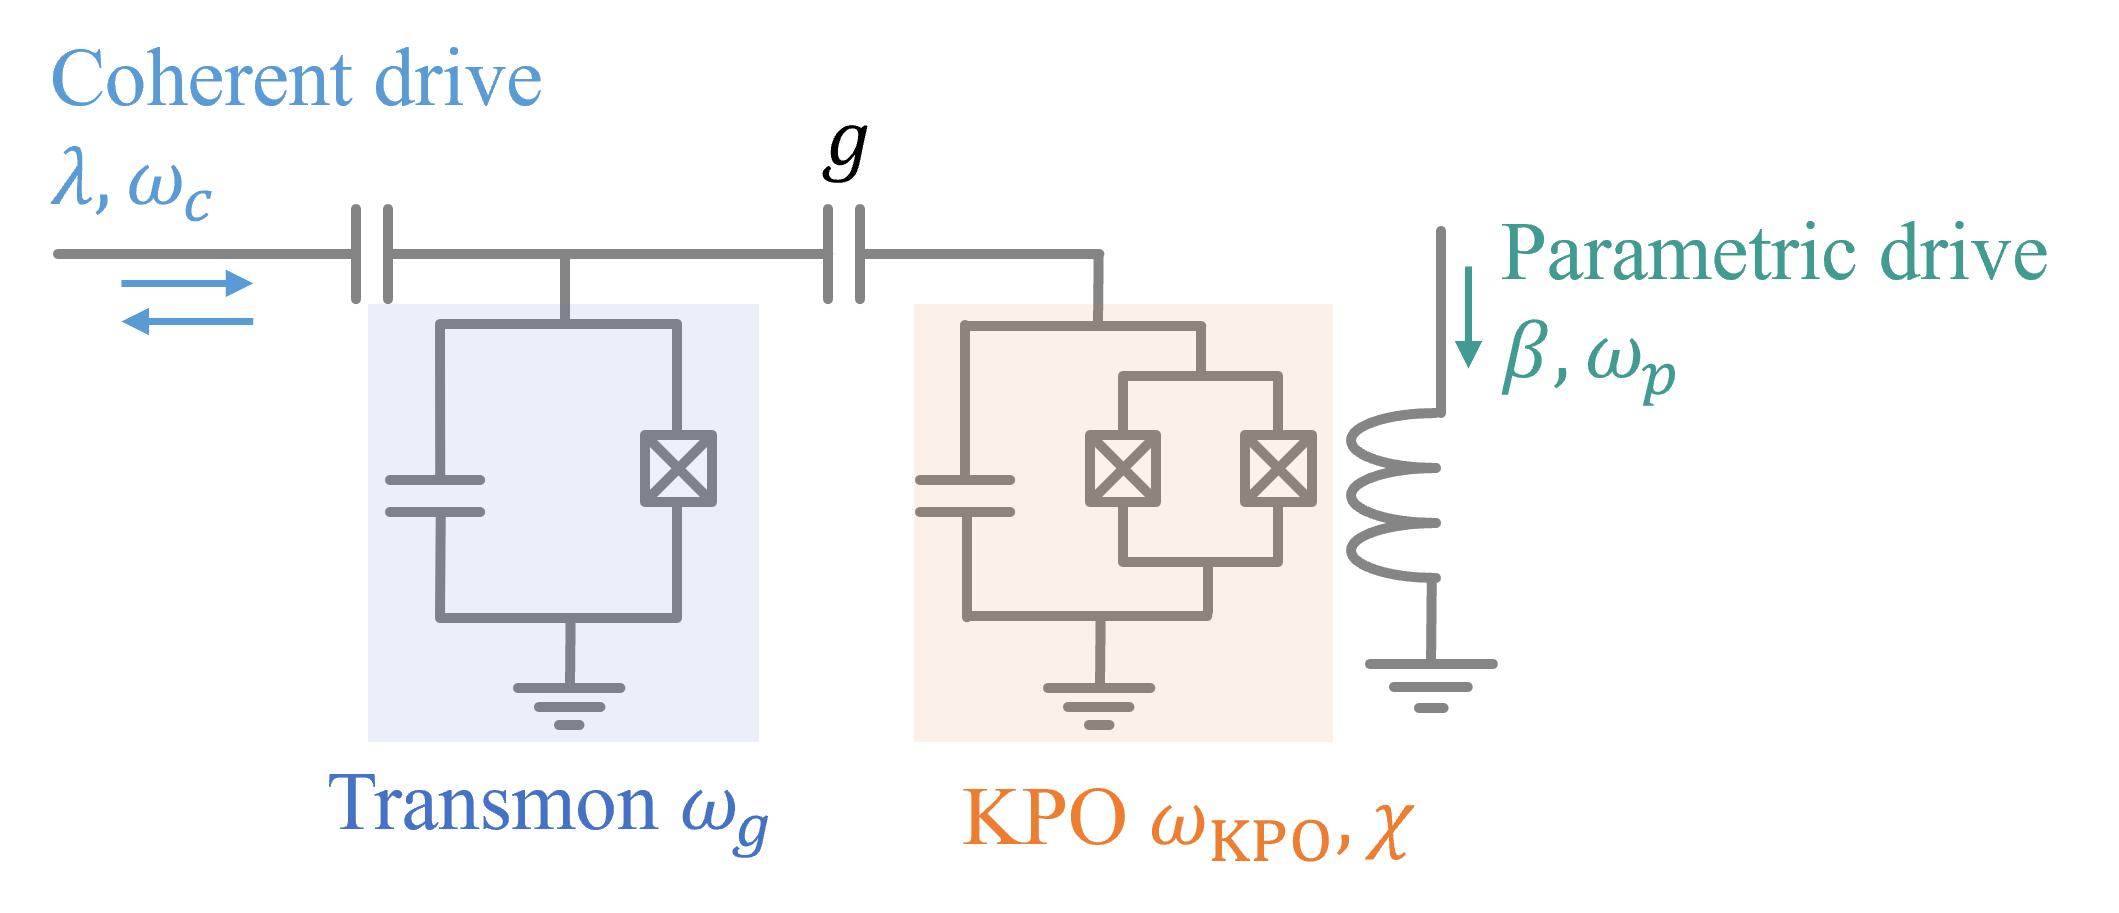
\includegraphics[width=9.1cm]{fig/fig1mod.png} \\
\caption{Schematic of a KPO coupled with a transmon qubit.
The transmon qubit is coupled to a transmission line. By driving the qubit through the transmission line and measuring the reflected fields, we can readout the information of the transmon qubit.
%To measure the population of the transmon qubit, we couple a resonator with the transmon qubit.
}
\label{fig:schematic1}
\end{figure}

In this paper, we propose a method to estimate the number of photons of the KPO from spectroscopic measurement. We consider a system, where the KPO is coupled with an ancillary qubit such as a superconducting transmon qubit or another KPO (without parametric drive), as shown in Fig.~\ref{fig:schematic1}. 

\subsection{ポピュレーションの測定および読み出し方法について}
平均光子数を推定するためには,スペクトルを実験的に測定する必要がある.そのためには,量子ビットの$\hat{\sigma}_z$の値を測定する必要がある.だから,量子ビットの状態読み出しのための共振器が必要となる.しかし,我々の手法では,補助量子ビットとトランスミッションラインは結合しており,トランスミッションラインを通して,量子ビットを駆動し,反射場を測定することによって,量子ビットの情報(スペクトル)を読み出すことが可能である~\cite{astafiev2010resonance,masuda2021theoretical}.そのため,読み出し用の共振器は不要である.そのため,我々はスペクトルを測定するために,基本的に反射測定を利用し,分散読み出しはオプションとして使うことが可能である.分散読み出しを使用する場合は,トランズモン量子ビットのポピュレーションを測定するために,分散読み出し用 (dispersive readout) の量子ビットと共振器を結合させることも可能である~\cite{mallet2009single,walter2017rapid,vijay2011observation}.
We show that spectroscopic measurements on the ancillary qubit provide an estimate of the number of photons of the KPO. We evaluate the performance of our method with numerical simulations by solving a master equation and show that the proposed method is more accurate than the conventional method.
It is worth mentioning that, in our previous study, by numerical methods, we investigate a case only when the driving strength is weak and the rotating wave approximation is valid\cite{2022ssdmkm}.
On the other hand, in this paper, by using both numerical and analytical methods, we analyze the case with strong driving
where the rotating wave approximation is violated. 
Moreover, in this paper, we study how the performance of our scheme changes with the detuning of the KPO.
These results in this paper provide a deep understanding of our scheme to estimate the number of photons.

The paper is organized as follows. In Sec. II, we introduce a model of a KPO coupled with an ancillary qubit. In Sec. III, we describe our method to estimate the number of the photons of the KPO by spectroscopic measurements.
In Sec. IV, we evaluate the performance of our method by using numerical simulations.
In Sec. V, we conclude our discussion.
Throughout this paper, we set $\hbar=1$.






\section{MODEL HAMILTONIAN}\label{Model}
In this section, we introduce a model of a KPO coupled 
with an ancillary qubit.
The Hamiltonian is given by
\begin{align}
    \hat{H}&=\omega_{\rm{KPO}}\ \hat{a}^\dagger\hat{a} - \frac{\chi}{12} (\hat{a}+\hat{a}^\dagger)^4 + 2\beta (\hat{a} + \hat{a}^{\dagger})^2\cos{\omega_{\rm{p}} t}\nn[10pt]
    &+\frac{\omega_{\rm{g}}}{2}\hat{\sigma}_z
    +g(\hat{a}+\hat{a}^\dagger)\hat{\sigma}_x
    +\lambda \hat{\sigma}_x \cos{\omega_c t},
\end{align}
where $\hat{a}^\dagger$ ($\hat{a}$) is a creation
(annihilation) operator of the KPO, $\omega_{\rm{KPO}}$ is the frequency of the KPO, $\chi$ is the Kerr coefficient, $\beta$ is the amplitude of a parametric drive, $\omega_{\rm{p}}$ is the frequency of the
parametric drive, $\omega_{\rm{g}}$ is the frequency of the ancillary qubit, $g$ is the coupling 
strength between the
KPO and the ancillary qubit, 
and $\lambda$ $(\omega_c)$ is the amplitude (frequency) of the driving field for the qubit, respectively. Here, $\hat{\sigma}_x$ and $\hat{\sigma}_z$ denote the Pauli operators.
Moving into a rotating frame at the frequency of $\omega_{\rm{p}}/2$ and adapting the rotating wave approximation, the Hamiltonian is written as
\begin{align}\label{total hamiltonian}
  \hat{H}&=\hat{H}_{\rm{KPO}}+\hat{H}_{\rm{G}}+\hat{H}_{\rm{I}}+\hat{H}_{\rm{D}},\\[10pt]
    \hat{H}_{\rm{KPO}}&=\Delta \hat{a}^\dagger\hat{a} - \frac{\chi}{2} \hat{a}^\dagger\hat{a}^\dagger\hat{a}\hat{a} + \beta (\hat{a}^2 + \hat{a}^{\dagger 2})\\[10pt]
    \hat{H}_{\rm{G}}&=\frac{\omega_{\rm{g}}-\omega_{\rm{p}}/2}{2}\hat{\sigma}_z\\[10pt]
    \hat{H}_{\rm{I}}&=g(\hat{a}\hat{\sigma}_{+}+\hat{a}^\dagger\hat{\sigma}_{-})\\[10pt]
    \hat{H}_{\rm{D}}&=\lambda_{\rm{p}}\left(\hat{\sigma}_+ e^{-i(\omega_c-\omega_{\rm{p}}/2)t}+\hat{\sigma}_- e^{i(\omega_c-\omega_{\rm{p}}/2)t}\right),
\end{align}
where $\Delta = \omega_{\rm{KPO}} -\chi - \omega_{\rm{p}}/2$ denotes the detuning of the KPO,  $\lambda_{\rm{p}}={\lambda}/{2}$ denotes the Rabi frequency of the ancillary qubit, and $\hat{\sigma}_{\pm}$ denotes the ladder operator.
Throughout our paper, we set $\Delta <0$.
%, which is typical for the experiment~\cite{yamaji2022spectroscopic}.
The ground and the first excited states of $\hat{H}_{\rm{G}}$ are $|{\rm{g}}\rangle $ and $|{\rm{e}}\rangle $, respectively. With $\beta =0$, %the lowest for eigenstates  are (in ascending order) 
the Fock states
$\ket{n}$ (for $n=0,1,2, 3$) become eigenstates of the
$H_{\rm{KPO}}$. For $\beta \gg |\chi|$, on the other hand, the corresponding eigenstates are approximately given by $(|\alpha \rangle+ |-\alpha \rangle )/\sqrt{2}$, $(|\alpha \rangle- |-\alpha \rangle )/\sqrt{2}$, $({\it{D}}_{\alpha}+{\it{D}}_{-\alpha})|1\rangle /\sqrt{2}$, and 
$({\it{D}}_{\alpha}-{\it{D}}_{-\alpha})|1\rangle /\sqrt{2}$, where ${\it{D}}_{ \alpha}=\exp{(\alpha\hat{a}-\alpha^{\ast}\hat{a}^\dagger)}$
denotes a displacement operator~\cite{goto2016bifurcation}.



\subsection{分散読み出しによる平均光子数推定の困難さ}
トランズモン量子ビットが線形共振器(調和振動子)を結合してるとき,$H'_{\rm{I}}=g \hat{\sigma}_z \hat{a}^{\dagger} \hat{a}$で記述される分散的相互作用 (dispersive interaction) を実現することができる.
この場合,トランズモン量子ビットを用いることで,共振器の平均光子数を測定することができる~\cite{johnson2010quantum,PhysRevApplied.14.044022,PhysRevX.11.031045,PhysRevA.103.023705}. 
しかし,我々の知る限り,トランズモン量子ビットとパラメトリックドライブで駆動されるKPOとの間の分散的相互作用を実現する手法は存在しない.さらに,$H'_{\rm{I}}=g \hat{\sigma}_z \hat{a}^{\dagger} \hat{a}$ は$\hat{H}_{\rm{KPO}}$と非可換である.このような非可換な相互作用は測定対象系の情報を読み出すために適していないことが知られている \cite{endo2020projecting}.
原理的には,パラメトリックポンプと非線形性を素早くオフにすれば($\beta=\chi=0$),KPOは線形共振器と同等になり,KPOの周波数をトランスモン量子ビットの周波数から離調させることで分散的相互作用を実現することが可能である. 
しかし,この場合,パルス操作を含む高速な測定が必要となり,連続波の測定だけで済む我々の提案する手法よりもはるかに困難である.


回転座標系でのHamiltonianの導出については,Appendix\ref{}を参照


\section{Methods}
In this section, we propose a method to estimate the number of photons of the KPO from a spectroscopic measurement of an ancillary qubit coupled with the KPO. As we explained,
for sufficiently large $\beta$, the ground state of the KPO is approximately described by a superposition of two coherent states, namely $|\alpha\rangle$ and $|-\alpha\rangle$ where $\pm \alpha$ is the amplitude of the coherent state. Without loss of generality, we can assume that $\alpha$ is a real number. Then, the Hamiltonian of the ancillary qubit is approximately written as

\begin{align}\label{qubit_Hamiltonian}
    \hat{H}_{\rm{qubit}}^{\rm{eff}}
    &=\frac{\omega_{\rm{g}}-\omega_{\rm{p}}/2}{2}\hat{\sigma}_z
    \pm 
    g\alpha\ \hat{\sigma}_x\nn[10pt]
    &+\lambda_{\rm{p}}\left(\hat{\sigma}_+ e^{-i\Delta _{\rm{q}}t}+\hat{\sigma}_- e^{i\Delta _{\rm{q}}t}\right),
\end{align}
where $\Delta _{\rm{q}}=\omega_c-\omega_{\rm{p}}/2$ denotes a detuning of the coherent drive
%the ancillary qubit 
\cite{goto2016bifurcation}.


It is known that we can observe a Mollow triplet via a spectroscopic measurement with this Hamiltonian, where resonant transition frequencies are 
$\Delta _{\rm{q}}=0$, $\pm 2g\alpha$~\cite{Mollow:1969zz,wu1994phase,wrigge2008efficient,ulhaq2012cascaded,xu2007coherent,laucht2017dressed}.
Since we can estimate the value of $g$ from a separate spectroscopic measurement by observing a vacuum Rabi splitting \cite{wallraff2004strong,chiorescu2004coherent}, 
we can obtain the value of $\alpha$ from the peak (dip) positions observed in the Mollow triplet.
It is worth mentioning that our method using the ancillary qubit
may affect the dynamics of the KPO due to the resonant condition between the KPO and the ancillary qubit. This means that 
we may be unable to use our method to estimate the number of photons in the middle of computation. 


\subsection{量子計算中の本手法の影響について}
ただし,補助量子ビットを用いる本手法は,KPOと補助量子ビットが共振するため,KPOのダイナミクスに影響を与える可能性がある.
つまり,量子計算の途中で我々の手法を用いて光子数を推定することができなくなる可能性がある.  
しかし,量子アニーリングやゲート型量子計算では,計算終了時の読み出し直前で本手法を適用することができる.
また,計算を開始する前に本手法を用いて平均光子数を知ることも可能である.
このような場合,計算中に,KPOと補助量子ビットの間のdetuningを設定し,補助量子ビットがKPOのダイナミクスに影響を与えないようにすることができる.ただし,実際に解いているKPOのdetuningは変えないように注意する(計算中はトランズモンの共振周波数をKPOの共振周波数から離しておく).
したがって,本手法は,量子アニーリングやゲート型量子計算において特に有効であることがわかる.

QA前に本手法を用いて,KPOからの出力の振幅$|\alpha|^2$に対して光子数を求めておき,較正 (calibration) しておくことで,KPOからの出力の振幅を読むだけで光子数がわかる.


With a conventional method \cite{puri2017engineering}, an analytical formula under semi-classical approximations such as $\alpha_{\mathrm{ana}}=\sqrt{(2\beta+\Delta)/\chi}$ is used to estimate the number of photons of the KPO when $\beta$ is much larger than the decay rate $\gamma_1$.
% \YMdel{Strictly speaking, a decay rate $\gamma_1$ also affects the number of photons. However, since we use parameters $\beta$ which is much larger than the decay rate, we can ignore the effect of $\gamma_1$ for the estimation of the number of photons} %\cite{puri2017engineering}.
% \footnote{Strictly speaking, a decay rate $\gamma_1$ also affects the number of photons. However, since we use parameters $\beta$ which is much larger than the decay rate, we can ignore the effect of $\gamma_1$ for the estimation of the number of photons \cite{puri2017engineering}}. 
Importantly,
previous research shows that 
the
value 
of $\alpha_{\mathrm{ana}}=\sqrt{(2\beta+\Delta)/\chi}$
can provide a wrong estimate~\cite{kanao2021high} due to the violation of the approximation.
Therefore, it is crucial to adopt more reliable method to estimate the number of photons especially when the conventional method provides an inaccurate estimation.


\subsection{本手法を適用するための結合強度$g$について}
SSDMで質問があった,この手法が適応できる結合強度gについては,重要な点であると思うので,ぜひご検討いただけると幸いです.
単純にgと損失レートκとの比というよりは,コヒーレント状態の振幅αとの積,α*g(ピーク間の距離)と,おそらくκから決まるMollow triplet のピークの線幅の大きさの比で説明できるのでは?と期待しているのですが,いかがでしょうか?
もし,g=5MHz以外の計算,例えばgがκと同じくらい小さい時などの結果もあればぜひ見てみたいです.
私は既存のデバイスで実験したので,gは5MHzで固定でしたが,
この手法を利用することを想定して,新たにデバイスを設計しようと思った場合には,どういうgにする必要があるのかという示唆があると非常に有益であると思います


\section{Numerical simulations}
In this section, we evaluate the performance of our method by comparing with the conventional method using numerical simulations of the GKSL (Gorini-Kossakowski-Sudarshan-Lindblad) master equation.
Here, we adopt the Hamiltonian in Eq.~\eqref{total hamiltonian}.
To take the effect of photon loss into account, we use the following GKSL master equation

\begin{align}\label{Eq.GKSL}
\frac{\partial\rho}{\partial t} &= -i\left[\hat{H}_{\rm{KPO}}+\hat{H}_{\rm{G}}+\hat{H}_{\rm{I}}+\hat{H}_{\rm{D}} 
,\ \rho\right] \nn[10pt]
&+\frac{\gamma_1}{2} \left (2\hat a \rho \hat a^\dagger - \left\{ \hat a^\dagger \hat a, \rho \right\}\right)
+ \frac{\gamma_2}{2} \left (2\hat{\sigma}_{-} \rho \hat{\sigma}_{+} - \left\{ \hat{\sigma}_{+} \hat{\sigma}_{-}, \rho \right\}\right),
\end{align}
where $\gamma_1$ denotes the one photon dissipation rate of the KPO, $\gamma_2$ denotes the spontaneous emission rate of the ancillary qubit, and
$\hat{\rho}$ denotes the density matrix describing the quantum state of the total system.
We solve the GKSL master equation Eq.~\eqref{Eq.GKSL} using QuTiP~\cite{johansson2012qutip}.
We choose the initial state as a
steady state of Eq.~\eqref{Eq.GKSL} with $\lambda _{\rm{p}}=0$.
Also, we set $\omega_g=\omega_{\rm{p}}/2$.

\begin{figure}%[h]
\centering
		%\includegraphics[width=9.1cm]{fig/sigmaz_td_Detu_-30_Keer_18_pump_42_dec_0.8_L_0.5.pdf} \\
\caption{
(a) The time-integrated spectra $I$ against $\Delta_{\rm{q}}/2\pi$ with $\lambda_{\rm{p}}/2\pi=0.5$  MHz. We set the parameters as $\Delta/2\pi=-30.0$  MHz, $\chi/2\pi=18.0$ MHz, $\beta/2\pi=42.0$ MHz, $g/2\pi=5.0$ MHz, $\gamma_1/2\pi=\gamma_2/2\pi=0.8$ MHz, and $\omega_g=\omega_{\rm{p}}/2$.
(b)The energy diagram of the states of a KPO coupled with a qubit.
In the left (right) side, we show the energy diagram with $\beta/2\pi=0$ MHz ($\beta\gg |\chi|$). Here,
$|\alpha \rangle $ and $\ket{n}$ (for $n=0,1,2$) denote a coherent state
 and Fock states, respectively, while
${\it{D}}_{ \alpha}=\exp{(\alpha\hat{a}-\alpha^{\ast}\hat{a}^\dagger)}$
denotes the discplacement operator. 
% Here,
% $\ket{\rm{vac}}$,  $|\alpha \rangle $, and $\ket{n}$ (for $n=1,2$) denote the vacumme state, coherent state, and Fock states, respectively, while 
% %${\it{D}}_{\pm \alpha}$
% ${\it{D}}_{ \alpha}=\exp{(\alpha\hat{a}-\alpha^{\ast}\hat{a}^\dagger)}$
% denotes the discplacement operator. 
%such as ${\it{D}}_{\pm \alpha} |\rm{vac}\rangle = |\pm \alpha \rangle $. 
Also, $|g\rangle $ ($|e\rangle $) and $|\pm \rangle =\frac{1}{\sqrt{2}}(|g\rangle \pm |e\rangle )$
denotes the ground (excited) state and the superposition states of the qubit.
}
\label{fig:spect1}
\end{figure}




In Fig.~\ref{fig:spect1} (a), we plot a time-integrated spectra $I=(1/t)\int_{0}^{t}\ d\tau\ (\braket{\hat{\sigma}_z}+1)/2$ as a function of $\Delta_{\rm{q}}$ with a step of $0.05$ MHz,
where $\braket{\hat{\sigma}_z}={\rm{Tr}}[\hat{\sigma}_z \rho ]$,
which is effectively the same as a spectroscopy to detect the change in the pupulation of the qubit.

%\YM{We can interprete the three relevant transitions between them as the Mollow triplet of the ancillary qubit where the coupling with the KPO plays a role of the driving field on the qubit.}
%In Fig.~\ref{fig:spect1} (a),
This spectra is upper (lower) bounded by $1$ ($0$).
The value of this spectra depends on the Rabi frequency and decay rate of the qubit.
The observed peak and dips are at $\Delta_{\rm{q}}^{(0)}/2\pi=1.35$ MHz, $\Delta_{\rm{q}}^{(1)}/2\pi= -16.80$ MHz and $\Delta_{\rm{q}}^{(2)}/2\pi = 17.10$ MHz, respectively.
% The observed peaks are at $\Delta_{\rm{q}}^{(0)}/2\pi=1.35$ MHz, $\Delta_{\rm{q}}^{(1)}/2\pi= -16.80$ MHz , and $\Delta_{\rm{q}}^{(2)}/2\pi = 17.10$ MHz.

Fig.~\ref{fig:spect1} (b) shows the energy diagram composed of the system of the KPO coupled with an ancillary qubit.
We calculate the energy eigenvalues of the Hamiltonian, and we confirm that the energy difference between the eigenvalues is almost the same as the peak frequency observed in our numerical simulation.
The dip at $\Delta_{\rm{q}}^{(1)}/2\pi= -16.80$ MHz ($\Delta_{\rm{q}}^{(2)}/2\pi = 17.10$ MHz) corresponds to the transition between the ground (first excited) state and the second (third) excited state, which we describe by a red vertical arrow in Fig.~\ref{fig:spect1} (b).
Here, with our parameters, the ground state, first excited state, second excited state, and third excited state 
 are approximately described as
$\ket{-}(\ket{\alpha}+\ket{-\alpha})$,
$\ket{-}(\ket{\alpha}-\ket{-\alpha})$,
$\ket{+}(\ket{\alpha}+\ket{-\alpha})$, and
$\ket{+}(\ket{\alpha}-\ket{-\alpha})$, respectively.
%$\ket{-}(\hat{D}_{\alpha}+\hat{D}_{-\alpha})\ket{2}$ to $\ket{-}(\hat{D}_{\alpha}-\hat{D}_{-\alpha})\ket{2}$,  
 %$\ket{-}(\ket{\alpha}-\ket{-\alpha})$
 On the other hand, the peak at $\Delta_{\rm{q}}^{(0)}/2\pi=1.35$ MHz corresponds to a transition between the fourth excited state and the fifth excited state, which we describe by a green vertical arrow in Fig.~\ref{fig:spect1} (b),
 where the fourth (fifth) excited state is approximately given as $\ket{-}(\hat{D}_{\alpha}+\hat{D}_{-\alpha})\ket{2}$ ($\ket{-}(\hat{D}_{\alpha}-\hat{D}_{-\alpha})\ket{2}$).
Actually, from the numerical simulation, the population of the fourth  (fifth) excited state at $t=0$ is $0.00590$ (0.0173) and becomes finally $0.00772$ (0.0155) at $t=3$ $\mu$s. This means that the coherent drive actually induces a transition between the fourth excited state and the fifth excited state.
By diagonalizing the Hamiltonian, we recognized that we have a transition between the second excited state and the third excited state
 with an energy difference of
 $2\pi \times 0.5$ MHz.
 However, we cannot resolve this peak in the numerical simulation possibly due to the large width of the peak at $\Delta_{\rm{q}}^{(0)}$.




% \KM{In Fig.~\ref{fig:pump_effect}, we describe a effect of an parametric drive occur the transition $\Delta E_{4,5}$.
% In Fig.~\ref{fig:pump_effect}, we plot a transition frequency $\Delta_{\rm{q}}^{(0)}$ against a amplitude of a parametric drive $\beta$.
% From Fig.~\ref{fig:pump_effect}, we find $\Delta_{\rm{q}}^{(0)}$ is equal to $\Delta E_{4,5}$ at $\beta/2\pi/ = 42.0$ MHz.}

Now, let us discuss the estimation of the number of photons.
We consider a steady state $\hat{\rho}_{\rm{ss}}$ of Eq.~\eqref{Eq.GKSL} with $\lambda_{\rm{p}}=0$ and $g=0$, and we define $\rm{Tr}[\rho_{\rm{ss}}\hat{a}^\dagger\hat{a}]=|\alpha|^2$.
Let us define a
 relative error of $|\alpha|^2$ estimated by using our method as $\epsilon_1\equiv||\alpha_{\rm{est}}|^2-|\alpha|^2|/|\alpha|^2$, where $|\alpha|^2$($|\alpha_{\rm{est}}|^2$) is the actual (estimated) value of the photon number of the KPO.
Also, when we use the analytical formula, the relative error of the estimated $|\alpha|^2$ is
defined as $\epsilon_2\equiv||\alpha_{\rm{ana}}|^2-|\alpha|^2|/|\alpha|^2$.

From Fig.~\ref{fig:spect1} (a), we observe two dips at
$\Delta ^{(1)}_{\rm{q}}$ and $\Delta ^{(2)}_{\rm{q}}$ and the frequency difference is $(\Delta ^{(2)}_{\rm{q}}-\Delta ^{(1)}_{\rm{q}})/2\pi=33.90$ MHz. We can estimate the number of photons from this, as we explained before.
Since we set $g/2\pi=5$ MHz, 
we obtain an estimated value of 
$|\alpha _{\rm{est}}|^2= 2.87$,
where we solve an equation of $4g\alpha _{\rm{est}}/2\pi=(\Delta ^{(2)}_{\rm{q}}-\Delta ^{(1)}_{\rm{q}})/2\pi=33.90$ MHz.
The relative error is calculated as
$\epsilon_1=0.0280$.
On the other hand, when we use the analytical formula, we obtain $\epsilon_2=0.0672$.
This result indicates that our method provides a more accurate estimate of $\alpha$ than the conventional method. 

% \KM{Here, we observe the peak at $1.3$ MHz which shifted from $0$ MHz.
% We consider this shift is caused by a effect of the pump.
% We plot plot }

\begin{figure}%[h]
\centering
		%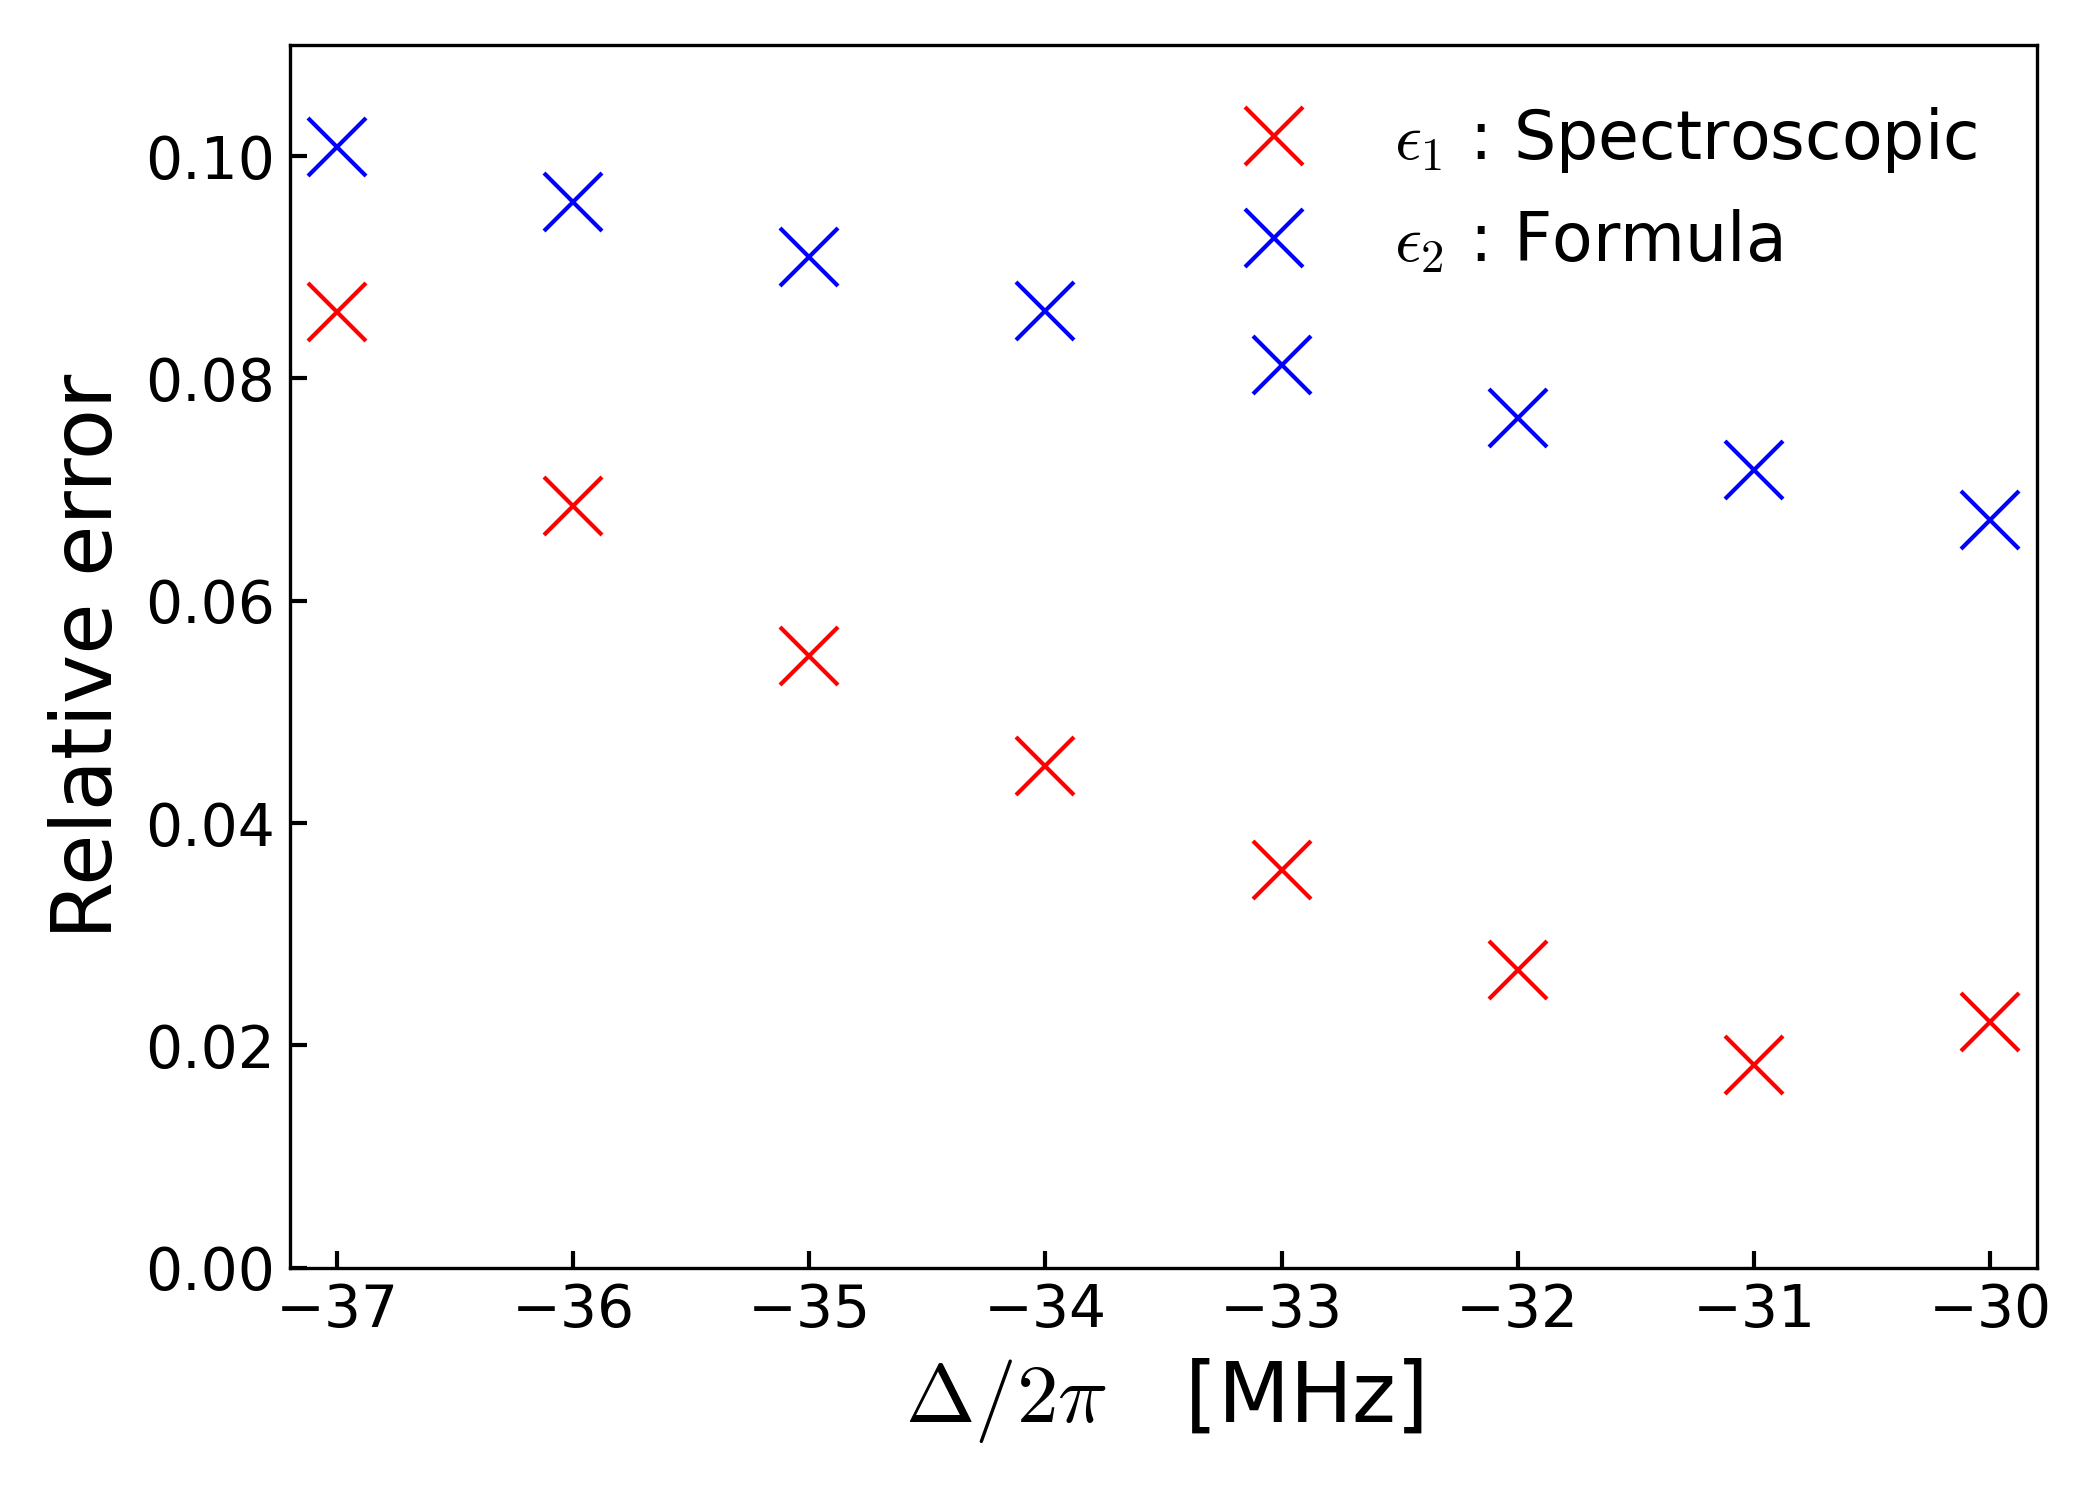
\includegraphics[width=9.1cm]{fig/alpha_estimete_meannum.png} \\
\caption{
Plot of the relative error $||\alpha_{\rm{est}}|^2-|\alpha|^2|/|\alpha|^2$ 
against the detuning of the KPO
 where $|\alpha|^2$ ($|\alpha_{\rm{est}}|^2$) is the true (estimated) value of the photon number.
 We set the parameters as $\chi/2\pi=18.0$ MHz, $\beta/2\pi=42.0$ MHz, $g/2\pi=5.0$ MHz, $\lambda_{\rm{p}}/2\pi=0.5$ MHz, $\gamma_1/2\pi=\gamma_2/2\pi=0.8$ MHz, and $\omega_g=\omega_{\rm{p}}/2$.
}
\label{fig:spec_error1}
\end{figure}

 

\begin{figure}%[h]
\centering
		%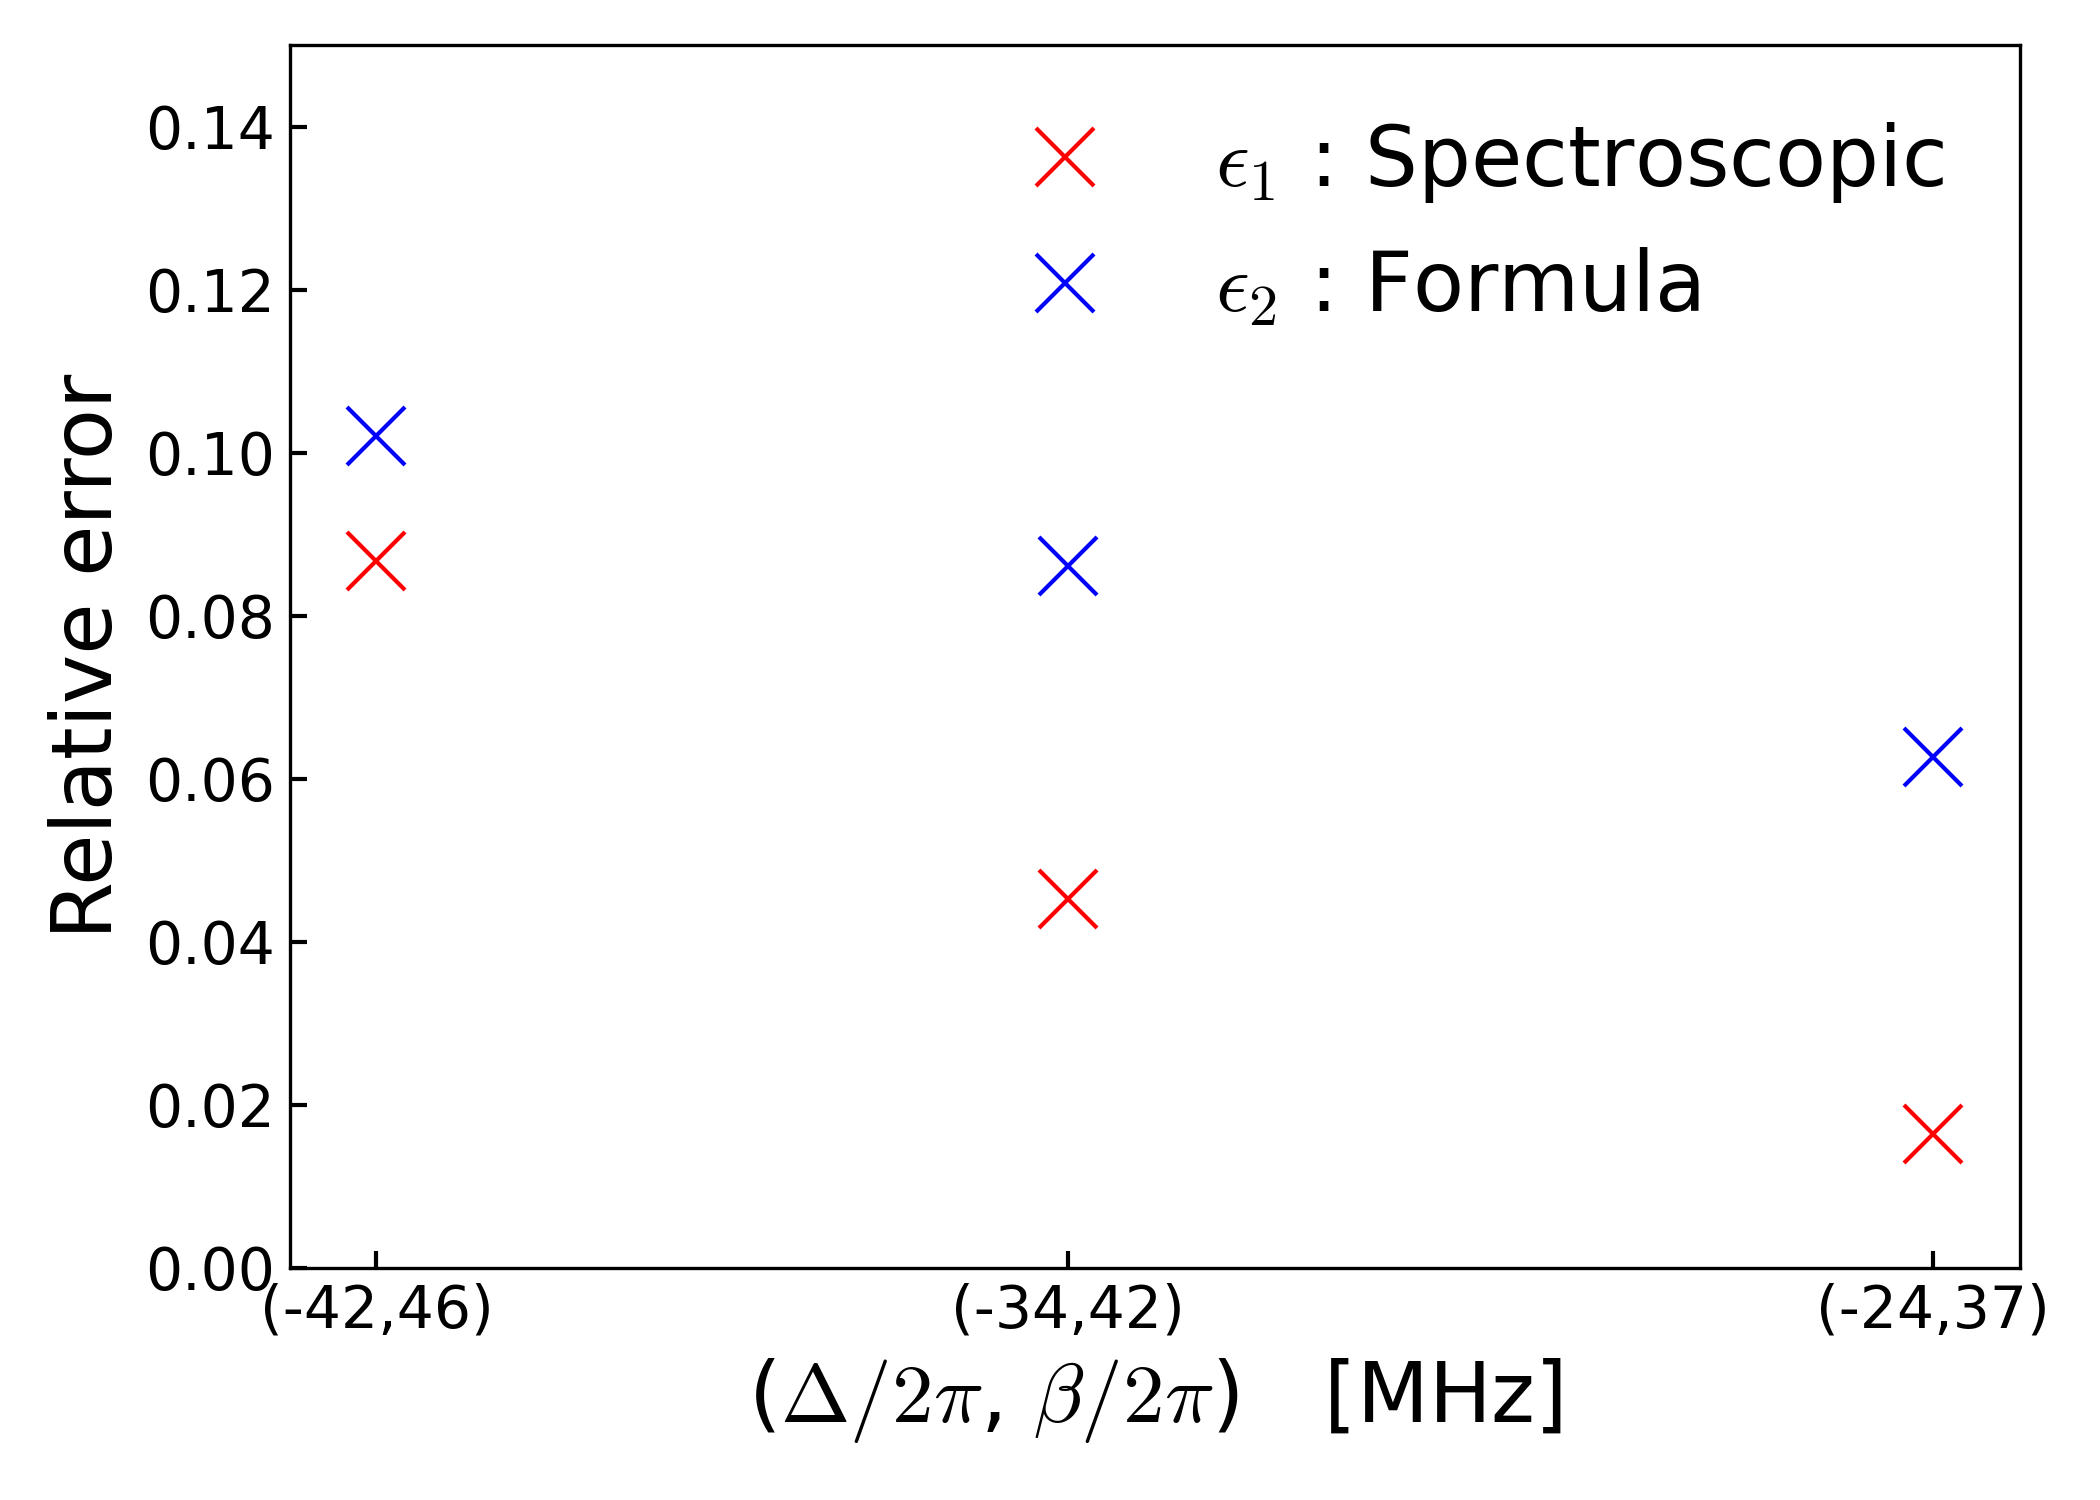
\includegraphics[width=9.1cm]{fig/alpha_estimete_meannumber2.png} \\
\caption{
Plot of 
the relative error $||\alpha_{\rm{est}}|^2-|\alpha|^2|/|\alpha|^2$ 
against the detuning of the KPO
 where $|\alpha|^2$ ($|\alpha_{\rm{est}}|^2$) is the true (estimated) value of the photon number.
We set $\beta$ to satisfy a condition of $(2\beta + \Delta)/2\pi = 50$ MHz.
Also, we set the parameters as $\chi/2\pi=18.0$ MHz, $g/2\pi=5.0$ MHz, $\lambda_{\rm{p}}/2\pi=0.5$ MHz, $\gamma_1/2\pi=\gamma_2/2\pi=0.8$ MHz, and $\omega_g=\omega_{\rm{p}}/2$.
}
\label{fig:spec_error2}
\end{figure}

\begin{figure}%[h]
\centering
		%\includegraphics[width=9.1cm]{fig/sigmaz_td_Detu_-34_Keer_18_pump_42_dec_0.8_L_2.pdf} \\
\caption{
(a) The time-integrated spectra $I$ against the detuning $\Delta_{\rm{q}}/2\pi$ with the Rabi frequency $\lambda_{\rm{p}}/2\pi=2$  MHz.
We use the same parameters as those in Fig.~\ref{fig:spect1} (a) except the Rabi frequency. 
We observe not only the main two dips but also small dips
at $\Delta _{\rm{q}}^{(3)}/2\pi=-8.40$ MHz and $\Delta _{\rm{q}}^{(4)}/2\pi=-8.65$ MHz. }

\label{fig:spec2}
\end{figure}

Also, to further quantify the performance of our method,
we calculate the relative error of our methods with other parameters, and compare the error with that of the conventional method.
When the detuning is too large for the KPO to bifurcate, the ground state of the KPO is not the superposition of the coherent states anymore. Thus, when we plot Figs.~\ref{fig:spec_error1} and \ref{fig:spec_error2}, we choose a range of detuning for the KPO to bifurcate in these numerical simulations.

% \footnote{
% When the detuning is too large for the KPO to bifurcate, the ground state of the KPO is not the superposition of the coherent states anymore. Thus, when we plot Figs.~\ref{fig:spec_error1} and \ref{fig:spec_error2}, we choose a range of detuning for the KPO to bifurcate in these numerical simulations.}.
In Fig.~\ref{fig:spec_error1}, we plot the relative error against the detuning of the KPO $\Delta$.
In Fig.~\ref{fig:spec_error2}, we plot the relative error against 
$\Delta$ by setting $\beta$ to satisfy a condition of $(2\beta + \Delta)/2\pi = 50$ MHz.
The reason why we choose this condition is that the estimated photon number $|\alpha_{\rm{ana}}|^2$ from the analytical formula is fixed in these numerical simulations.
From Figs.~\ref{fig:spec_error1} and~\ref{fig:spec_error2}, our method provides a more accurate estimate of $|\alpha|^2$ than the conventional method when there is a detuning $\Delta$. 
%\YM{In Fig.~\ref{fig:spec_error1}, we find that there is an optimal detuning to minimize the relative error
%for our method.
%This shows a non-monotonic dependence of the relative error on the detuning.
%}
Fig.~\ref{fig:spec_error1} shows a non-monotonic dependence of the relative error on the detuning. Thus, we find that there is an optimal detuning to minimize the relative error
for our method.
It is worth mentioning that, in the original proposal of QA with KPO \cite{goto2016bifurcation}, KPO has a finite detuning during QA. Therefore, our scheme is useful for such circumstances.


Furthermore, we investigate how a stronger Rabi frequency affects spectroscopic measurements.
We perform numerical simulations with a Rabi frequency
of
$\lambda /2\pi = 2$ MHz.
It is worth mentioning that
we observe not only the prominent two dips but also small dips
at $\Delta _{\rm{q}}^{(3)}/2\pi=-8.40$ MHz and $\Delta _{\rm{q}}^{(4)}/2\pi=8.65$ MHz, in Fig.~\ref{fig:spec2}.
We expect that these additional dips come from the violation of the rotating wave approximation, which  will be discussed in Appendix~\ref{purtabation}.

\subsection{photon lossによる実用上の問題について}
レフェリーによる有益なコメントに感謝する.確かに,我々の数値シミュレーションでは,光子の損失により,2つのコヒーレントな状態のインコヒーレントな混合が発生する.同様に,量子アニーリングにおける問題のハミルトニアンの基底状態が縮退している場合,光子の損失により基底状態のインコヒーレントな混合が発生します.しかし,実際の量子アニーリングでは,以下の理由により,実用上の問題は生じないはずです.量子アニーリングの主な対象である組み合わせ最適化問題では,縮退した基底状態のいずれかを得ることができれば計算は成功したとみなされる.そのため,量子アニーリング後に縮退した基底状態の古典的混合状態を得る場合,その状態を読み出すだけで,いずれかの基底状態を得ることができる.この点については,修正原稿で説明しています.

Let us remark that, although the ground state of the KPO is a superposition of two coherent states, we have a classical mixture of two coherent states in our numerical simulations
due to the photon loss.
Similary, if we perform quantum annealing with a problem Hamiltonian whose ground states are degenerate, we will obtain not the superposition of the ground states but the classical mixture between them.
Fortunately, this does not affect the performance of QA for the following reason.
When we solve combinational optimization problems with QA, the purpose is not to obtain all degenerate ground states 
but to obtain one of the ground state. So, even if the state after QA is a classical mixture of the degenerate ground states, single shot measurements of KPOs project the states into one of the ground states, and we obtain the answer. 


% \begin{figure}[h]
% \centering
% 		%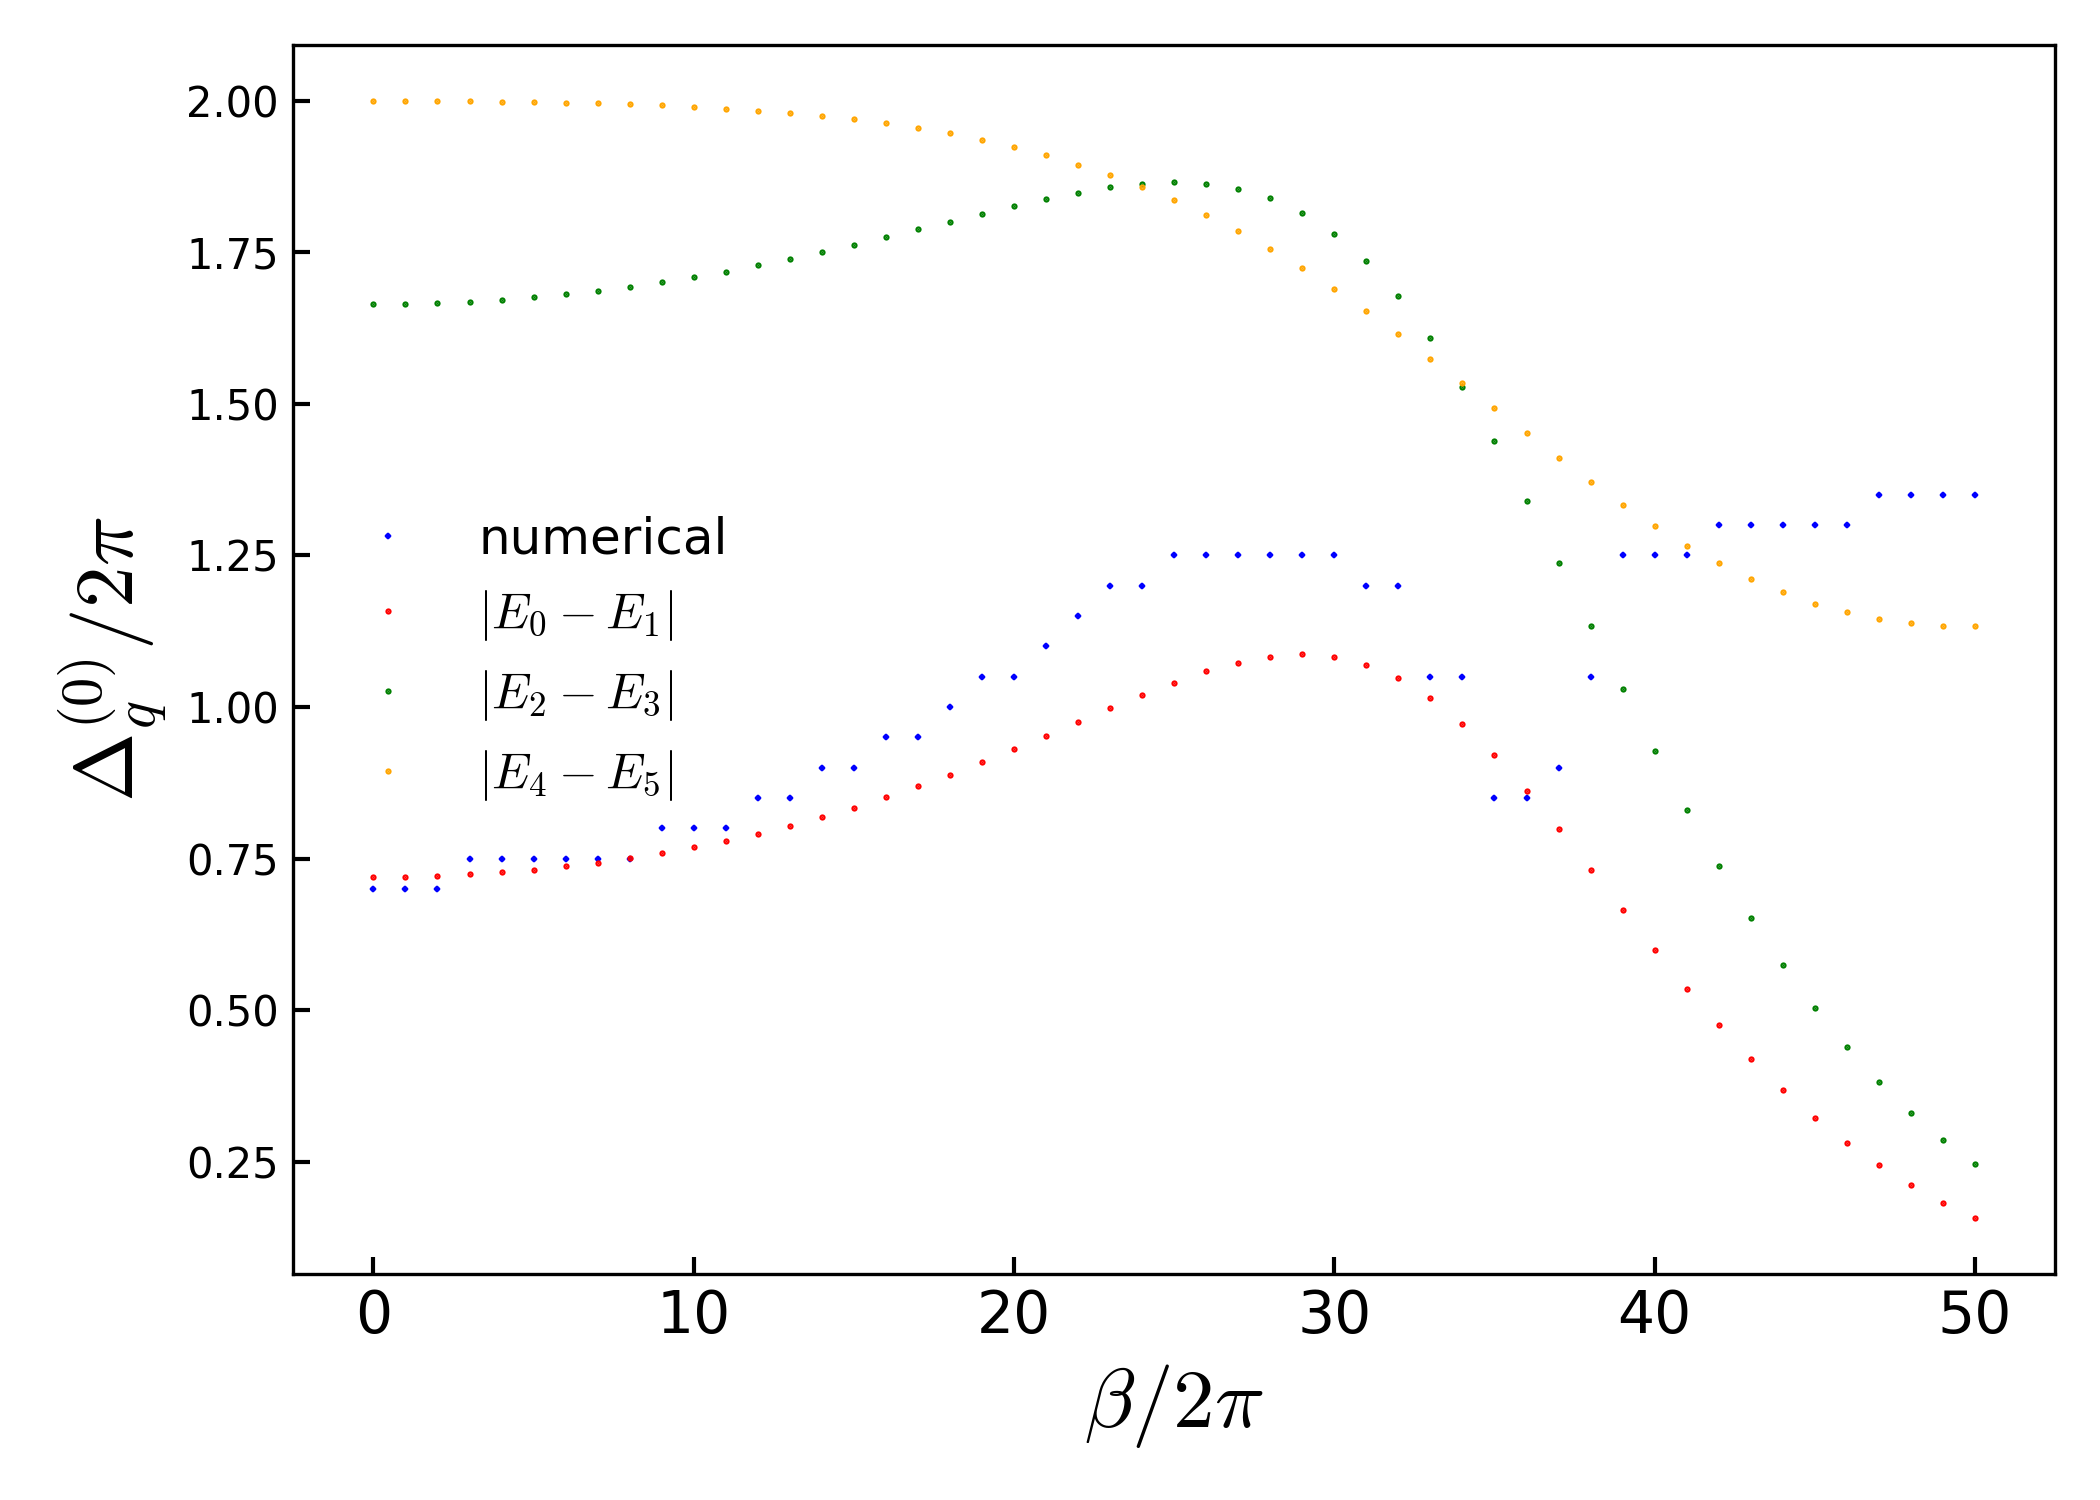
\includegraphics[width=9.1cm]{fig/spect_sigmaz_td1D_Detu_-34_Keer_18_dec_0.8_L_0.5.png} \\
% \caption{
% \KM{(a) The time-integrated spectra $I$ against $(\omega_{\rm{c}}-\omega_{\rm{p}}/2)/2\pi$ with $\lambda/2\pi = 0.5$ MHz.
% (b) Color map of the expectation values of $\hat{\sigma}_z$ againt $(\omega_{\rm{c}}-\omega_{\rm{p}}/2)/2\pi$ (x axis) for a given time (y axis) with $\lambda/2\pi = 0.5$ MHz.
% We set the parameters as $\Delta/2\pi = 100$ MHz, $\chi/2\pi = 18$ MHz, $\beta/2\pi = 20.0$ MHz, $g/2\pi = 5$ MHz.
% }The time-integrated spectra $I$ against $\Delta_{\rm{q}}/2\pi$ with $\lambda_{\rm{p}}/2\pi=0.5$  MHz. We set the parameters as $\Delta/2\pi-34.0$  MHz, $\chi/2\pi=18.0$ MHz, $\beta/2\pi=42.0$ MHz, $g/2\pi=5.0$ MHz, and $\omega_g=\omega_{\rm{p}}/2$.}
% \label{fig:pump_effect}
% \end{figure}

\section{Conclusion}
In conclusion, we propose an experimentally feasible method to estimate the number of photons of the KPO. We couple an ancillary qubit with the KPO, and spectroscopic measurements of the qubit let us know the number of photons of the KPO. Our results are essential to realize QA with KPOs for solving combinational optimization problems.




\section{議論}
松崎様

 

山本です.

少し私からもコメントさせてください.

 

今問題となっているコメントは,査読者が,

・光子数を決めるためには,Fig. 2aに相当するものを実験で測定する必要がある.

・そのためには量子ビットのσzを測定する必要がある,

・だから量子ビットの状態読出しのための共振器が必要だろう

と考えたからだと思います.

 

ですが,我々としては,Fig. 2aに相当するものは量子ビットの反射測定で測ることを意図していたので,

読出しの共振器は不要で,Fig. 1にも描いていなかったということだと思います.

 

実際のところ,読出し共振器を設けて量子ビットの状態を測定することは勿論可能ですが,

実験的には量子ビットを直接反射測定するより大分複雑になるので,

本論文で主張している簡便な方法という点が弱くなってしまいます.

 

ですので,(山口さんのメールの前に)山口さんと相談した時は,

反射測定を基本とするべき(分散読出しはオプションとしてはあり)なので,

Fig. 1には読出し共振器は描かない方が良い,と考えました.

 

そのためには,Fig. 2aに相当するものを反射測定で測れるということを,

説明できるかどうかがポイントだと思います.

例えば,材料として,

増田さんのNew J. Phys. 23 (2021) 093023の論文

(対象はKPOですが,Eq. 30, 31に反射係数と密度行列の対角成分の関係式がある)や

実験ではAstafiev et al., Science 327, 841 (2010)

(Fig. 1c 導波路に磁束量子ビットが直接結合した系の透過率が,量子ビットの励起により変化する)

が使えるのではないかと思います.

 

よろしくお願いします.

 




松崎です.
海外出張中で対応が遅れてすみません.

いろいろと考えたのですが,dispersive measument のセットアップを書きつつ,本文中(およびcaption)で,トランズモン量子ビットへプローブ光をいれて分光測定することも可能であると書くのが良い気がします.

ちなみに来週は産総研の火曜日以降にはいらっしゃいますでしょうか?
少し議論できれば幸いです.

 

お世話になっております.山口です.

お返事が遅くなり申し訳ありません.

 

Referee1からのコメントに関して,図を作成すること自体は問題ないのですが,

1点確認させてください.

今回の測定では,transmon(またはtransmon動作しているKPO)を想定していており,

それを”分光測定”するという簡便な方法で光子数がわかる,ということがミソであったと思います.

この分光測定はdispersive readout を行うのではなく,直接transmonにプローブを入れて

その反射測定をするものだと思っていたので,readout resonatorは必要ない,

と思っていたのですが,いかがでしょうか?

 

これに類する実験として,以前に私が2KPO系で測定した際には,

ポンプしていない側のKPO(今回のtransmon)を直接分光していました.

 

Dispersive readoutで同様の測定をすることも不可能ではないとは思うのですが,

簡便性という観点からも,直接の分光をする,という主張のほうがシンプルに思います.

 

以上,ご検討いただけますと幸いです.

どうぞよろしくお願いいたします.





山本様へ

いつもお世話になっております松崎です.
「
Fig. 1で

Coherent driveと書かれたポートが

それだと思います.

」

なるほど.了解いたしました.
丁寧な返信をありがとうございます.大変勉強になりました.

松崎 雄一郎


差出人: YAMAMOTO TSUYOSHI(山本 剛)
送信: 2022 年 12 月 12 日 (月曜日) 8:57
宛先: 松崎雄一郎
Cc: 松本佳大; 山口愛子
件名: RE: Our initial decision on your article: JJAP-S1102957

松崎様

 

ちなみに,我々のスキームで反射測定を行う場合,トランズモン量子ビットにtransmission lineを結合させる必要があると思いますが,その理解であっておりますでしょうか?
 

Fig. 1で

Coherent driveと書かれたポートが

それだと思います.

 

もしそうだとすると,トランズモン量子ビットにtransmission lineが結合した図が必要かと思いました.
 

上記の通り,現在の図はすでにそうなっていると私は理解しています.

 

よろしくお願いします.

山本剛

From: 松崎雄一郎 <matsuzaki.yuichiro@aist.go.jp>
Sent: Monday, December 12, 2022 8:46 AM
To: YAMAMOTO TSUYOSHI(山本 剛) <tsuyoshi.yamamoto@nec.com>
Cc: 松本佳大 <matsumoto-kei@aist.go.jp>; 山口愛子 <aiko-uchiyama@aist.go.jp>
Subject: Re: Our initial decision on your article: JJAP-S1102957

 

山本様へ

 

松崎です.返信ありがとうございます.

なるほど.反射測定でも,JPAをつかうことでsingle shot readoutが可能なのですね.

よくわかりました.

 

ちなみに,我々のスキームで反射測定を行う場合,トランズモン量子ビットにtransmission lineを結合させる必要があると思いますが,その理解であっておりますでしょうか?

 

もしそうだとすると,トランズモン量子ビットにtransmission lineが結合した図が必要かと思いました.

 

松崎雄一郎

 

 

差出人: YAMAMOTO TSUYOSHI(山本 剛)
送信: 2022 年 12 月 11 日 (日曜日) 22:31
宛先: 松崎雄一郎
Cc: 松本佳大; 山口愛子
件名: RE: Our initial decision on your article: JJAP-S1102957

 

松崎様

 

ご返信ありがとうございました.

 

反射測定もsingle-shot readoutは可能です.

 

1~10程度の平均光子数のプローブ信号強度かつ~20 dBのゲインのJPAを用いた場合,

dispersive readout,反射測定共に~100 nsが標準的な読出し時間と思います.

 

よろしくお願いします.

山本剛

From: 松崎雄一郎 <matsuzaki.yuichiro@aist.go.jp>
Sent: Sunday, December 11, 2022 8:06 PM
To: YAMAMOTO TSUYOSHI(山本 剛) <tsuyoshi.yamamoto@nec.com>
Cc: 松本佳大 <matsumoto-kei@aist.go.jp>; 山口愛子 <aiko-uchiyama@aist.go.jp>
Subject: Re: Our initial decision on your article: JJAP-S1102957

 

山本様へ

返信ありがとうございます.

 

では両方について言及して,共振器は書かない方針で行きたいと思います.

 

「

ちなみに分散読出しのほうが,反射測定よりも早く読めるとお考えの理由は何でしょうか?

スピードを決めているのは,読出し共振器や量子ビットと伝送線路の結合強度と,

読出しのプローブ信号強度と思いますが,どちらも大きな差はないように思っています.

」

 

ここは私の勘違いがあるのかもしれません.

お手数をおかけしますが,以下の私の理解が正しいか,お教え頂ければ幸いです.

 

共振器を用いてdispersive readoutができる場合は,single shot readoutが可能です.

そのため,数十ns程度で,qubitのアップかダウンかを判定できます.

 

反射測定の場合は,single shot readoutができないので繰り返し計測する必要があります.

数十nsで読む出すことは,かなり難しいと思います.

 

いかがでしょうか?

私が何か勘違いしているかもしれません.その場合は申し訳ございません.

 

松崎 雄一郎

 

 

差出人: YAMAMOTO TSUYOSHI(山本 剛)
送信: 2022 年 12 月 11 日 (日曜日) 10:41
宛先: 松崎雄一郎
Cc: 松本佳大; 山口愛子
件名: RE: Our initial decision on your article: JJAP-S1102957

 

松崎様

 

ご返信ありがとうございました.

 

両方について言及するのは良いと思います.

(私はやはり図に共振器は描かなくてよいと思います)

 

ちなみに分散読出しのほうが,反射測定よりも早く読めるとお考えの理由は何でしょうか?

スピードを決めているのは,読出し共振器や量子ビットと伝送線路の結合強度と,

読出しのプローブ信号強度と思いますが,どちらも大きな差はないように思っています.

 

よろしくお願いします.

山本剛

From: 松崎雄一郎 <matsuzaki.yuichiro@aist.go.jp>
Sent: Sunday, December 11, 2022 9:13 AM
To: YAMAMOTO TSUYOSHI(山本 剛) <tsuyoshi.yamamoto@nec.com>; 山口愛子 <aiko-uchiyama@aist.go.jp>
Cc: 松本佳大 <matsumoto-kei@aist.go.jp>
Subject: Re: Our initial decision on your article: JJAP-S1102957

 

山本様

 

いつもお世話になっております松崎です.

コメントありがとうございます.

 

「

ですので,(山口さんのメールの前に)山口さんと相談した時は,

反射測定を基本とするべき(分散読出しはオプションとしてはあり)なので,

Fig. 1には読出し共振器は描かない方が良い,と考えました.

」

 

たしかにその方針でも良いかもしれません.

 

ただ私として懸念していることを以下にあげます.

 

KPOで複雑な問題をQAで解いたときに,QAを終えた直後と,QAを終えてから(発振を続けていても)時間がたってからでは,KPOの光子数が変わる可能性があるという点です.

もちろん,T1の影響で|α>が|-α>になるだけであれば,平均光子数自体は変化しない気もします.

ただ,KPOの振る舞いは複雑なので,光子数が変わる可能性も否定はできないと思います.

 

 

反射測定で我々のプロトコルを実行する場合,KPOの光子数を読みだすのに時間がかかってしまうと思います.

dispersive測定で実行すれば,KPOの光子数を高速で読めると思います.

 

そのため,QAで終えた直後に,dispersive測定で高速にKPOの光子数を読み取れば,上のようなKPOの光子数が変わるという問題が起きないと思います.

 

ただ,この点はあくまでも懸念点程度で,実際に本当に問題になるかは自信がありません.

 

そのため両方の場合を書くのが無難かと考えております.

 

両方というのは

・高速でKPOの光子数を知りたい場合→dispersive測定

・時間をかけても良い場合→プローブによる反射測定

を説明するということです.(上の懸念点は,ちょっと自信がないので,具体的には書かないつもりです.あくまでも状況に応じて使い分けられるよね,と書く程度です)

 

その場合に,図に読み出しのためのresonatorを書くかどうかは悩ましいですが,書かないのもありかと思います.(その場合でも本文中にはdispersive測定の場合も書く予定です)

 


いかがでしょうか?

%\section{5,6, September, 2022}
SSDMに向けてスライドを作成,そして発表練習を行った.
以下の質問を頂いた.\\
・mollow triplet の実験は他の系で試されているか?\\
・我々の手法のエラーのオリジンはなにか?ー解答は,quantum effective Hamiltonian に近似したときに発生する.





{\LARGE{
\section{原稿}
\subsection{page 0}
Hi everyone! This is Keisuke Matsumoto.

Today, I am talking about this title.

%this work was done in collaboration between tokyo univercity of science and Aist and NEC.

Hereafter, I call A as KPO.

\subsection{QUantum adiabatic evolution}
First, I introduce about KPO.
First we start from initial Hmiltonian like this. then the initial ground state is vacuum state.
By performing adiabatic evolution with increasing $\beta$.

through a squeezed state, finally one can arrive at a cat state. the cat state is the ground state of final Hamiltonian.

% we start from vacuum states, and we gradually increase parametric driving terms with $\beta$ in an adiabatic way. Then, we get a cat state as a final state. A cat state is a super position of two coherent states.
Here, $\ket{\alpha}$ is corresponding to up spin, and $\ket{-\alpha}$ is corresponding to down spin.

\subsection{page 1}


Next, I briefly introduce about Quantum annealing with KPOs and our motivation to estimat the photon number of KPOs.

% Recently, Quantum annealing with KPOs was proposed by these people

 Ising Hamiltonian can be mapped to N body KPO. 
 Therefore, one can perform quantum annealing with KPO.
 
Adiabatic increasing $\beta$, a ground state of N body KPO is tensor product of the coherent state 

So the final energy is given by this.

From this equation We find for accurately mapping the Ising Hamiltonian to the KPO Hamiltonian, we need to precisely control and estimate the photon number of KPO.

\subsection{page 2}

To address this problem, We propose a experimentally feasible method to estimate the mean photon number of KPO $\alpha$ squared by using spectroscopic measurement.

In conventional method, one use a formula as follows to calculate the photon number of KPO.

But this value can be different from this actual vale.

On the other, In our method, we consider a KPO coupled with an ancillary qubit system as this schematic.

%This schematic shows our system. 
Here we use Transmon as an ancillary qubit.

Our method allow us to estimate the photon number from peak or dip positions of the spectra of the qubit.

We find our method is more accurate than the conventional method from a numerical simulation.



\subsection{page 3}
Next, I introducce our model Hamiltonian.
Our model is KPO coupled with ancillary qubit system.


This total Hamiltonian is this one which move into a rotating frame at the frequency
of $\omega_{\rm{p}}/2$ and adapt the rotating wave approximation.

1st term is KPO Hamiltonian

2nd term is qubit Hamiltonian

3rd term is coupling interaction between KPO and qubit

finally $H_D$ is coherent drive for Qubit



\subsection{page 4}
Fouthermore, Let us consider our model with decoherence.

To consider the effect of decoherence such as a single photon disspation of the KPO and a Spontaneous emission of the qubit, we use the followng GKSL type master equation.
In this master equation, 2nd term is a single photon disspation and 3rd term is a spontaneous emission.


\subsection{page 5}
For a large $\beta$ the ground state of KPO  become a superposition of two coherent state.

Then, a Qubit Effective Hamiltonian is approximately wrriten as this, where $H_I$ is rewrriten as this.

the information of the photon number of KPO can be encoded to this interaction.

Let us consider this Hamiltonian, We can observe a Mollow triplet via spectroscopic measurement.

This is an example of Mollow triplet, then, two peaks at $\pm2g\alpha$ are important.

Because we can estimte the value of $\alpha$ from the peak positions in the Mollow triplet






\subsection{page 6,7}
Next, I explain our protocol.

Step1, For a large $\beta$, we prepare a steady state without coherent drive as an initial state.

Step2, we perform time evolution with coherent drive.
when the sysytem is steady, then, we measure the population of the qubit as this.

Step3, we calculate the time integrated spectra of measured population.

Finally, we estimate the photon number of KPO from the peak positions of the spectra.
This shows a example of the spectram.

We can find two dips, then we can obtain the frequency difference of two dips corresponding to $4g\alpha$.

Therefore, we can estimate the photon number of KPO $|\alpha|^2$ as this equation.



\subsection{page 8}
We show our numerical results.

In this slide, we discuss the relation between spectra and an energy diagram.

our numerical result gives these spectra, where we set these parameters.
and By diagonalizing this Hamiltonian, we obtain the energy diagram.

We find two dips.

As shown spectra and energy diagram, two dips are corresponding to these transition.

Next, We find another peak.
this peak correspond to this transition.




\subsection{page 9}
we evaluate the performance of our method by comparing with the conventional method.


This spectra is same as one before slide

In our method, we can estimate the photon number  from the frequency difference of two dips.

In conventional method, using the analytical formula, one can estimate the photon number.

Here, we define exact photon number as this, where $\rho_{\rm{ss}}$ is asteady state of this master equation.

Also, we define relative error between our method and exact photon number.

the conventional method is similar.

This table shows our method is more accurate than the conventional method.



\subsection{page 10}
Furthermore, we evaluate the performance of our method with other parameters.

We plot these relative error against the detuning of KPO.

red plot is our method. blue plot is the conventional method.

This figure shows our method is more accurate than the conventional method.




Finaly, My presentation is closed by summary.

\section{Appendix}
By diagonalizing the Hamiltonian, we recognized that
we have a transition from the second excited state to the
third excited state with an energy difference of $2π × 0.5$
MHz. However, we cannot resolve this peak in the numerical simulation possibly due to the large width of the
peak at $\Delta_{\rm{q}}^{(0)}$.


It
is worth mentioning that, in the original proposal of QA
with KPO [1], KPO has a finite detuning during QA.
Therefore, our scheme is useful for such circumstances.
}}

\section{}
Quantum Singular Value Transform (QSVT)は,任意の行列の特異値に対して,多項式変換を行う手法である.多項式変換から,Taylor展開を使い任意の関数変換を生成することができるため,QSVTはとても強力である.QSVT protocolは,より制約の多い量子信号処理(QSP, Quantum signal processing)protocolの拡張である.QSPは,単一量子ビットユニタリー演算子の行列要素を多項式変換する方法である.QSVT-protocolは洗練されているが,そのコアとなる考え方は非常にシンプルである.


QSPはある制約を満たす,区間$[-1, 1]$上の任意の関数を近似するとても強力なtoolである.まずいくつかの直感的な例を見てみる.以下の$a\in[-1,1]$によって,パラメータ化されたsingle量子ビット演算子を考える:
\begin{equation}
    \hat{W}(\alpha)=\left(
        \begin{array}{cc}
       a&i\sqrt{1-a^2}\\[10pt]
        i\sqrt{1-a^2}&a \\
        \end{array}
        \right),
\end{equation}
ここで,$\hat{W}(a)$はsignal rotation operator (SRO)と呼ばれている.この演算子を用いることで,signal procesing operator (SPO)と呼ばれる別の演算子を定義することができる:
\begin{equation}
    \hat{U}_{\mathrm{sp}} = \hat{R}_z(\phi_0)\ \prod_{k=1}^{d}\hat{W}(a)\hat{R}_z(\phi_k).
\end{equation}
SPO $\hat{U}_{\mathrm{sp}}$はベクトル$\vec{\phi}=(\phi_0,\phi_1,\ldots,\phi_k,\ldots,\phi_d)\in\mathbb{}{R}^{d+1}$によって,パラメータ化されている.ここで,$d$はSRO $\hat{W}(a)$を作用する繰り返し数を表しており,我々が自由に決めることができるパラメータである.


例として$d=2$, $\vec{\phi}=(0,0,0)$の場合を考えてみよう.このとき,行列要素$\braket{0|\hat{U}_{\mathrm{sp}}|0}$を計算すると,
\begin{align}
    \braket{0|\hat{U}_{\mathrm{sp}}|0} 
    &= \braket{0|\hat{R}_z(0)\ \prod_{k=1}^{2}\hat{W}(a)\hat{R}_z(0)|0}\nn[10pt]
    &=\braket{0|\hat{W}^2(a)|0}\nn[10pt]
    &=\braket{0|
    \left(
        \begin{array}{cc}
       a&i\sqrt{1-a^2}\\[10pt]
        i\sqrt{1-a^2}&a \\
        \end{array}
        \right)
    \left(
        \begin{array}{cc}
       a&i\sqrt{1-a^2}\\[10pt]
        i\sqrt{1-a^2}&a \\
        \end{array}
        \right)
    |0}\nn[10pt]
    %
    &=\braket{0|
    \left(
        \begin{array}{cc}
       2a^2-1&2a i\sqrt{1-a^2}\\[10pt]
        2a i\sqrt{1-a^2} & 2a^2-1\\
        \end{array}
        \right)
    |0}\nn[10pt]
    \therefore  \braket{0|\hat{U}_{\mathrm{sp}}|0} & = 2a^2-1
\end{align}
このとき,行列要素は$a$の多項式となることがわかる. 同様に,写像 $\mathcal{S} : a \to 2 a^ 2 - 1$を表現したいとすると,この期待値を求めることが,そのような写像を与える手段となる.この処理は写像 $\mathcal{S} : a \to \mathrm{poly}(a)$を生成するために一般化できることが分かる.次の定理はその方法を示している.

\section{}
\begin{theorem}[Quantum signal processing]\label{thm:qsp}
There exists a set of phase factors $\Phi := (\phi_0, \cdots, \phi_d) \in \mathbb{R}^{d+1}$ such that
\begin{equation}
  U_{\Phi}(x) = e^{i \phi_0 Z} \prod_{j=1}^{d} \left[ O(x) e^{\I \phi_j Z} \right] = \left( \begin{array}{cc}
    P(x) & -Q(x) \sqrt{1 - x^2}\\
    Q^*(x) \sqrt{1 - x^2} & P^*(x)
  \end{array} \right)
  \label{eqn:QSP_representation}
\end{equation}
if and only if $P,Q\in \mathbb{C}[x]$ satisfy
\begin{itemize}
     \item $\deg(P) \leq d, \deg(Q) \leq d-1$,
    \item $P$ has parity $d \bmod 2$ and $Q$ has parity $d-1 \bmod 2$, and
    \item $|P(x)|^2 + (1-x^2) |Q(x)|^2 = 1, \forall x \in [-1, 1]$.
\end{itemize}
Here $\deg Q=-1$ means $Q=0$.
\end{theorem}




%

%%%%%%%%%%%%%%%%%%%%%%%%%%%%%%%%
% TITLE
%%%%%%%%%%%%%%%%%%%%%%%%%%%%%%%%




Kerr nonlinear oscillators driven by a two-photon process are promising systems to encode quantum information and to ensure a hardware-efficient scaling towards fault-tolerant quantum computation. In this paper, we show that an extra control parameter, the detuning of the two-photon drive with respect to the oscillator resonance, plays a crucial role in the properties of the defined qubit. At specific values of this detuning, we benefit from strong symmetries in the system, leading to multiple degeneracies in the spectrum of the effective confinement Hamiltonian. Overall, these degeneracies lead to a stronger suppression of bit-flip errors. We also study the combination of such Hamiltonian confinement with colored dissipation to suppress leakage outside of the bosonic code space. We show that the additional degeneracies allow us to perform fast and high-fidelity gates while preserving a strong suppression of bit-flip errors.

%\keywords{Suggested keywords}

\maketitle

%%%%%%%%%%%%%%%%%%%%%%%%%%%%%%%%
% MAIN TEXT
%%%%%%%%%%%%%%%%%%%%%%%%%%%%%%%%

\section{\label{sec:level1}Introduction}

Superconducting quantum circuits are one of the most promising and advanced platforms for the realization of quantum processors, with the capability of solving intractable problems for classical computers~\cite{Google_Supremacy}. An artificial atom, e.g. the transmon qubit~\cite{Koch2007}, is typically used to encode the information. Because of its high error rates compared to what is required to realize reliable useful algorithms, a large qubit overhead is needed for quantum error correction and fault-tolerance~\cite{Shor1996,Fowler2012}. The use of more advanced  qubits with some level of intrinsic protection against decoherence could potentially lead to an important reduction in such hardware complexity.

In this regard, encoding the qubit information in fancy states of harmonic oscillators has recently attracted an increasing interest. Indeed, benefiting from the infinite dimensional Hilbert space of  a bosonic mode, we can delocalize the quantum information in different parts of the harmonic oscillators phase space, and thus provide a first layer of protection. GKP states~\cite{Gottesman2001}, by encoding the information in a two-dimensional grid of infinitely squeezed states, could be concatenated with a smaller distance surface code~\cite{Fukui-PRL-2017,Fukui-PRX-2018,Vuillot-PRA-2019,Noh-PRA-2020}, compared to the ones needed for transmon qubits. Cat qubits encode the quantum information in superpositions of coherent states~\cite{Cochrane1999,Leghtas2013,Mirrahimi2014}. The bit-flip errors, which correspond to a transition from one coherent state to the other, are suppressed exponentially with their phase space separation, while the phase-flip errors only increase linearly~\cite{Lescanne2020}. This tunable noise bias leads to important reductions of hardware overhead for quantum error correction~\cite{Aliferis2008,tuckett2019tailoring,combes2022homodyne}. The recent proposal of bias-preserving gates~\cite{Guillaud2019,Puri2020} has paved the way towards hardware-efficient fault-tolerant and universal quantum processors based on such qubits~\cite{Guillaud2020,Chamberland2022,Darmawan2021}.

Two approaches have been considered so far to confine the cat states code space. One approach uses an engineered two-photon dissipation, whose only two steady states are the cat states~\cite{Mirrahimi2014,azouit2015convergence,Leghtas2015,Touzard2018,puri2019stabilized}. The other approach is to use a Hamiltonian confinement, combining a squeezing drive with Kerr non-linearity~\cite{Puri2017,Grimm2020,kwon2022autonomous,goto2019quantum,kanao2021high,goto2016universal,kanao2022quantum,chono2022two}. The cat states are the degenerate ground states of this Kerr Hamiltonian, protected by an energy gap proportional to the Kerr non-linearity.

In the dissipative approach, if the two-photon dissipation rate is faster than the typical error rates, any leakage outside  the code space is countered by the dynamical stabilization induced by the dissipative mechanism, without the encoded information leaking throughout this channel. This can be seen as autonomous error correction. The  resulting exponential suppression of bit-flip errors has been experimentally demonstrated~\cite{Lescanne2020} and is expected to reach macroscopic time-scales in forthcoming experiments~\cite{Berdou2022,gravina2022critical,wang2016schrodinger}. However, the bias-preserving gates are typically slow and making them faster than the dissipation timescale leads to an important increase of phase-flip errors~\cite{Guillaud2019}. 


散逸的アプローチでは、2光子散逸速度が典型的な誤り率よりも速い場合、コード空間外の漏れは、散逸メカニズムによって引き起こされる動的安定化によって打ち消され、このチャネル全体に符号化された情報が漏れることはありません。

これは自律的な誤り訂正と見なすことができる。この結果、ビット反転エラーが指数関数的に抑制されることが実験的に証明されており、今後、マクロな時間スケールに到達することが期待される。

しかし、バイアス保存ゲートは一般に遅く、散逸のタイムスケールより速くすると、位相反転誤差の重要な増加につながる。

In the Kerr Hamiltonian approach, the Hamiltonian dynamics makes it possible to perform gates in fast timescales of the order of the Kerr non-linearity, thanks to the adiabatic theorem and the design of super-adiabatic pulses~\cite{Xu2021}. However, while the energy gap confines the cat-qubit subspace, the leakage induced by mechanisms such as thermal excitation or photon dephasing is not countered by any stabilization process. They could hence lead to significant contributions in terms of bit-flip errors. Consequently, bit-flip errors are suppressed at a slower rate when increasing the number of encoding photons~\cite{Putterman2022,Gautier2022,Frattini-2022}. Finally, more recent studies~\cite{Gautier2022} have shown that it is not straightforward to combine the dissipative scheme with the Kerr Hamiltonian because there is no sweet spot between the Kerr non-linearity being too small to benefit from faster gates, or too large which compromises the exponential suppression of bit-flip errors. 

In this paper, inspired by the new bistability regimes discussed in~\cite{Roberts2019}, we propose to add another control knob to the Kerr confinement Hamiltonian. More precisely, we show that by applying squeezing drives at well-chosen detuned frequencies with respect to the Kerr resonator frequency, we can significantly enhance the preservation of locality in phase space with respect to regular on-resonance Kerr cat qubits. Indeed, we will observe that by appropriately choosing the parameters of such a Hamiltonian in the aforementioned bistable regimes, one can make sure that not only the two ground states of the effective confinement Hamiltonian are perfectly degenerate, but also that excited levels  come in perfectly degenerate pairs. This degeneracy implies that leakage to such excited levels does not lead to non-local excursions in phase space. The information remaining localized in the phase space, it is hence possible to combine the Hamiltonian confinement with an appropriate weak dissipative mechanism to counter the leakage. The defined qubit would therefore benefit from reasonably low-rate bit-flip errors, while the strong Hamiltonian confinement enables fast bias-preserving gates.  



Kerr Hamiltonianアプローチでは、ハミルトン力学により、断熱定理と超断熱パルスの設計により、Kerr非線形性のオーダーの速いタイムスケールでゲートを行うことが可能である〜cite{Xu2021}. 

しかし、エネルギーギャップがcat-qubit部分空間を閉じ込める一方で、熱励起やフォトンデフェーズなどのメカニズムによって引き起こされるリークは、いかなる安定化プロセスによっても打ち消されることはない。

そのため、ビット反転誤差が大きくなる可能性があります。その結果、符号化光子数を増加させると、ビット反転誤差の抑制速度が遅くなることがわかった〜Cite{Putterman2022,Gautier2022,Frattini-2022}。

最後に、より最近の研究~cite{Gautier2022}は、Kerrハミルトニアンと散逸スキームを組み合わせることは簡単ではないことを示した。なぜなら、Kerrの非線形性が小さすぎて高速ゲートの恩恵を受けられず、大きすぎてビットフリップエラーの指数的な抑制が損なわれるというスイートスポットが存在しないためである。  


本論文では、~cite{Roberts2019}で議論された新しい双安定性レジームに触発されて、Kerr閉じ込めハミルトニアンに別の制御ノブを追加することを提案します。より正確には、Kerr共振器周波数に関して十分に選択された離調周波数でスクイーズ駆動を適用することによって、通常のオン共振Kerr猫量子ビットに関して位相空間における局所性の保存を大幅に強化できることを示す。


実際、前述の双安定領域において、このようなハミルトニアンのパラメータを適切に選ぶことで、有効閉じ込めハミルトニアンの2つの基底状態が完全に縮退しているだけでなく、励起レベルが完全に縮退したペアで来るようにすることができることを観察することができる。この縮退は、励起準位へのリークが位相空間の非局所的な広がりをもたらさないことを意味する。


情報は位相空間に局在したままなので、ハミルトニアンの閉じ込めと適切な弱い散逸機構を組み合わせることで、漏れに対抗することができる。


したがって、定義された量子ビットは、合理的に低レートのビット反転エラーから恩恵を受け、強いハミルトン閉じ込めにより高速なバイアス保存ゲートが可能になる。



Section \ref{sec:level2} recalls why the Kerr Hamiltonian bit-flip probability is particularly sensitive to thermal excitations and dephasing and how this can be related to the Hamiltonian spectrum. It then introduces the new detuned Kerr Hamiltonian. We analyze its spectrum and explain why it provides a better protection against incoherent perturbations. Section \ref{sec:level4} demonstrates the gain on phase space locality compared to regular Kerr cats with numerical master equation simulations. Section \ref{sec:colored} presents the combination with a colored dissipation scheme to limit the leakage outside of the code space. Section \ref{sec:level6} presents the bias-preserving gates on this new encoding.

\section{\label{sec:level2}Squeezed Kerr oscillator and multiple degenerate bistable regimes}

Cat qubits are encoded in a quantum harmonic oscillator within the two-dimensional subspace defined by two coherent states of opposite phase. The codespace can be defined as follows~\cite{Cochrane1999,Mirrahimi2014},
\begin{equation}
\begin{split}
    \ket{0}_c=\frac{1}{\sqrt{2}}(\ket{+}_c+\ket{-}_c) = \ket{+\alpha}+\mathcal{O} (e^{-2|{\alpha}^2}) \\
        \ket{1}_c=\frac{1}{\sqrt{2}}(\ket{+}_c-\ket{-}_c) = \ket{-\alpha}+\mathcal{O}(e^{-2|{\alpha}^2})
        \label{eq:CatEncoding}
\end{split}
\end{equation}
where $\ket{\pm}_c=\mathcal{N}_{\pm}(\ket{\alpha}\pm\ket{-\alpha})$ with $\ket{\alpha}$ a coherent state of complex amplitude $\alpha$ and $\mathcal{N}_{\pm}=[2 (1\pm e^{-2 |{\alpha}^2})]^{-1/2}$ is a normalization constant. The states $\ket{+}_c$ and $\ket{-}_c$ are respectively called even and odd cat state and are also denoted $\ket{\mathcal{C_\alpha^\pm}}$.

In an appropriate rotating frame, the Hamiltonian of the two-photon squeezed Kerr oscillator reads~\cite{Puri2017}
\begin{equation}\label{eq:Kerr}
    \begin{split}
        \hat{H} &= K\hat{a}^{\dagger 2}\hat{a}^{ 2} + \epsilon_2 \hat{a}^{\dagger 2} + \epsilon_2^* \hat{a}^{2} \\
        &= K(\hat{a}^{\dagger 2} - \alpha^{*2})(\hat{a}^{ 2} - \alpha^2)
    \end{split}
\end{equation}
where $K$ denotes the Kerr non-linearity of the oscillator, $\epsilon_2$ the two-photon drive and $\pm \alpha\ (\alpha = \sqrt{-\epsilon_2/K})$ are the amplitudes of the two coherent states that are also ground states of the Kerr Hamiltonian. In Fig.~\ref{fig:arche}(a) we plot the eigenenergies of Hamiltonian~\eqref{eq:Kerr}. The two cat states are separated from the rest of the spectrum by an energy gap approximately given by $4 K |{\alpha}^2 $. We have grouped the higher eigenstates by their photon-number parity and denote them $\ket{\phi_n^\pm}$ with $e^\pm_n$ their respective energies. According to the quantum adiabatic theorem, the energy gap protects the ground subspace against weak and slow Hamiltonian perturbations.

%-------------------------------%
\begin{figure*}[t!]
    \centering
    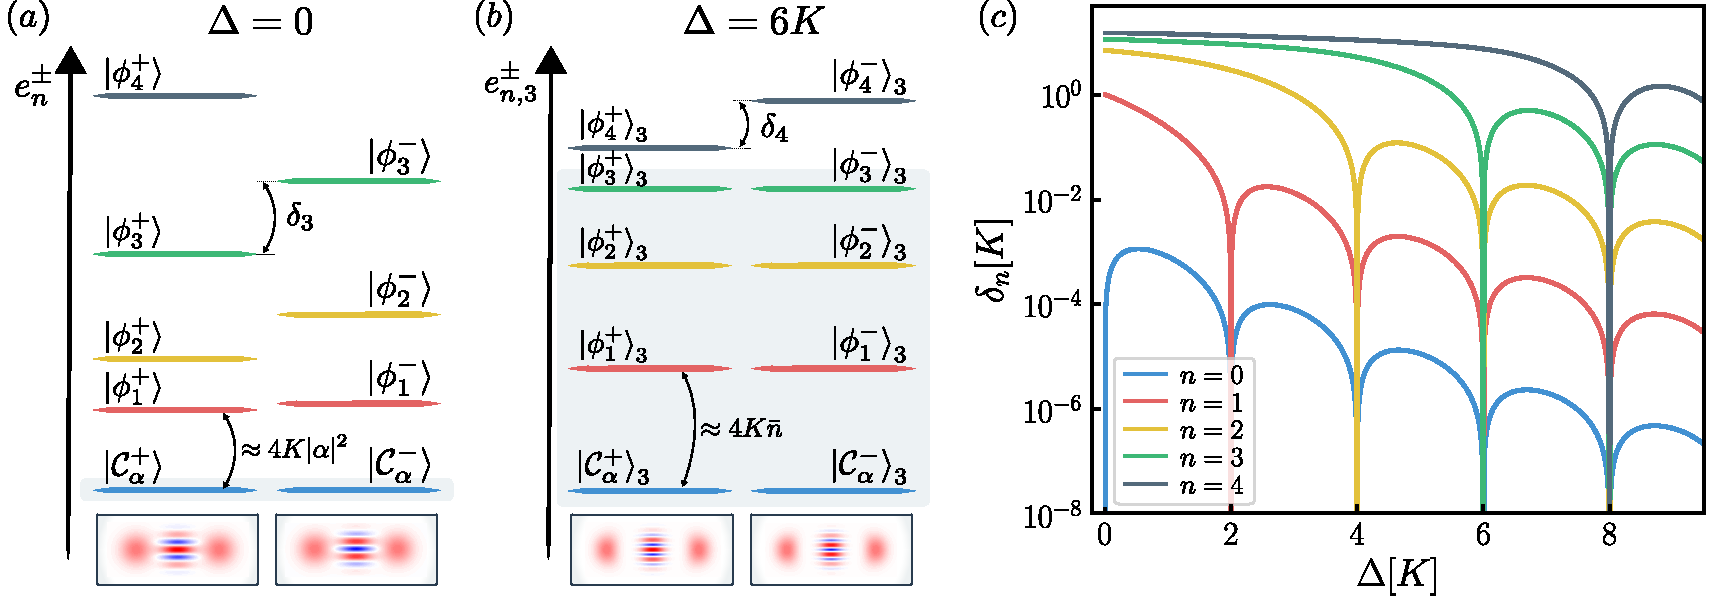
\includegraphics[width=\textwidth]{file/image/Spectre_V3.pdf}
    \vspace{-0.5cm}
    \caption{\label{fig:arche}
    (a) Energy levels of the Kerr Hamiltonian for $|\alpha|^2=4$, separated into two sets of even and odd photon-number parity states. The two ground states encode the cat qubits, protected by an energy gap $4 K |\alpha|^2$ from coherent perturbations. (b) Energy levels of the detuned Kerr Hamiltonian for $\Delta = 6K$ and $|\alpha|^2=\epsilon_2/K=4$. The first 4 pairs of eigenstates are exactly degenerate. The ground states are no longer cat states but are slightly deformed. Their mean photon number is given by $\bar n>|\alpha|^2$ for $\Delta>0$. (c) Spacing $\delta_n$ between the energy levels $\ket{\phi_n^+}$ and $\ket{\phi_n^-}$ for $|\alpha|^2=\epsilon_2/K=4$ as a function of the detuning $\Delta$. Both the energy level spacings and the detuning are in units of Kerr strength $K$. When $\Delta = 2mK$, the $2m+2$ first energy levels come in $m+1$ pairs of exactly degenerate states.
    }
\end{figure*}
%-------------------------------%

However, incoherent perturbations due for instance to thermal excitations or Markovian photon dephasing leak the cat states to higher excited states. For instance, thermal excitations leak $\ket{\alpha}$ into $\ket{\alpha,1} = \hat{D}(\alpha) \ket{1}$ up to first order, where $\hat{D}$ is the displacement operator, and $\ket{\alpha,1}$ has a non-zero overlap with all eigenstates $\{\ket{\phi_n^\pm}\}_{n \ge 1}$. These higher eigenstates come in nearly degenerate pairs but their non-degeneracy is enough to generate a rather fast dephasing between odd and even photon number parity subspaces. In the phase space picture, such dephasing can be seen as non-local excursions between left and right half planes. This ultimately breaks down the protection of the Kerr cat qubit against bit-flip errors.

In order to capture the above non-local excursions in phase space, let us consider the average value of the observable $\hat S=\text{sign}(\hat X)=\text{sign}(\hat a+\hat a^\dag)$,
\begin{equation}
    \bra{\psi}\hat S \ket{\psi}=\int_0^\infty |\psi(x)|^2dx-\int_{-\infty}^0 |\psi(x)|^2 dx. 
\end{equation}
Following the calculations of~\cite{Gautier2022}, starting from one of the cat-qubit computational states, the dynamics of $|\langle \hat S\rangle|$ is well approximated by $\exp(-\Gamma t)$, with
\begin{equation}
    \begin{split}
        \Gamma &= \kappa_1|\alpha|^2e^{-4|\alpha|^2} + \kappa_le^{-2|\alpha|^2} \\
        & \quad +\kappa_l\sum_{n>0} \lambda_n \left[ 1- \frac{\text{sin}(\delta_n/\kappa_{\text{conf}}
        )}{\delta_n/\kappa_{\text{conf}}} \right].
        \label{eq:formuleRonan}
    \end{split}
\end{equation}
Here, $\kappa_l$ is the rate of leakage outside of the manifold span$\{\ket{\mathcal{C}_\alpha^+},\ket{\mathcal{C}_\alpha^-}\}$. Typically, taking a thermal excitation rate $n_{\text{th}}\kappa_1$ ($\kappa_1$ denoting the relaxation rate of the harmonic oscillator), and possibly a Markovian photon dephasing rate of $\kappa_\phi$, the leakage rate is given by $\kappa_l=n_{\text{th}}\kappa_1+|\alpha|^2\kappa_\phi$. Furthermore, $\lambda_n$ denotes the average overlap between $\ket{\alpha,1}$ and the eigenstates of the driven Kerr Hamiltonian $\ket{\phi_n^\pm}$. It reads $\lambda_n=\sum_{\pm}|{\braket{\alpha,1}{\phi_n^\pm}}^2/2$. Finally, $\delta_n$ is the energy level spacing between $\ket{\phi_n^-}$ and $\ket{\phi_n^+}$, $\delta_n = e^-_n - e^+_n$, and $\kappa_\text{conf}$ the dissipative confinement rate of the cat manifold. In the absence of non-linear dissipative mechanisms~\cite{Mirrahimi2014} or colored dissipation~\cite{Putterman2022}, $\kappa_\text{conf}$ is simply given by $\kappa_1$, the energy relaxation rate of the harmonic oscillator.

The last term in Eq.~\eqref{eq:formuleRonan} highlights the contribution of each pair of nearly degenerate excited eigenstates to the non-local excursion, leading in term to bit-flip errors on the cat qubits. These excited pairs contribute to the bit-flip rate as soon as their energy-level spacing $\delta_n$ is significant with respect to $\kappa_{\text{conf}}$. For any $n$, the associated spacing $\delta_n$ converges to 0 when increasing the cat-qubit mean number of photons $|\alpha|^2$. This leads to a staircase pattern in the decreasing bit-flip error rate when increasing this mean number of photons. Such a behaviour was recently observed experimentally in a close concordance with theory~\cite{Frattini-2022}.  

Assuming now that the squeezing drive is detuned with respect to the Kerr resonator frequency, the  Hamiltonian in the drives rotating frame becomes 
\begin{equation}
    \begin{split}
        \hat{H}_\Delta &= K\hat{a}^{\dagger 2}\hat{a}^{ 2} + \epsilon_2 \hat{a}^{\dagger 2} + \epsilon_2^* \hat{a}^{2} - \Delta  \hat{a}^{\dag} \hat{a} \\
        &= K(\hat{a}^{\dagger 2} - \alpha^{*2})(\hat{a}^{ 2} - \alpha^2) - \Delta  \hat{a}^{\dag} \hat{a}
    \label{eq:DKerr}
    \end{split}
\end{equation}
where $\Delta$ is the detuning of the two-photon drive. Importantly, for $\Delta = 2mK$ with $m \in \mathbb{N}$ a positive integer, this Hamiltonian exhibits a bistable behaviour, \ie~two degenerate ground states~\cite{Roberts2019}. We denote the ground states of even photon-number parity by $\ket{\mathcal{C}_\alpha^+}_m$ or $\ket{+}_m$ and odd parity by $\ket{\mathcal{C}_\alpha^-}_m$ or $\ket{-}_m$, and define
\begin{equation}
    \begin{split}
        &\ket{0}_m=\frac{1}{\sqrt{2}}(\ket{\mathcal{C}_\alpha^+}_m+\ket{\mathcal{C}_\alpha^-}_m) \\
        &\ket{1}_m=\frac{1}{\sqrt{2}}(\ket{\mathcal{C}_\alpha^+}_m-\ket{\mathcal{C}_\alpha^-}_m).
        \label{newstates}
    \end{split}
\end{equation} 
Note that for $m \geq 1$, $\ket{0}_m$ and $\ket{1}_m$ are no longer coherent states, but they remain located on distinct parts of the phase plane. Figure~\ref{fig:wigner} shows the Wigner representation of $\ket{0}_m$ for increasing values of the detuning $\Delta$.

%-------------------------------%
\begin{figure}[t!]
    \centering
    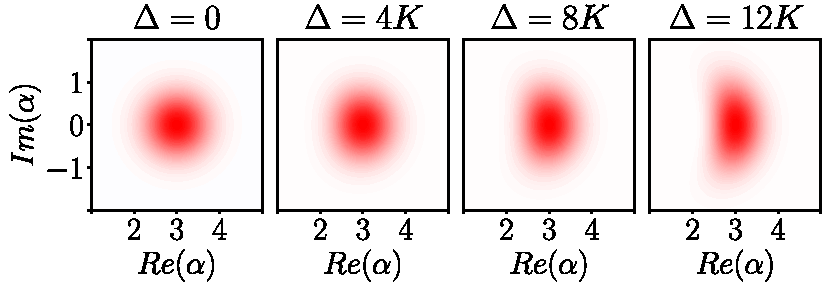
\includegraphics[width=\columnwidth]{file/image/Banane_V2.pdf}
    \vspace{-0.5cm}
    \caption{\label{fig:wigner}
    Wigner functions of the states $\ket{0}_{m}$ for $m=0,2,4,6$ and $\nbar = 9$. As $\Delta$ increases, the ground state of the detuned Kerr Hamiltonian is further distorted from a coherent state.}
\end{figure}
%-------------------------------%

Figure~\ref{fig:arche}(b) shows the eigenenergies of the Hamiltonian of Eq.~\eqref{eq:DKerr} for $m=3$. The Hamiltonian admits $m +1$  pairs of perfectly degenerate energy levels. We have grouped the higher eigenstates by their photon-number parity and denote them $\ket{\phi_n^\pm}_m$ with $e^\pm_{n,m}$ their respective energy. For $n \le m$, we denote by $\ket{\psi^0_n}_m$ and $\ket{\psi^1_n}_m$ the corresponding degenerate states located on the right- and left-hand side of phase space. They read
\begin{equation}
    \begin{split}
        &\ket{\psi^0_n}_m =\frac{1}{\sqrt{2}}\left(\ket{{\phi}_n^+}_m+\ket{{\phi}_n^-}_m\right) \\
        &\ket{\psi^1_n}_m =\frac{1}{\sqrt{2}}\left(\ket{{\phi}_n^+}_m-\ket{{\phi}_n^-}_m\right).
    \end{split}
\end{equation} 

Figure~\ref{fig:arche}(c) shows the energy level spacing $\delta_n$ between $\ket{{\phi}_n^+}$ and $\ket{{\phi}_n^-}$, as a function of the detuning. The combination of two mechanisms are thus demonstrated. As $\Delta$ increases, the mean number of photons in the cat states increases also because the frequency of the two-photon drive approaches the resonant frequency of higher transitions in the Kerr non-linear oscillator. Thus the energy level spacing $\delta_n$ between $\ket{{\phi}_n^+}$ and $\ket{{\phi}_n^-}$ diminishes as it does when the strength of the two-photon drive $|\epsilon_2|$ increases. For $\Delta = 2mK$ with $m \in \mathbb{N}$, the two-photon drive frequency becomes resonant with the transition $\ket{m}$ to $\ket{m+1}$ of the Kerr non-linear oscillator. As shown by the peaks around $\Delta~=~2mK$, new bistability points appear that include more and more pairs of degenerate eigenstates as $\Delta$ increases. We can also note that the energy gap increases between the first and second pair of degenerate eigenstates when $\Delta$ increases, as it does when $|\epsilon_2|$ increases. For the rest of this paper, we will use $|\alpha|^2 = |\epsilon_2/K|$ and $\bar{n} = \expval{a^\dagger a}$. Note that $\bar{n} \ne |\alpha|^2$ for $\Delta >0$ but rather $\bar{n} \approx |\epsilon_2/K|+\Delta/(2K)$ because the detuning increases the number of photons in the cavity. As it will become more clear in the next section, and according to Eq.~\eqref{eq:formuleRonan}, this is of particular interest to have multiple degenerate states in the spectrum, since the first $m +1$ pairs of eigenstates will not contribute to bit-flip errors.

We conclude this section by noting that for the particular choices of detuning $\Delta=2mK$, the $m +1$ pairs of degenerate eigenstates can be calculated analytically by diagonalizing two matrices of dimension $m+1$. In what follows, we assume that $\alpha$ is real. The first step is to displace the detuned Kerr Hamiltonian by~$\pm \alpha$
\begin{equation*}
    \begin{split}
        \tilde{H}_\pm &= \hat D(\pm \alpha) \hat{H}_\Delta \hat D(\mp \alpha) \\
         &= K \left( \adagsq \mp 2 \alpha \hat{a}^{\dagger} \right) \left( \hata^2 \mp 2 \alpha \hata \right) -  \Delta (\hat{a}^{\dagger} \mp\alpha)( \hata \mp \alpha)
    \end{split}
\end{equation*}
where $\hat D$ denotes the displacement operator. Evaluating this displaced frame Hamiltonian on the $n$-th Fock state $\ket{n}$ yields
\begin{equation}
    \begin{split}
        \tilde{H}_\pm \ket{n} & = \left[K (n-1) + 4 K |\alpha|^2 - \Delta \right] n \ket{n} \\ 
        & \mp \left[2K n - \Delta \right] \alpha \sqrt{n+1} \ket{n+1} \\
        & \mp \left[2K (n-1)  - \Delta \right] \alpha \sqrt{n} \ket{n-1}
    \end{split}
\end{equation}
For $\Delta = 2mK$, the Hamiltonians $\tilde H_\pm$ map the finite-dimensional Hilbert space spanned by the first $m+1$ Fock states to itself. In other words, these Hamiltonians are block diagonals. Therefore, by diagonalizing the associated block matrices of dimension $(m+1)\times(m+1)$, we can calculate the $(2m+2)$ first eigenstates of the Hamiltonian $\hat H_\Delta$, as being their displacements by $\mp\alpha$.  For instance for $m=1$, this leads to
\begin{equation*}
    \begin{split}
        \ket{0}_{m=1} &= \text{cos}(\theta)\ket{\alpha} + \text{sin}(\theta) \ket{\alpha,1} \\
        \ket{{1}}_{m=1} &= \text{cos}(\theta)\ket{-\alpha} - \text{sin}(\theta) \ket{-\alpha,1} \\
        \ket{\psi^0_{1}}_{m=1} &= \text{sin}(\theta)\ket{\alpha} - \text{cos}(\theta) \ket{\alpha,1} \\
        \ket{\psi^1_{1}}_{m=1} &= \text{sin}(\theta)\ket{-\alpha} + \text{cos}(\theta) \ket{-\alpha,1} \\
    \end{split}
\end{equation*}
with
\begin{equation*}
\theta=\arctan\left(\frac{2|\alpha|}{2|\alpha|^2-1+\sqrt{4|\alpha|^4+1}}\right).
\end{equation*}
Furthermore the eigenenergies corresponding to each pair are perfectly degenerate and the energy gap between the ground and first excited subspaces is given by
\begin{equation}
    \begin{split}
        e^\pm_{1,1}-e^\pm_{0,1}  &= 2 K \sqrt{1+4|\alpha|^4}.
    \end{split}
\end{equation}

For $\Delta = 2Km, m > 1 $ we have
\begin{equation*}
    \begin{split}
        \ket{\psi^0_n}_m &= \sum_{j=0}^{m} c_{m,n,j}(\alpha) \ket{\alpha,j} \\
        \ket{\psi^1_n}_m &= \sum_{j=0}^{m} c_{m,n,j}(-\alpha) \ket{-\alpha,j} \\
        &= \sum_{j=0}^{m} (-1)^{m+j} c_{m,n,j}(-\alpha) \ket{-\alpha,j}
    \end{split}
\end{equation*}
where $c_{m,n,j}(\alpha)$ and the respective eigenenergies depend on the $\text{n}^\text{th}$ square root of a polynomial of degree $m+1$.

\section{\label{sec:level4}Phase space confinement}

In the previous section, we argued that the slow suppression of bit-flip errors in resonant Kerr cat qubits can be explained through the non-degeneracy of excited energy-level pairs in the driven Kerr Hamiltonian. We also saw that, for specific choices of detuning $\Delta \in 2K\mathbb{N}$, the detuned Kerr Hamiltonian remarkably admits $m+1$ pairs of perfectly degenerate eigenstates. One can guess that this change in the spectrum should drastically improve the phase space confinement, and therefore lead to a faster suppression of induced bit-flip errors. To quantify this phase space confinement, we look at the average value of the observable $\hat S=\text{sign}(\hat X)=\text{sign}(\hat a+\hat a^\dag)$. This observable is very close to the two-photon dissipation conserved quantity $J_X=J_{+-}+J_{-+}$ defined in~\cite{Mirrahimi2014}, and quantifies whether the state of the oscillator state is located in the right or left half plane of phase space.  

The simulations were performed as follows. We initialize the system in the state $\ket{0}{\bra{0}}_m$ and let it evolve under the master equation 
\begin{equation}
    \dot{\hat\rho} = -i [\hat H_\Delta,\hat \rho] + \kappa_- \mathcal{\hat D}[\hata]\hat \rho + \kappa_+ \mathcal{\hat D}[\hat{a}^{\dagger}]\hat \rho + \kappa_\phi \mathcal{\hat D}[\hat{a}^{\dagger} \hata]\hat \rho
\end{equation}
where $\kappa_- = \kappa_1 (1 + n_{\text{th}})$, $\kappa_+ = \kappa_1 n_{\text{th}}$, $\kappa_1$ is the single-photon loss rate, $n_{\text{th}}$ is the thermal population and $\kappa_\phi$ is the dephasing rate. The excursions in phase space are quantified by $\langle \hat S \rangle_t = \Tr\bigl[\hat S\hat\rho(t)\bigr]$. By simulating the system over a long time of order $T=100/\kappa_1$, we can fit the above quantity $\langle \hat S\rangle_t$ to a single exponential $\exp(-2\Gamma_S t)$. For a strongly confined system, the above excursion rate $\Gamma_S$ will be very small.  The numerical simulations were performed in the basis of Kerr eigenstates with a truncation to 20 eigenstates.

Figure~\ref{fig:bitflip} presents such simulations for $\kappa_1 = 10^{-3}K,n_{\text{th}} = 10^{-2} \text{ and } \kappa_\phi = 10^{-5}K$. The rate $\Gamma_S$ is evaluated as a function of $\bar{n} = \expval{\hat{a}^{\dagger} \hata}$. We remind that $\bar{n} > |\epsilon_2/K|$ for $\Delta>0$. As expected, we benefit from a much stronger phase space confinement for $\Delta = 2mK$, $m \ge 1$ compared to $\Delta = 0$. Note however that for a fixed low $\bar{n}$, the phase space excursions can be faster when increasing $\Delta$. This is mainly due to the fact that for large $\Delta$, the two-photon drive amplitude $|\epsilon_2|$ becomes too weak to separate the states $\ket{0}_m$ and $\ket{1}_m$ in phase space.  More precisely, for a fixed $\bar{n}$, an optimal $\Delta$ can be found to minimize the excursion rate $\Gamma_S$: $\Delta_{opt} \approx \nbar K$. Furthermore, this optimized rate $\Gamma_S$ scales as $e^{-\gamma\bar{n}}$ with $\gamma \approx 0.65$ (dashed line in Fig.~\ref{fig:bitflip}).


%-------------------------------%
\begin{figure}[t!]
    \centering
    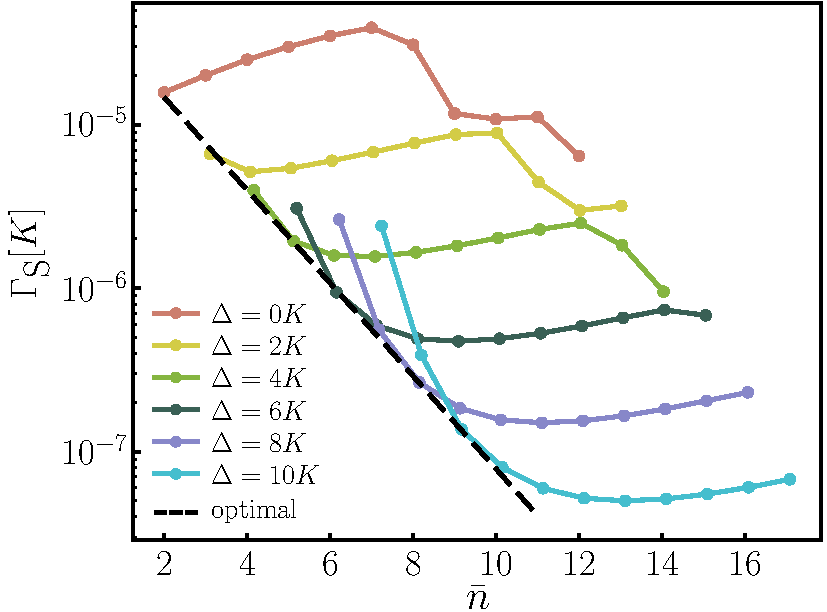
\includegraphics[width=\columnwidth]{file/image/Bitflip_V2.pdf}
    \vspace{-0.5cm}
    \caption{\label{fig:bitflip}
         Phase space excursion rate $\Gamma_\text{S}$, \ie~rate at which the expectation value $\langle \hat S \rangle$ of the confinement observable $\hat S=\textrm{sign}(\hata+\hat{a}^{\dagger})$ decays to zero. This rate is plotted as a function of $\bar{n} = \langle\hat{a}^{\dagger} \hata\rangle$ for $\kappa_1 = 10^{-3}K$, $n_{\text{th}}=10^{-2}$ and $\kappa_\phi = 10^{-5}K$ and  for different detuning values. As $\Delta=2mK$ increases, more and more eigenstates come in degenerate pairs and do not contribute to such phase space excursions. Thus the rate $\Gamma_S$ decreases and saturates at a lower value when increasing $\bar n$. For a fixed value of $\bar n$, however, there is an optimal choice of $\Delta$ that minimizes the rate $\Gamma_S$: $\Delta_{\text{opt}} \approx \nbar K$. The associated optimal rate $\Gamma^{\text{opt}}_S$ scales as $e^{-\gamma\bar n}$, with $\gamma\approx 0.65$ (note that this value corresponds to the specific values of $\kappa_1,n_{\text{th}} \text{ and } \kappa_\phi$ chosen).
    }
\end{figure}
%-------------------------------%

The Kerr cat, on resonance or detuned, undergoes an important amount of leakage due to thermal excitation and dephasing, as can be seen on Fig.~\ref{fig:thermalstate}(a), (b) and (c) with the red bar charts. The situation is however different when the system is only subject to  single-photon loss. In this case, the resonant Kerr cat has a very small leakage because the coherent states are not affected by the annihilation operator $\hata$. However the detuned Kerr cat states are no longer perfect eigenstates of  $\hata$. Thus, the single-photon loss induces significant leakage to the other energy levels. 

On Fig.~\ref{fig:thermalstate}(a), (b) and (c), the blue bar charts represent the population on the $n$-th pair of eigenstates when the detuned Kerr cat is only undergoing single-photon loss and has reached a steady state. As it can be seen in these charts, the single-photon loss only induces leakage to the eigenstates in the degenerate part of the spectrum. Indeed, for the detuned Kerr cats, because the manifold Span$\{{\ket{\psi^0_n}}_m\}_{n\in  [\![ 0,m]\!]}$ is equal to the manifold Span$\{{\ket{\alpha,n}}\}_{n\in  [\![ 0,m]\!]}$, which is stable under the application of $\hata$, single-photon loss only populates the degenerate pairs of eigenstates. Interestingly, as it can be seen in plots (b) and (c), this degenerate manifold reaches a mixed state with an  exponential distribution on degenerate pairs close to a thermal state distribution with an effective non-zero temperature.  Figure~\ref{fig:thermalstate}(d) shows the effective mean number of excitations $\bar n_{ex}$ in this degenerate manifold. In particular, we see that it increases very rapidly with $\Delta$. Note that this mean excitation number does not depend on $\kappa_1$. In order to work with well defined qubits for fault-tolerant quantum computation, this leakage needs to be suppressed. This can be done through the addition of dissipative processes refocusing the population to the ground manifold of the detuned Kerr Hamiltonian. 

%-------------------------------%
\begin{figure}[t!]
    \centering
    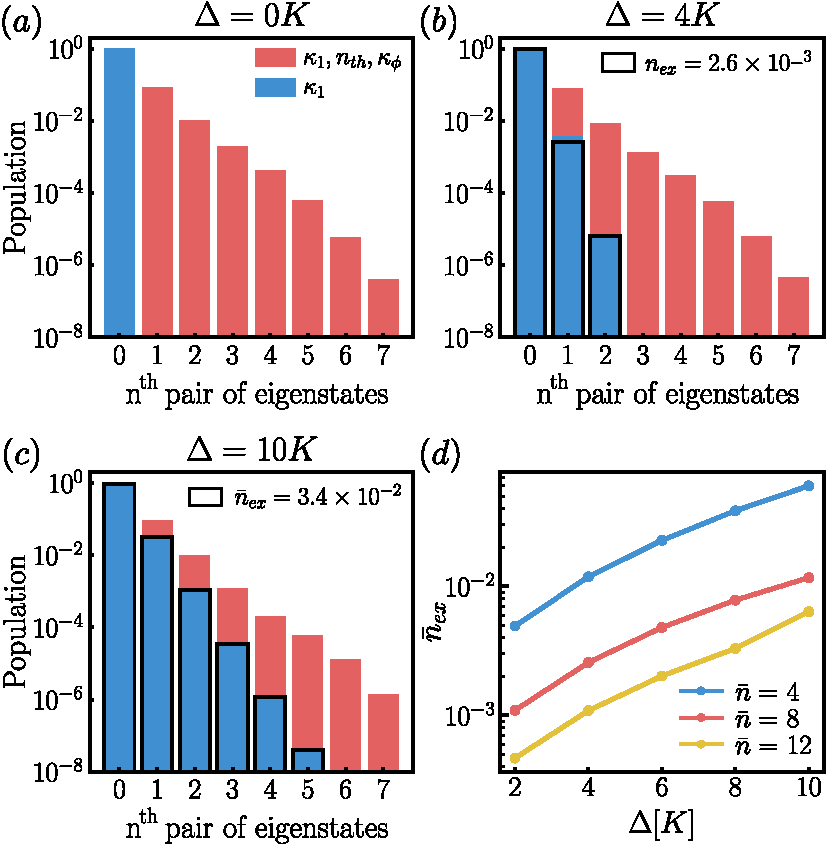
\includegraphics[width=\columnwidth]{file/image/thermal_state_V2.pdf}
    \vspace{-0.5cm}
    \caption{\label{fig:thermalstate}
    Steady state population of the eigenstates of the detuned Kerr Hamiltonian for (a) $\Delta = 0K$, (b) $\Delta = 4K$ and (c) $\Delta = 10K$, and for $\nbar = 10$, $\kappa_1 = 10^{-3}K$, $n_{\text{th}}=10^{-2}$ and $\kappa_\phi = 10^{-5}K$. Starting from $\ket{0}_m$, a time of the order of $1/\kappa_1$ is needed to reach this mixed steady state. In presence of thermal excitation or dephasing, all eigenstates are populated following an exponential distribution that does not significantly change with the detuning. However, under the absence of these processes, and thus under the sole effect of single-photon loss channel, only the degenerate pairs are populated. In the latter case, the populations of these degenerate eigenstates reach a distribution close to the Boltzmann distribution of a thermal state. (d) The effective mean number of excitations $\bar n_{ex}$ of the mixed steady state of the driven detuned Kerr under single-photon loss as a function of the detuning and for different values of $\nbar$. 
    }
\end{figure}
%-------------------------------%


\section{\label{sec:colored}Detuned Kerr cats with colored dissipation}

Bosonic qubits are often solely defined through their codespace, which is a two-dimensional subspace of an oscillator infinite-dimensional Hilbert space. However, a full definition of bosonic qubits should include a complete mapping from the oscillator space to this code space to characterize any leakage that may occur outside of it. Indeed, once readout of the bosonic qubit is performed, it is important to be able to associate any potential leakage out of codespace to one of the qubit computational states. For instance, in the case of GKP qubits~\cite{Gottesman2001,CampagneIbarcq2020}, the full oscillator space is mapped to the qubit through a grid-like separation of phase space. Any small displacement away from the codespace would thus be properly taken into account.

For cat qubits, such a mapping can be performed with dissipative stabilization by associating any initial state to its infinite-time steady state once reconverged to the cat-qubit codespace. As such, it is essential to have a process that eliminates leakage in order to rigorously define cat qubits. For the detuned Kerr cat qubit introduced in this paper, this dissipative stabilization cannot be realized with the driven two-photon dissipation $\mathcal{D}[\hat{a}^2 - \alpha^2]$ as the ground states of the Hamiltonian are not coherent states anymore, thus are not dark states of this dissipative super-operator. Instead, we show in this section that the stabilization of detuned Kerr cat qubits may be achieved with a colored dissipation.

The colored dissipation method introduced in Ref.~\cite{Putterman2022} consists in enabling precise frequency decays to bring back leakage to the ground eigenspace of the detuned Kerr Hamiltonian. The full system can be modelled as follows,
\begin{equation}
    \begin{split}
        \frac{d \hat \rho}{dt} &= -i[\hat H_\Delta + \hat H_\text{color},\hat \rho] + \kappa_1(1+n_{\text{th}}) \mathcal{\hat D}[\hat a]\hat \rho \\ 
        & + \kappa_1 n_{\text{th}} \mathcal{\hat D}[\hat{a}^{\dagger}]\hat \rho + \kappa_\phi \mathcal{\hat D}[\hat{a}^{\dagger} \hata]\hat \rho + \kappa_f \mathcal{\hat D}[\hat f_M]\hat \rho
        \label{eq:color}
    \end{split}
\end{equation}
where
\begin{equation}
        \hat H_\text{color} = g \hat a \hat f_1^\dagger e^{i\Delta_f t} + J \sum_{j=1}^{M-1}\hat f_j \hat f_{j+1}^\dagger + \hc
\end{equation}
is an interaction Hamiltonian between the Kerr cat mode $\hata$ and all filter modes $\hat f_1,...,\hat f_{M}$, with respective frequencies $\omega_a$ and $\omega_f$. Together with the dissipation of the last filter mode in $\mathcal{D}[\hat{f}_M]$, this Hamiltonian approximates an ideal band-pass filter centered on the  frequency $\omega_f=\omega_a+\Delta_f$, with half bandwidth $\kappa_f = 2J$ ~\cite{Putterman2022}.

The main point of this filter is to allow the relaxations $\ket{\phi_n^\pm}_m \rightarrow \ket{\phi_{n-1}^\mp}_m$ to occur, thus countering the leakage from the code space, while filtering out the transitions $\ket{\phi_n^\pm}_m \rightarrow \ket{\phi_n^\mp}_m$ that solely induce photon number parity jumps without reducing state leakage. Indeed, while the first kind of transition features an energy difference $\Delta_f \gtrsim 4K \nbar$, the second kind has a typical energy difference $\Delta_f \approx 0$, where the equality is verified within the exactly-degenerate subspace of the detuned Kerr Hamiltonian (see Fig.~\ref{fig:arche}(b)). Note in particular that all of these transitions swap the cat state parity, thus leakage elimination with colored dissipation is performed while inducing parity swaps. This is beneficial for certain gates, as it ensures the correction of first-order non-adiabatic phase-flip errors (see Ref.~\cite{Putterman2022} for details).

Similarly as in Ref.~\cite{Putterman2022}, we set the filter detuning frequency at the first excited to ground state transition frequency, \ie~$\Delta_f \approx 4K \bar{n}$. We also set $\kappa_f = 2J = \Delta_f / 5$ and $g = \kappa_f / 5$ like for the regular colored Kerr cat, such that adiabatic elimination of the ancillary filter modes can be performed. In the limit of a large number of filter modes, this colored dissipation leads to an engineered dissipation rate $\kappa_{1,\textrm{eng}}=4g^2/\kappa_f$. A notable difficulty in the design of this system is to filter out the $\Delta_f \approx 0$ transitions --- in order not to induce persistent phase-flip errors --- while maintaining a maximum number of higher energy transitions. As such, it may be relevant to feature multiple band-pass filters at various transition frequencies, so-called "colors".

The population of the steady state of the detuned Kerr cat is shown in Fig.~\ref{fig:coloredthermalstate}(a), with (blue) or without (red) colored dissipation and for a fixed detuning $\Delta = 10K$, cat size $\nbar = 10$, in presence of several leakage-inducing dissipative terms such as thermal excitation and dephasing. Several orders of magnitude of reduction in the amount of leakage are therefore demonstrated once this colored dissipation is added. In particular, the rate of this colored dissipation, or the number of colors, can be adjusted to further reduce leakage. The leakage reduction induced by colored dissipation is shown in Fig.~\ref{fig:coloredthermalstate}(b) as a function of the mean number of photons $\bar{n}$ and for different values of the detuning $\Delta$.

%-------------------------------%
\begin{figure}[t!]
    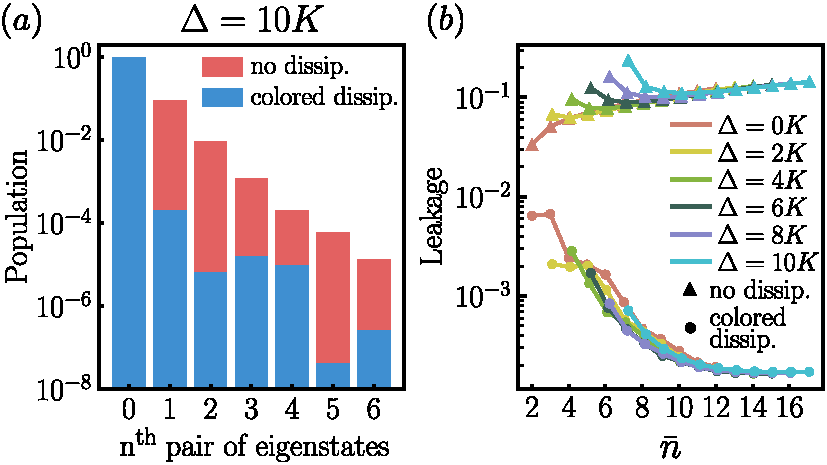
\includegraphics[width=\columnwidth]{file/image/Color_Thermal_State_V2.pdf}
    \caption{\label{fig:coloredthermalstate}
    (a) Thermal Population of the eigenstates of the detuned Kerr Hamiltonian for $\Delta = 10K$ for $\nbar = 10,\kappa_1 = 10^{-3}K, n_{\text{th}}=10^{-2},$ and $\kappa_\phi = 10^{-5}K$ without colored dissipation (in red) and with colored dissipation (in red). The colored dissipation reduces the leakage by nearly three orders of magnitudes. (b) Leakage out of the code space as a function of $\nbar$ and for different values of $\Delta$. The colored dissipation works regardless of the value of the detuning.
    }
\end{figure}
%-------------------------------%


Once a dissipative scheme stabilizing the two-dimensional subspace (preventing state leakage to accumulate) is precised, we may speak of a well defined qubit. The logical Pauli operators of the cat qubit are defined as $Z=\text{sign}(\hata+\hat{a}^{\dagger})$ and $X=\exp(i\pi\hat{a}^{\dagger}\hata)$. Note that, by reducing leakage, the colored dissipation also reduces the bit-flip rate. This can be seen from the rate of phase space excursions $\Gamma_S$ that now corresponds to the bit-flip error rate $\Gamma_\text{bit-flip}$. Similar simulations to those performed in the previous Section, but now in the presence of colored dissipation, are provided in Fig.~\ref{fig:coloredbitflip}. In these simulations, we let the system evolve from the state $\ket{0}_m$ under the master equation~\eqref{eq:color} for a time of order $10/\kappa_1$, and fit $\expval{Z}_t=\langle \hat S \rangle_t$ to an exponential $\exp(-2\Gamma_{\text{bit-flip}}t)$. Figure~\ref{fig:coloredbitflip}(a) shows the resulting bit-flip error rates for different values of $\bar{n}$ and detuning, with $\kappa_1 = 10^{-3}K$, $n_{\text{th}} = 10^{-2}$ and $\kappa_\phi = 10^{-5}K$. The simulations were performed in the Kerr eigenstate basis with a truncation of 14 eigenstates. Following Ref.~\cite{Putterman2022}, we assume that there is at most one photon in all $N$ filter modes, such that they can all be simulated at once using a Hilbert space of dimension $N+1$.

Note that for a small number of filter modes, the addition of colored dissipation can induce additional phase-flip errors. Thus, in practice, a certain number of modes are needed so that the additional phase-flip errors become negligible compared to those caused by the intrinsic single-photon loss. For the parameters in our simulations, this level of filtering is reached using three modes. In practice, one might want to reduce the engineered colored dissipation rate $\kappa_{1,eng}$, in order to avoid further phase-flip errors due to the absence of a perfect cut-off, or to limit the non-adiabatic gate errors introduced in the next section. Increasing the detuning enables to reach an equivalent bit-flip error rate, but for a weaker colored dissipation rate.

%-------------------------------%
\begin{figure}[t!]
    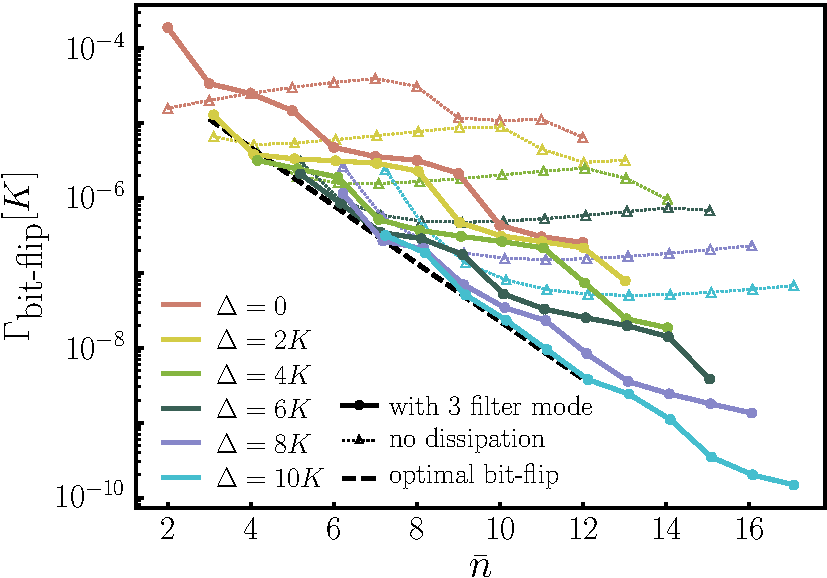
\includegraphics[width=\columnwidth]{file/image/Color_Bitflip_V2.pdf}
    \vspace{-0.5cm}
    \caption{\label{fig:coloredbitflip} 
    Bit-flip error rate as a function of $\nbar$ for different values of the detuning $\Delta$ and for $\kappa_1 = 10^{-3}K, n_{\text{th}}=10^{-2}$ and $\kappa_\phi = 10^{-5}K$. The transparent curves represent the phase space excursion rate without colored dissipation (same as Fig.~\ref{fig:bitflip}), and the plain curves represent the bit-flip rate with colored dissipation. For a fixed value of $\bar n$, there is an optimal choice of $\Delta$ that minimizes the rate $\Gamma_\text{bit-flip}$. The associated optimal rate $\Gamma^{\text{opt}}_\text{bit-flip}$ scales as $e^{-\gamma\bar n}$, with $\gamma\approx 0.89$ (note that this value corresponds to the specific values of $\kappa_1,n_{\text{th}} \text{ and } \kappa_\phi$ chosen).
    }
\end{figure}
%-------------------------------%

\section{\label{sec:level6}Bias-preserving gates}

For a universal set of logical operations, it is required to be able to prepare cat states in both $\ket{0}_c$ and $\ket{+}_c$~\cite{Guillaud2019}. The preparation of $\ket{+}_c$ can be achieved by adiabatically increasing both the two-photon drive strength and detuning. The best adiabatic path can be optimized in a similar way as Ref.~\cite{Yanagimoto2019} leading to a preparation analogous to on-resonance Kerr cats. The preparation of $\ket{0}_m$ can be achieved similarly, starting from a coherent state stabilized with an on-resonance Kerr Hamiltonian, and adiabatically increasing the detuning. During this preparation, the rate of bit-flip errors will be equivalent to the on-resonance Kerr, and will then recover the rate described in Fig.~\ref{fig:coloredbitflip}.

The implementation of bias-preserving gates on cat qubits, as required for a universal set of fault-tolerant logical gates, are achieved using two types of dynamics, so-called Zeno and topological gates~\cite{Mirrahimi2014,Guillaud2019,Puri2020}. A Zeno gate typically makes use of the quantum Zeno effect to perform a rotation of an arbitrary angle $\theta$ around the Z axis by applying a weak near-resonant drive. In the rotating frame of the two-photon drive, such a Zeno gate can be modelled by the addition of the Hamiltonian 
\begin{equation}
    \hat H_Z(t) = \epsilon_Z(t) (\hat a^\dagger + \hat a)
    \label{eq:Z}
\end{equation}
to Eq.~\eqref{eq:DKerr}. Here, $\epsilon_Z(t)$ represents a slowly varying modulation of the driving field amplitude. A rotation around the Z axis of the Bloch sphere is then realized with an angle $4 \sqrt{\nbar} \int_0^T \epsilon_Z(t) dt$, where T is the duration of the gate. Accelerating such a gate usually comes at the expense of additional leakage out of the cat-qubit subspace due to non-adiabatic effects. In the absence of decoherence, and by benefiting from the adiabatic theorem with exponential accuracy~\cite{teufel:book}, it is possible to engineer pulses $\epsilon_Z(t)$ where these higher-order effects are carefully suppressed, thus reaching extremely fast gates~\cite{Xu2021}. Two-qubit entangling gates (rotations around $ZZ$ axis) can be performed in a similar manner~\cite{Mirrahimi2014}. These gates rely on the protection provided by the Hamiltonian gap and thus straightforwardly used in the context of detuned Kerr cats, while preserving the better scaling of bit-flip type errors.

We can distinguish two sources of phase-flip errors when applying such a Zeno gate. The first one corresponds to those induced by the undesired single-photon loss, with probability $p_Z = \nbar \kappa_1 T$. The second one is non-adiabatic errors, with probability $p_Z^{NA}$, which are created because the gate induces leakage out of the code space, and consequently this leakage is mapped to code space  errors after being removed by the engineered dissipation process. Without dissipation, the non-adiabatic errors can be exponentially suppressed with the gate duration, using the super-adiabatic pulse designs~\cite{Xu2021}. However, when combined with colored dissipation, the Z rotation induces further non-adiabatic errors. The detuned Kerr cats suffer from these non-adiabatic errors just as the resonant ones. However, for the same bit-flip error rate, the strength of the colored dissipation of the detuned Kerr cats can be reduced compared to the resonant ones, leading therefore to smaller non-adiabatic error rates. For instance, as can be seen on Fig.~\ref{fig:coloredbitflip}, at $\nbar = 8$ and for $\Delta = 10K$, the bit-flip rate of the detuned Kerr cats (even without colored dissipation) is smaller than the bit-flip rate of the resonant one with colored dissipation. Note however that the colored dissipation is still needed to counter leakage, and to work with well defined qubits. Figure~\ref{fig:Zgate} shows the reduction in non-adiabatic errors on a Z gate when reducing the strength of the colored dissipation from $\kappa_{1,eng}=K$ to $\kappa_{1,eng}=K/10$. 



The topological gates are based on a deformation of the code space. Typically,  a Pauli X gate is performed through a $\pi$-rotation of the phase space by rotating the two states confined by the Kerr dynamics $\ket{\alpha(t)} = \ket{\alpha e^{i \theta(t)}}$ (with $\theta(T)=\pi$), while applying a so-called feed-forward Hamiltonian ${\hat H(t)=-\dot\theta(t) \hat a^\dagger \hat a}$. Here, nothing in the dynamics is specific to having coherent states as confined states, and therefore the Pauli X gate can be implemented in the exact same manner for the detuned Kerr cats. Less trivially, the CNOT gate introduced in~\cite{Puri2020} can also be adapted to the detuned Kerr cats. It consists in rotating the confinement of the target qubit conditionally on the state of the control qubit as well as applying a CNOT feed-forward Hamiltonian
\begin{equation}
    \begin{split}
        &\hat H(t) = K(\hat{a}^{\dagger}sq_c - \alpha_c^2)(\hata^2_c - \alpha_c^2) - \Delta \hat{a}^{\dagger}_c \hata_c - \Delta \hat{a}^{\dagger}_t \hata_t \\
        &+ K\left[\hat{a}^{\dagger}sq_t - \alpha^2_t e^{-2 i \theta(t)} \left(\frac{\tilde{\alpha}_c - \hat{a}^{\dagger}_c}{2\tilde \alpha_c}\right) - \alpha_t^2 \left(\frac{\tilde{\alpha}_c + \hat{a}^{\dagger}_c}{2\tilde\alpha_c}\right) \right] \\ 
        &\times \left[\hata^2_t  - \alpha^2_t e^{-2 i \theta(t)} \left(\frac{\tilde{\alpha}_c - \hata_c}{2\tilde\alpha_c}\right) - \alpha_t^2 \left(\frac{\tilde{\alpha}_c + \hata_c}{2\tilde\alpha_c}\right) \right] \\
        &+ \dot\theta(t) \frac{2 \tilde{\alpha}_c - \hat{a}^{\dagger}_c - \hata_c}{4 \tilde\alpha_c} \otimes (\hat{a}^{\dagger}_t \hata_t - \nbar_t) 
        \label{eq:cnot-drive}
    \end{split}
\end{equation}
with
\begin{equation}
        \alpha = \sqrt{\varepsilon_2/K}, \quad
        \tilde{\alpha} = {\bra{0}}_m(\hat{a}^{\dagger}+\hata)\ket{0}_m/2,
\end{equation}
where $\Delta=2mK$, $\theta(T) = \pi$ and $\hata_c$ and $\hata_t$ are the annihilation operators of the control and target modes respectively. 

%-------------------------------%
\begin{figure}[t!]
    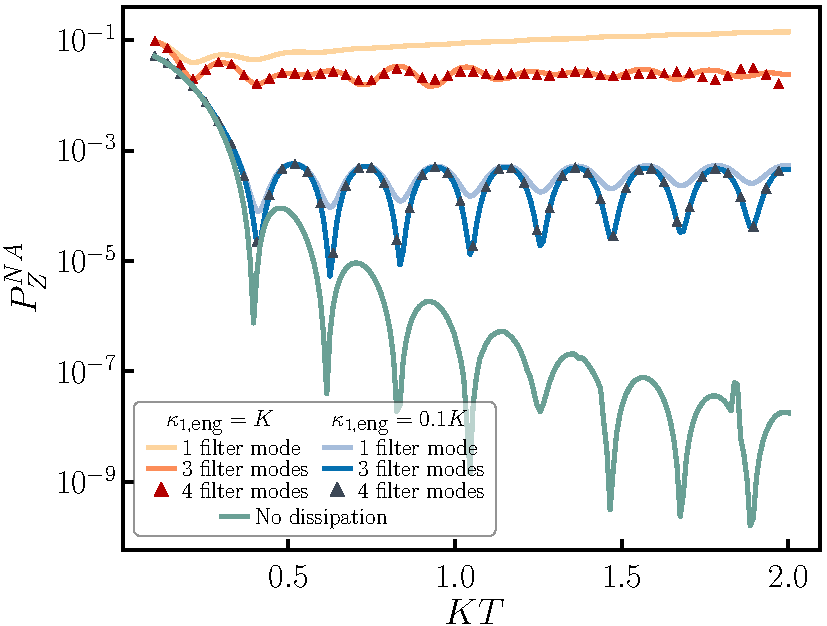
\includegraphics[width=\columnwidth]{file/image/Zgate_V2.pdf}
    \vspace{-0.6cm}
    \caption{\label{fig:Zgate}
    Non-adiabatic error probability $p_Z^{NA}$ for a Zeno $\pi$-rotation around the $Z$ axis, realized with a Gaussian pulse $\epsilon_Z(t)$ for $\nbar = 8$. Here $T$ is the gate duration and is expressed in units of $1/K$. Without dissipation, the non-adiabatic error probability can be reduced to as low as $10^{-8}$ for gate times of order $1/K$. But, with colored dissipation of strength $\kappa_{1,eng} = K$ such non-adiabatic error probability saturates above $10^{-2}$. Dividing by 10 the colored dissipation amplitude reduces the non-adiabatic error probability by approximately two orders of magnitudes. $p_Z^{NA}$ is also plotted for different number of filter modes in the colored dissipation, showing that it is not necessary to consider more than 3 filter modes here.
    }
\end{figure}
%-------------------------------%


\section{\label{sec:level9}Conclusion}

On the path towards a fault-tolerant quantum processor, biased-noise qubits are promising candidates as they significantly reduce the required overhead for error correction. By focusing on the case of Kerr cat qubits~\cite{Puri2017,Grimm2020,Frattini-2022}, we show in this paper that an extra control parameter, the detuning of the the two-photon drive with respect to the Kerr oscillator's resonance, plays a central role in the structure of the spectrum of the confinement Hamiltonian. For particular choices of detuning given by even multiples of the Kerr strength, not only the two encoding qubit states are perfectly degenerate, but also the excited states come in perfectly degenerate pairs. This strong symmetry significantly contributes to the properties of the encoded qubits. By keeping the information well confined in the left and right half planes of the phase space, such a degenerate spectrum strongly suppresses the phase space excursions induced by leakage mechanisms such as photon loss, thermal excitation, or photon dephasing. This Hamiltonian confinement can then be safely combined with a colored dissipation process countering the leakage and therefore leading to well-defined qubits. The degeneracy of the spectrum ensures that even a weak engineered dissipation is enough to benefit from a strong suppression of bit-flip errors. The weakness of the required dissipation provides room for engineering fast high-fidelity bias-preserving gates, where the information is not lost through the engineered dissipation channel. 

The analysis presented in this work is based on the effective static Hamiltonian given in equation~(\ref{eq:DKerr}). One may legitimately wonder whether this model is reasonable or not. Indeed, within this effective theory, it would seem that arbitrarily increasing the detuning of the squeezing drive would result in an arbitrary number of pairs of excited states being perfectly degenerate. In practice however, a number of approximations have been made to obtain this effective dynamics; and it would be interesting to investigate how higher order terms in the rotating wave approximation (RWA) affect the benefits of the perfect degeneracy of the eigenstates, or to derive a more general theory including beyond RWA effects, following the recent works of Refs.~\cite{Venkatraman2022}. However, even though the theory in this paper does not include the study of such effects, during the writing of this paper we have been informed that the experimental observations by our colleagues at Yale University~\cite{RodrigoExperiment} confirm the improvement of phase-space confinement property for specific detuning values mentioned in our paper.


\begin{acknowledgments}
D.R would like to thank Yiwen Chu for her supervision on this project. All the authors would like to thank Rodrigo Cortiñas, Raphaël Lescanne, Paul Magnard and Nathanaël Cottet for many enlightening conversations about the possible experimental realizations of this proposal. 
\end{acknowledgments}

%%%%%%%%%%%%%%%%%%%%%%%%%%%%%%%%
% APPENDICES
%%%%%%%%%%%%%%%%%%%%%%%%%%%%%%%%



\newpage
\appendix

\section{\label{sec:appendixA}Bit-flip simulation technique}

Bit-flip simulations were performed starting from the state $\ket{0}_m$ and letting it evolve under the master equation for a time $100/\kappa_1$:
\begin{equation}
    \dot{\hat \rho} = -i [\hat H_\Delta,\hat \rho] + \kappa_- \mathcal{\hat D}[\hat a]\rho + \kappa_+ \mathcal{\hat D}[\hat a^\dagger]\hat \rho + \kappa_\phi \mathcal{\hat D}[\hat a^\dagger \hat a]\hat \rho
\end{equation}
where $\kappa_- = \kappa_1 (1 + n_{\text{th}})$, $\kappa_+ = \kappa_1 n_{\text{th}}$, $\kappa_1$ is the single-photon loss rate, $n_{\text{th}}$ is the thermal population and $\kappa_\phi$ is the dephasing rate.

The simulations were performed in the Kerr eigenstate basis with a truncation of 20 eigenstates. To evaluate the bit-flip probability, we use the observable $\hat Z  = \text{sign}(\hat{a}^{\dagger} + \hata)$. The bit-flip rate is then evaluated by fitting $\frac{1}{2}(1~-~e^{-2 \Gamma t})$.

\section{\label{sec:appendixB}Estimation of the bit-flip error}

This appendix gives a generalization of Eq.~\eqref{eq:formuleRonan} for detuned Kerr cats. It follows the same calculation as in the original derivation \cite{Gautier2022}, but the results cannot be expressed analytically in terms of the spectrum of the Kerr Hamiltonian but only numerically. However, it still gives a very low-cost simulation of the first order bit-flip in the detuned Kerr Hamiltonian.
The initial state is given by $\hat \rho= \ket{0}\bra{0}_m$ and evolves under:
\begin{equation}
    \dot{\hat \rho} = -i [\hat H_\Delta,\hat \rho] + \kappa_- \mathcal{\hat D}[\hat a]\hat \rho + \kappa_+ \mathcal{\hat D}[\hat a^\dagger]\hat \rho + \kappa_\phi \mathcal{\hat D}[\hat a^\dagger \hat a]\hat \rho.
\end{equation}

To not overload the following equations, we will drop the indices $m$ and consider we are at fixed detuning $\Delta = 2mK$ throughout this whole derivation.

We decompose $\hat \rho$ into two parts:
\begin{equation}
    \hat \rho(t) = (1-\varepsilon(t))\ket{0}\bra{0} + \hat \rho_l(t)
\end{equation}
where $\hat \rho_l(t)$ is the part of $\hat \rho(t)$ which has leaked. 
\begin{equation}
    \begin{split}
        \dot{\hat \rho} &= -i [\hat H_\Delta,\hat \rho_l] + ( \kappa_- \mathcal{\hat D}[\hat a] + \kappa_+ \mathcal{\hat D}[\hat a^\dagger] \\
        & + \kappa_\phi \mathcal{\hat D}[\hat a^\dagger \hat a] )\ket{0}\bra{0} + \mathcal{O}(\varepsilon^2)
        \label{eq:masterequation}
    \end{split}
\end{equation}
where we have used that $[H_\Delta,\ket{0}\bra{0}]=0$. In order to evaluate $\varepsilon(t)$, we project Eq.~\eqref{eq:masterequation} in the $\ket{0}$ subspace.

\begin{equation}
    \begin{split}
        \bra{0}\dot{\hat \rho}\ket{0} &= -\dot{\varepsilon}(t) \\
         &= \bra{0} \left[ ( \kappa_- \mathcal{\hat D}[\hat a] + \kappa_+ \mathcal{\hat D}[\hat a^\dagger] + \kappa_\phi \mathcal{\hat D}[\hat a^\dagger \hat a] )\ket{0}\bra{0} \right]\ket{0} \\
        &\equiv -\kappa_l
    \end{split}
\end{equation}
Thus, $\varepsilon(t) = \kappa_l t$ with $\kappa_l$ which can easily be calculated numerically. We then have 
\begin{equation}
    \begin{split}
        \dot{\hat{\rho}}_l &= -i[\hat H_\Delta,\hat \rho_l] + (\kappa_- \mathcal{\hat D}[\hat a] + \kappa_+ \mathcal{\hat D}[\hat a^\dagger] \\
         &+ \kappa_\phi \mathcal{\hat D}[\hat a^\dagger \hat a])\ket{0}\bra{0} + \kappa_l \ket{0}\bra{0}
    \end{split}
\end{equation}
We define:
\begin{equation}
    \mathcal{\hat D}_l[\hat a^\dagger,\hat a] = \kappa_- \mathcal{\hat D}[\hat a] + \kappa_+ \mathcal{\hat D}[\hat a^\dagger] + \kappa_\phi \mathcal{\hat D}[\hat a^\dagger \hat a] + \kappa_l \mathbb{I}
\end{equation}
\begin{equation}
    \dot{\hat \rho}_l = -i[\hat H_\Delta,\hat \rho_l] + \mathcal{\hat D}_l[\hat a^\dagger,\hat a] \ket{0}\bra{0}
    \label{rholequation}
\end{equation}
We will then expand $\hat \rho_l$ and the quantum operator in the basis of the eigenstates of the detuned Kerr Hamiltonian $\ket{{\phi}_n^\pm}_m$ with energy $e^\pm_{n,m}$.
\begin{equation}
    \begin{split}
        &\hat \rho_l = \displaystyle\sum_{n,p} \sum_{s,r=\pm} \tau_{np}^{sr}(t) \ket{{\phi}_n^s} \bra{{\phi}_p^r} \\
        &\mathcal{\hat D}_l[\hat a^\dagger,\hat a] \ket{0}\bra{0} = \displaystyle\sum_{n,p} \sum_{s,r=\pm} \kappa_{np}^{sr}(t) \ket{{\phi}_n^s} \bra{{\phi}_p^r}
    \end{split}
\end{equation}
Projecting Eq.~\eqref{rholequation} on $ \bra{{\phi}_p^r}_m . \ket{{\phi}_n^s}_m$ yields:
\begin{equation}
    \frac{d \tau_{np}^{sr}}{dt} = -i\tau_{np}^{sr}(e^s_n- e^s_p) + \kappa_{np}^{sr}
    \label{tau}
\end{equation}

Because $\rho(t=0)=\ket{0} \bra{0}$, $\forall n,p \ge 1, \tau_{np}^{sr}(t=0) = 0$. Solving Eq.~\eqref{tau} yields
\begin{equation}
    \begin{split}
        \tau_{nn}^{ss}(t) &= \kappa_{nn}^{ss} t \\
        \tau_{np}^{sr}(t) &= i\kappa_{np}^{sr} \frac{e^{-i(e^s_n- e^r_p)t}-1}{e^s_n- e^r_p}
    \end{split}
\end{equation}
The off-diagonal terms $\tau_{np}^{sr}$ with $n \neq p$ are small compared the terms $\tau_{nn}^{sr}$ because of their dependencies in $\frac{1}{e^s_n- e^r_p}$, and can be neglected. $\mathcal{\hat D}_l[\hat a^\dagger,\hat a] \ket{0}\bra{0}$ is the deformation the initial state is undergoing when submitted to dissipative noise. This deformation manly leaks the initial state in the first pair of eigenstates $\ket{{\phi}_1^\pm}$ and the leaked part in $\ket{{\phi}_n^\pm}$ decreases exponentially. Thus, $\kappa_{nn}^{sr} = \bra{{\phi}_p^r} \left(\mathcal{\hat D}_l[\hat a^\dagger,\hat a] \ket{0}\bra{0} \right) \ket{{\phi}_n^s}$ decreases exponentially and only the first few $\{\kappa_{nn}^{sr}\}_n$ are relevant.

This finally leads to
\begin{equation}
    \begin{split}
        \hat \rho(t) &= (1 - \kappa_l t)\ket{0}\bra{0} + \sum^{N_\text{cut-off}}_{\substack{n=1 \\s=\pm}} \kappa_{nn}^{ss} t \ket{{\phi}_n^s} \bra{{\phi}_n^s} \\
        & + \sum^{N_\text{cut-off}}_{\substack{n=1 \\s \ne r}} i\kappa_{nn}^{sr} \frac{e^{-i(e^s_n- e^r_p)t}-1}{e^s_n- e^r_p} \ket{{\phi}_n^s} \bra{{\phi}_p^r} 
    \end{split}
\end{equation}
with 
\begin{equation*}
    \begin{split}
        &\kappa_l = - \bra{0} \left[ ( \kappa_- \mathcal{D}[a] + \kappa_+ \mathcal{D}[a^\dagger] + \kappa_\phi \mathcal{D}[a^\dagger a] )\ket{0}\bra{0} \right]\ket{0} \\
        &\kappa_{nn}^{sr} = \bra{{\phi}_n^s} \left[ \mathcal{\hat D}_l[\hat a^\dagger,\hat a]\ket{0}\bra{0} \right]  \ket{{\phi}_n^r} \\
        &\mathcal{\hat D}_l[\hat a^\dagger,\hat a] = \kappa_- \mathcal{\hat D}[\hat a] + \kappa_+ \mathcal{\hat D}[\hat a^\dagger] + \kappa_\phi \mathcal{\hat D}[\hat a^\dagger \hat a] + \kappa_l \mathbb{I}
    \end{split}
\end{equation*}
In the main text, $N_\text{cut-off} = 20$ was taken. The bit-flip probability is then determined with the $Z$ invariant. \\

\section{\label{sec:appendixC} Simulation of the color Kerr cats}

The simulations were performed in the Kerr eigenstates basis with a truncation of 14 eigenstates. With N filter modes, instead of considering a Hilbert space of dimension $2^N$, we consider that only one excitation maximum can be present over all the filters. Thus, the filter modes only represent a space of dimension $N+1$.


% The \nocite command causes all entries in a bibliography to be printed out
% whether or not they are actually referenced in the text. This is appropriate
% for the sample file to show the different styles of references, but authors
% most likely will not want to use it.
%\nocite{*}






\bibliographystyle{unsrt}%参考文bibliographystyle献出力スタイル
\bibliography{myrefs}
\end{document}



